%%%%%%%%%%%%%%%%%%%%%%% file template.tex %%%%%%%%%%%%%%%%%%%%%%%%%
%
% This is a general template file for the LaTeX package SVJour3
% for Springer journals.          Springer Heidelberg 2010/09/16
%
% Copy it to a new file with a new name and use it as the basis
% for your article. Delete % signs as needed.
%
% This template includes a few options for different layouts and
% content for various journals. Please consult a previous issue of
% your journal as needed.
%
%%%%%%%%%%%%%%%%%%%%%%%%%%%%%%%%%%%%%%%%%%%%%%%%%%%%%%%%%%%%%%%%%%%
%
\RequirePackage{fix-cm}
%
%\documentclass{svjour3}                     % onecolumn (standard format)
%\documentclass[smallcondensed]{svjour3}     % onecolumn (ditto)
%\documentclass[smallextended]{svjour3}       % onecolumn (second format)
\documentclass[twocolumn]{svjour3}          % twocolumn
\journalname{Fire Technology}
%
\smartqed  % flush right qed marks, e.g. at end of proof
%
\usepackage{graphicx}
%\usepackage{subcaption}
%\usepackage{placeins}
\newcommand{\etal}{\textit{et al}. }

\begin{document}

\title{Wildland Fire Modeling Using Convolutional Neural Networks
}

\author{Jonathan L. Hodges         \and
        Brian Y. Lattimer
}

\institute{J. L. Hodges \at
              Jensen Hughes\\
              2020 Kraft Drive, Suite 3020\\
              Blacksburg, VA 24060 USA \\
              Tel.: +1 540-808-2800 x10611\\
              \email{jhodges@jensenhughes.com}
}

\date{Received: date / Accepted: date}
% The correct dates will be entered by the editor


\maketitle

\begin{abstract}
This paper presents a novel predictive analytics approach to predicting
the spread of a wildland fire using a convolutional neural network
(CNN). Simulated fire perimeters for use in this process were
generated at 6 hour intervals using the phenomological model of
Rothermel with 10,000 different combinations of input parameters.
The robustness of the approach is tested using 1,000 simulations not
included when training the CNN. Overall the predictions of
fire perimeter from the CNN based approach agreed with simulation results,
with mean precision, sensitivity, and F-measure of 0.97, 0.92, and 0.93,
respectively. Although trained on predictions 6 hours apart, the
CNN-based approach is shown to be capable of predicting fire perimeters
further in the future by recursively using previous predictions as inputs to
the model. The model was found to be primarily limited by low feature
density in the input fire perimeter, typically from small fire
perimeters resulting from low rates of spread in the simulations.

\keywords{Wildland Fire \and  Machine Learning \and Neural Network \and Fire Spread \and Convolutional Neural Network}
% \PACS{PACS code1 \and PACS code2 \and more}
% \subclass{MSC code1 \and MSC code2 \and more}
\end{abstract}




\section{Introduction}
\label{intro}

Wildland fire propagation is a complex process which involves the
interactions of many underlying physical phenomena. Since fully
resolving these processes remains a research effort; phenomological
fire spread models are often used to predict spread across large domains
\cite{sullivan2007a}. Phenomological models are based on fitting experimental
measurements to an expected functional form \cite{sullivan2007b}, such
as the model of Rothermel \cite{rothermel1972mathematical,scott2005standard} which uses
empirical correlations for heat source and sink terms in
conservation of energy \cite{weber1991modelling}. Difficulties arise when
modeling complex scenarios which do not fit the functional form for
which the phenomonological model was developed. One of the key advantages
of applying machine learning is the capacity of the model to learn an underlying
functional form.

%Several researchers have applied machine learning algorithms to predict the total burned area of a fire based on
%meteorological data.
%Safi \etal used a deep feed-forward neural network with the Montesinho Natural Park data set (MNP) \cite{safi2013prediction}.
%Castelli \etal compared total burned area estimates using multiple machine learning algorithms (genetic programming, random forests, feed-forward neural network, etc.) with MNP \cite{castelli2015predicting}.
%Storer \etal improved the estimates using a feed-forward neural network by training the weights using Particle Swarm Optimization with MNP \cite{storer2016pso}.
%Naganathan \etal compared support vector machines, k-nearest neighbors, and decision trees burned area predictions of US fires trained with MNP \cite{naganathan2016wildfire}.
%Cao \etal compared burned area predictions using logistic regression, feed-forward neural network, and random forest algorithms with Yunnan Province fire data \cite{cao2017wildfire}.
%These researchers have shown predictive analytics based models can predict
%the total burned area of a wildland fire.
%Unfortunately these methods do not capture the spatial-temporal distribution
%of the fire front.

%Several researchers have investigated using machine learning in forest research
%management \cite{peng1999recent,imada2014literature}.
%Sakr \etal used support vector machines based on daily meteorological measurements and seasonal precipitation estimates to assess fire risk \cite{sakr2010artificial}.

A first attempt at predicting the spatially resolved flame front of a
wildland fire using predictive analytics was presented by McCormick.
The model considers a 3x3 neighborhood of pixels to classify the center pixel as burned
or unburned \cite{mccormick2001toward,mccormick2002developing}.
Although the premise of the work is interesting, the model is incomplete
as the order pixels are considered by the neural network  is based on the
fire growth modeling by Finney which considers an ellipsoidal growth profile in the direction of wind
\cite{finney1999mechanistic}. The results show good spatial agreement between predicted and
known fires; however, pixels from all 11 fires were used in training which
begs the question how well the model would predict a fire which none of the
pixels were used to train the network.
An additional limitation of this model is the inability to predict the time-resolved
fire front.

%O'Connor \etal used a boosted regression tree to predict final boundary will be of an active fire.

%Since the neural network architecture is a universal approximator
%\cite{hornik1991approximation}, it is possible to develop a neural
%network which will predict the spatial-temporal fire perimeter in a
%wildland fire. In the past, limitations in computing hardware have made
%it difficult to train a network with sufficient degrees of freedom
%for this application. However, recent technological advancements have
%made it feasible to train deep convolutional neural networks
%\cite{krizhevsky2012imagenet}.

The fundamental principle which makes convolutional neural networks (CNNs)
versatile is the capability to learn how to represent complex
shapes as combinations of high level feature maps. Krizhevsky showed
many of the features learned by the CNN in the ImageNet competition
described the inter-relationship of the 3 color channels \cite{krizhevsky2012imagenet}.
The objective of this study is to apply this type of framework to the
predict the propagation of a wildland fire perimeter. As an analogy to
image classification, data such as elevation, moisture content, and wind speed
can be treated as channels in an image. The features the CNN learns will
be the relationships between input parameters. The CNN can then be trained on
simulated data.

The objective of this study is to develop a fire spread model using a
neural network which accurately predicts the spatial-temporal distribution of the
fire front in a wildland fire in homogenous vegetation without relying
on any other models at runtime. Data for use in
training and testing the network was generated using Rothermel's phenomological
model. The sensitivity of the network to each input parameter is examined,
and the trained parameters of the network are used to infer relationships
about input parameters. The work presented herein represents a proof-of-concept
on a simple configuration with future work to expand the method to use
experimental data with heterogenous spatial conditions.


\section{Methods}
\label{s:Methods}

The method presented herein considers each primary driver of wildland
fire spread as a channel in an image which is input to the CNN. The CNN
then uses its prior training to predict a new image with a single channel
corresponding to the fire perimeter after 6 hours. A schematic showing
a sample image stack is presented in Fig.~\ref{fig:exampleIO}. The following
subsections describe the simulation conditions and network architecture
used in this work.

% For two-column wide figures use
\begin{figure*}[htb]
% Use the relevant command to insert your figure file.
% For example, with the graphicx package use
  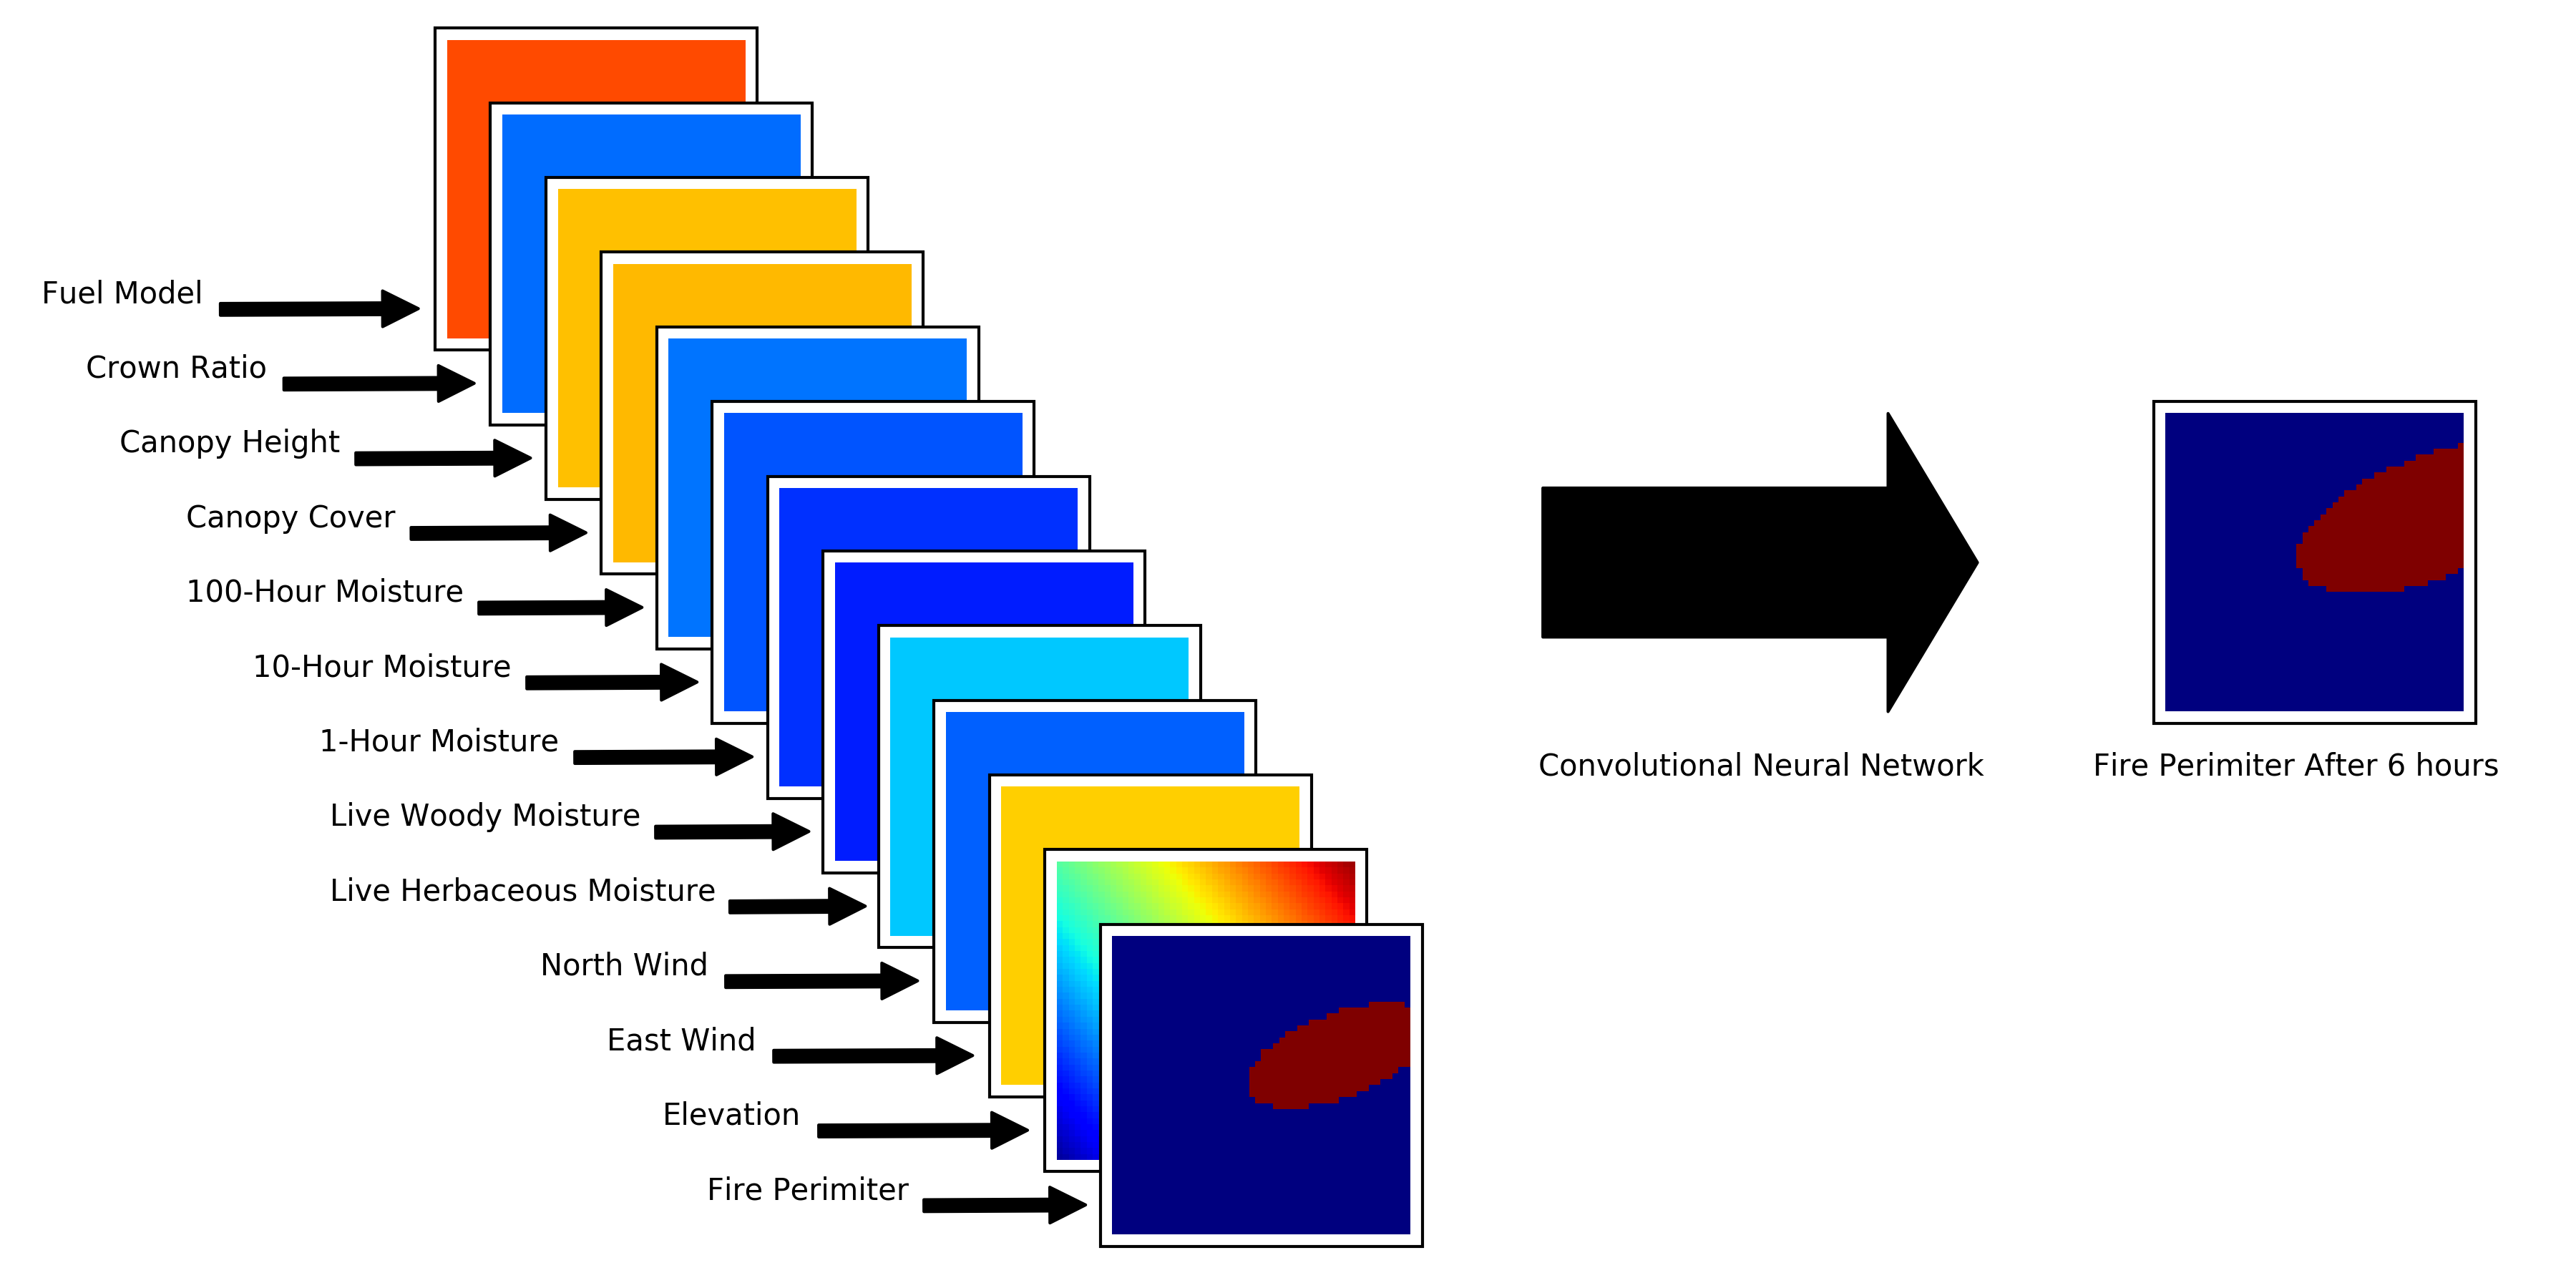
\includegraphics[width=0.95\textwidth]{inputsExampleSingleFire.png}
% figure caption is below the figure
\caption{Schematic of solution algorithm. The left set of images show the
different channels used as inputs to the neural network. The values for each
data channel are colorized based on the values shown in
Table~\ref{tab:paramsLimits} and Table~\ref{tab:paramsExample}.}
\label{fig:exampleIO}       % Give a unique label
\end{figure*}



\subsection{Wildland Fire Prediction}
\label{ss:Wfp}

Data for this study was generated using the surface fire spread model
presented by Rothermel/Albini
\cite{rothermel1972mathematical,scott2005standard,albini1976estimating}.
In the Rothermel/Alibini phenomological model, the peak surface fire
spread rate, $V_{s,peak}$ is calculated using the equation
\begin{equation}
V_{s,peak} = \frac{Q''\zeta}{\rho\epsilon Q_{ig}}\left(1+\phi_{s}+\phi_{w}\right)
\label{eq:rothermel}
\end{equation}
where $Q''$ is the heat release rate per unit area, $\rho$ is the
fuel density, $Q_{ig}$ is the heat of pre-ignition, $\zeta$ is the
propagating flux ratio (percentage of heat released which pre-ignites
fuel), $\epsilon$ is the effective heating number (percentage of fuel
which is involved in ignition), $\phi_{s}$ is the wind coefficient,
and $\phi_{s}$ is the slope coefficient.

Various researchers have developed empirical relationships for the
different parameters in Eq.~\ref{eq:rothermel}. A commonly used approach
in the literature is to specify $Q''$, $\rho$, $\zeta$, $\epsilon$
based on classifying the primary fuel in a region into a fuel model.
A total of 53 fuel models were considered in this work including
13 developed by Rothermal/Albini \cite{rothermel1972mathematical,albini1976estimating},
and 40 developed by Scott \cite{scott2005standard}. Rothermel presented
an empirical relationship for $Q_{ig}$ based on the fuel model and
moisture content, and Scott extended the relationship to handle dynamic
fuel models. Rothermel presented empirical relationships for $\phi_{w}$
and $\phi_{s}$ based on fuel model, midflame wind speed, and slope.
Andrews presented an algorithm to adjust typical atmospheric wind
measurements (10m or 20ft) to mindflame wind speed based on three
additional parameters describing the upper story vegetation
(canopy cover, canopy height, and crown ratio)
\cite{andrews2012modeling}. Researchers have shown wildland fires grow
in a generally ellipsoidal shape for homogenous spatial conditions
based on $V_{s,peak}$ and wind speed
\cite{finney1999mechanistic,wagner1969simple,green1983fire}.
For additional details on the empirical relationships and fuel models the
reader is referred to the original publications.

The primary drivers in this model were identified as
landscape (slope, aspect, and fuel model type),
moisture content (1-hour, 10-hour, 100-hour, live woody, and live herbaceous),
canopy type (height, ratio, and percent coverage),
and 10m wind (intensity and direction). The allowable bounds used for
each parameter in this work are shown in Table~\ref{tab:paramsLimits}.
The fuel model types were assigned indexes based on the peak rate of spread
under the same spread conditions (low moisture, 10 mph wind up a 0.5 slope).
Since slope and aspect can be summarized as a 2-D difference in elevation,
a single channel for elevation was used instead of two channels for slope
and aspect in the neural network.

% For tables use
\begin{table}[htb]
\centering
% table caption is above the table
\caption{Limits of each parameter in study.}
\label{tab:paramsLimits}       % Give a unique label
% For LaTeX tables use
\begin{tabular}{llll}
\hline\noalign{\smallskip}
Parameter & Unit & Min & Max  \\
\noalign{\smallskip}\hline\noalign{\smallskip}
Aspect & Degrees & 0.0 & 360 \\
Fuel Model & Index & 0.0 & 53 \\
Slope & Fraction & 0.0 & 1.0 \\
\hline
1-Hr Moisture & Percent & 1.0 & 40 \\
10-Hr Moisture & Percent & 1.0 & 40 \\
100-Hr Moisture & Percent & 1.0 & 40 \\
Live Herbaceous Moisture & Percent & 30 & 100 \\
Live Woody Moisture & Percent & 30 & 100 \\
\hline
Canopy Cover & Percent & 0.0 & 1.0 \\
Canopy Height & Feet & 1.0 & 20 \\
Crown Ratio & Fraction & 0.1 & 1.0 \\
\hline
Wind Direction & Degrees & 0.0 & 360 \\
Wind Velocity & Mi/Hr & 0.0 & 30 \\
\noalign{\smallskip}\hline
\end{tabular}
\end{table}

Custom software was developed
to simulate the fire perimeter at 6 hours intervals for 10,000
different combinations of these parameters. 
Raster images of the fire perimeters were generated at a resolution of
1 pixel/km every 6 hours. Example fire perimeters from one simulation
are shown in Fig.~\ref{fig:firePerimeters} for the parameter values
shown in Table~\ref{tab:paramsExample}. The implemention of
Rothermel's model in BehavePlus was used to validate the simulation
framework \cite{andrews2009behaveplus}.



\begin{figure}
\centering
% Use the relevant command to insert your figure file.
% For example, with the graphicx package use
  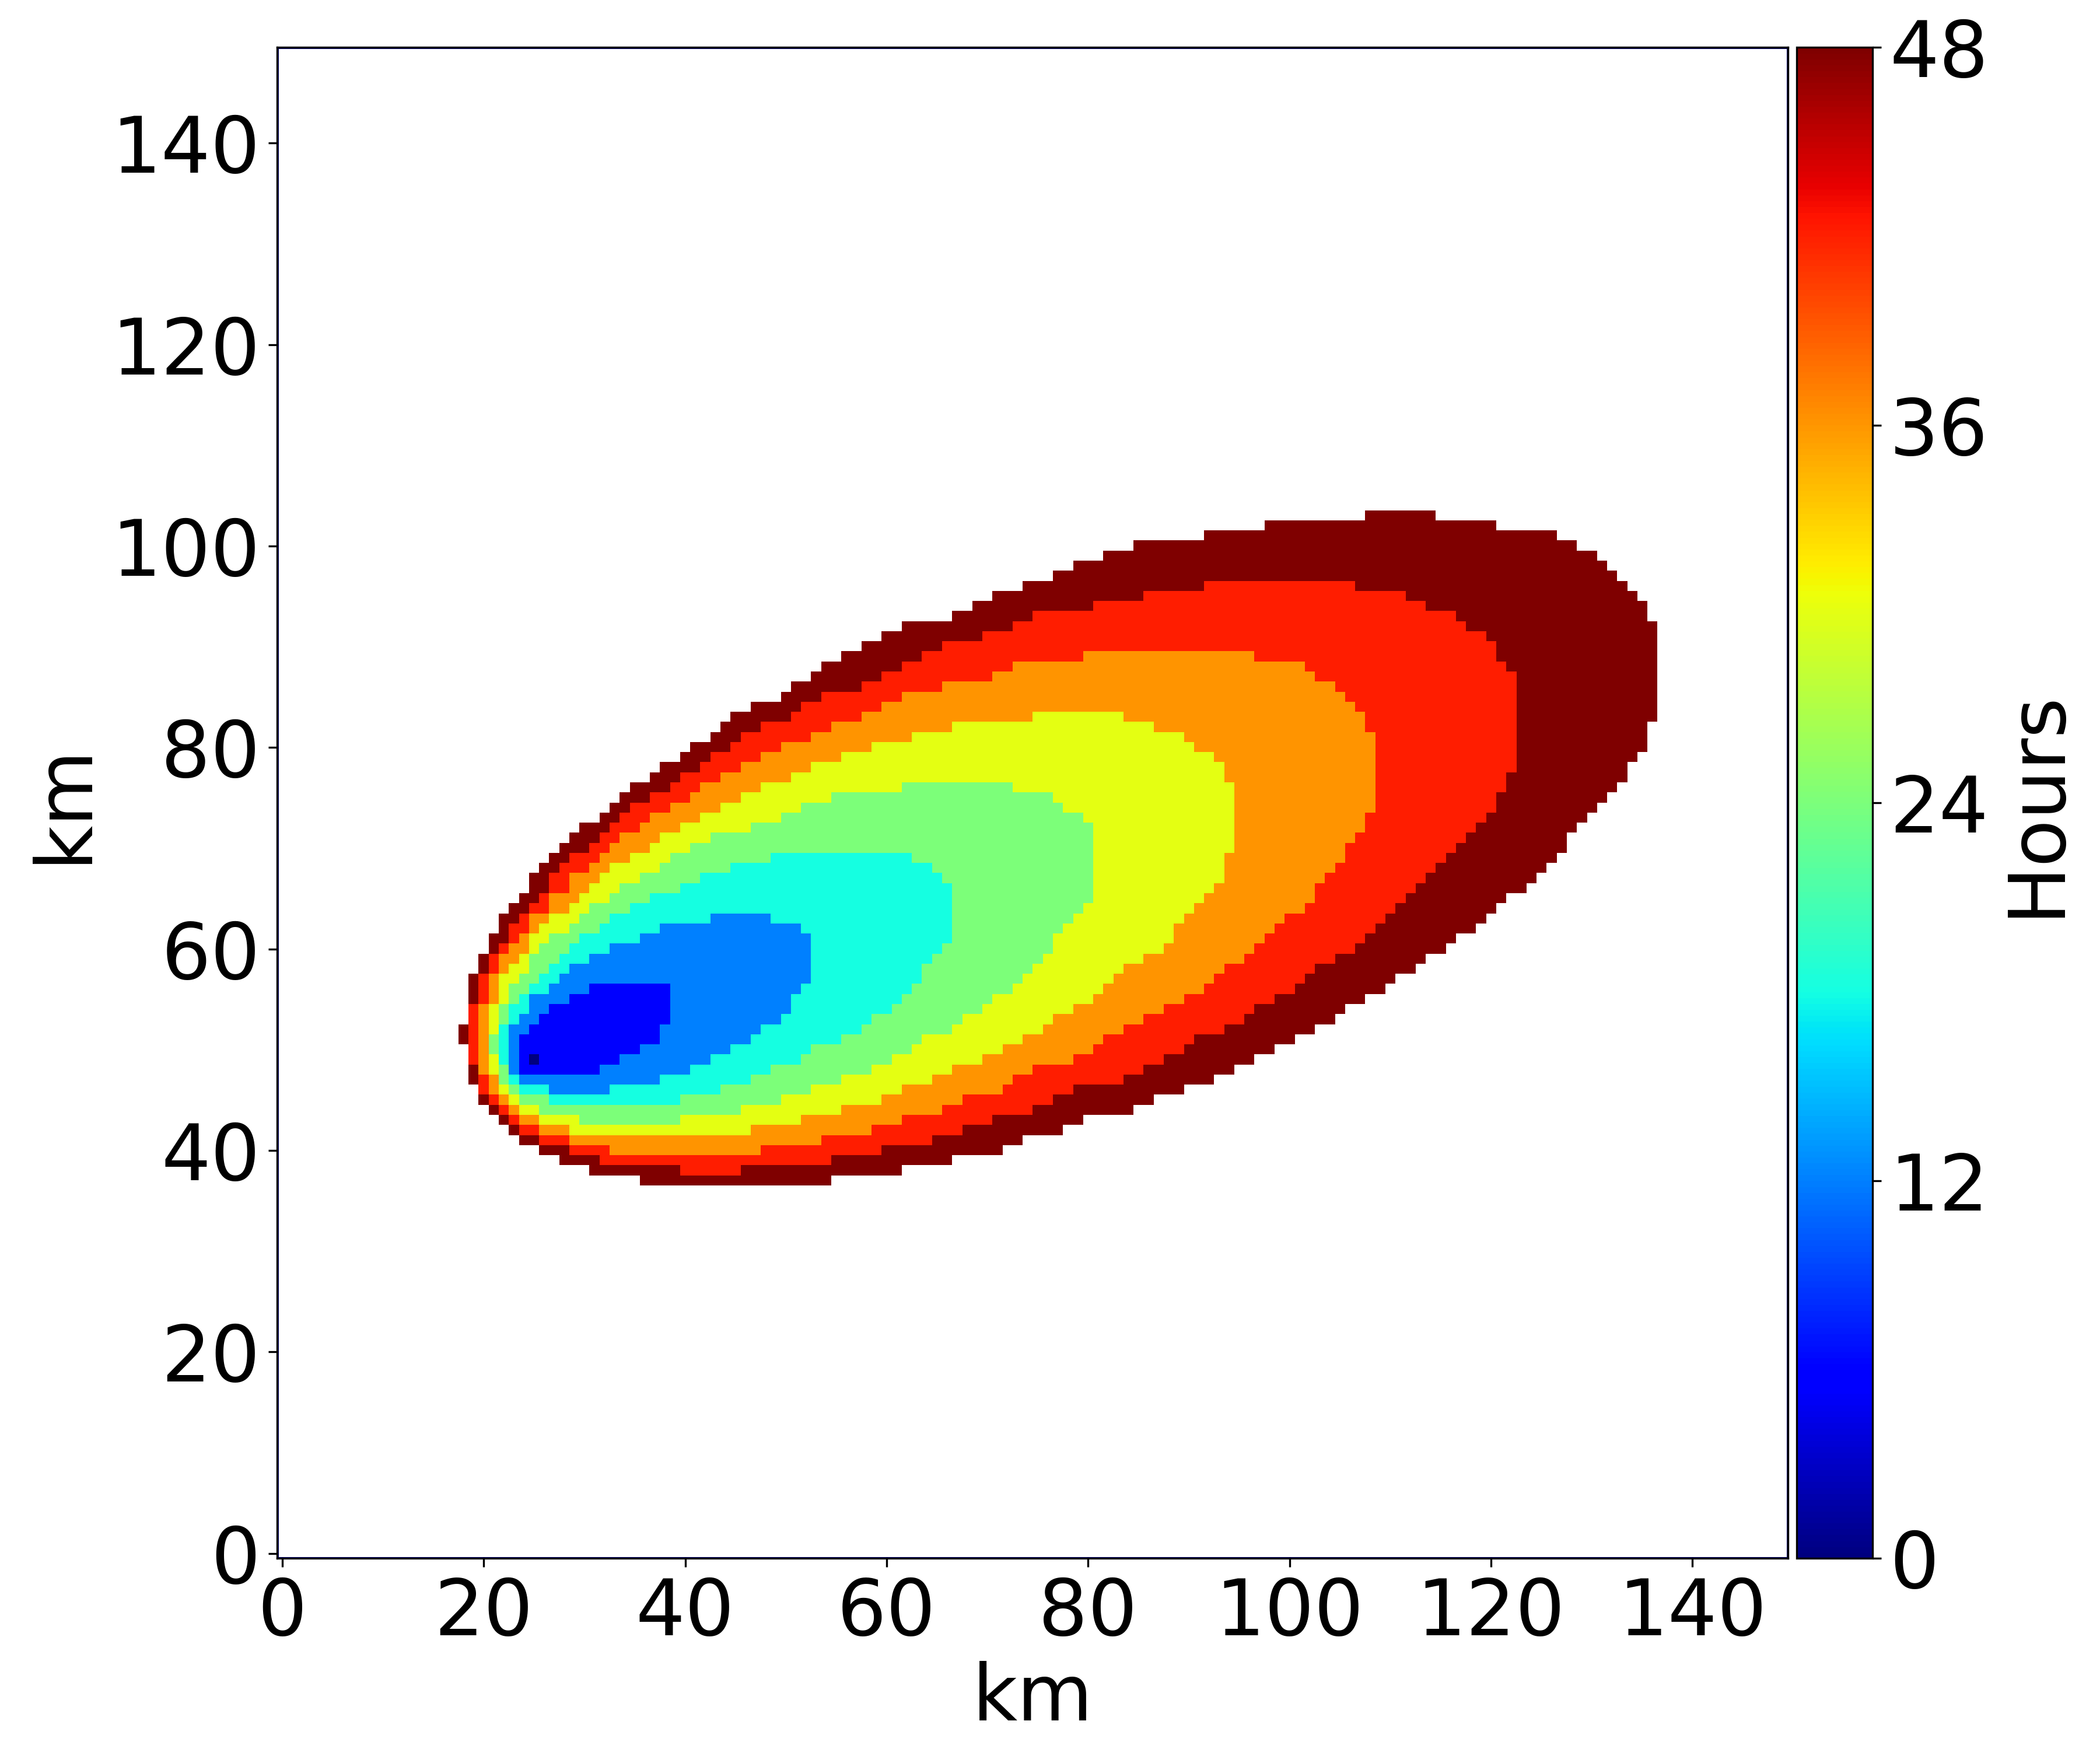
\includegraphics[width=0.45\textwidth]{exampleFirePerimiter0.png}
% figure caption is below the figure
\caption{Example Simulated Fire Perimeter}
\label{fig:firePerimeters}       % Give a unique label
\end{figure}

\begin{table}[htb]
\centering
% table caption is above the table
\caption{Parameters for Example Simulation}
\label{tab:paramsExample}       % Give a unique label
% For LaTeX tables use
\begin{tabular}{llll}
\hline\noalign{\smallskip}
Parameter & Unit & Value \\
\noalign{\smallskip}\hline\noalign{\smallskip}
Aspect & Degrees & 130 \\
Fuel Model & Index & FM1 (44) \\
Slope & Fraction & 0.8 \\
\hline
1-Hr Moisture & Percent & 5.3 \\
10-Hr Moisture & Percent & 6.3 \\
100-Hr Moisture & Percent & 7.3 \\
Live Herbaceous Moisture & Percent & 69 \\
Live Woody Moisture & Percent & 49 \\
\hline
Canopy Cover & Percent & 0.7 \\
Canopy Height & Feet & 14 \\
Crown Ratio & Fraction & 0.2 \\
\hline
Wind Direction & Degrees & 34 \\
Wind Velocity & Miles per Hour & 13.5 \\
\noalign{\smallskip}\hline
\end{tabular}
\end{table}
















\subsection{Network Architecture}
\label{ss:Na}


At a fundamental level, artificial neural networks are massively parallel
equations which have the capability to store observed knowledge about a
problem to make predictions of new inputs. A convolutional neural network
(CNN) assumes the input data has distinct
spatial dependence within the input parameters. Since the network
assumes spatial dependence, less connections need to be made to
inputs which are far from each other. This allows a CNN to contain much
fewer connections and parameters than a similarly sized standard feed
forward network with minimal loss in optimal performance for appropriate
problems. This makes it possible to use deeper and more broad hidden
layers without increasing computational requirements beyond what is
feasible on current technology \cite{krizhevsky2012imagenet}.
Representing the spread of a wildland fire front with a CNN is
reasonable as wildland fire spread is a local phenomena \cite{finney1999mechanistic}.

% For two-column wide figures use
\begin{figure*}[htb!]
\centering
% Use the relevant command to insert your figure file.
% For example, with the graphicx package use
  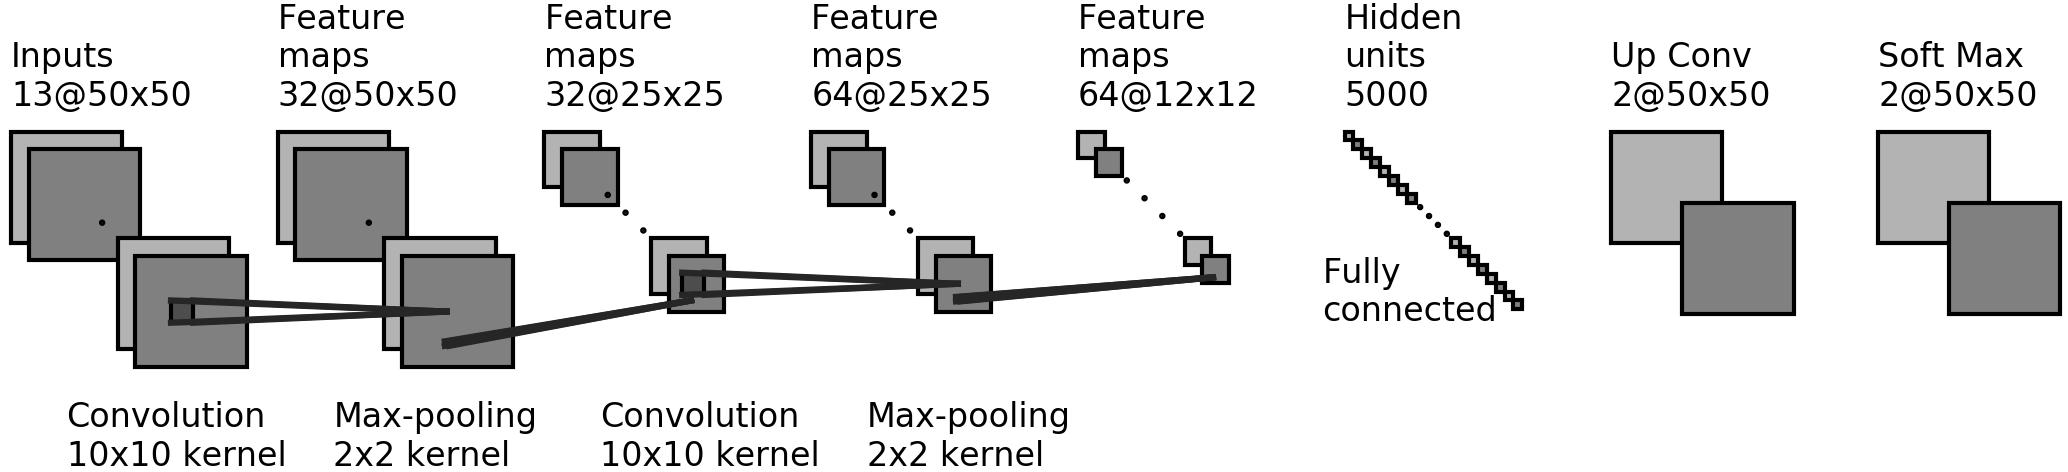
\includegraphics[width=0.95\textwidth]{convnet_fig.png}
% figure caption is below the figure
\caption{Convolutional Neural Network Architecture.}
\label{fig:cnnArchitecture}       % Give a unique label
\end{figure*}

The CNN architecture used in this work is shown in Fig.~\ref{fig:cnnArchitecture}.
The input images were 50x50 pixels with 13 image channels corresponding to the
image stack shown in Fig.~\ref{fig:exampleIO}. The output image contains 50x50 pixels
with two image channels corresponding to the probability the fire perimeter has reached
a pixel and the probability the fire perimeter has not reached a pixel.
A total of 6 hidden layers
are included in the network including 2 convolutional, 2 max pooling, 1 dense
classification, 1 up-convolution, and 1 soft max layers. The number of filters
and step size in each convolutional and up-convolutional and number of neurons
in dense layers were specified to steadily decrease the degrees of freedom from the
32,500 (50x50x13) in the input layer to the desired degrees of freedom of
2,500 (50x50,1) in the output layer. All hidden layers used a leaky rectified
linear unit activation function except the fully connected layer which
used a hyperbolic tangent activation function. The output layer used a soft max
activation function to estimate the probability that each pixel would contain
a fire. Over-fitting was reduced by using 50\% dropout on the input layer.
The cost function used in training was based on sum square error.

The network architecture was built using the Python 3 bindings for TensorFlow
\cite{tensorflow2015-whitepaper}. The network was trained using 27,000 samples
(3 per parameter set) for 50,000 epochs using a single NVIDIA Quadro K620.
The total time to train the network was 18 hours
7 minutes.

%\FloatBarrier

\subsection{Post Processing}
\label{ss:PP}

The output layer of the CNN contains two normalized probability masks, one for
fire and one for not fire. The normalized probability mask for fire is
post-processed to convert the probabilistic estimate of fire perimeter to
a single contour. A 3x3 median filter is applied to smooth the image. A threshold value
on probability of fire is used to determine whether or not each pixel is part of the fire
perimeter. An example neural network prediction before and after post-processing
is shown in Fig.~\ref{fig:postProcess}.
The impact of this threshold on the performance of the model is discussed in
Section~\ref{s:Discussion}.

\begin{figure}[htb]
	\centering
	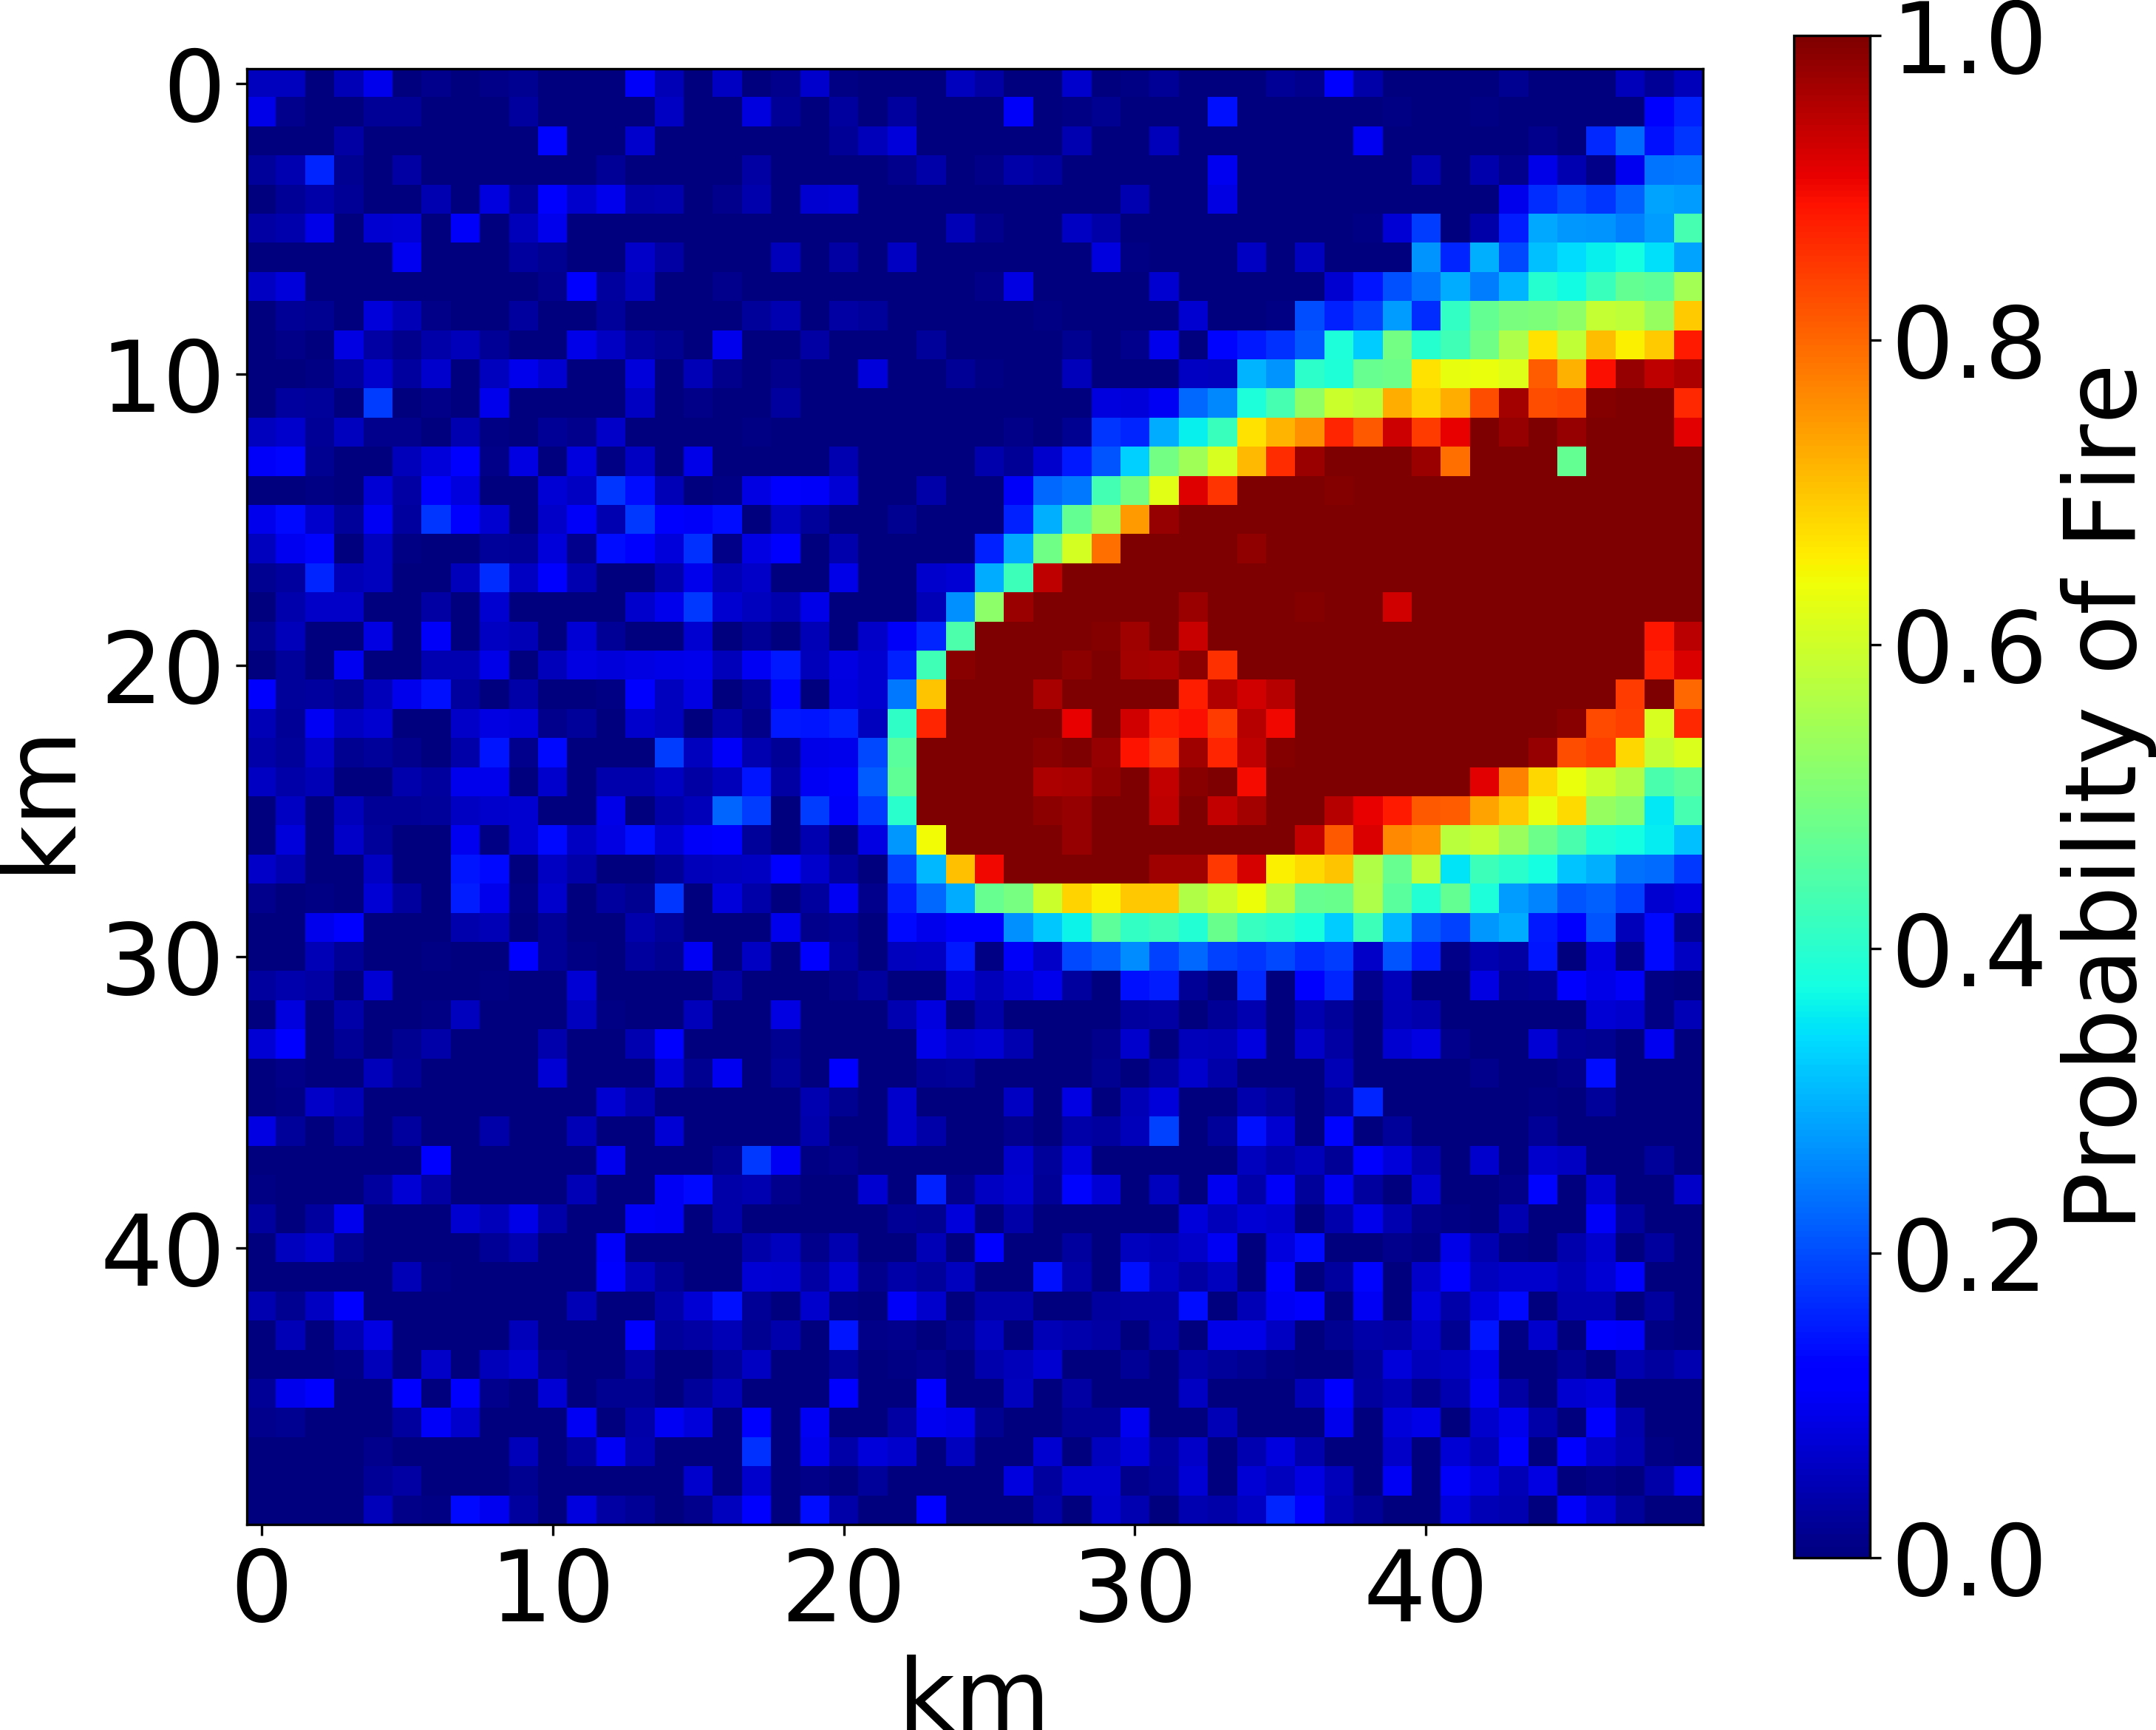
\includegraphics[width=0.23\textwidth]{exampleNetworkRaw0.png}
	~
	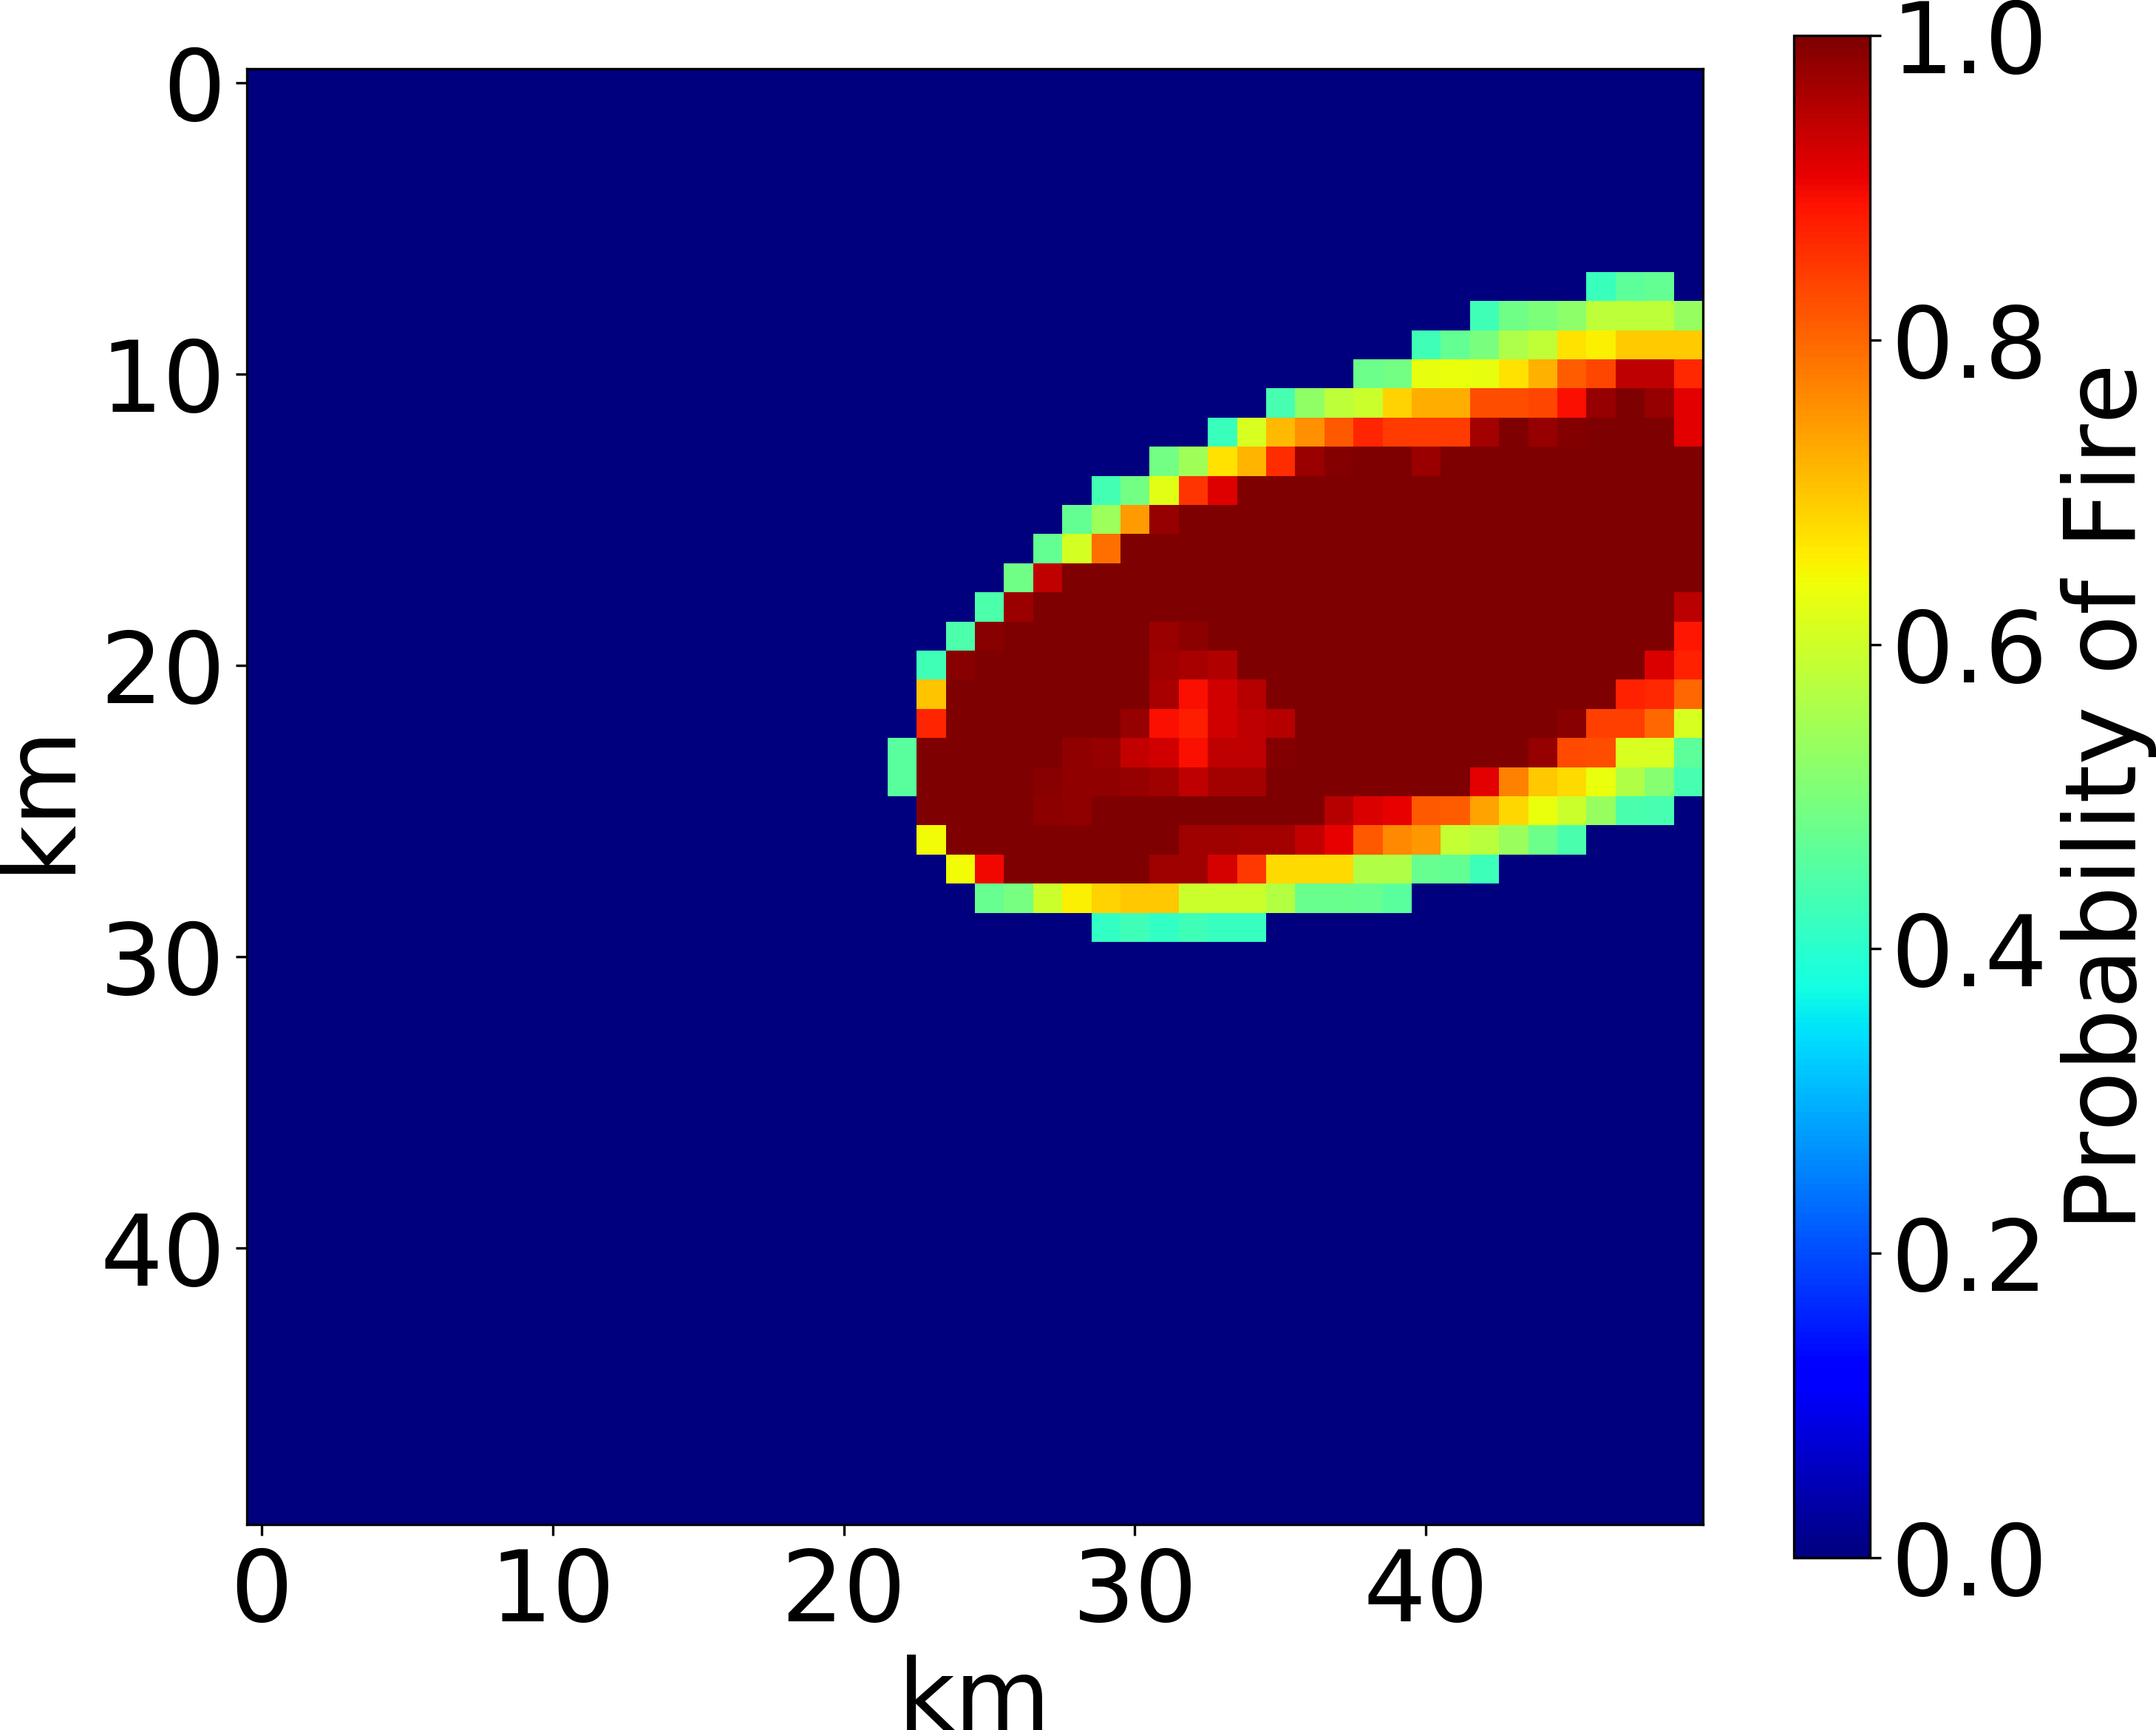
\includegraphics[width=0.23\textwidth]{exampleNetworkProcessed0.png}
	\\
	(a)\hspace{0.23\textwidth}(b)
\caption{Example CNN prediction of fire perimeter probability (a) Directly predicted from CNN (b) After post-processing}
\label{fig:postProcess}       % Give a unique label
\end{figure}



\subsection{Performance Metrics}
\label{ss:PM}

The metrics used to quantify the performance of the CNN in this study
were precision, sensitivity, and F-measure. For each metric, the range
of possible values is 0 to 1, with a perfect score being 1.
The precision, $P$, is defined as
\begin{equation}
P = \frac{t_{p}}{t_{p}+f_{p}}
\label{eq:precision}
\end{equation}
where $t_{p}$ is the number of correctly identified fire pixels, and
$f_{p}$ is the number of falsely identified fire pixels.
The sensitivity, $S$, is defined as
\begin{equation}
S = \frac{t_{p}}{t_{p}+f_{n}}
\label{eq:sensitivity}
\end{equation}
where $f_{n}$ is the number of fire pixels which were identifed
as non-fire pixels.
F-measure is, $F$, is the harmonic mean of $P$ and $S$,
\begin{equation}
F = 2\cdot\frac{P\cdot S}{P+S}.
\label{eq:fmeasure}
\end{equation}






\begin{figure*}[htbp]
  \centering
	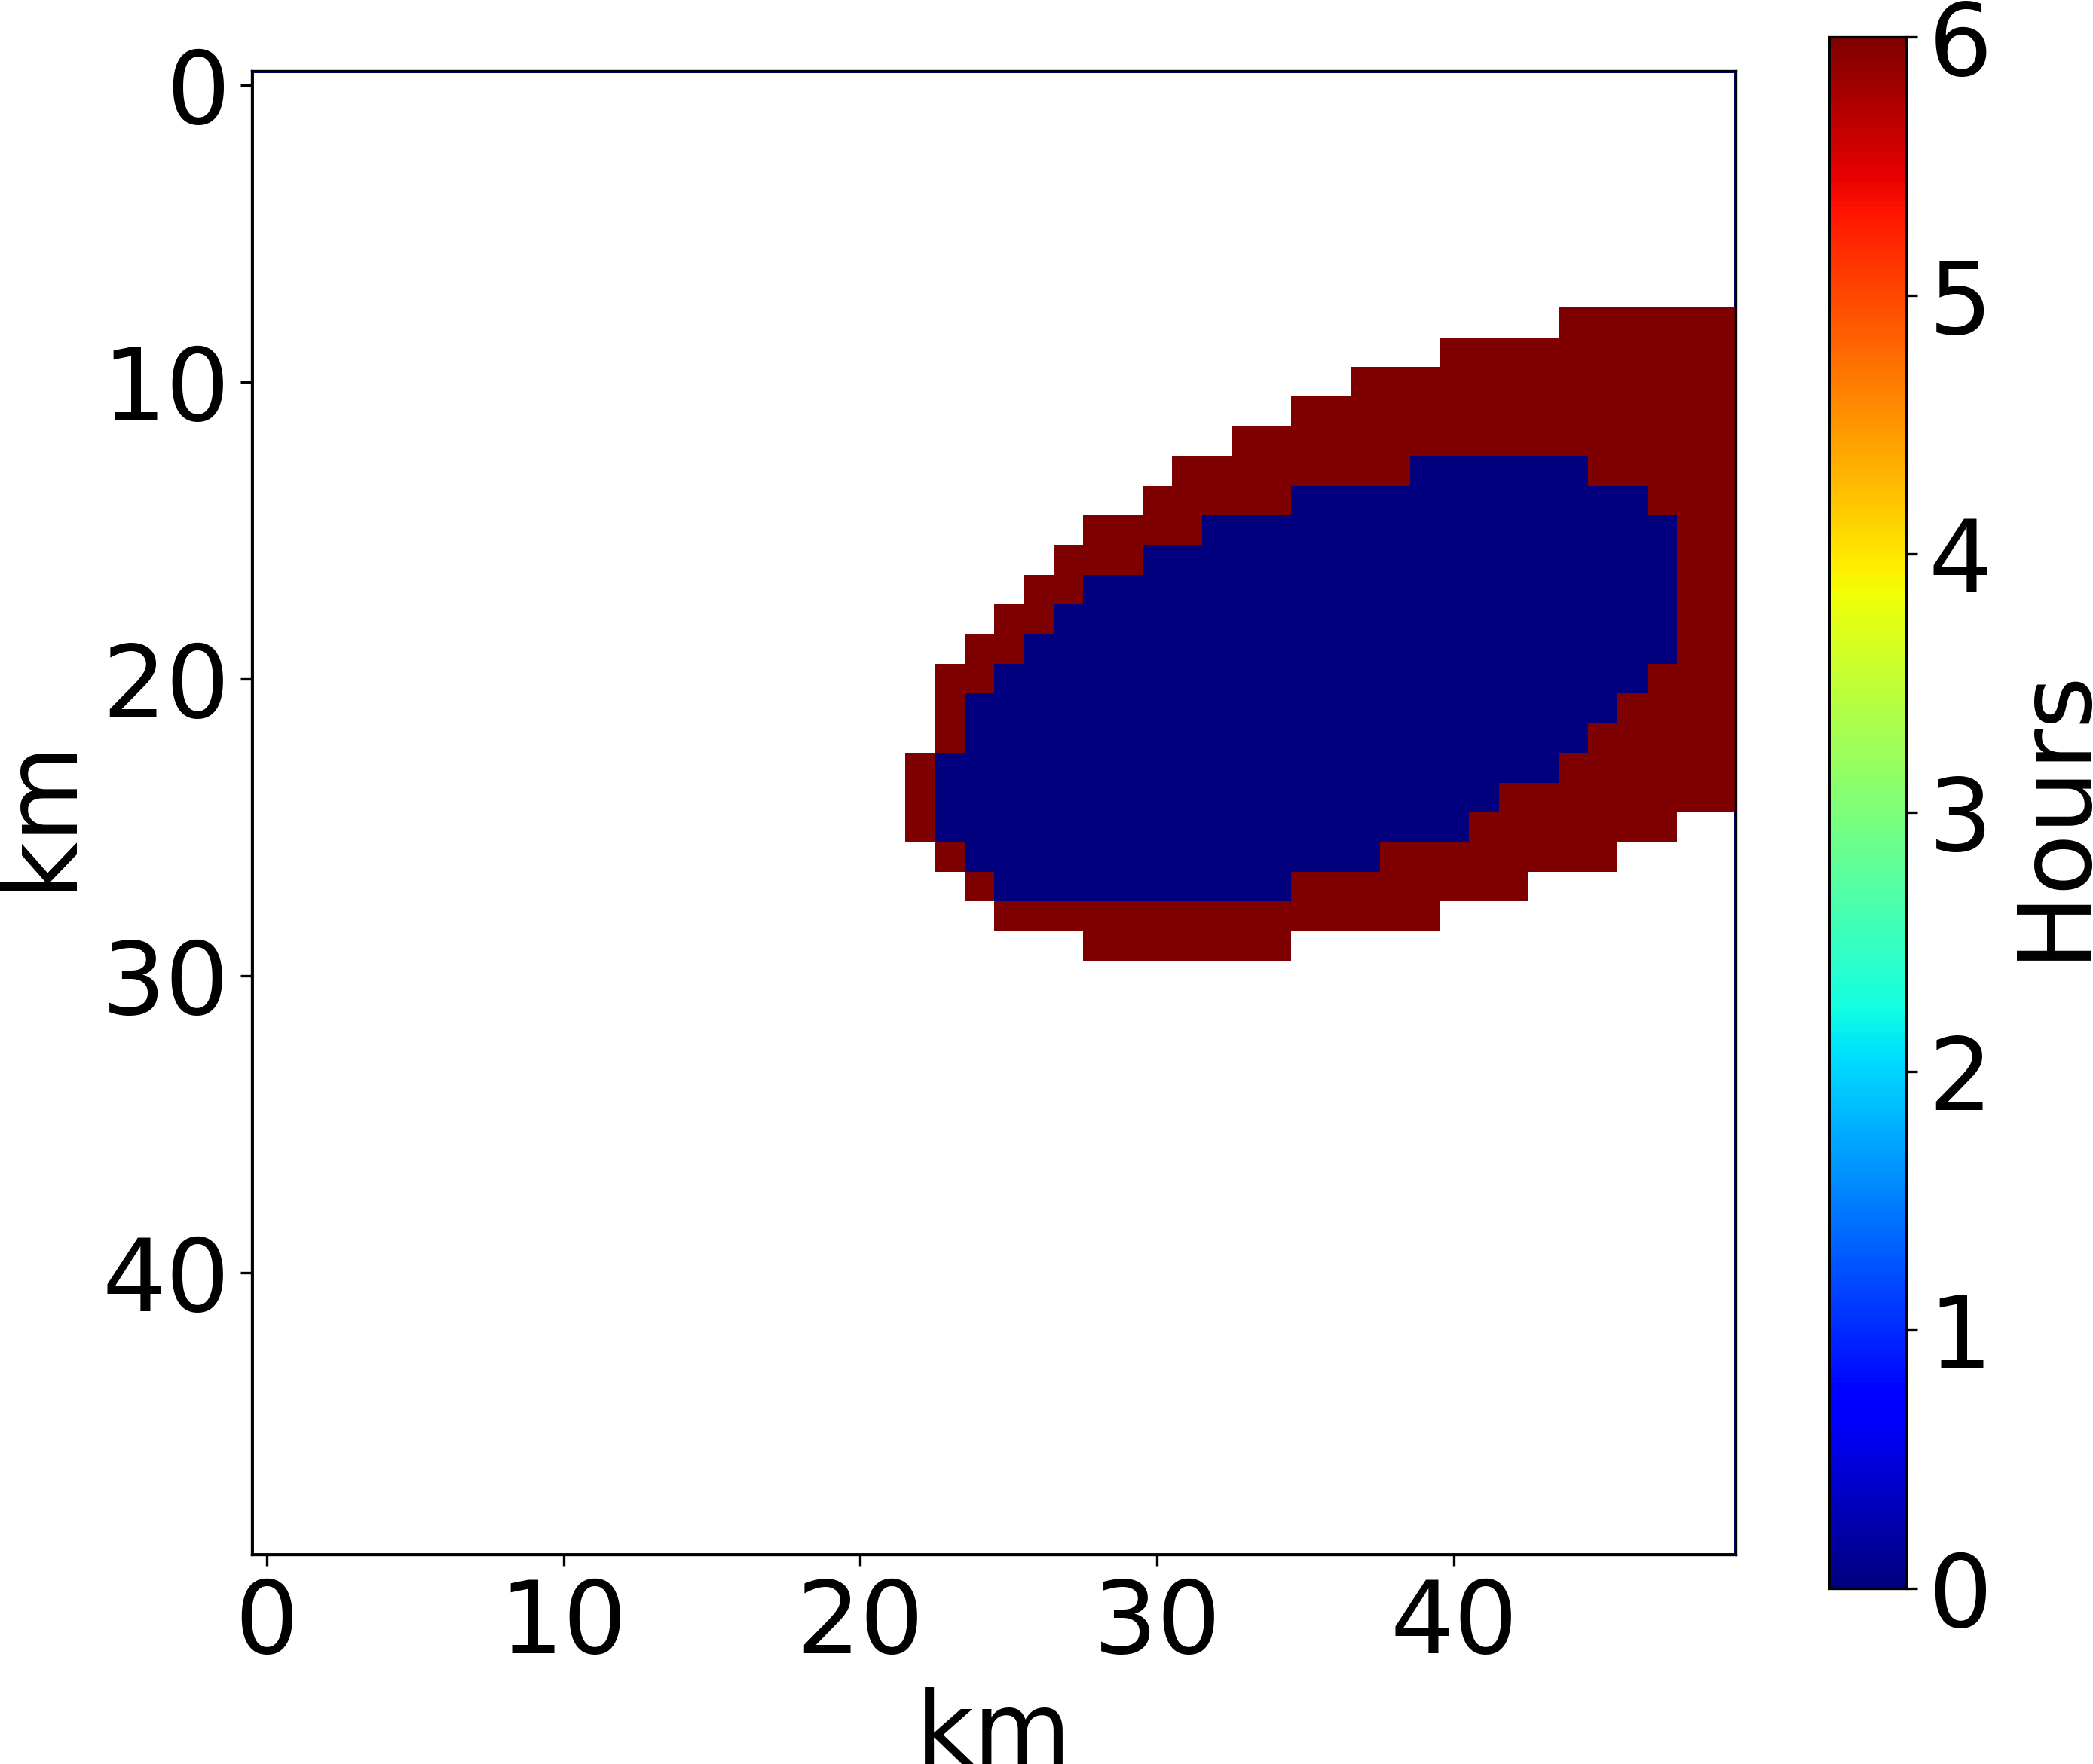
\includegraphics[height=0.25\textwidth]{exampleFusedFire0.png}
	~
	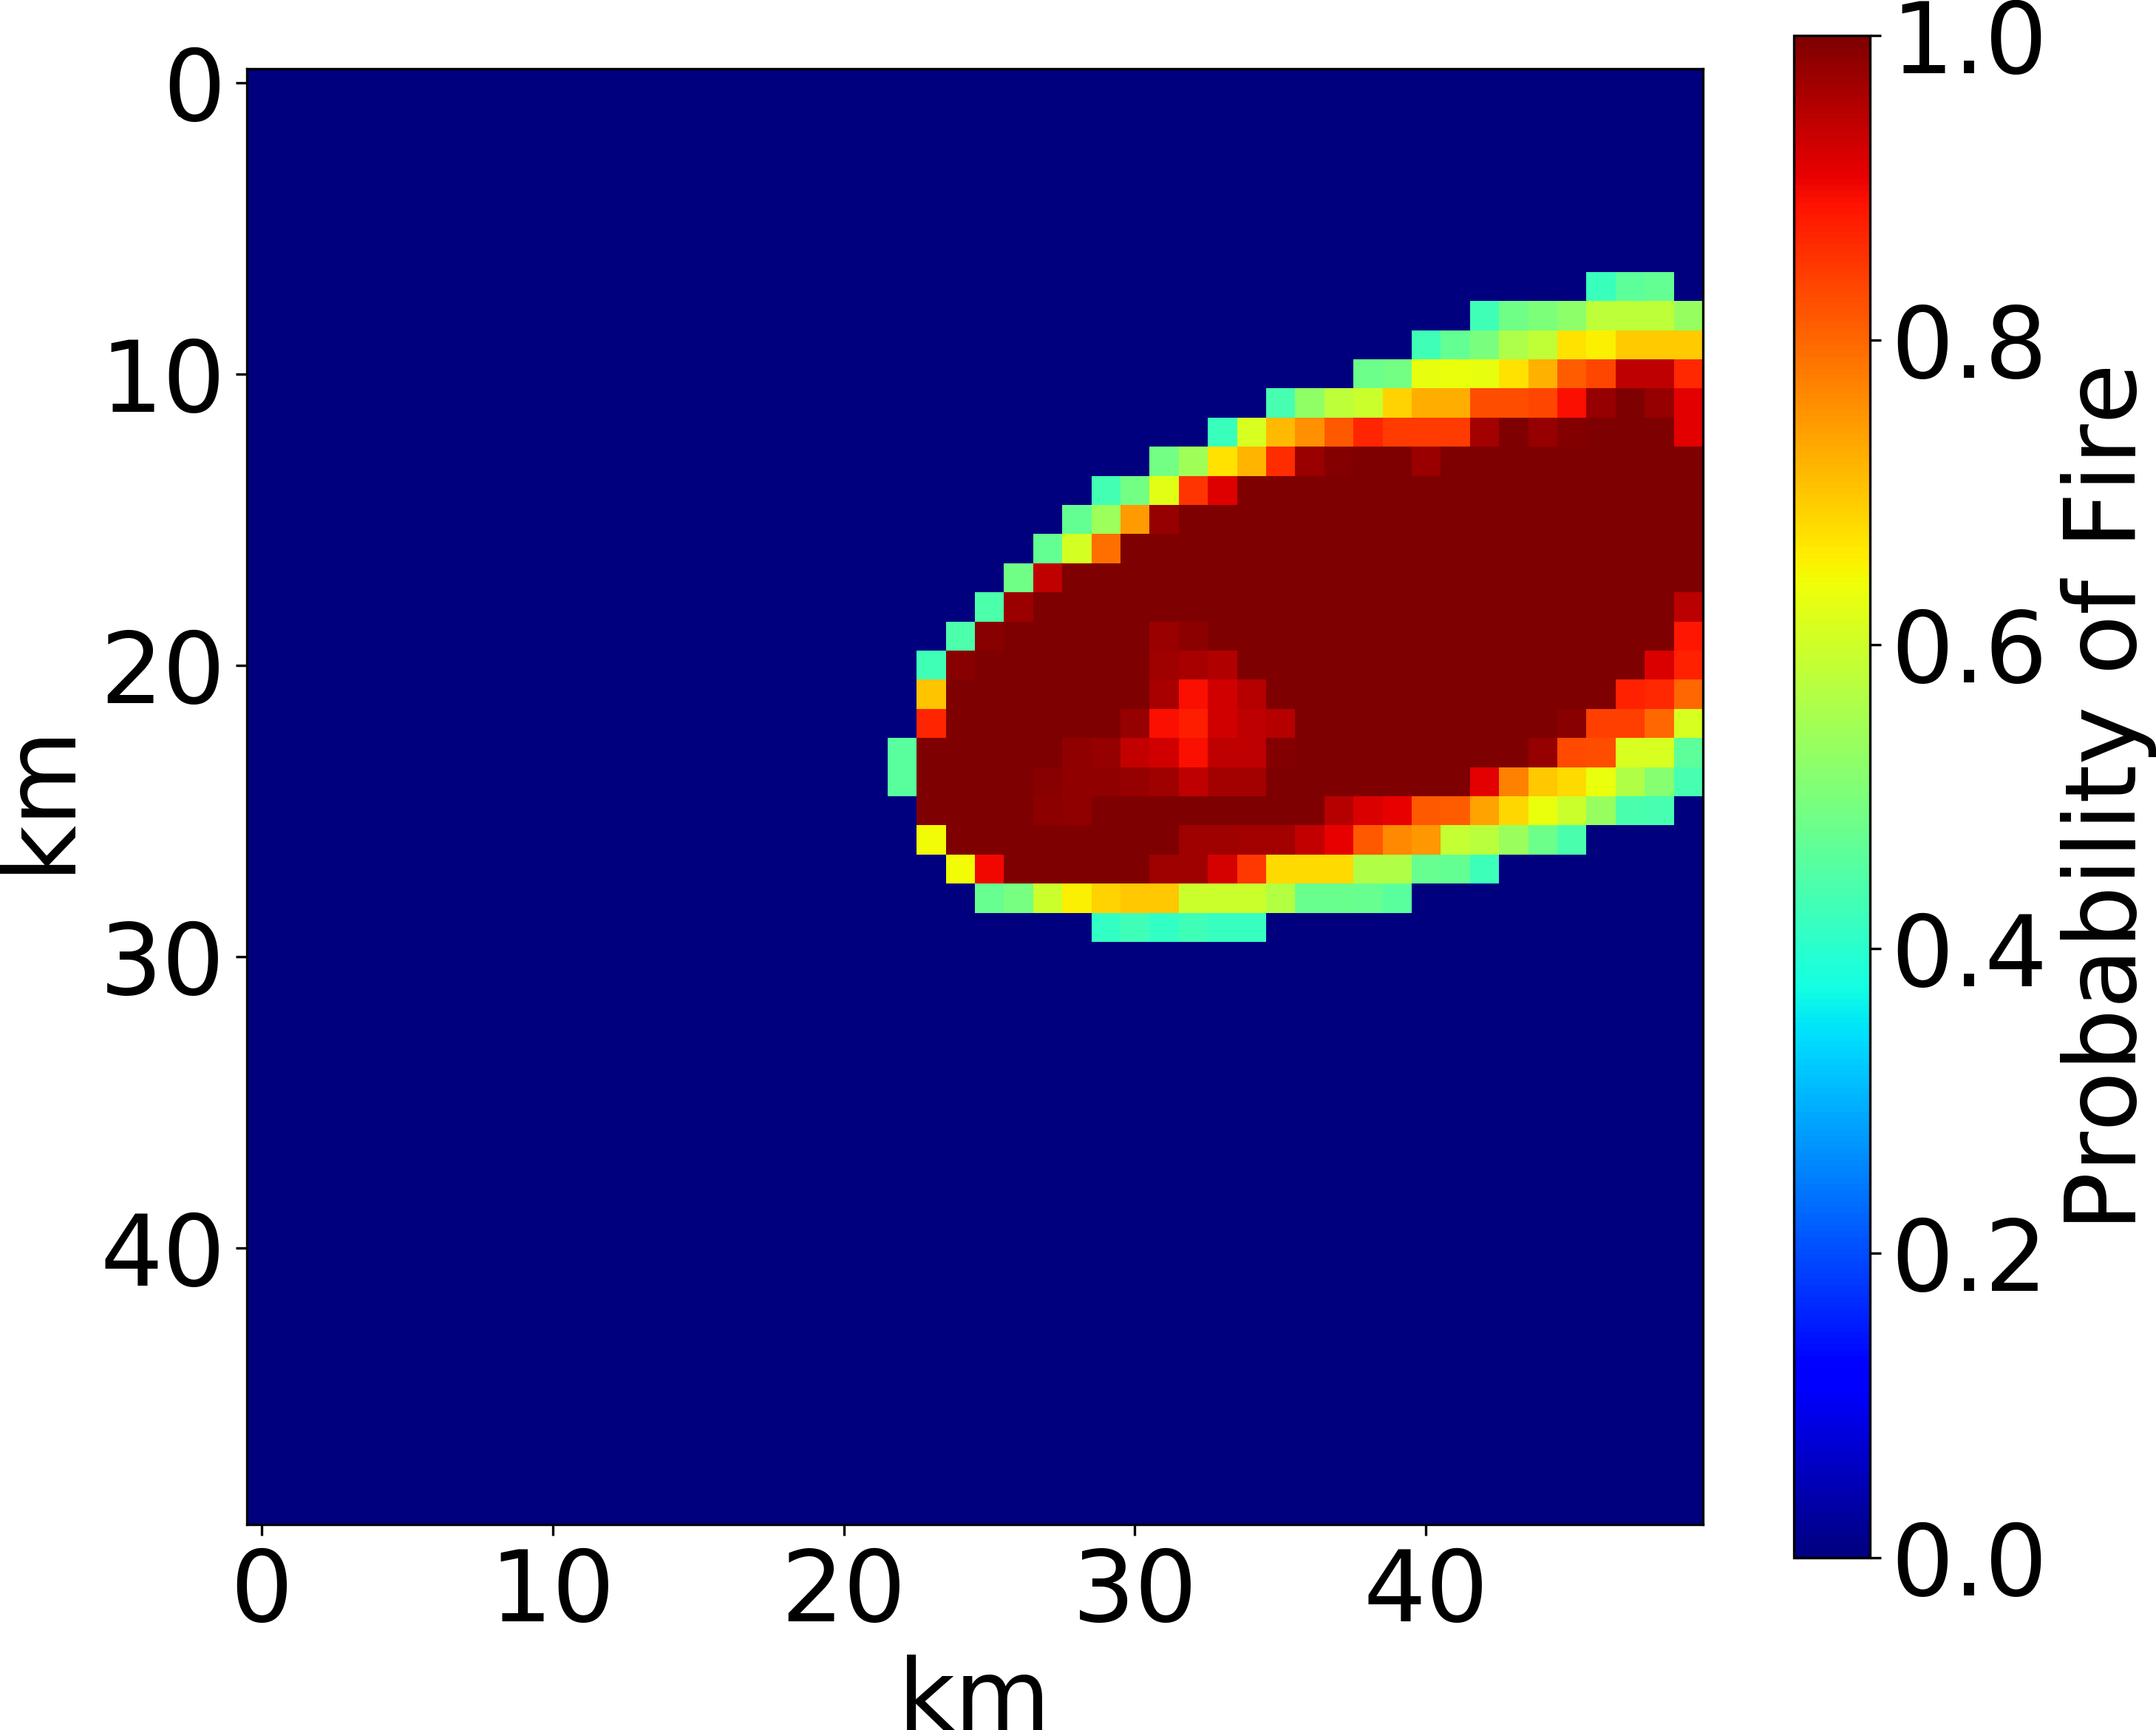
\includegraphics[height=0.25\textwidth]{exampleNetworkProcessed0.png}
	~
	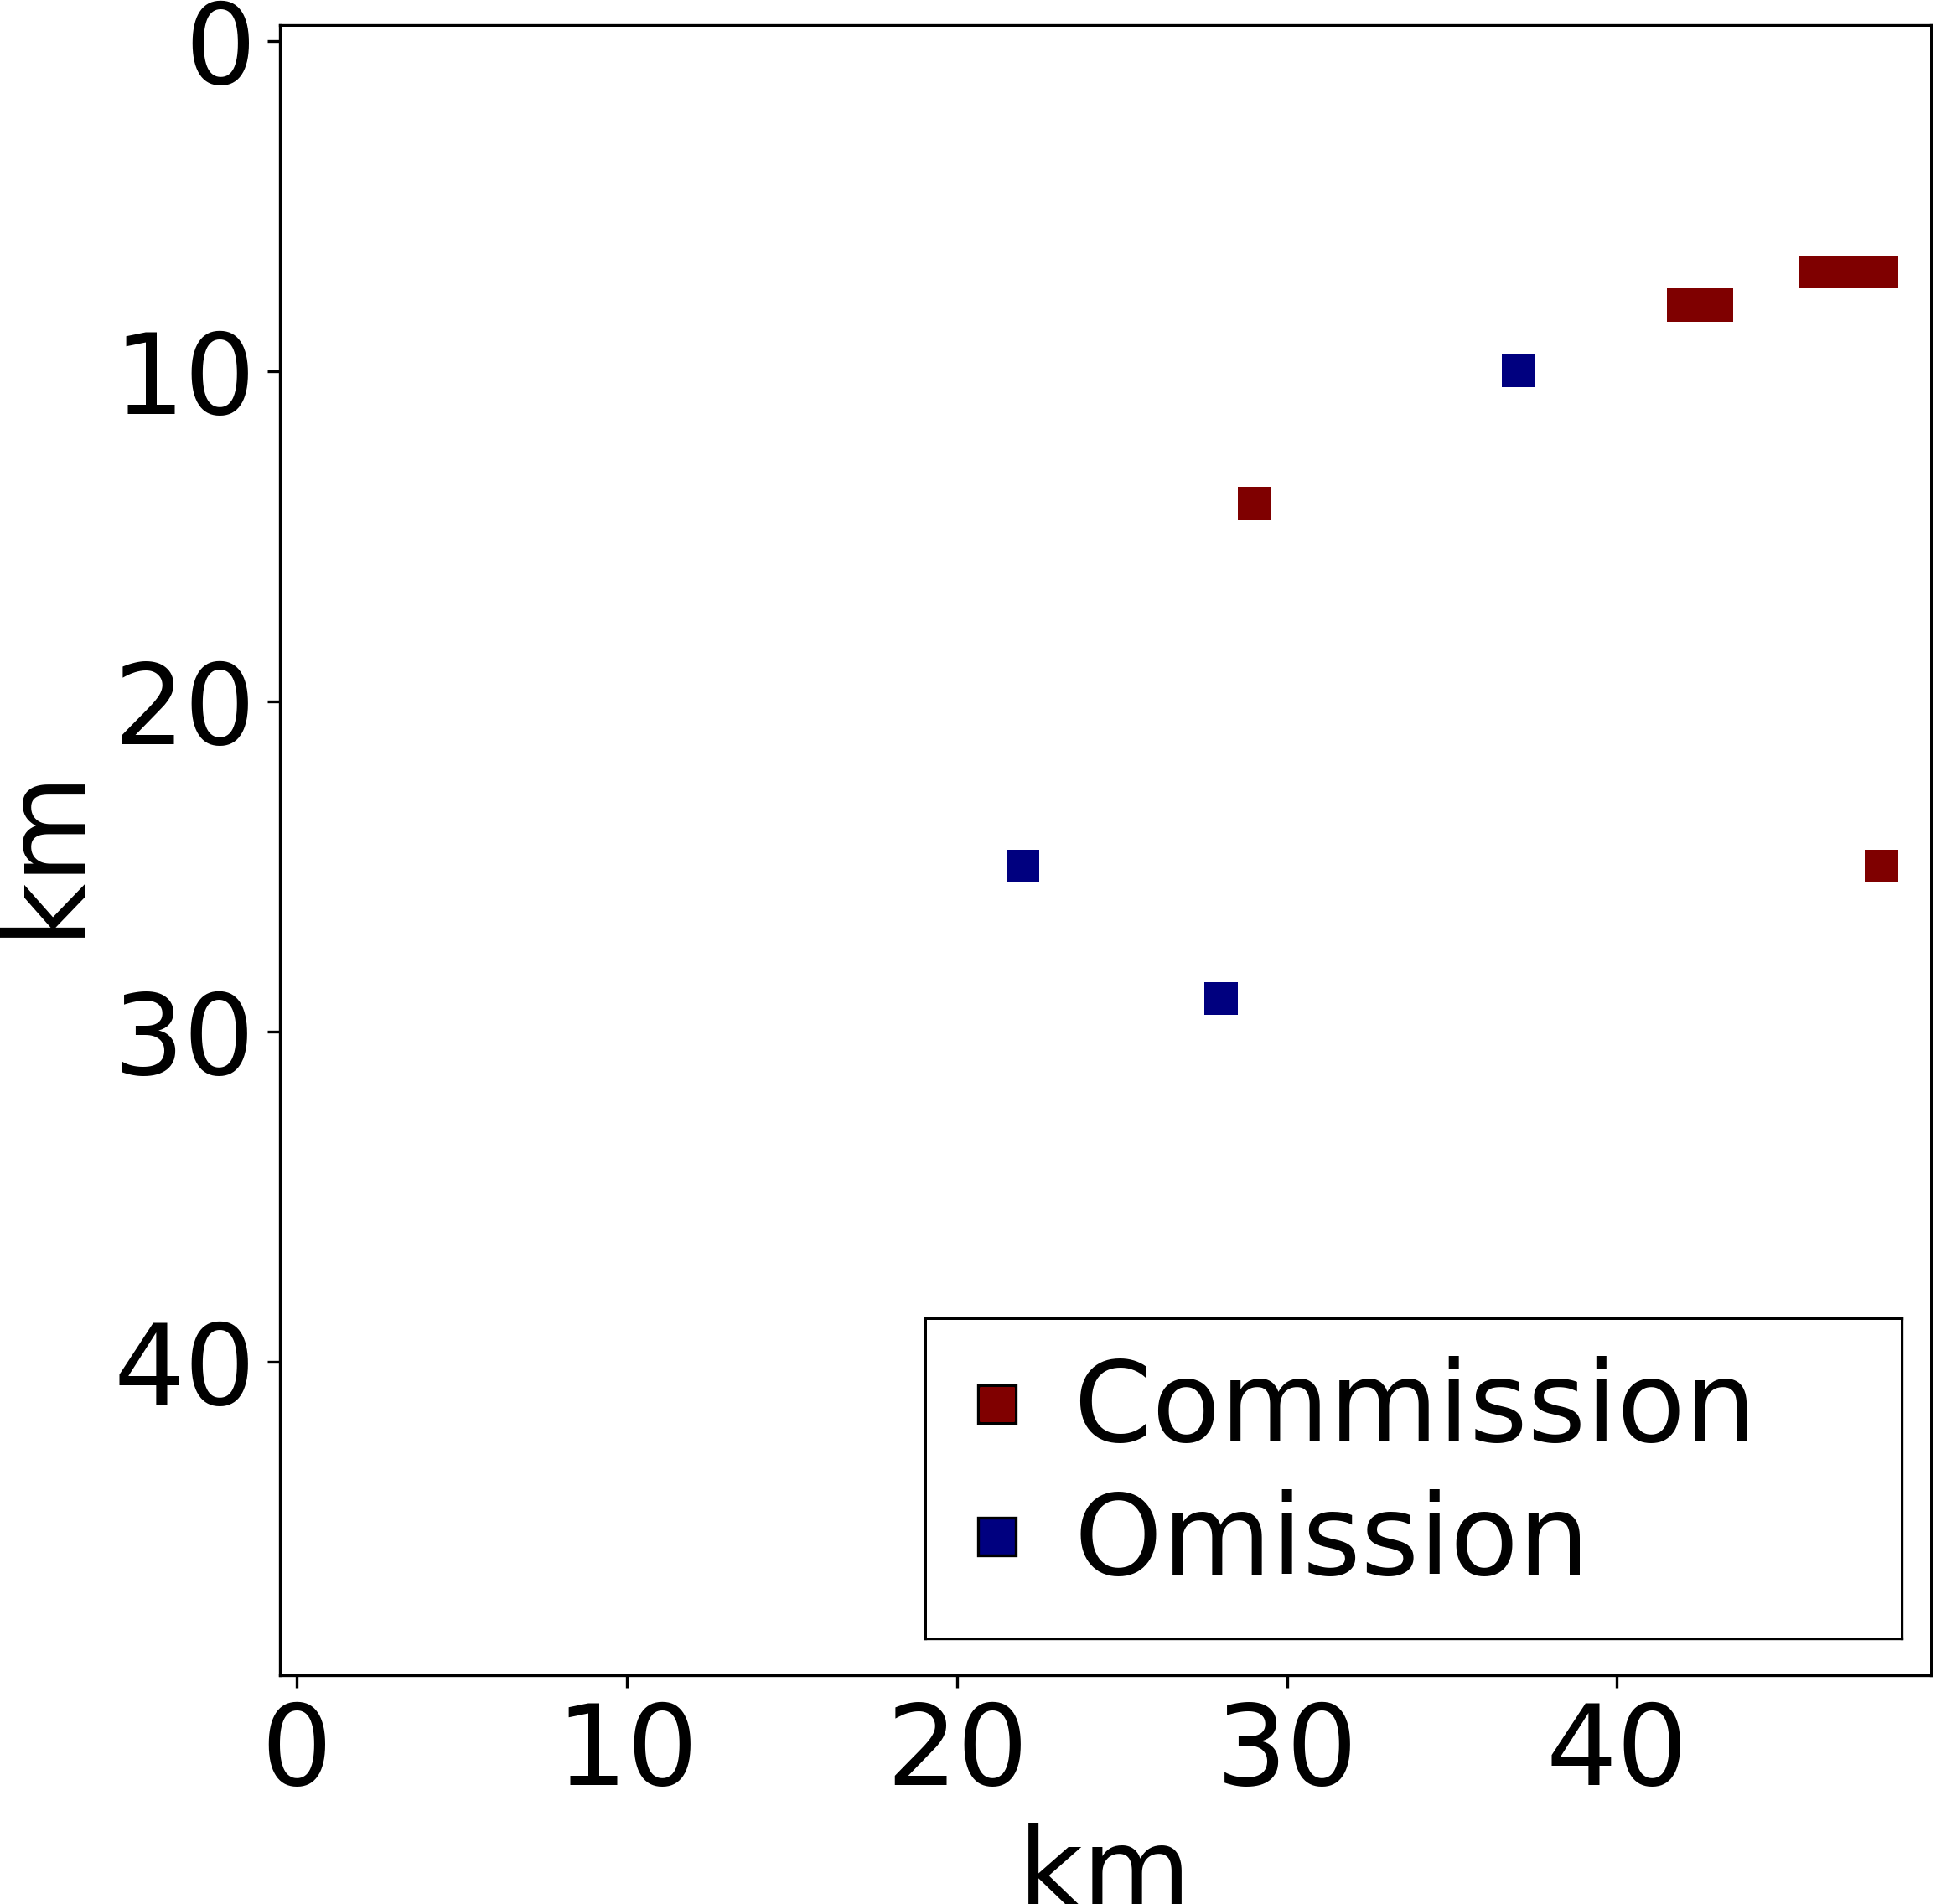
\includegraphics[height=0.25\textwidth]{exampleNetworkError0.png}
	\\
	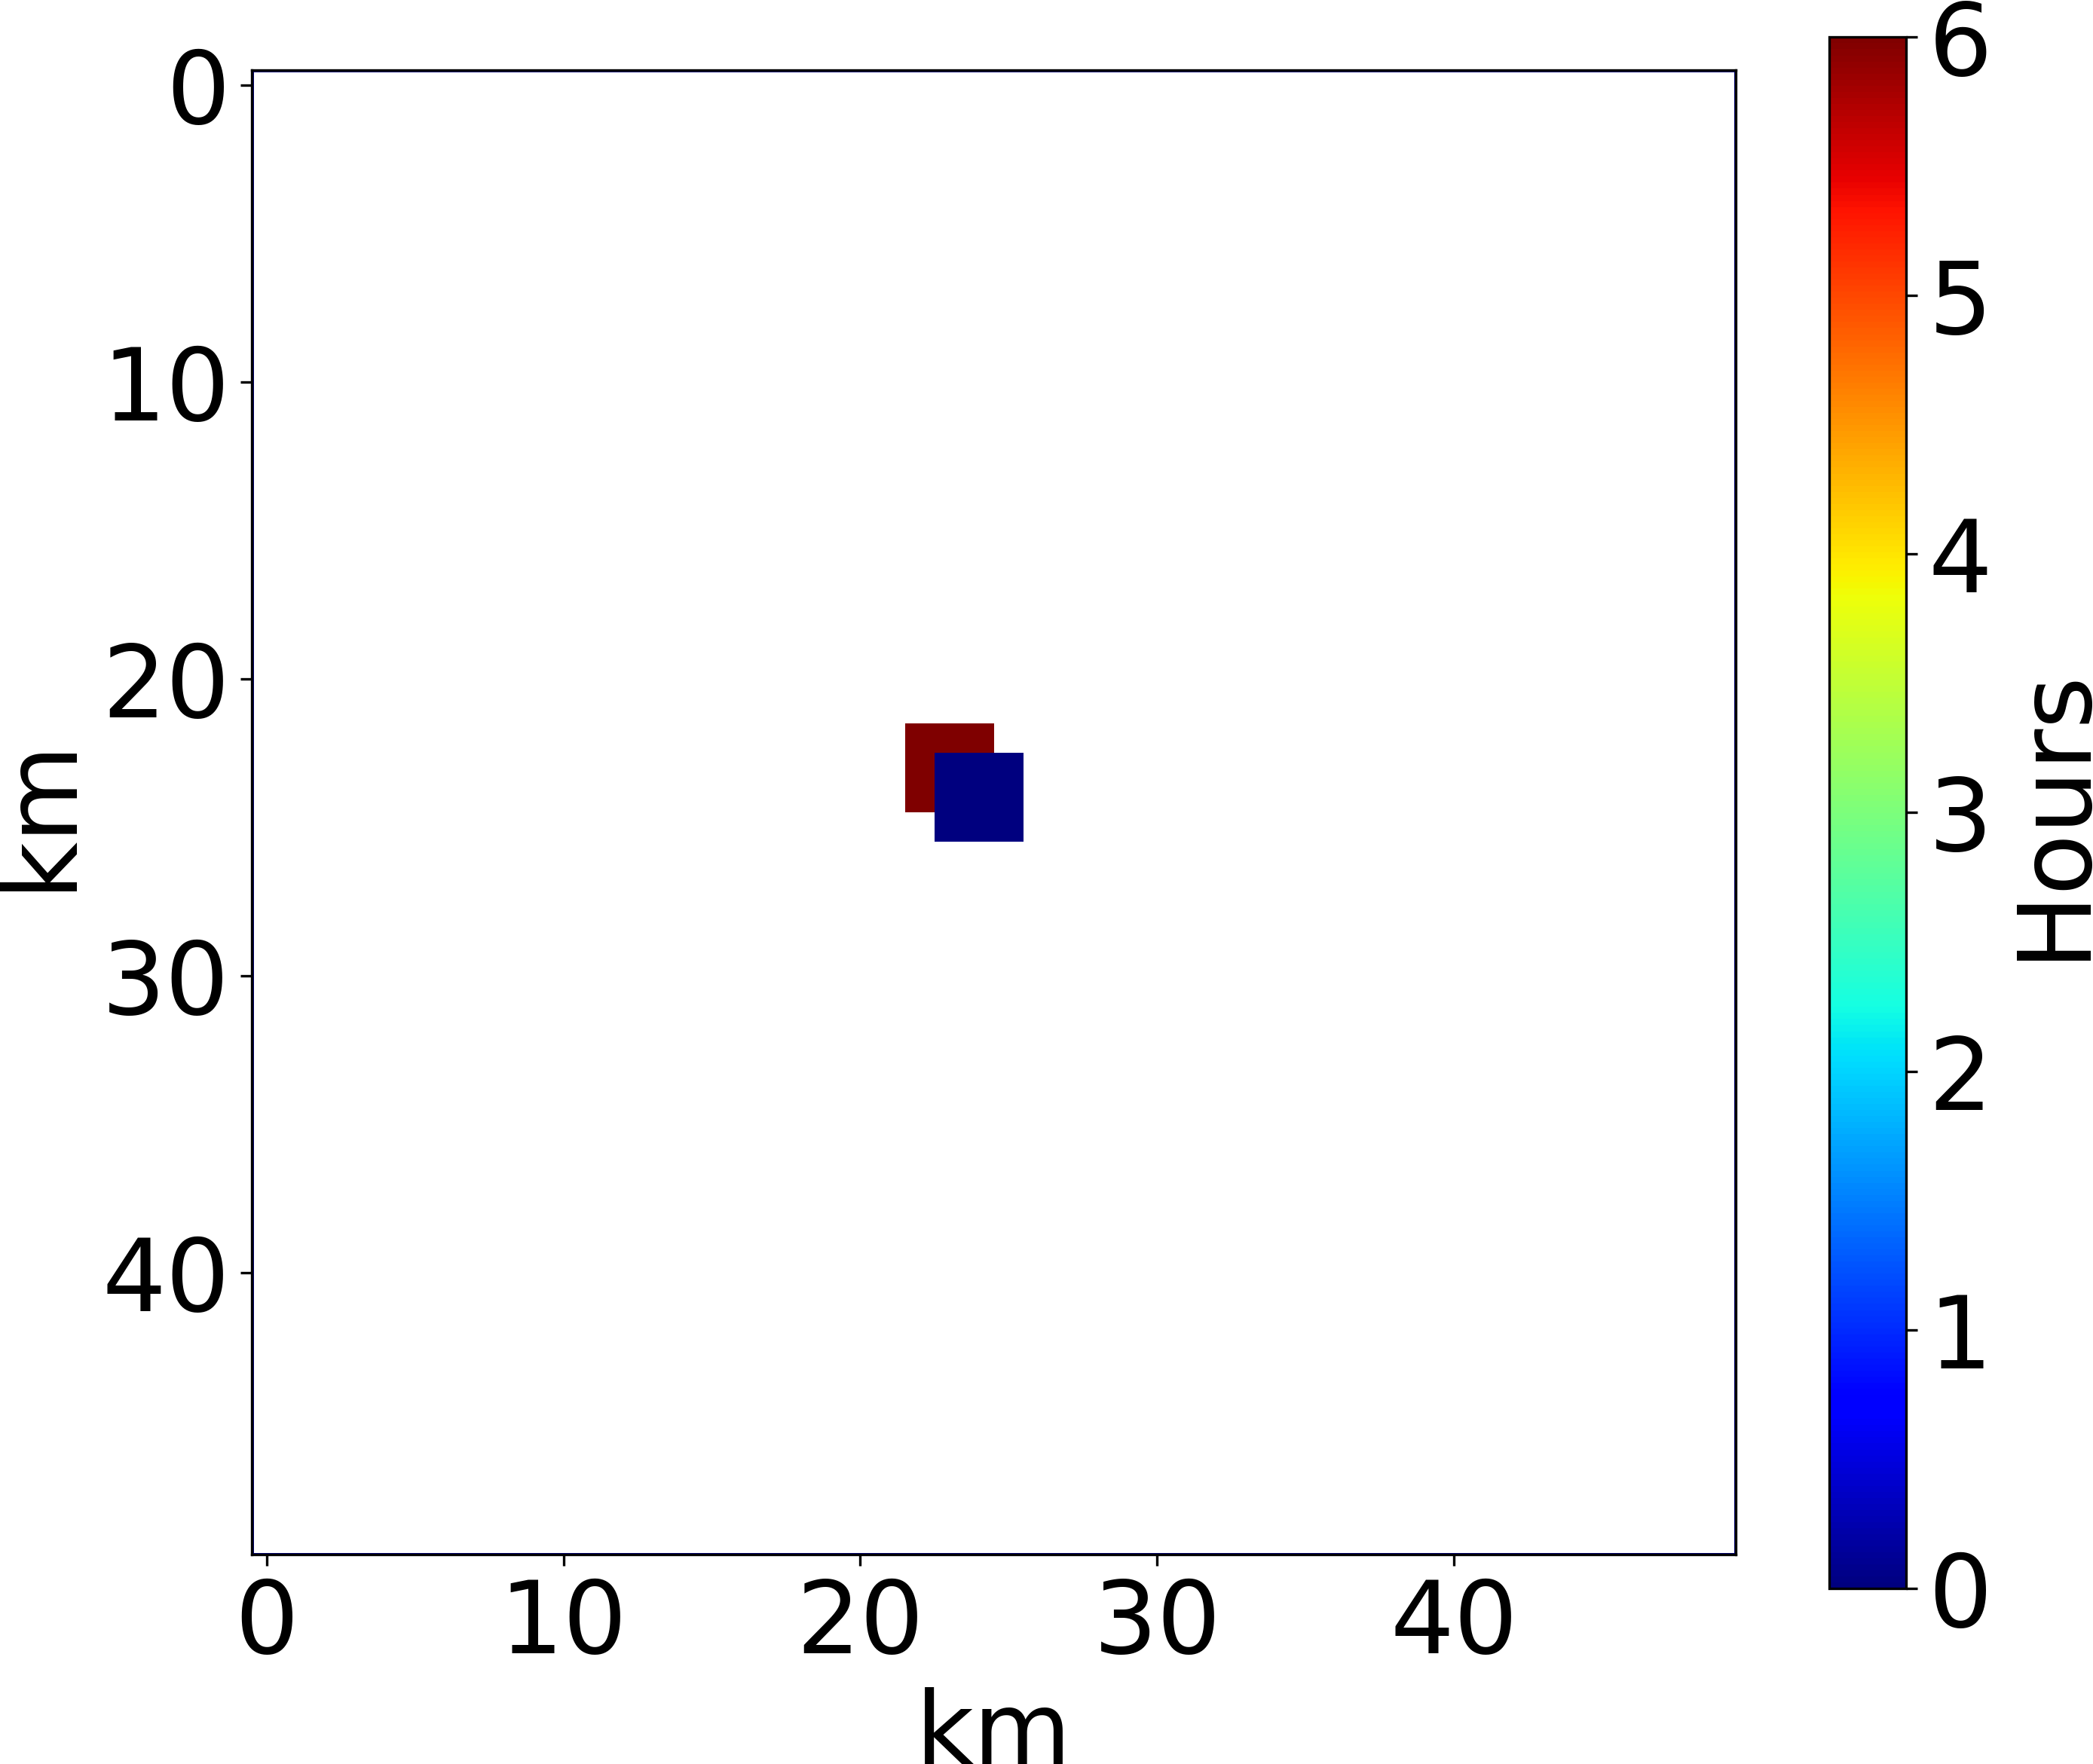
\includegraphics[height=0.25\textwidth]{exampleFusedFire1.png}
	~
	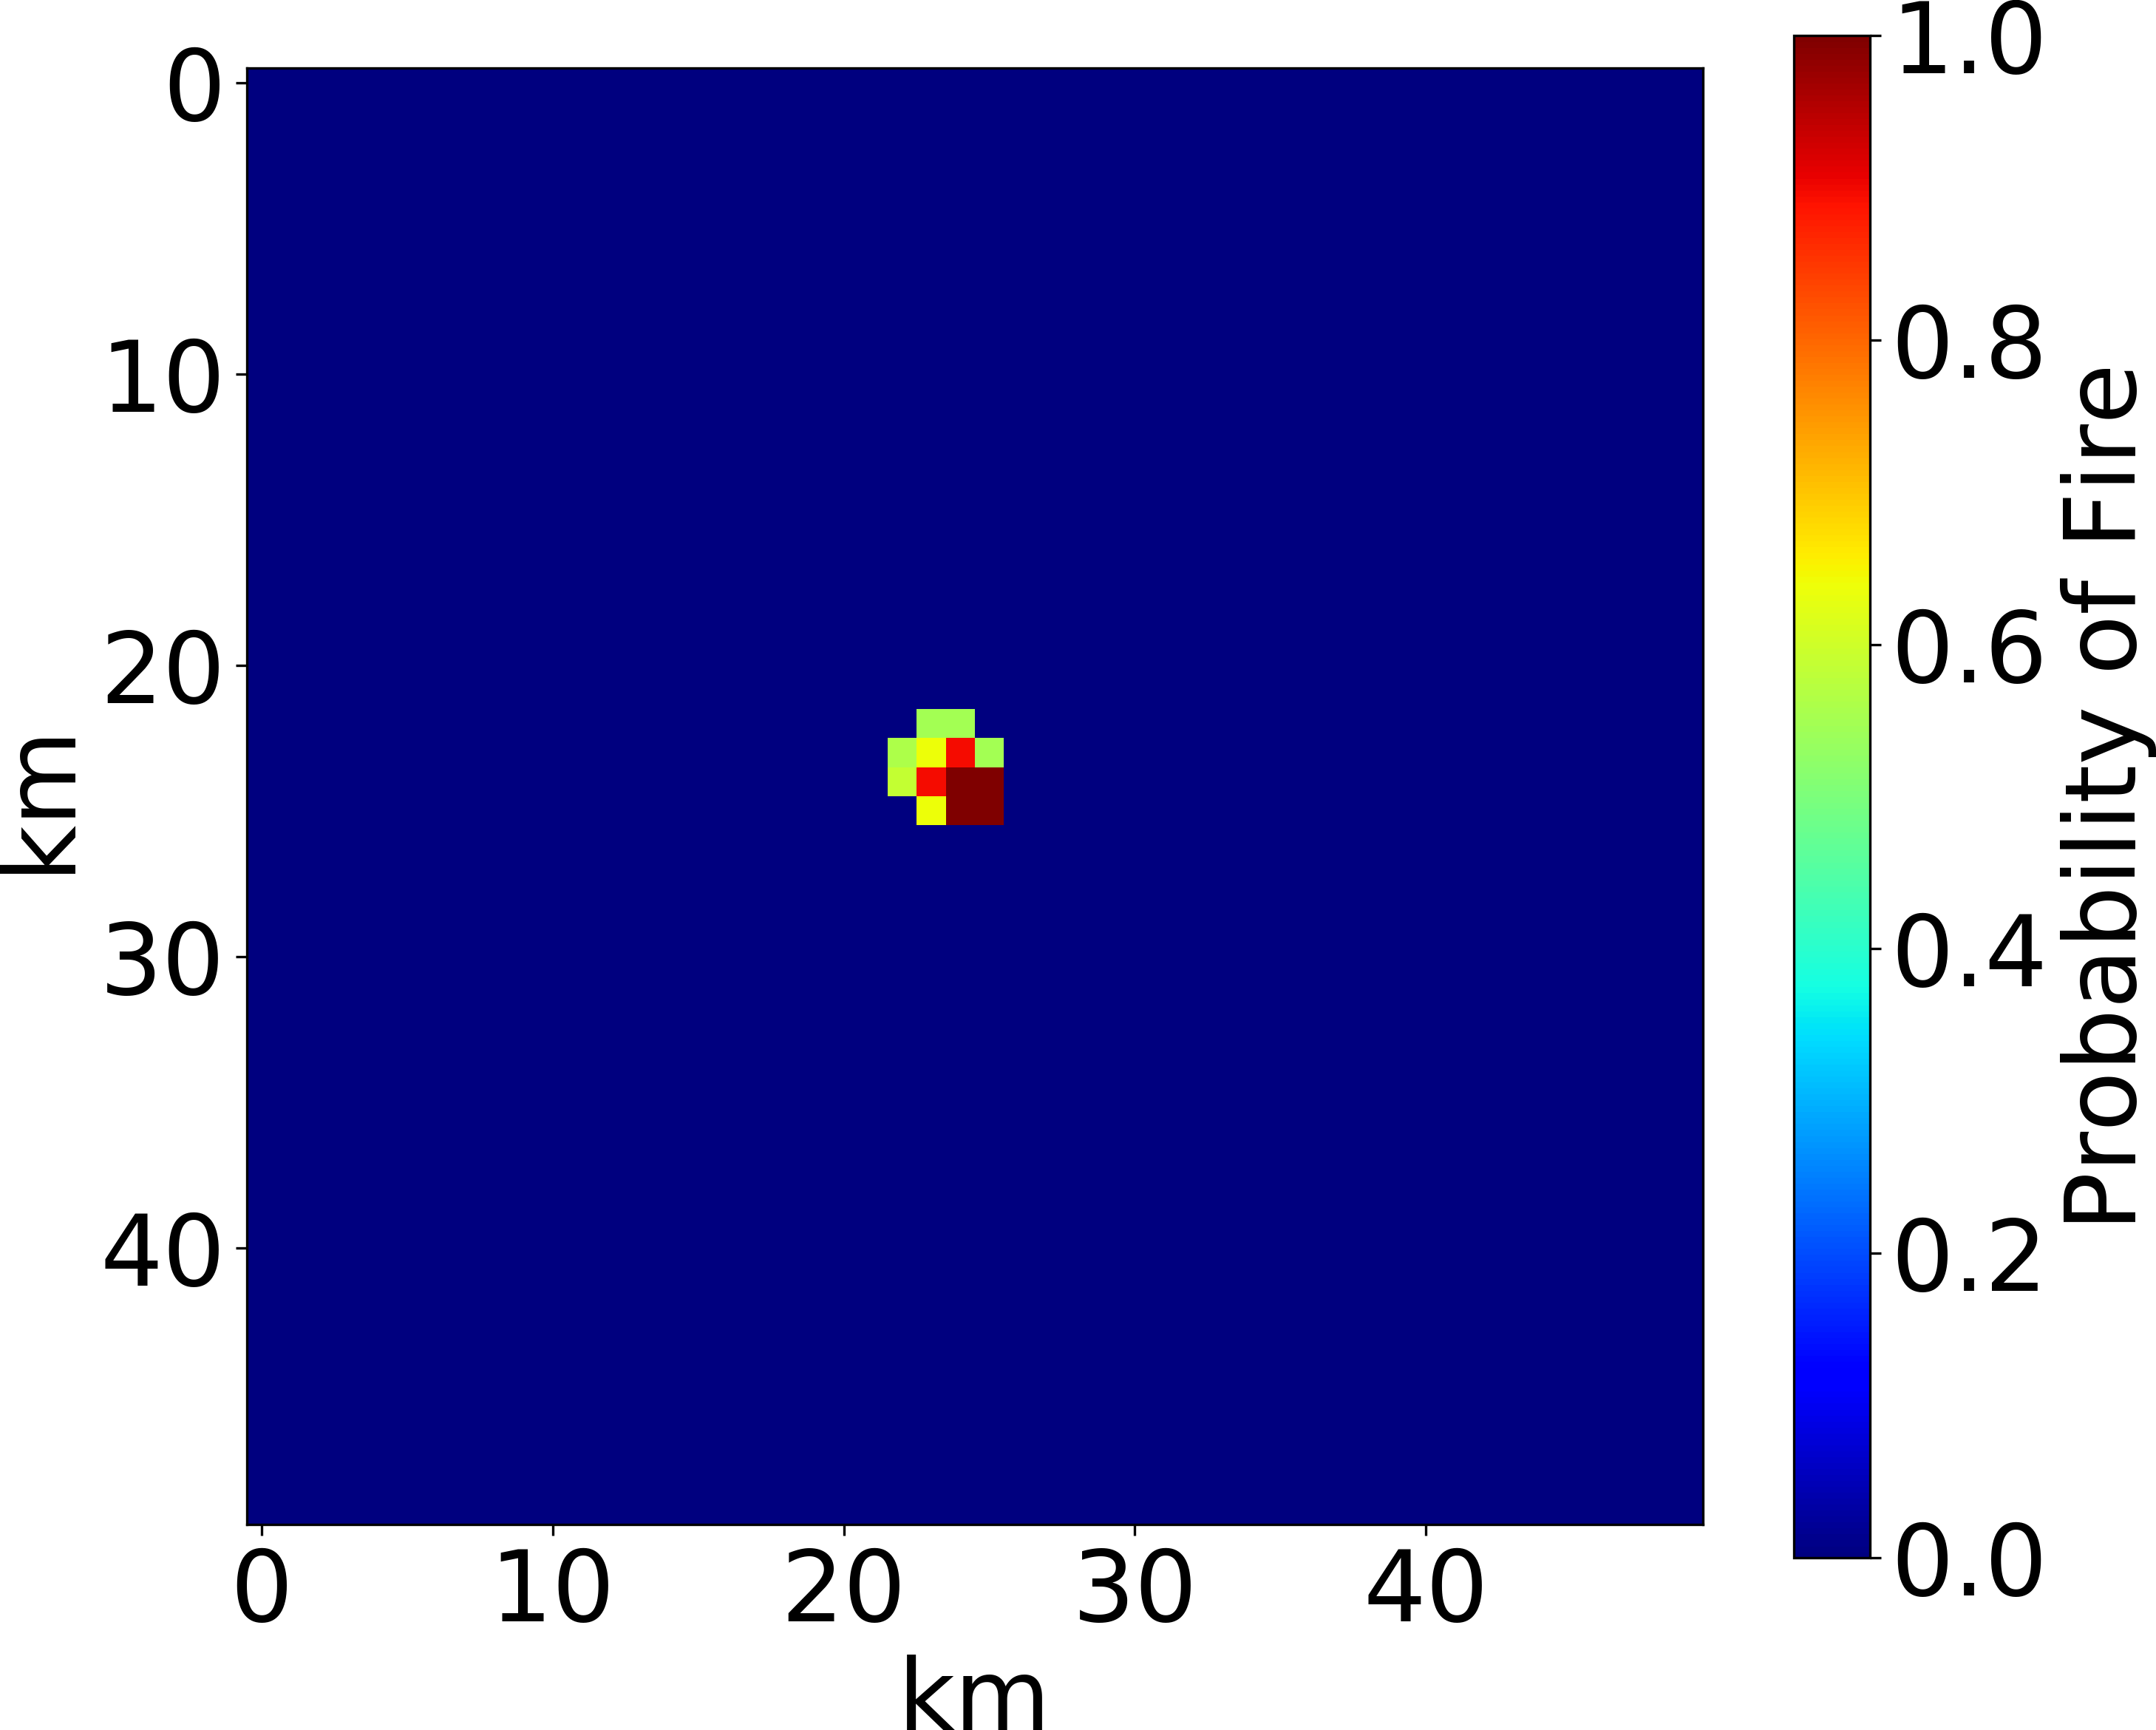
\includegraphics[height=0.25\textwidth]{exampleNetworkProcessed1.png}
	~
	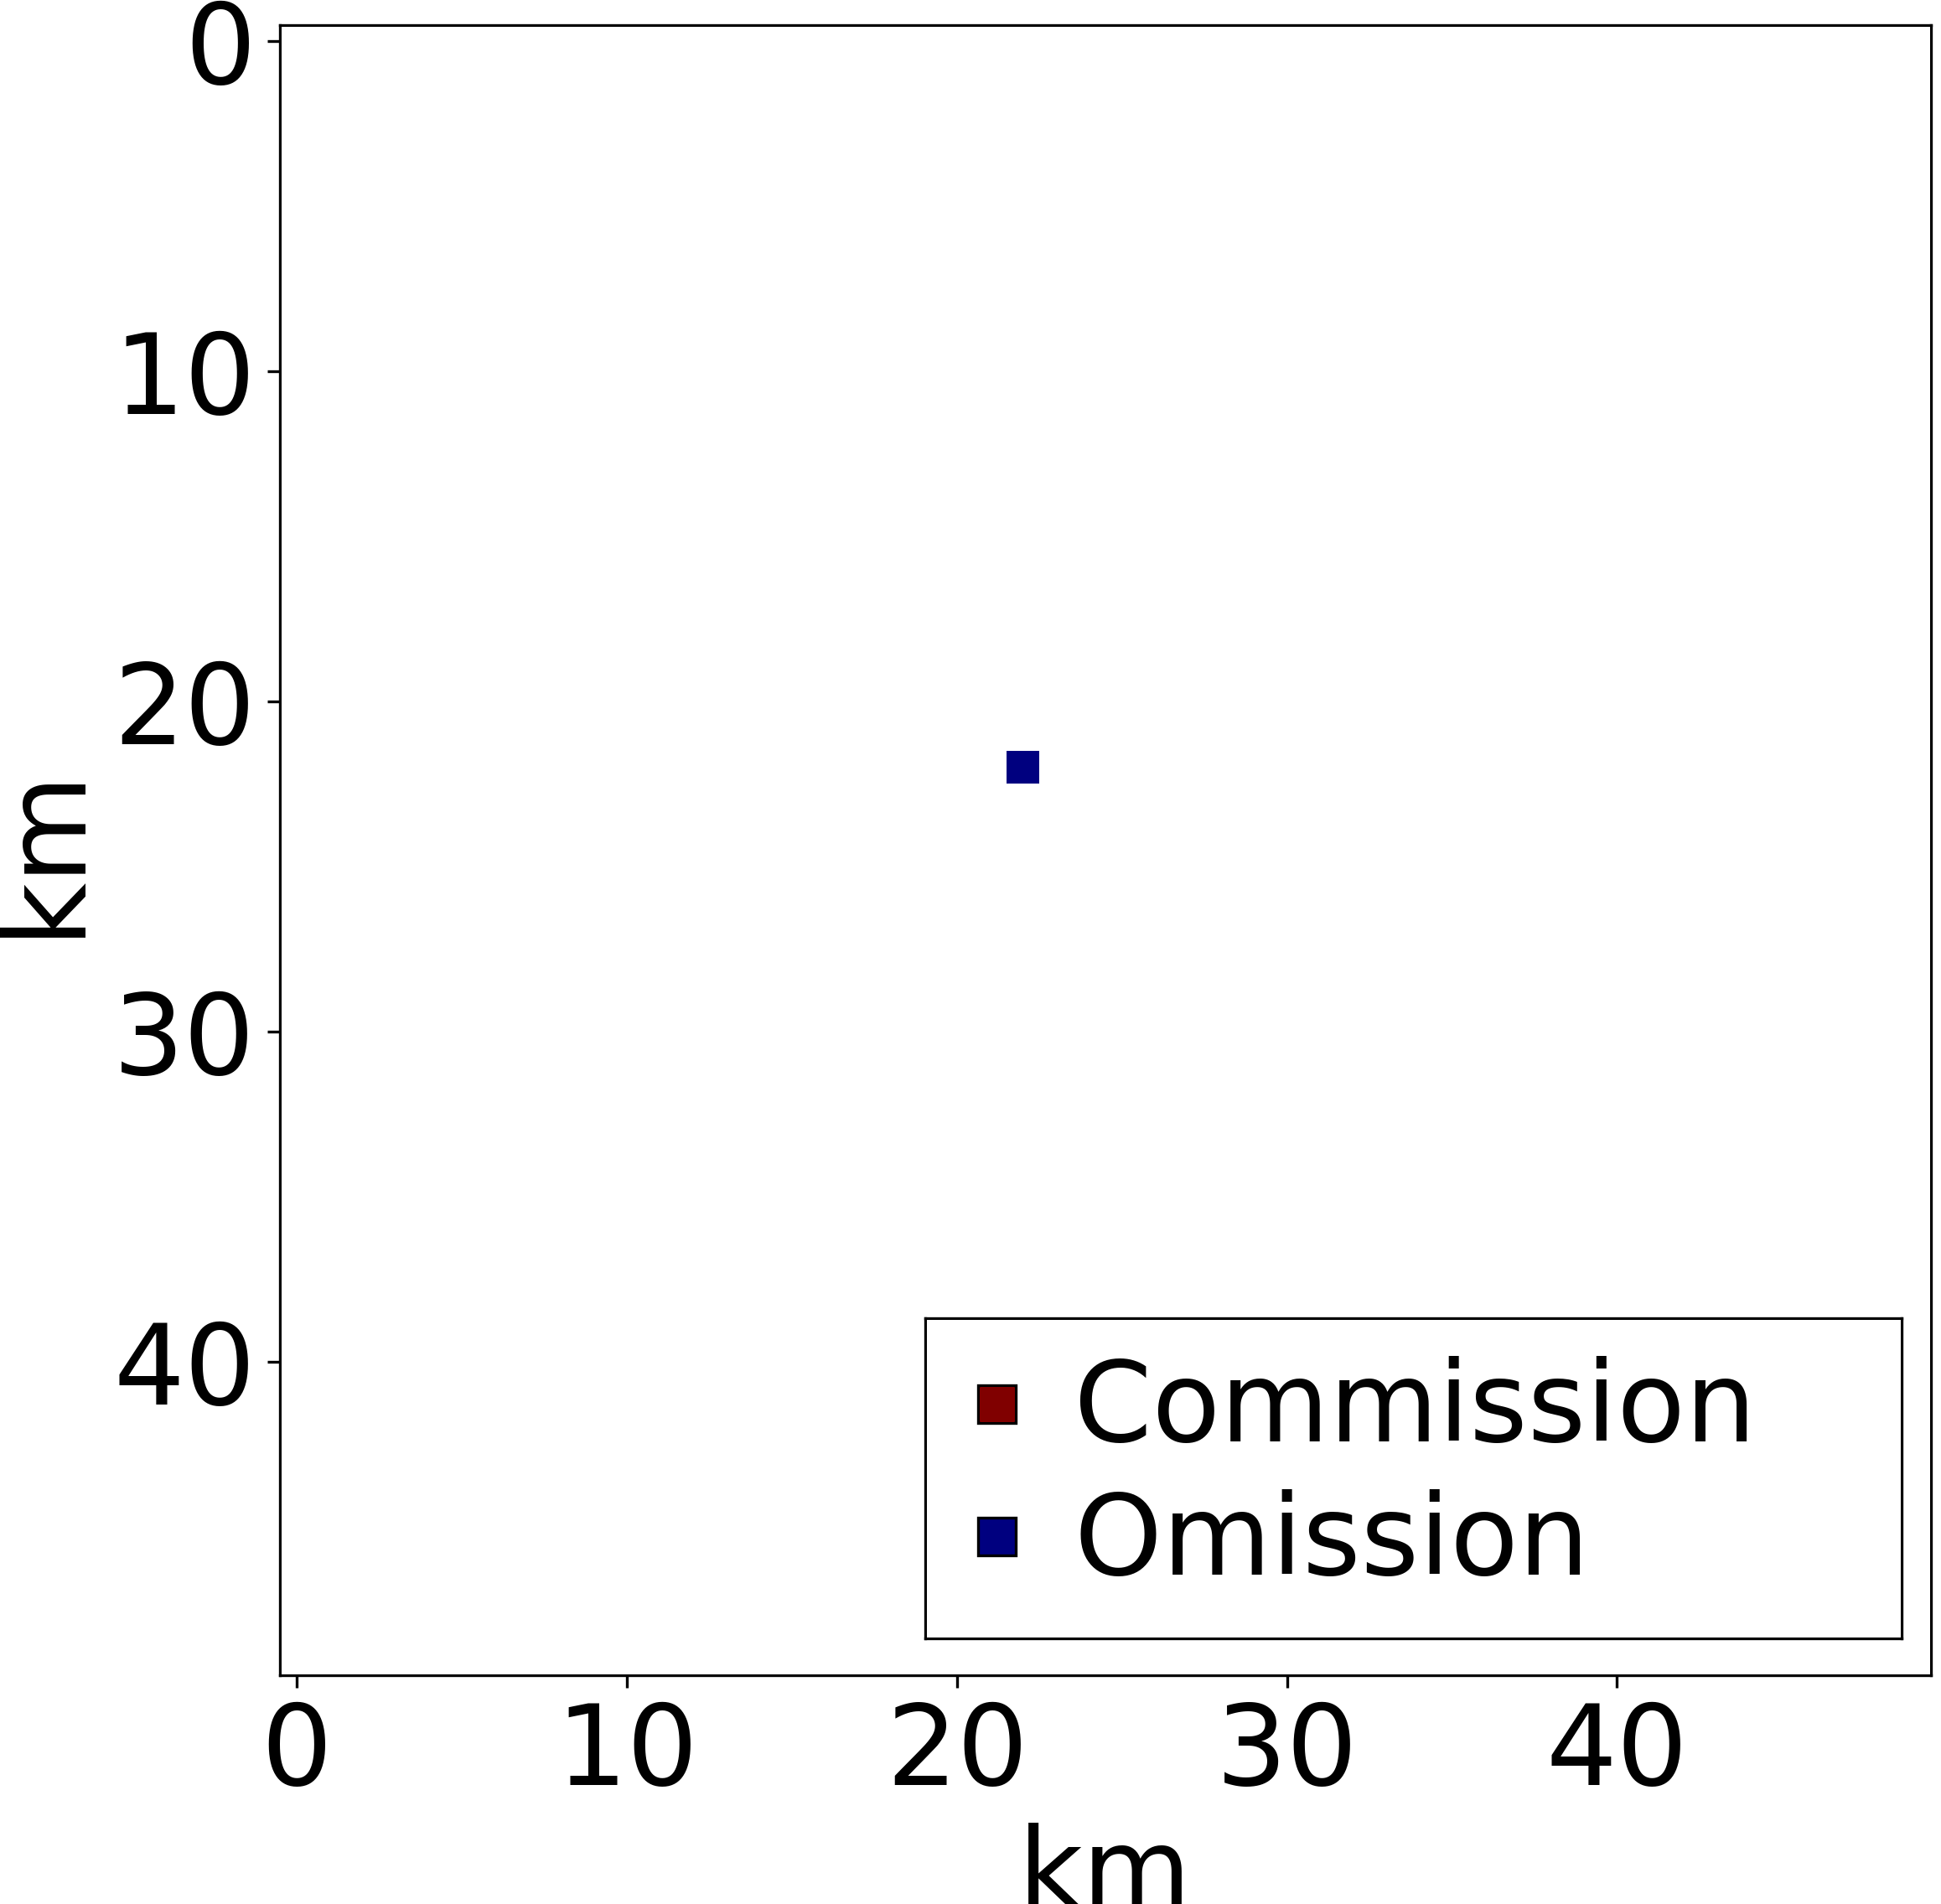
\includegraphics[height=0.25\textwidth]{exampleNetworkError1.png}
	\\
	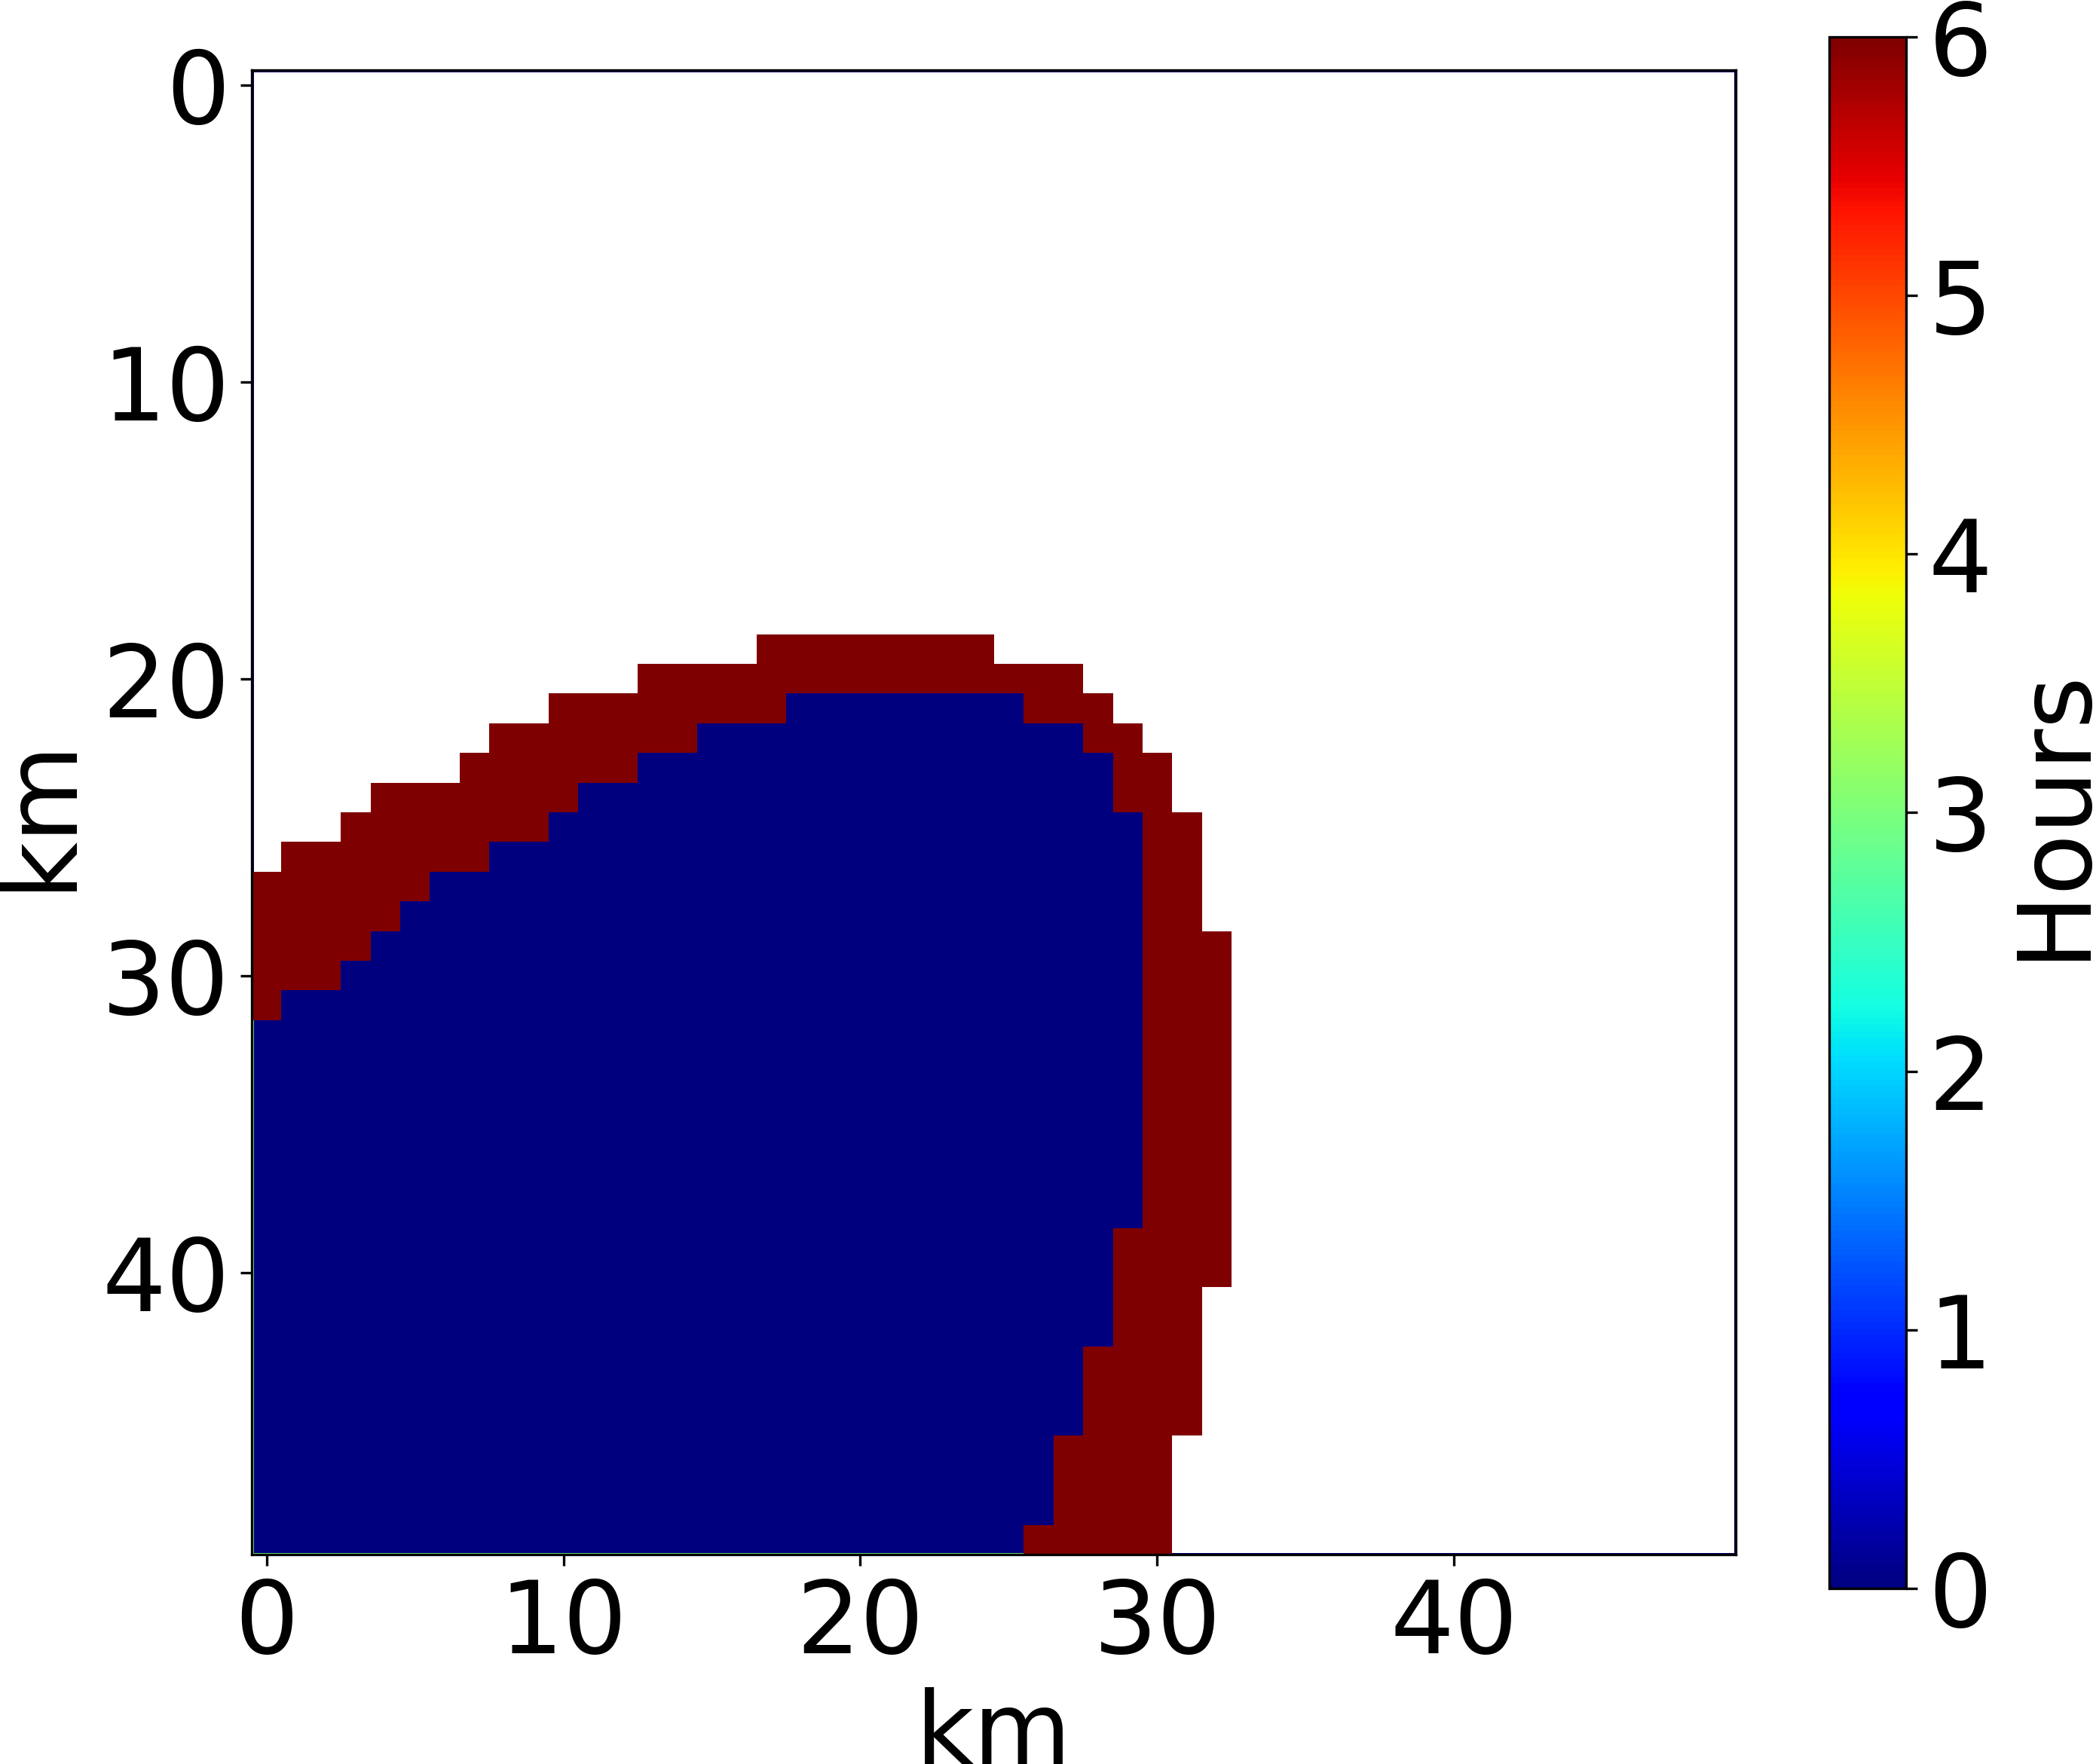
\includegraphics[height=0.25\textwidth]{exampleFusedFire2.png}
	~
	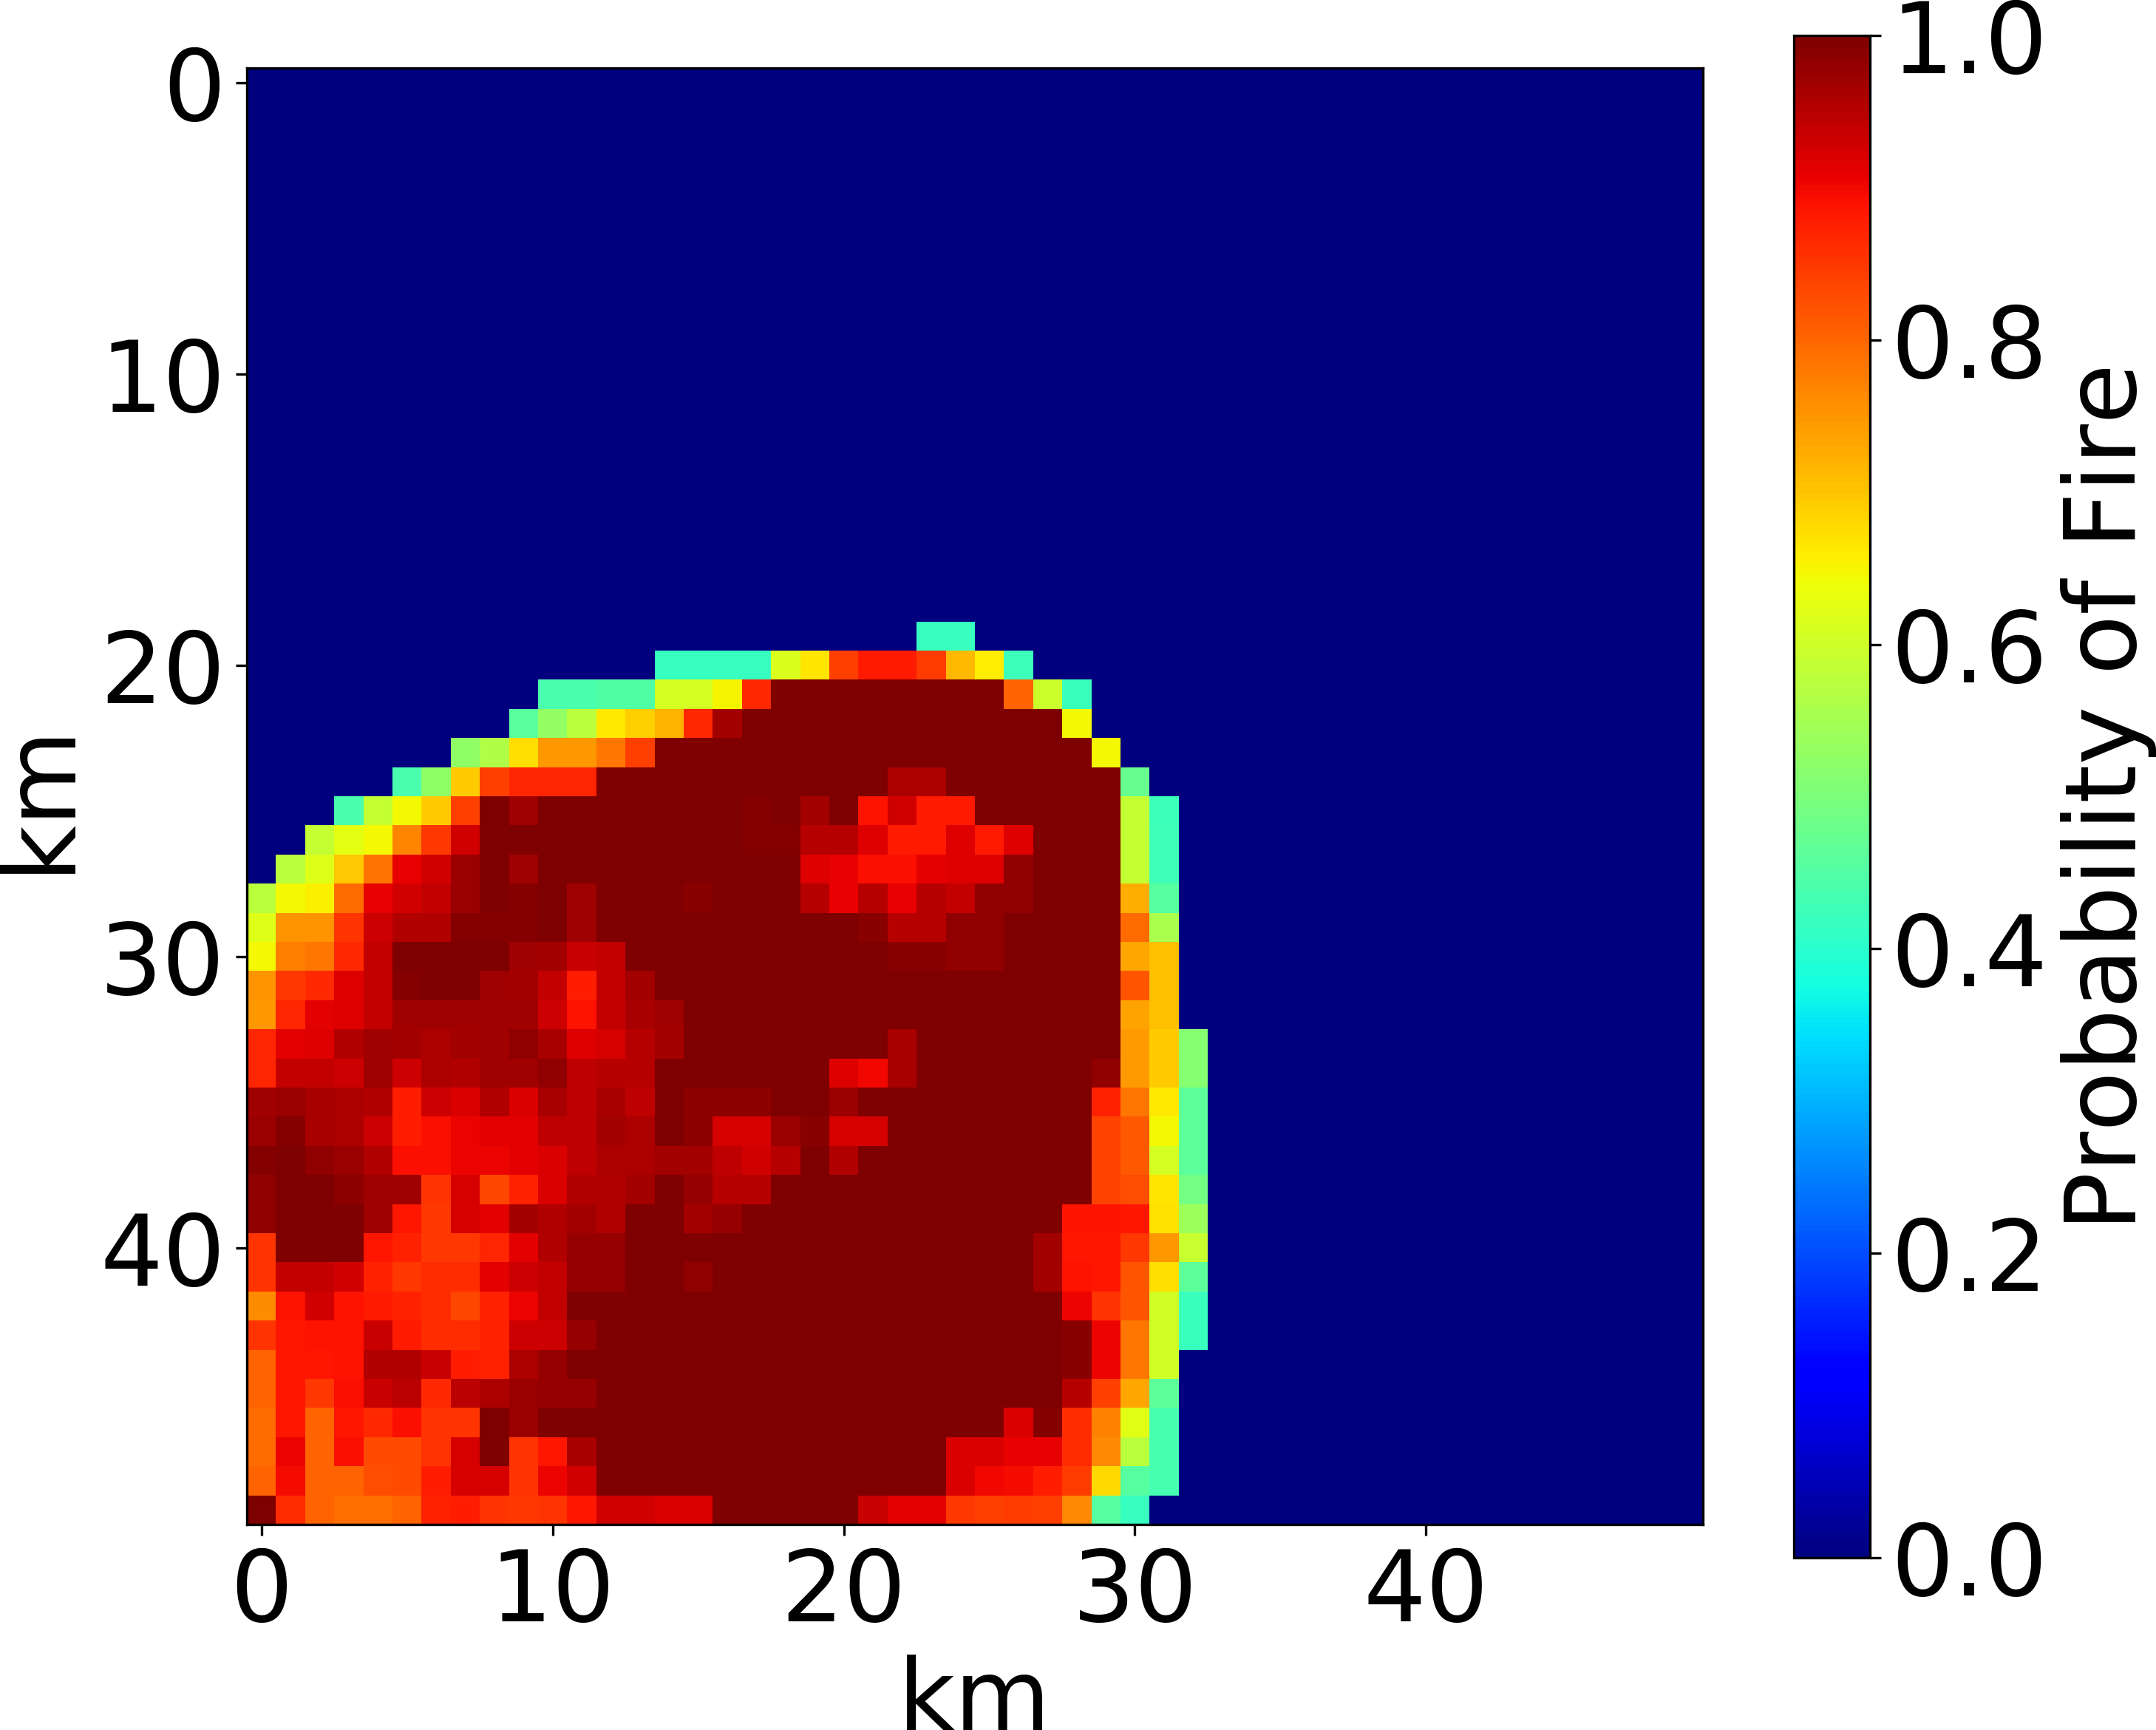
\includegraphics[height=0.25\textwidth]{exampleNetworkProcessed2.png}
	~
	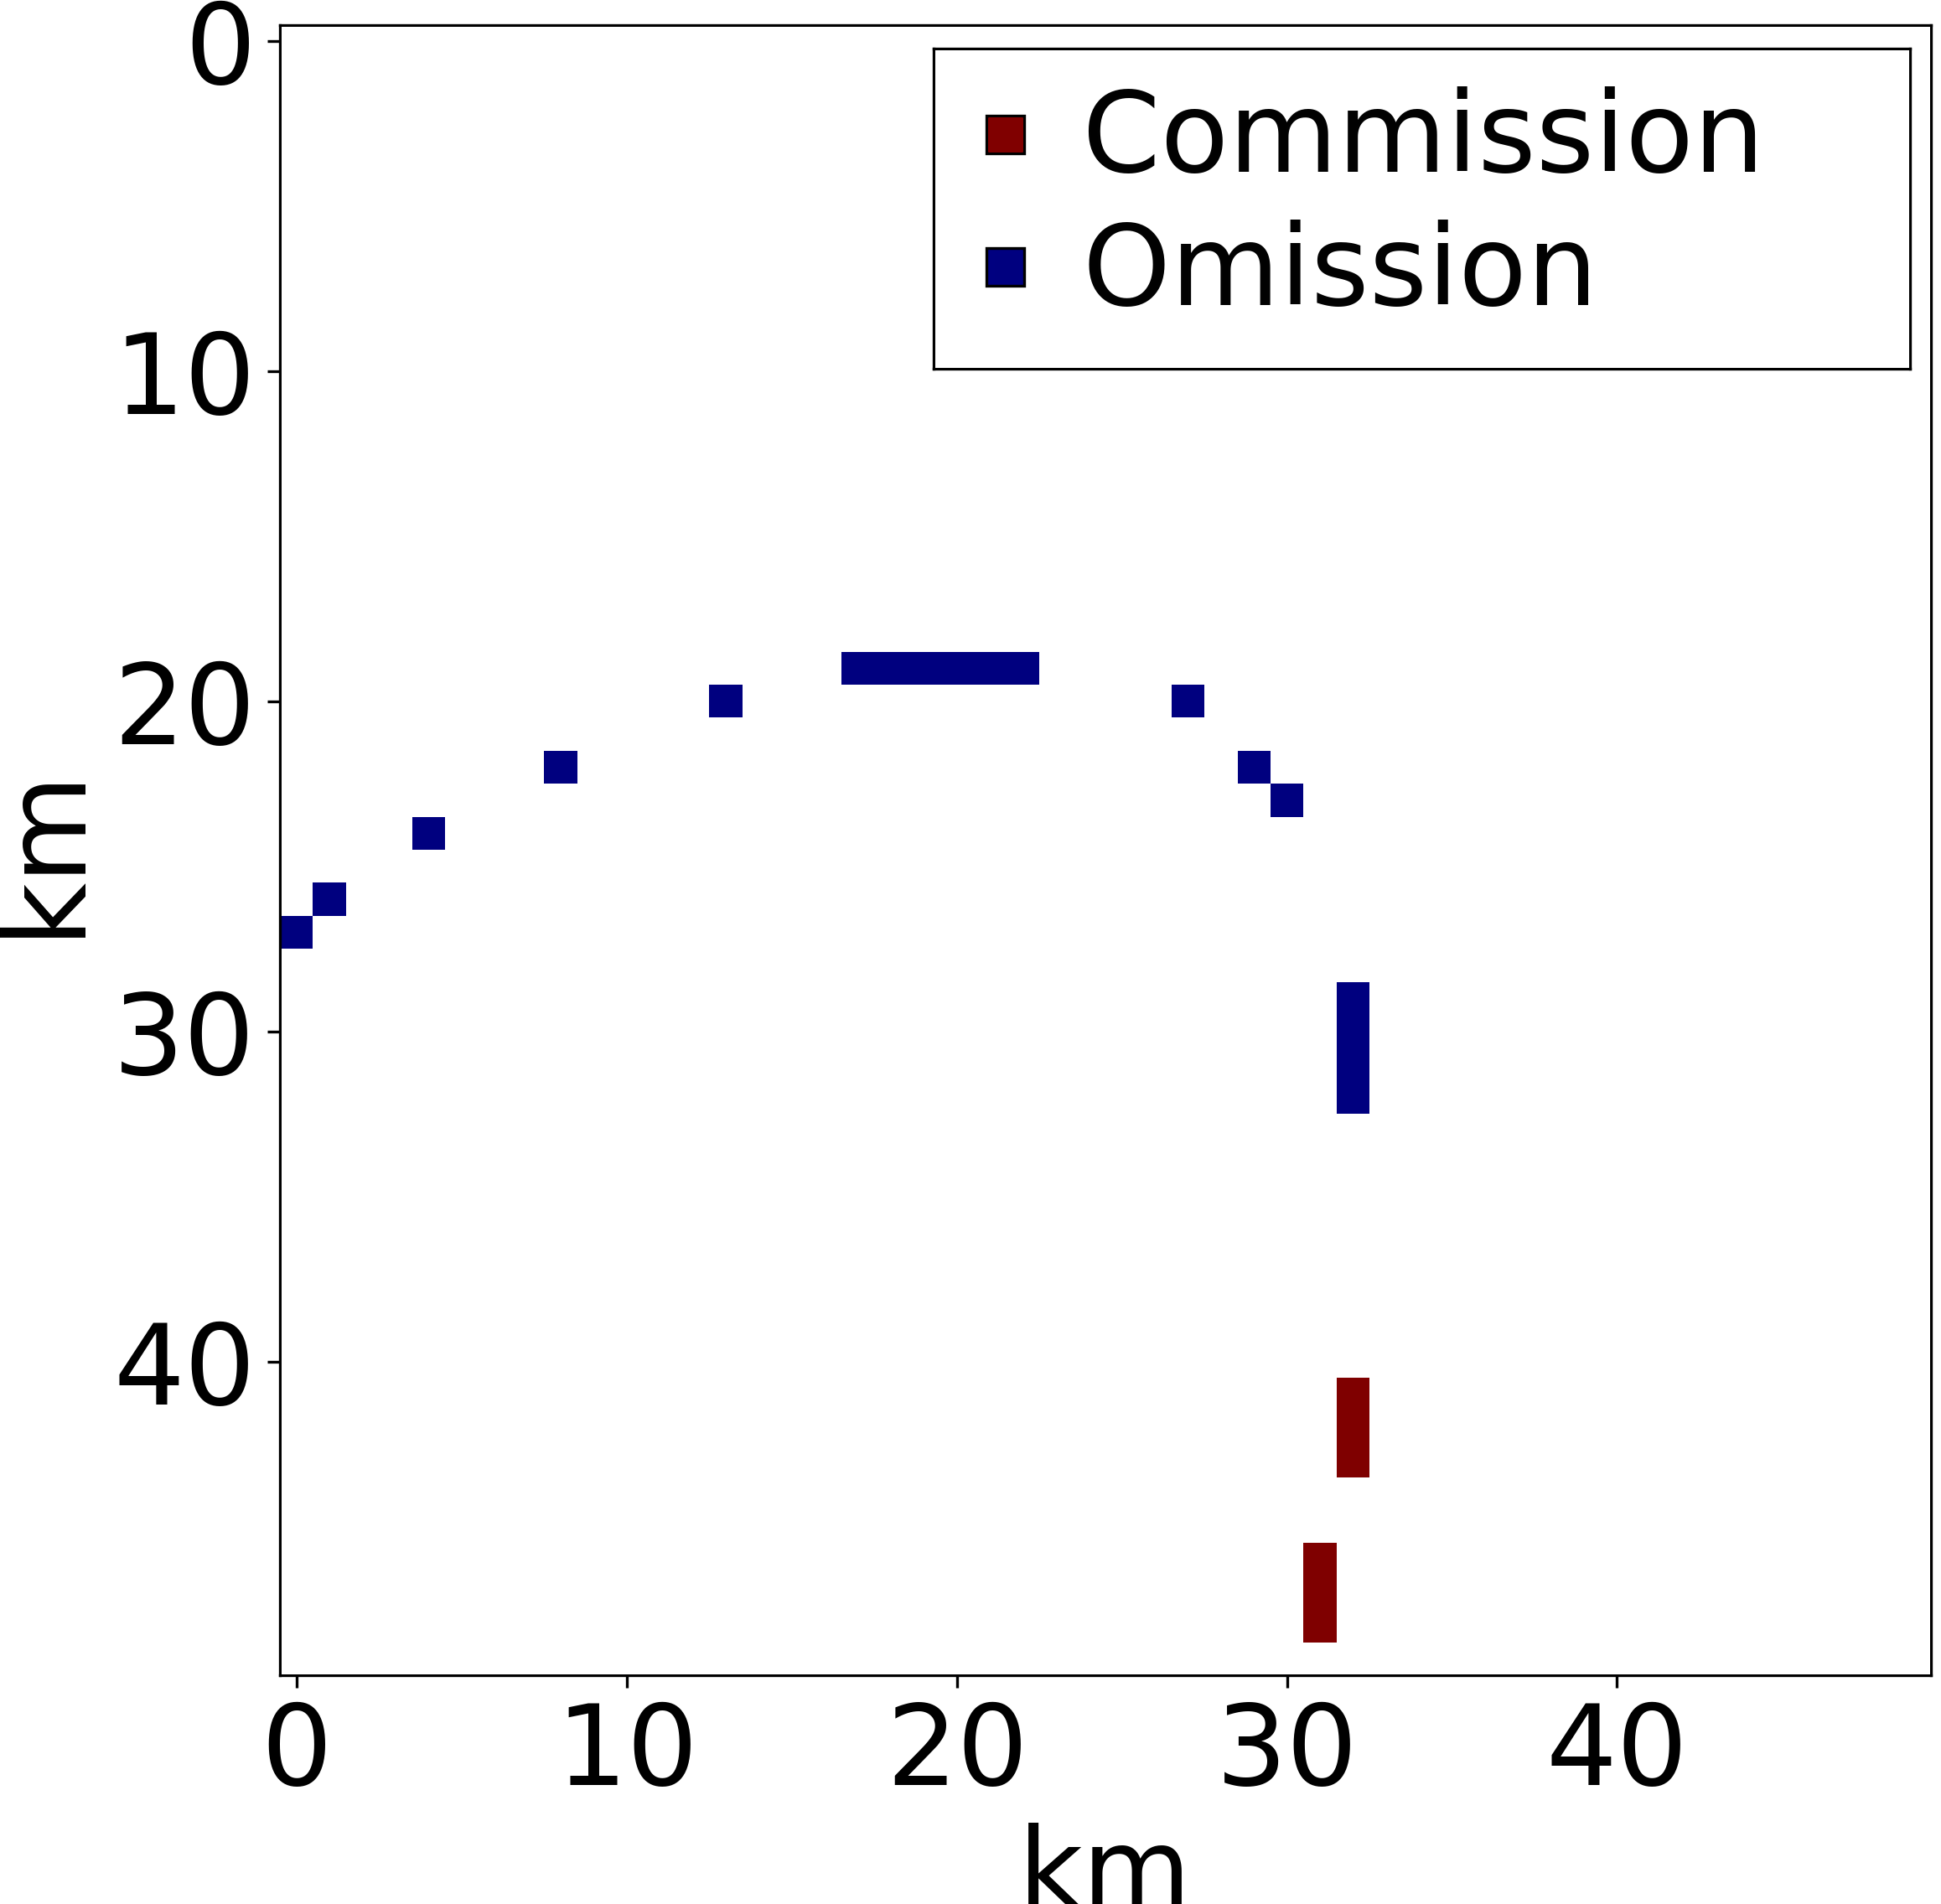
\includegraphics[height=0.25\textwidth]{exampleNetworkError2.png}
	\\
	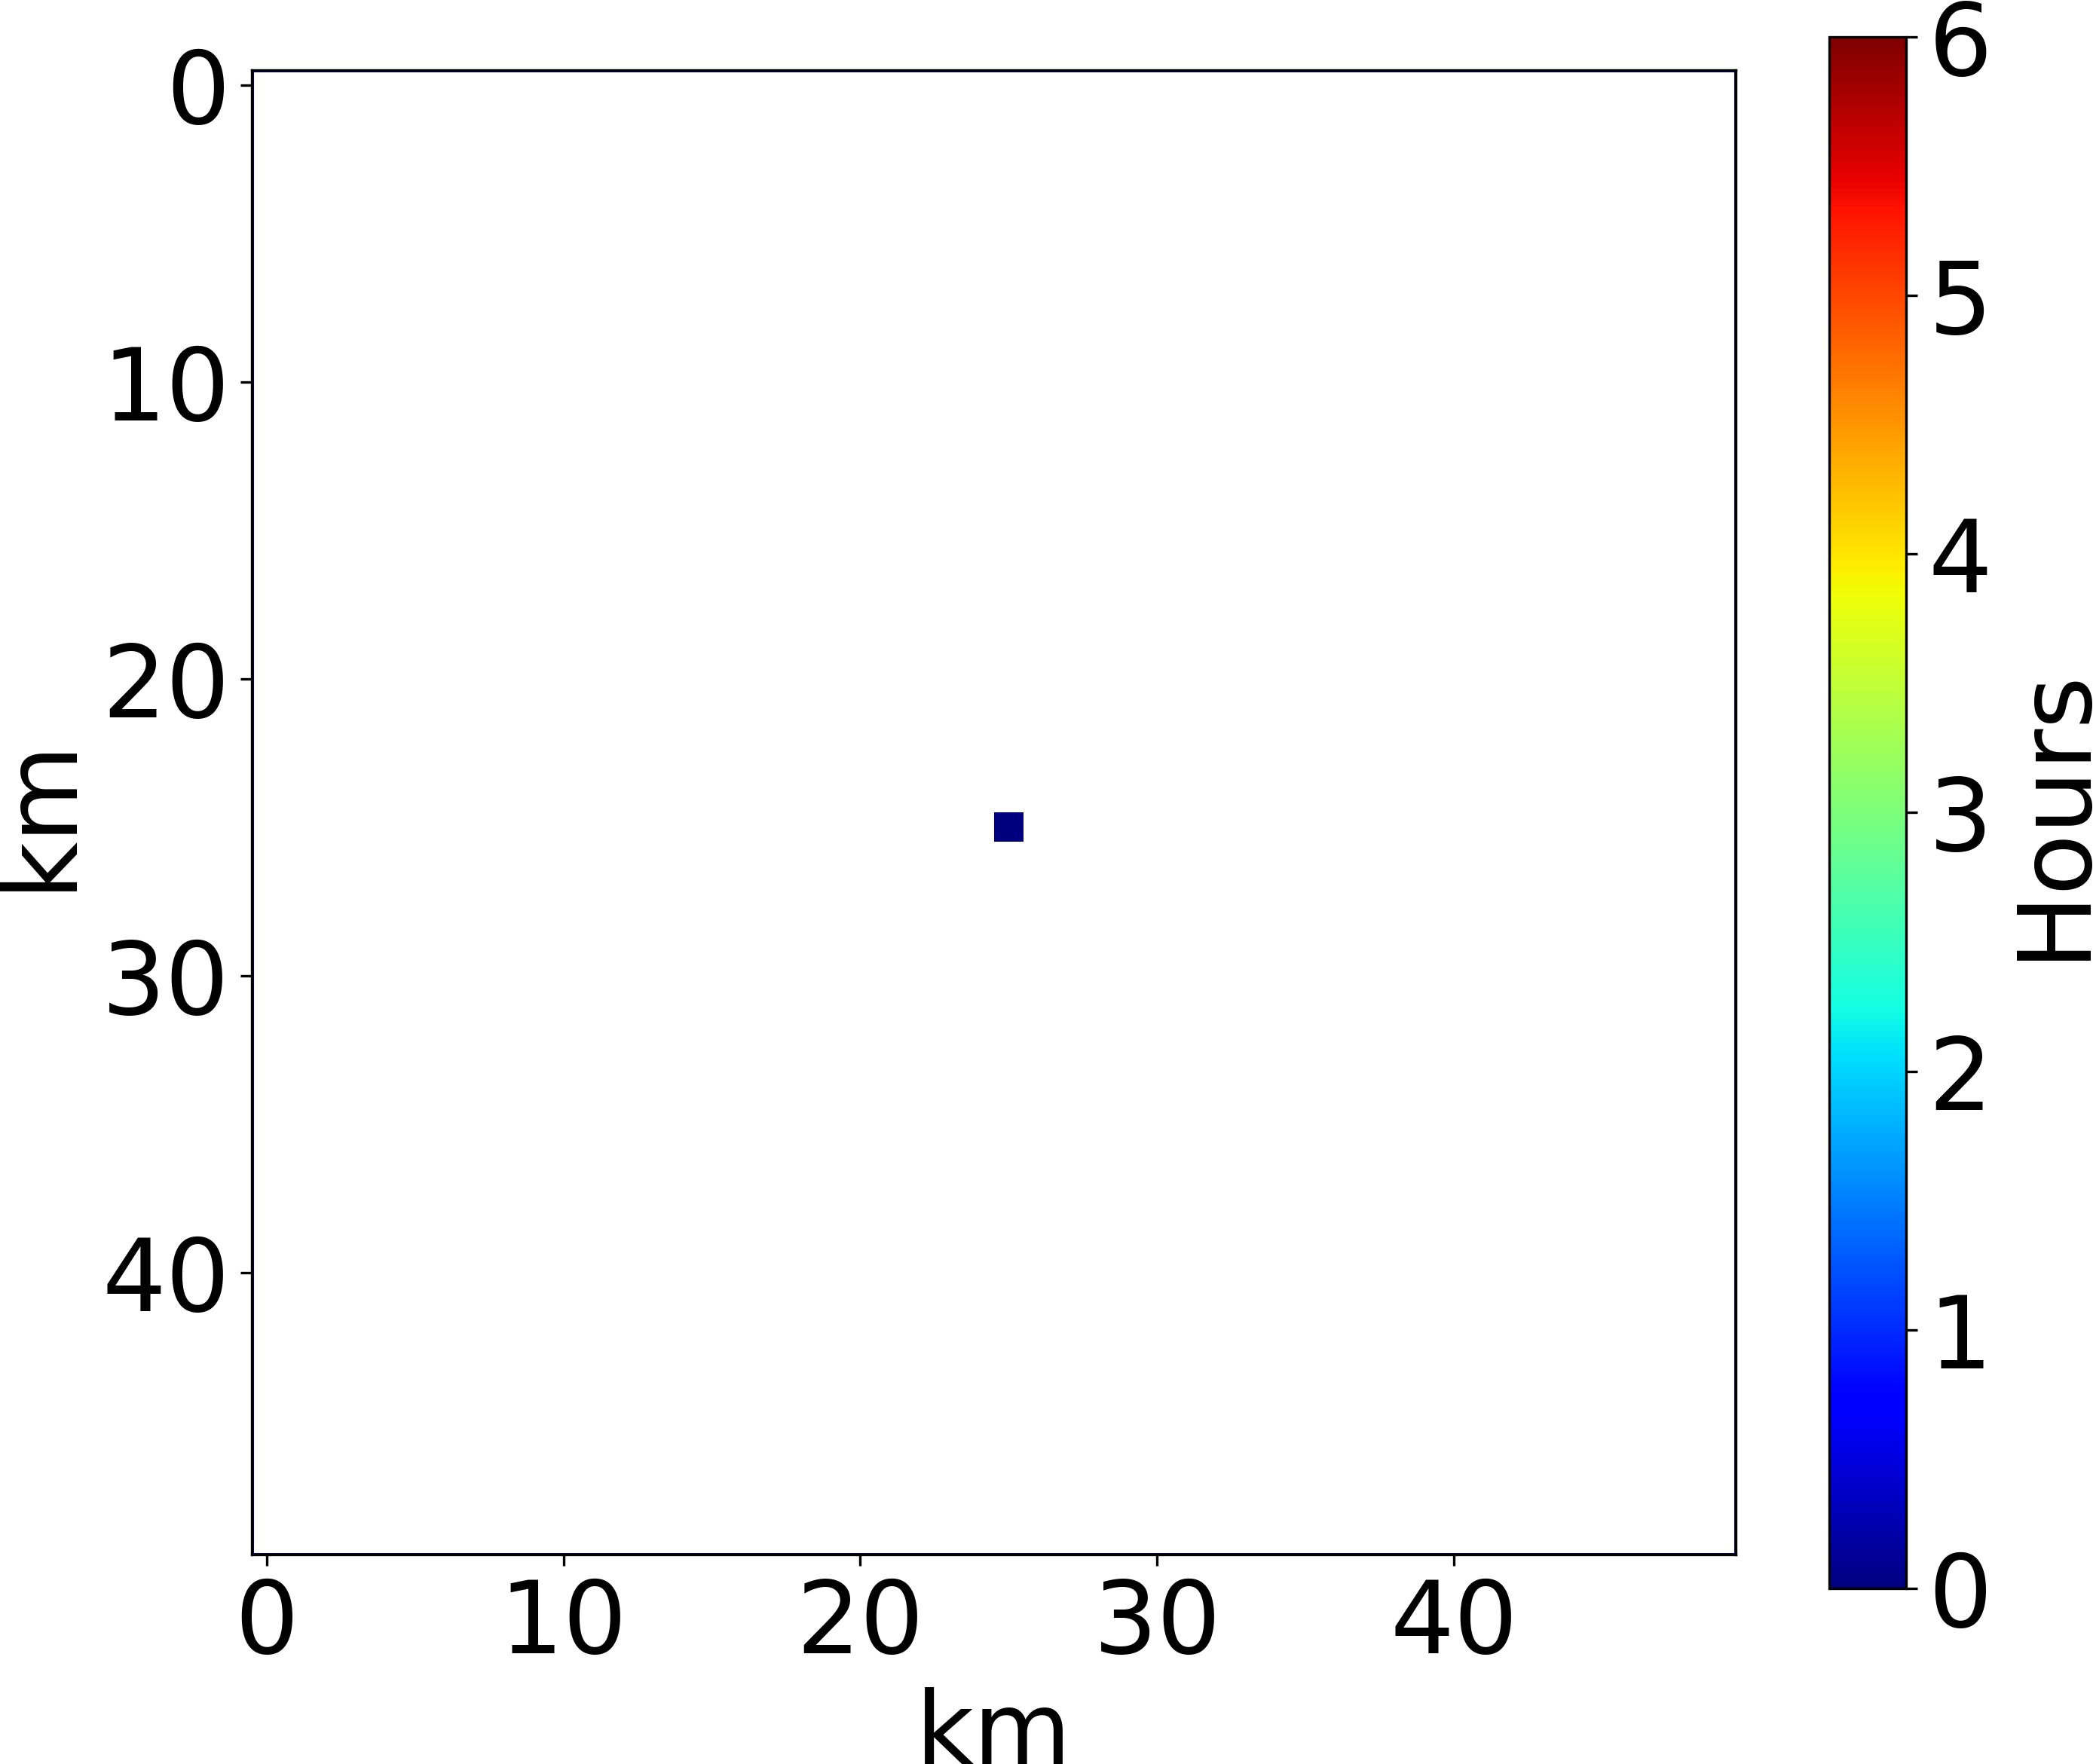
\includegraphics[height=0.25\textwidth]{exampleFusedFire3.png}
	~
	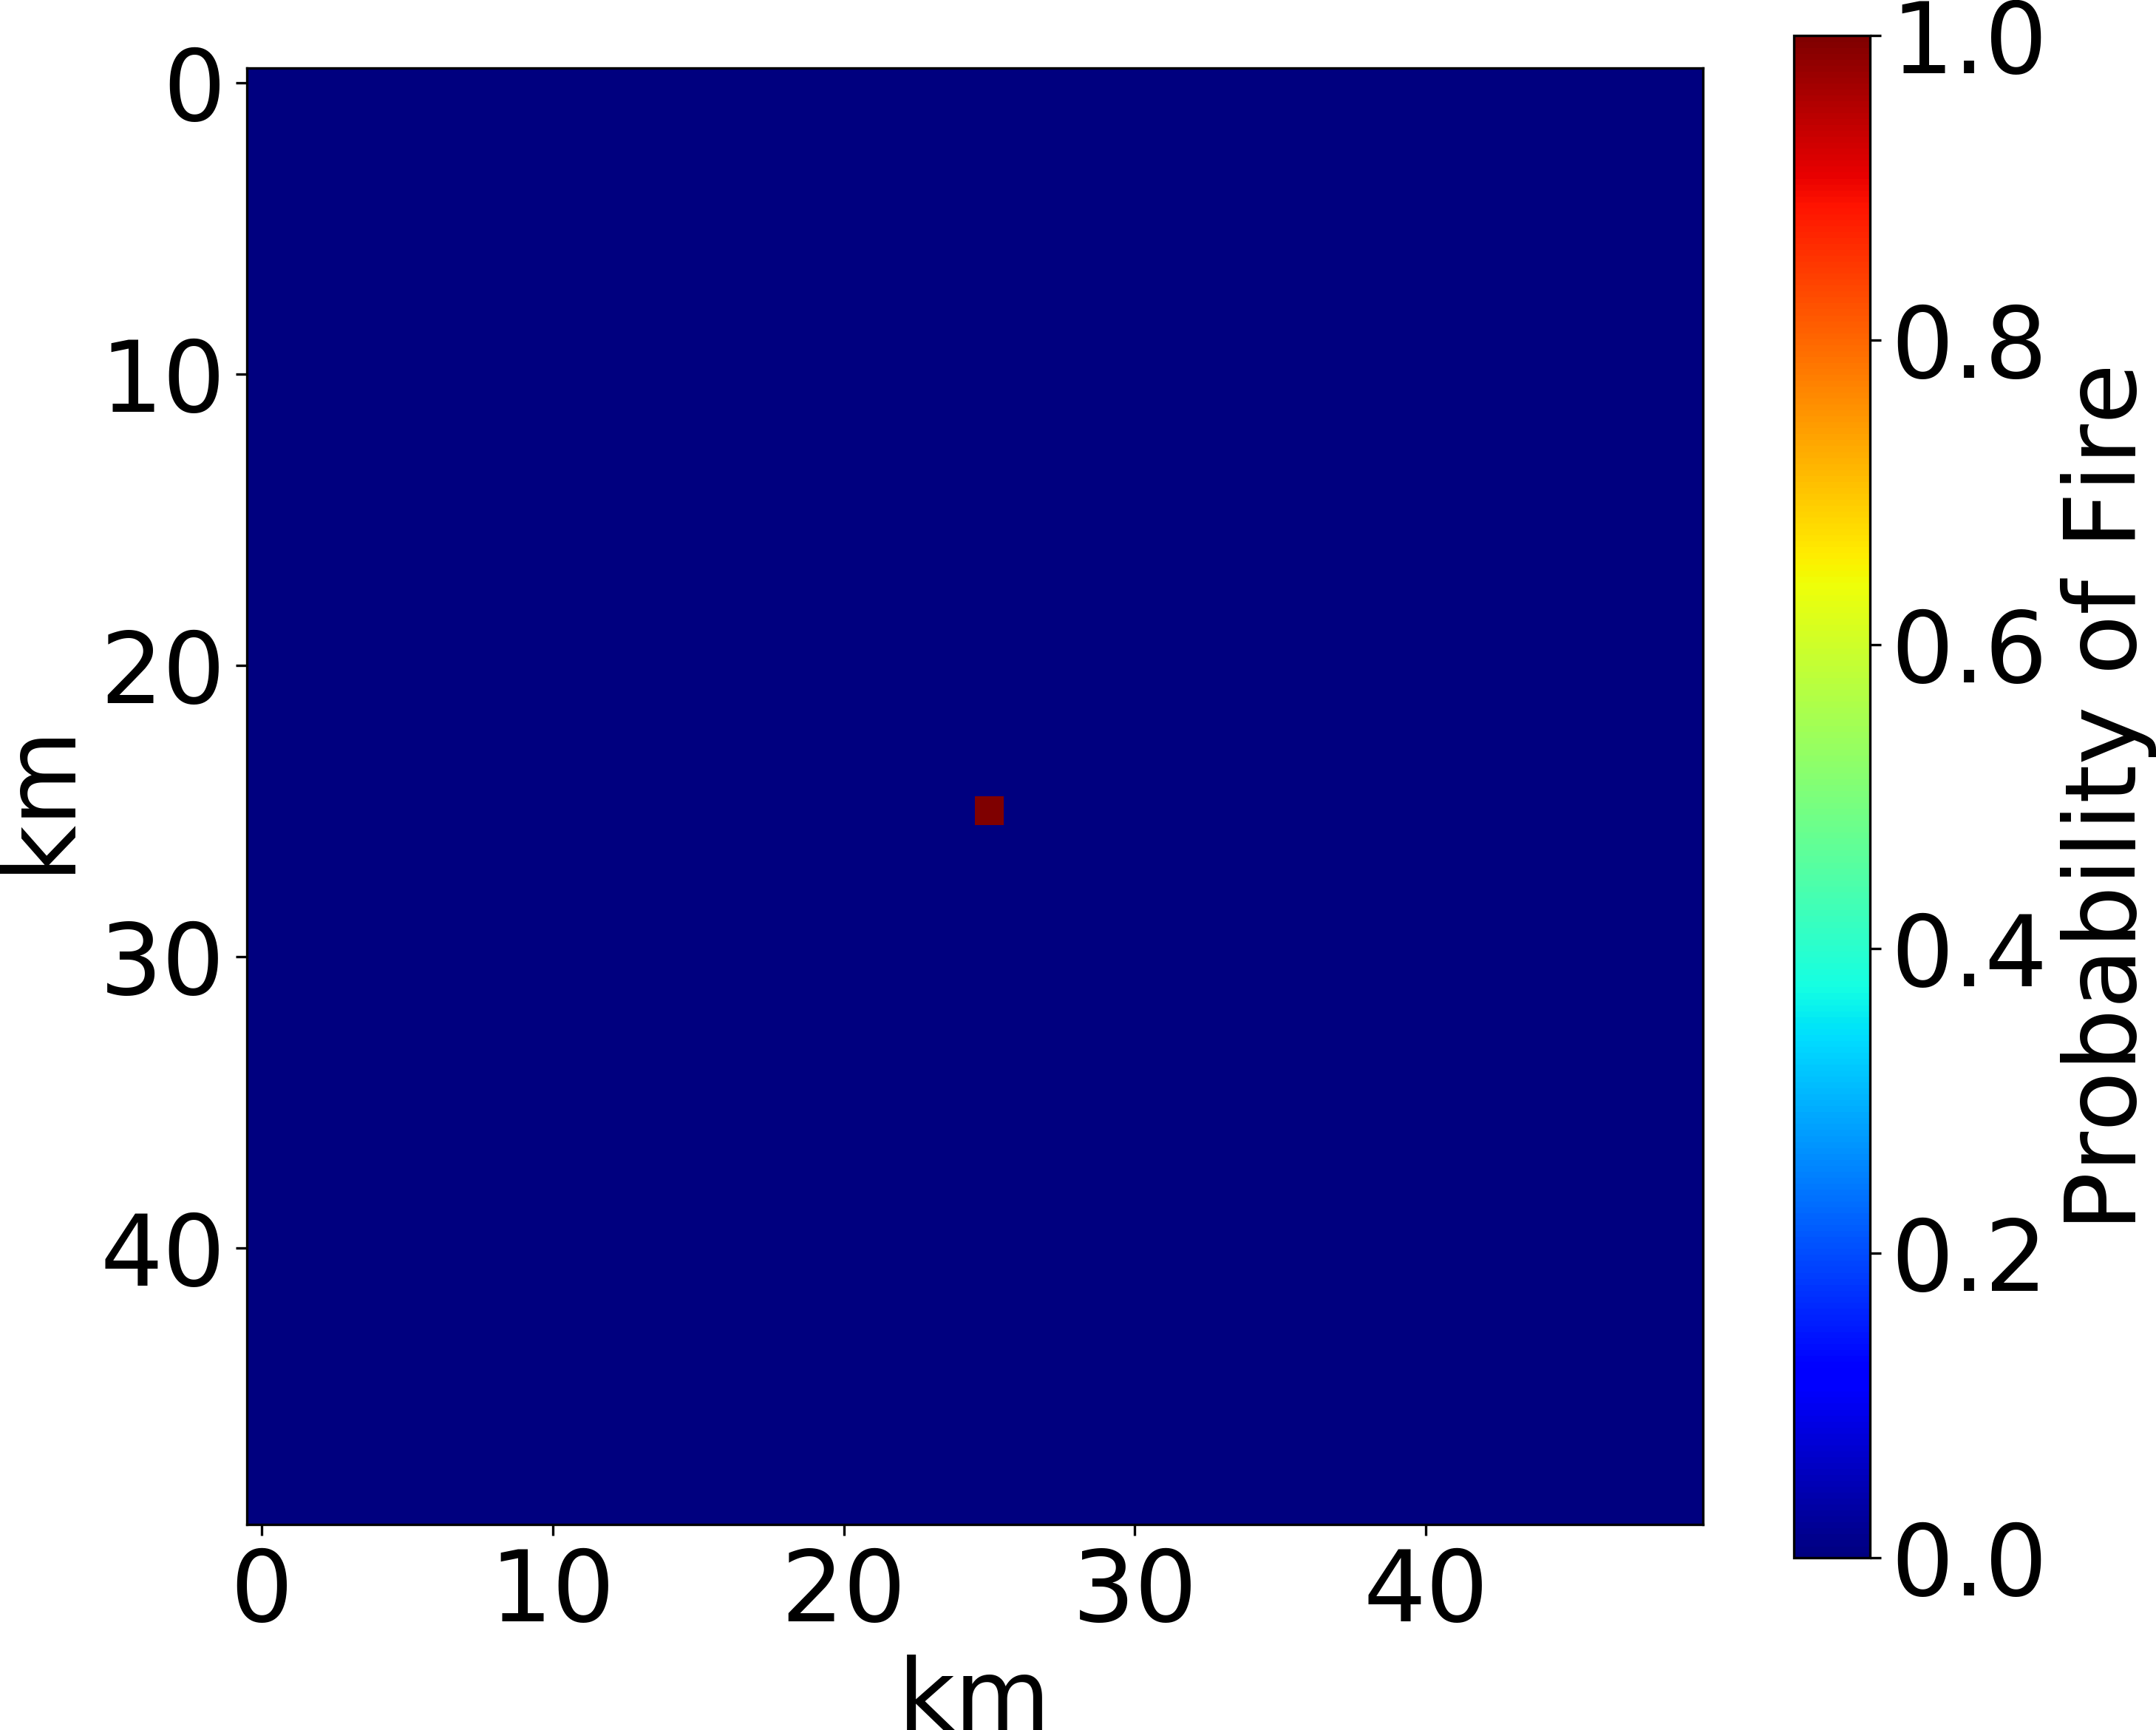
\includegraphics[height=0.25\textwidth]{exampleNetworkProcessed3.png}
	~
	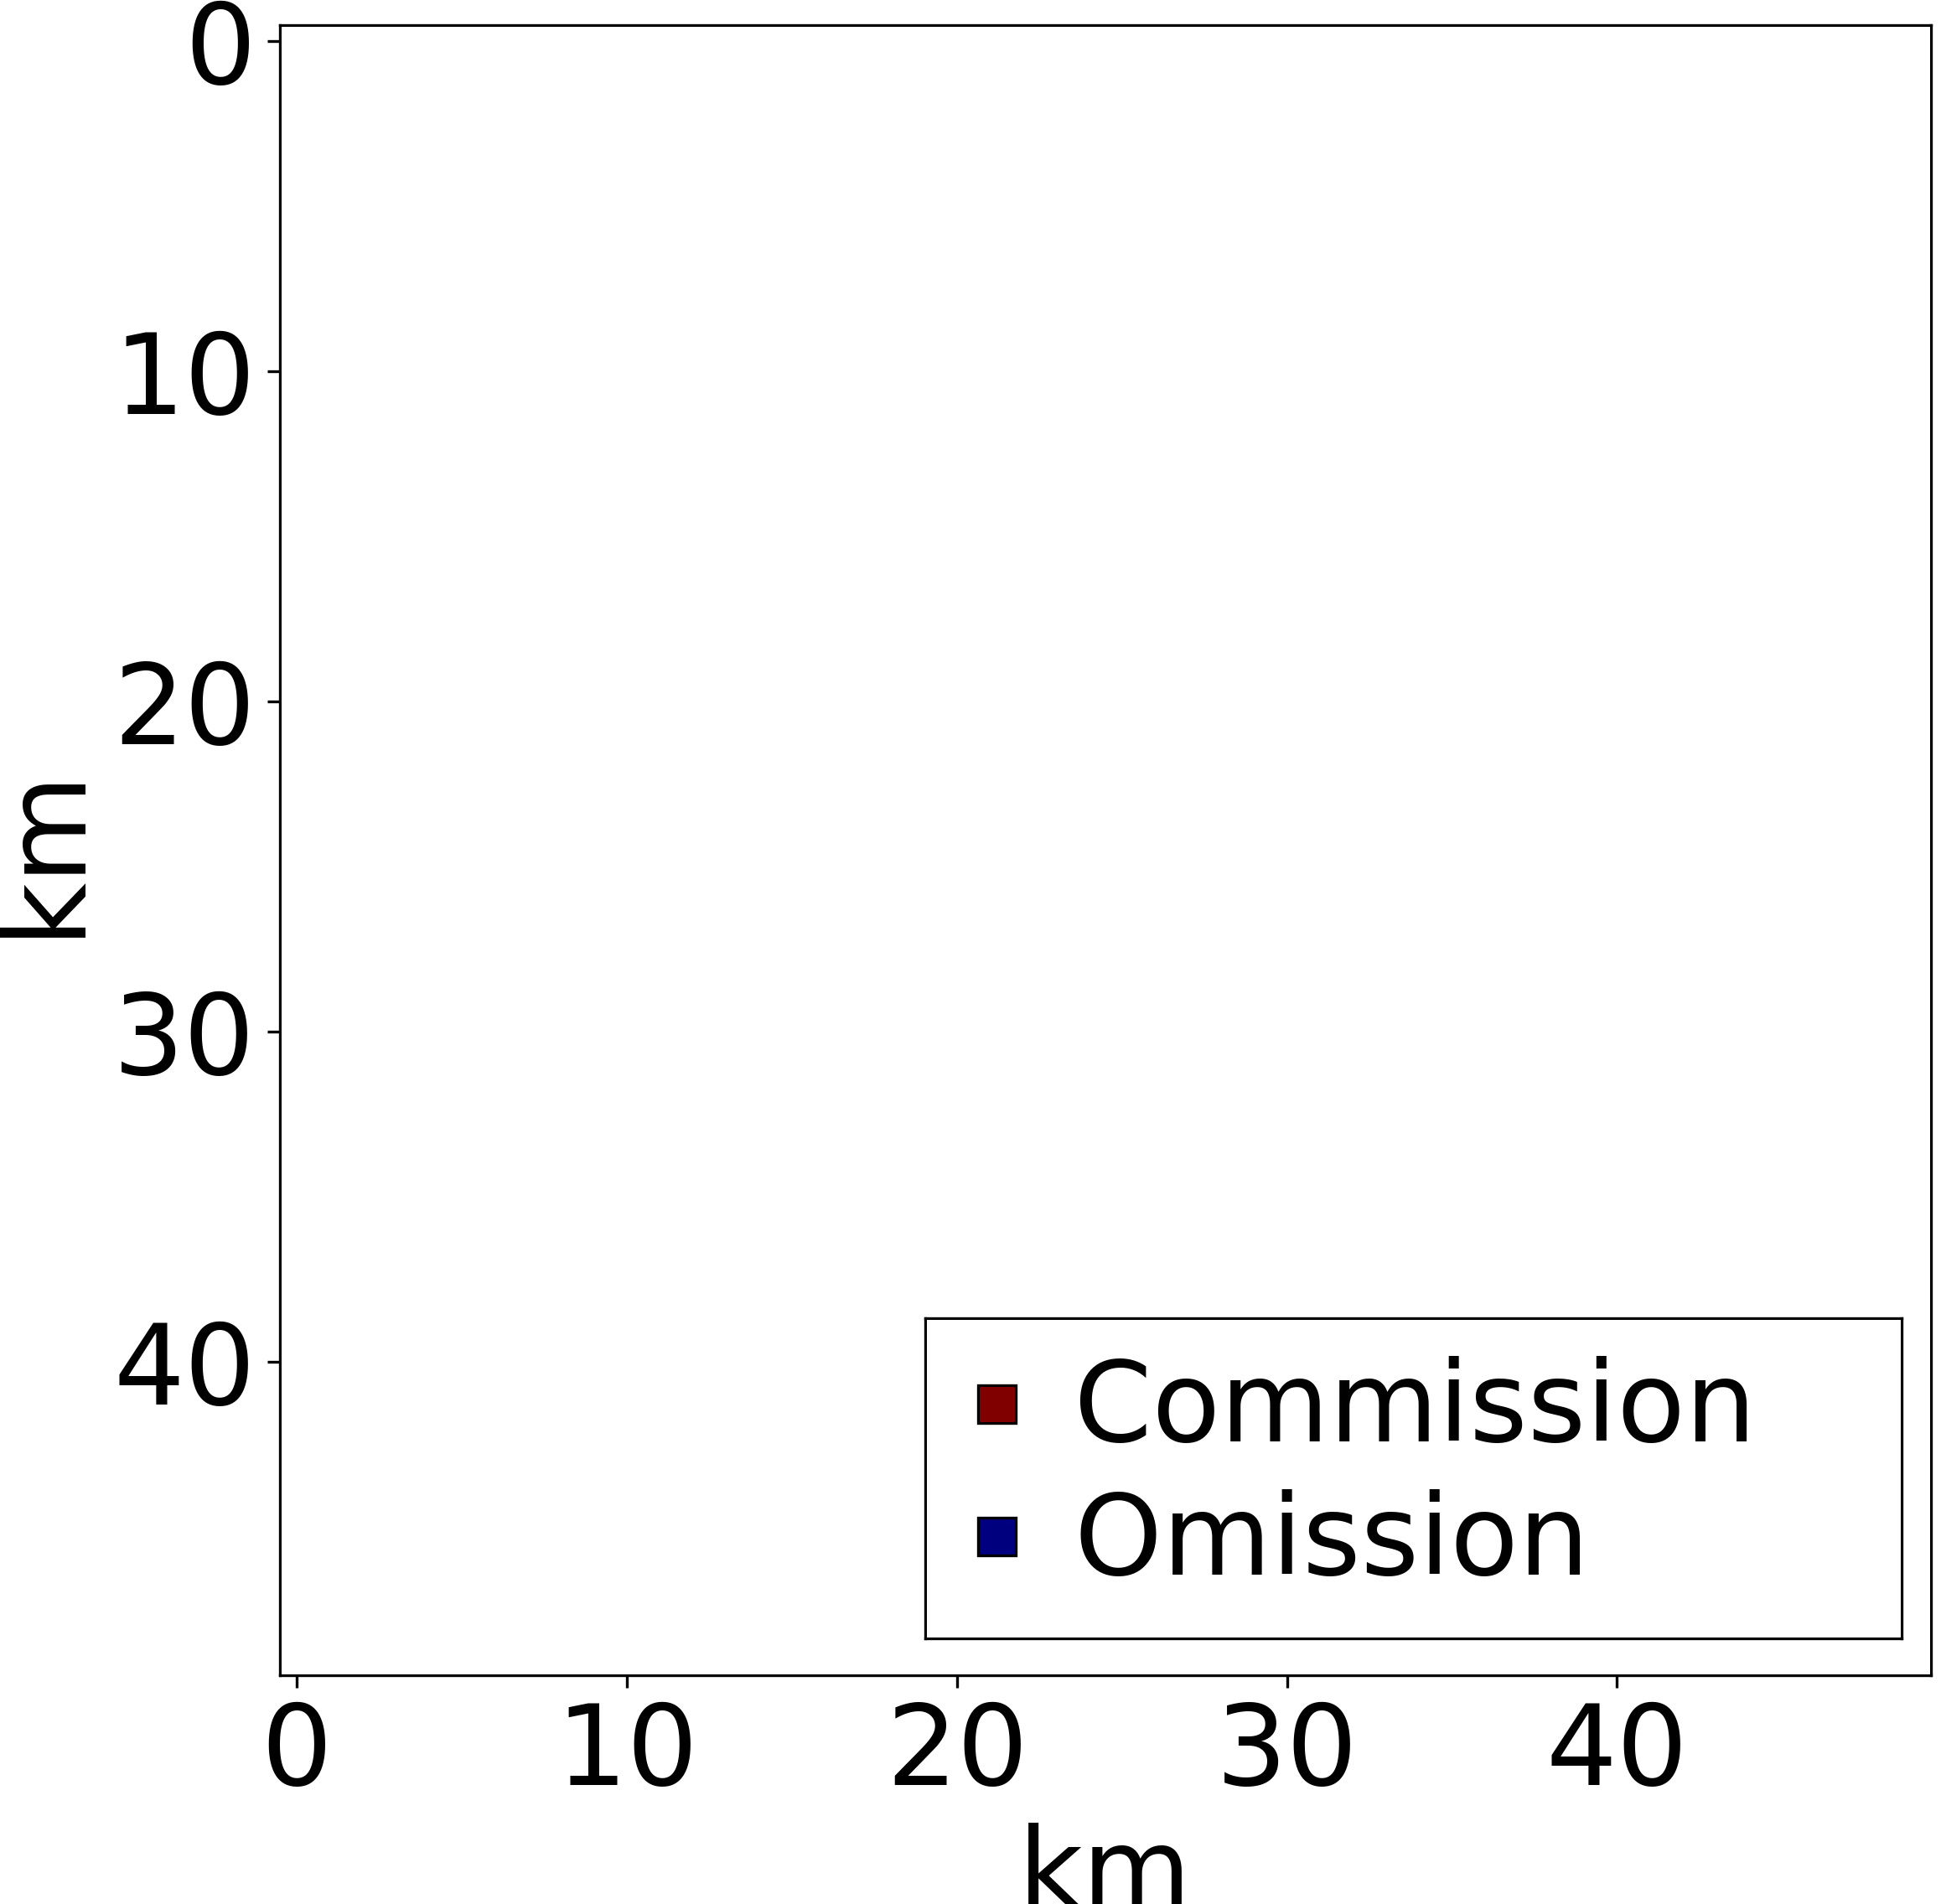
\includegraphics[height=0.25\textwidth]{exampleNetworkError3.png}
	\\
	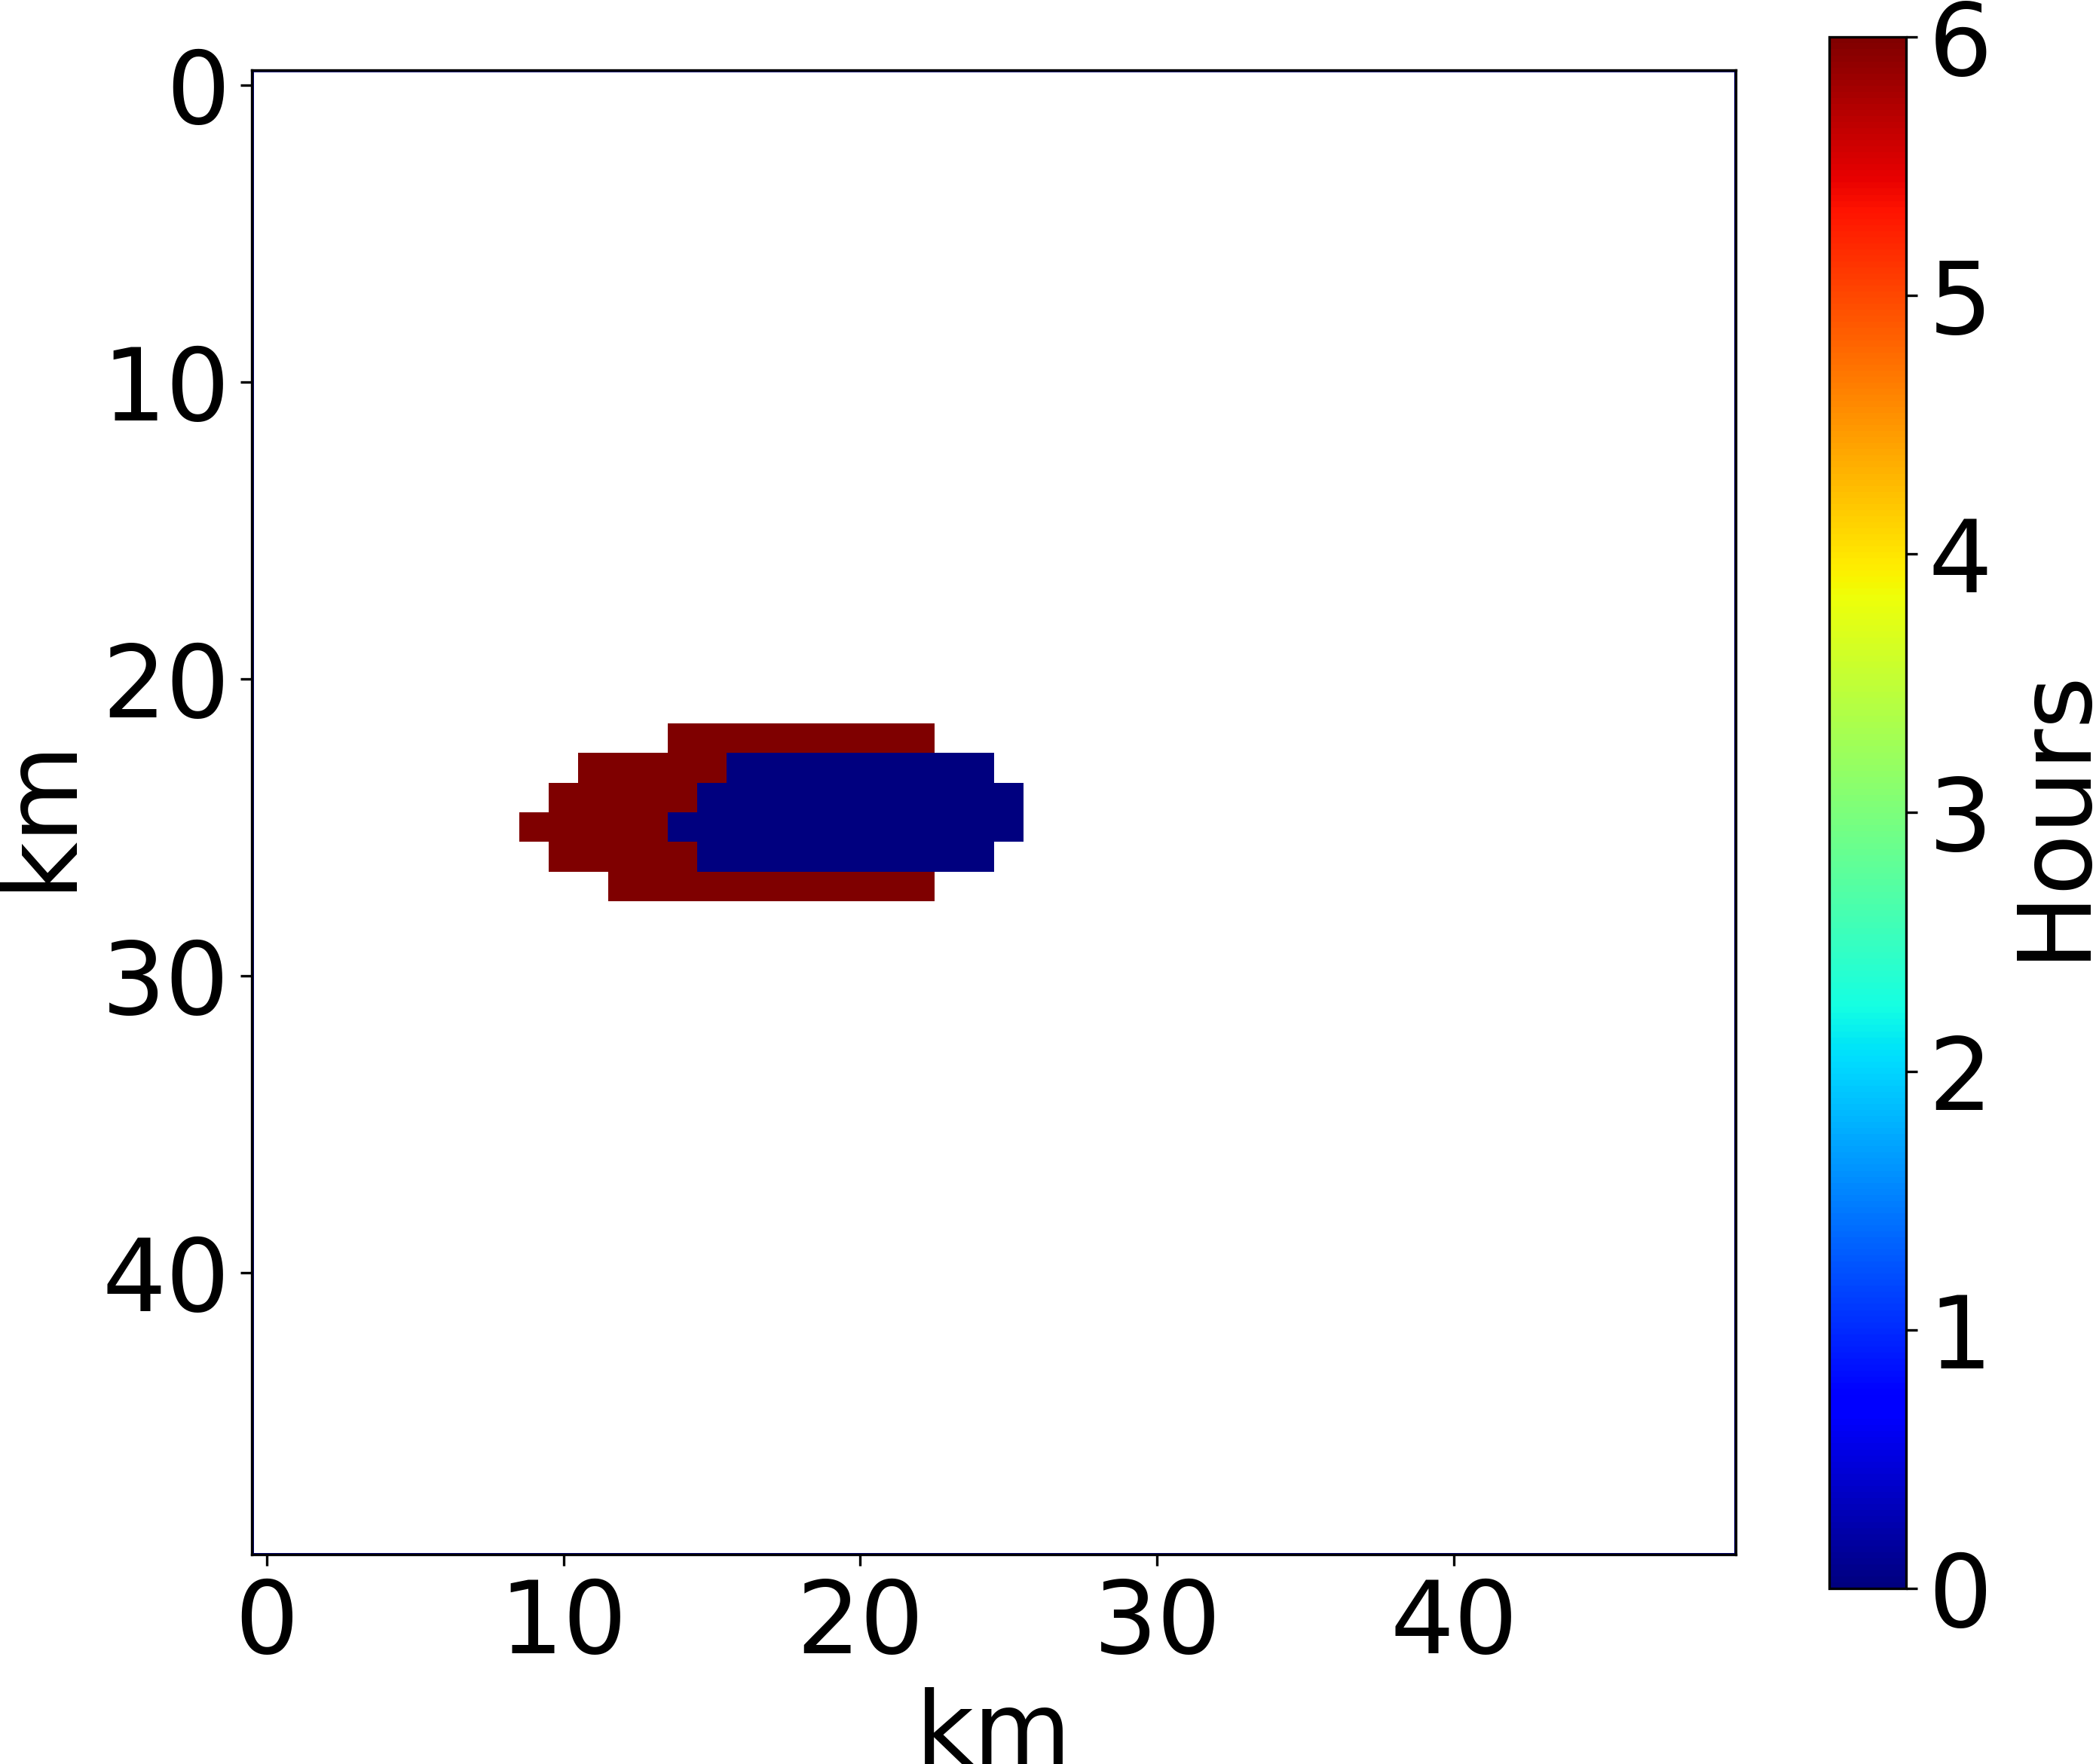
\includegraphics[height=0.25\textwidth]{exampleFusedFire4.png}
	~
	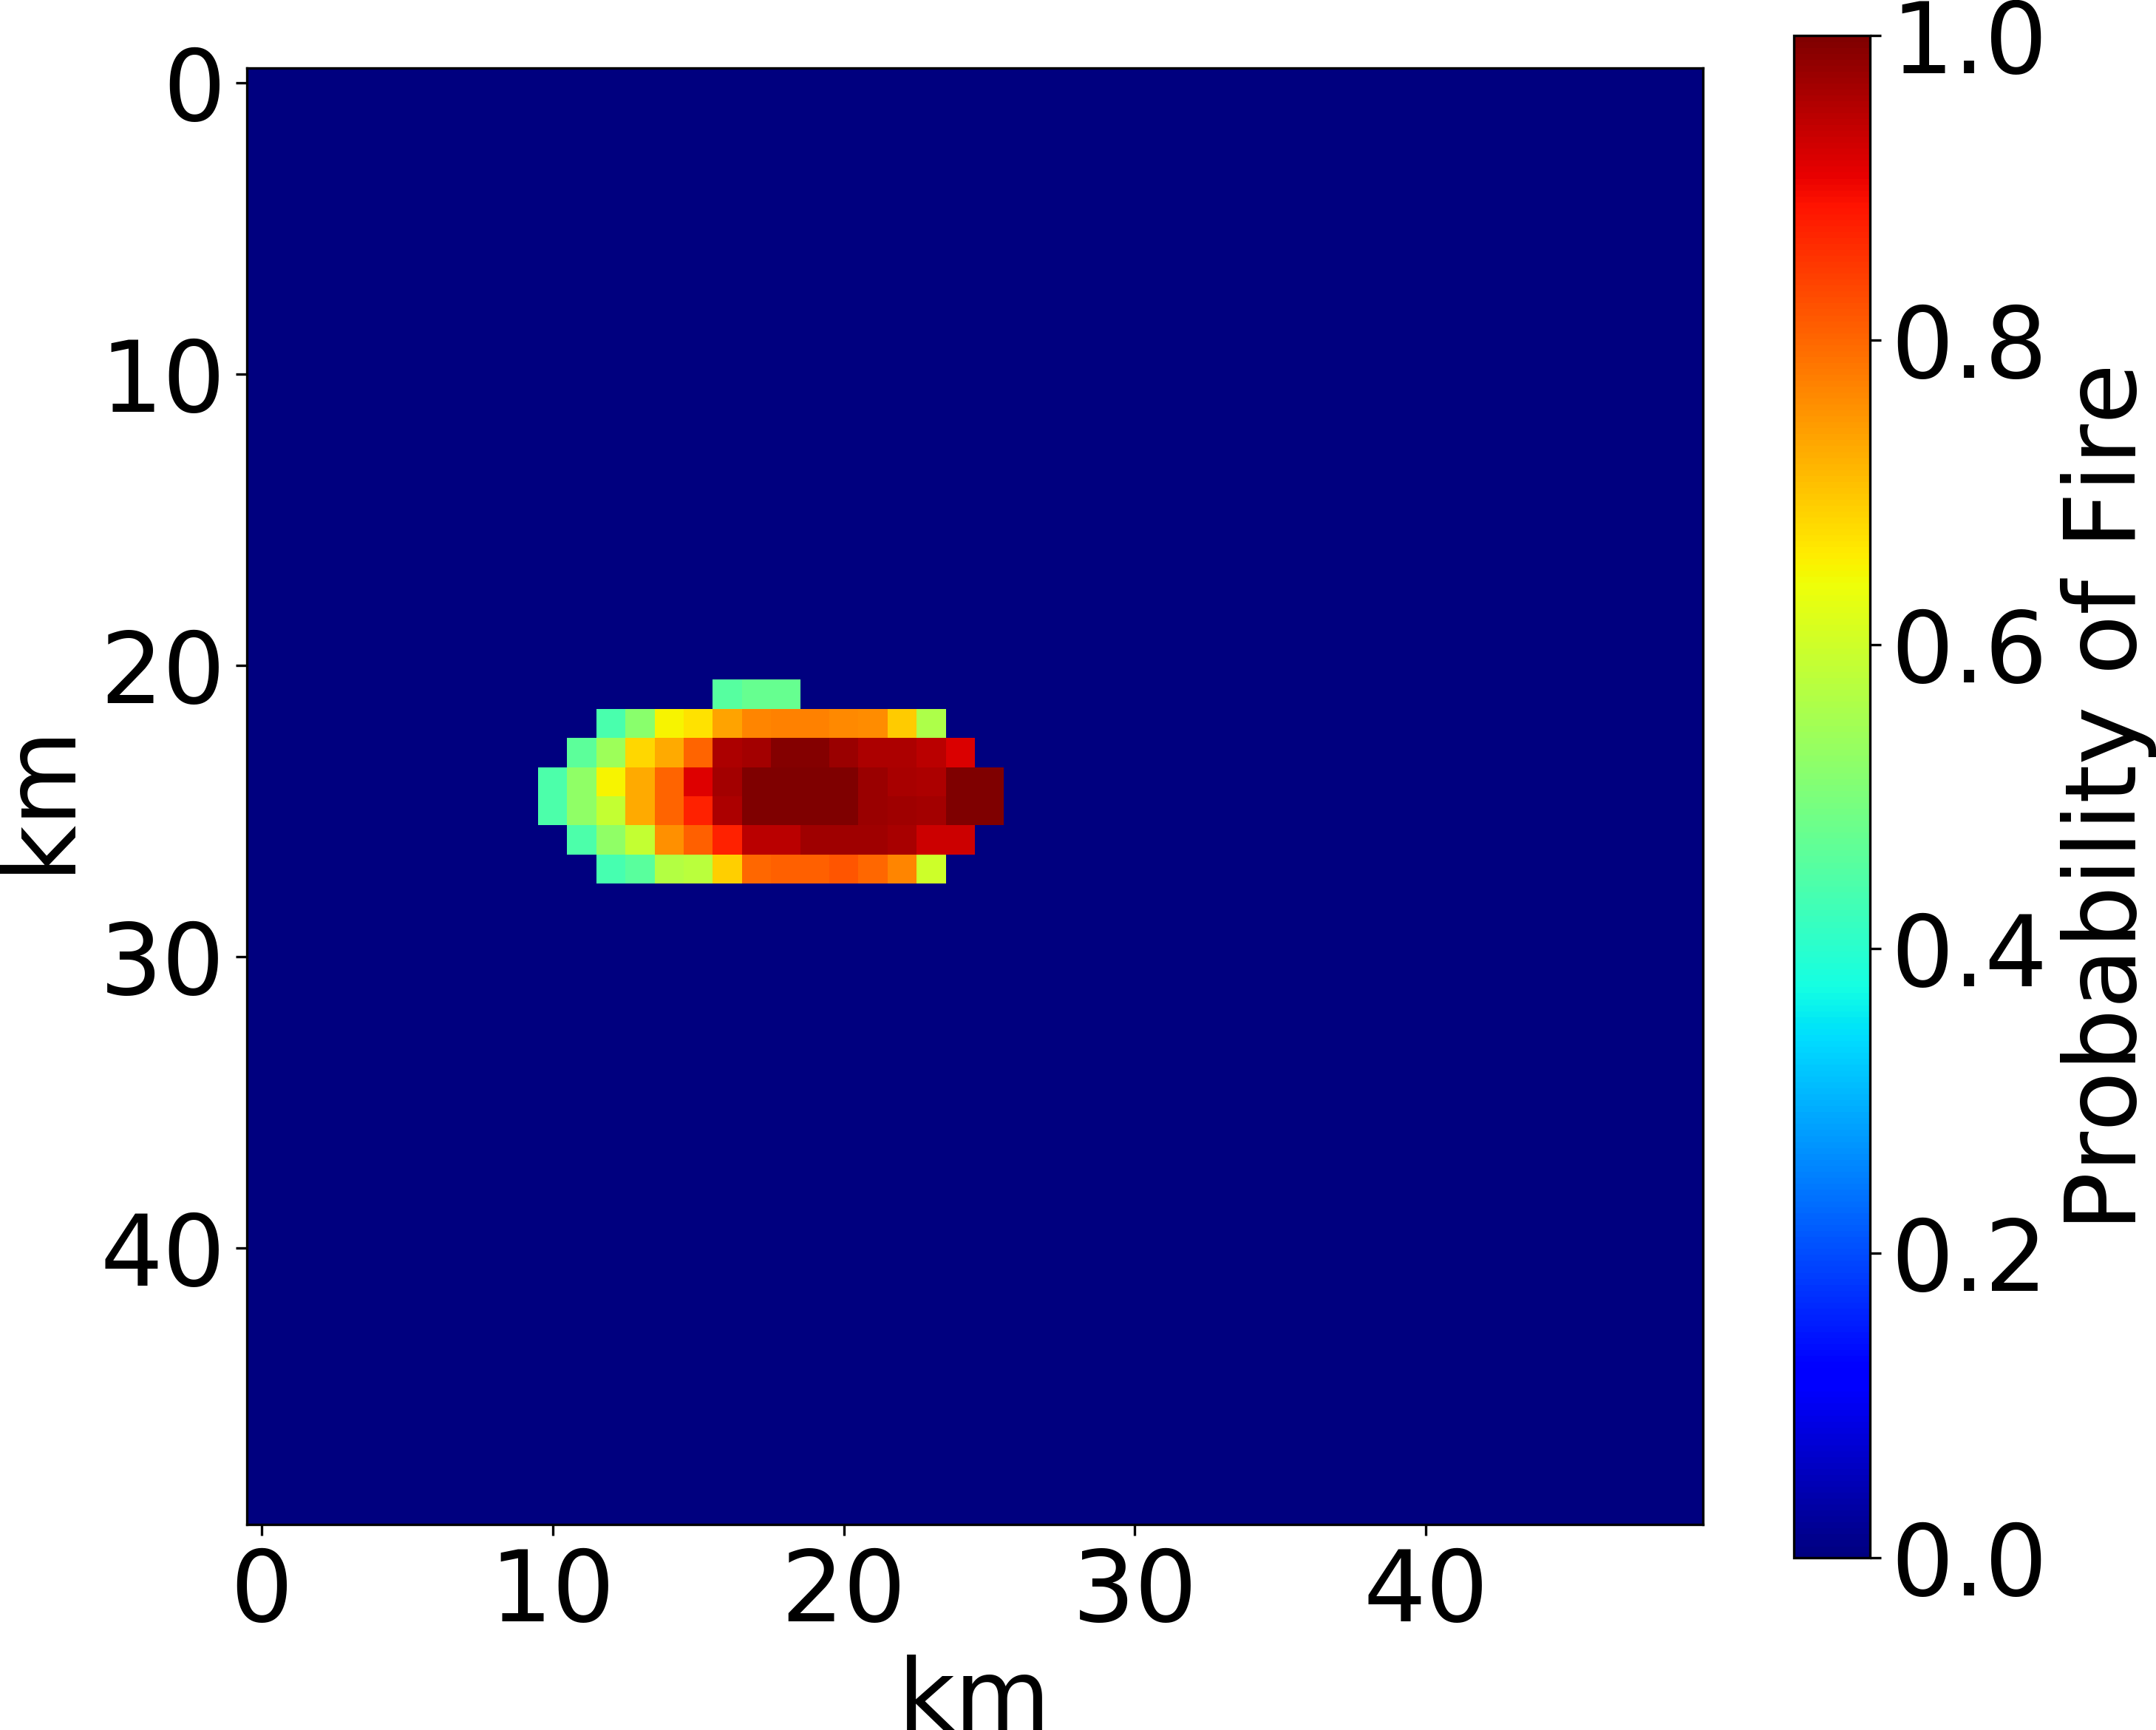
\includegraphics[height=0.25\textwidth]{exampleNetworkProcessed4.png}
	~
	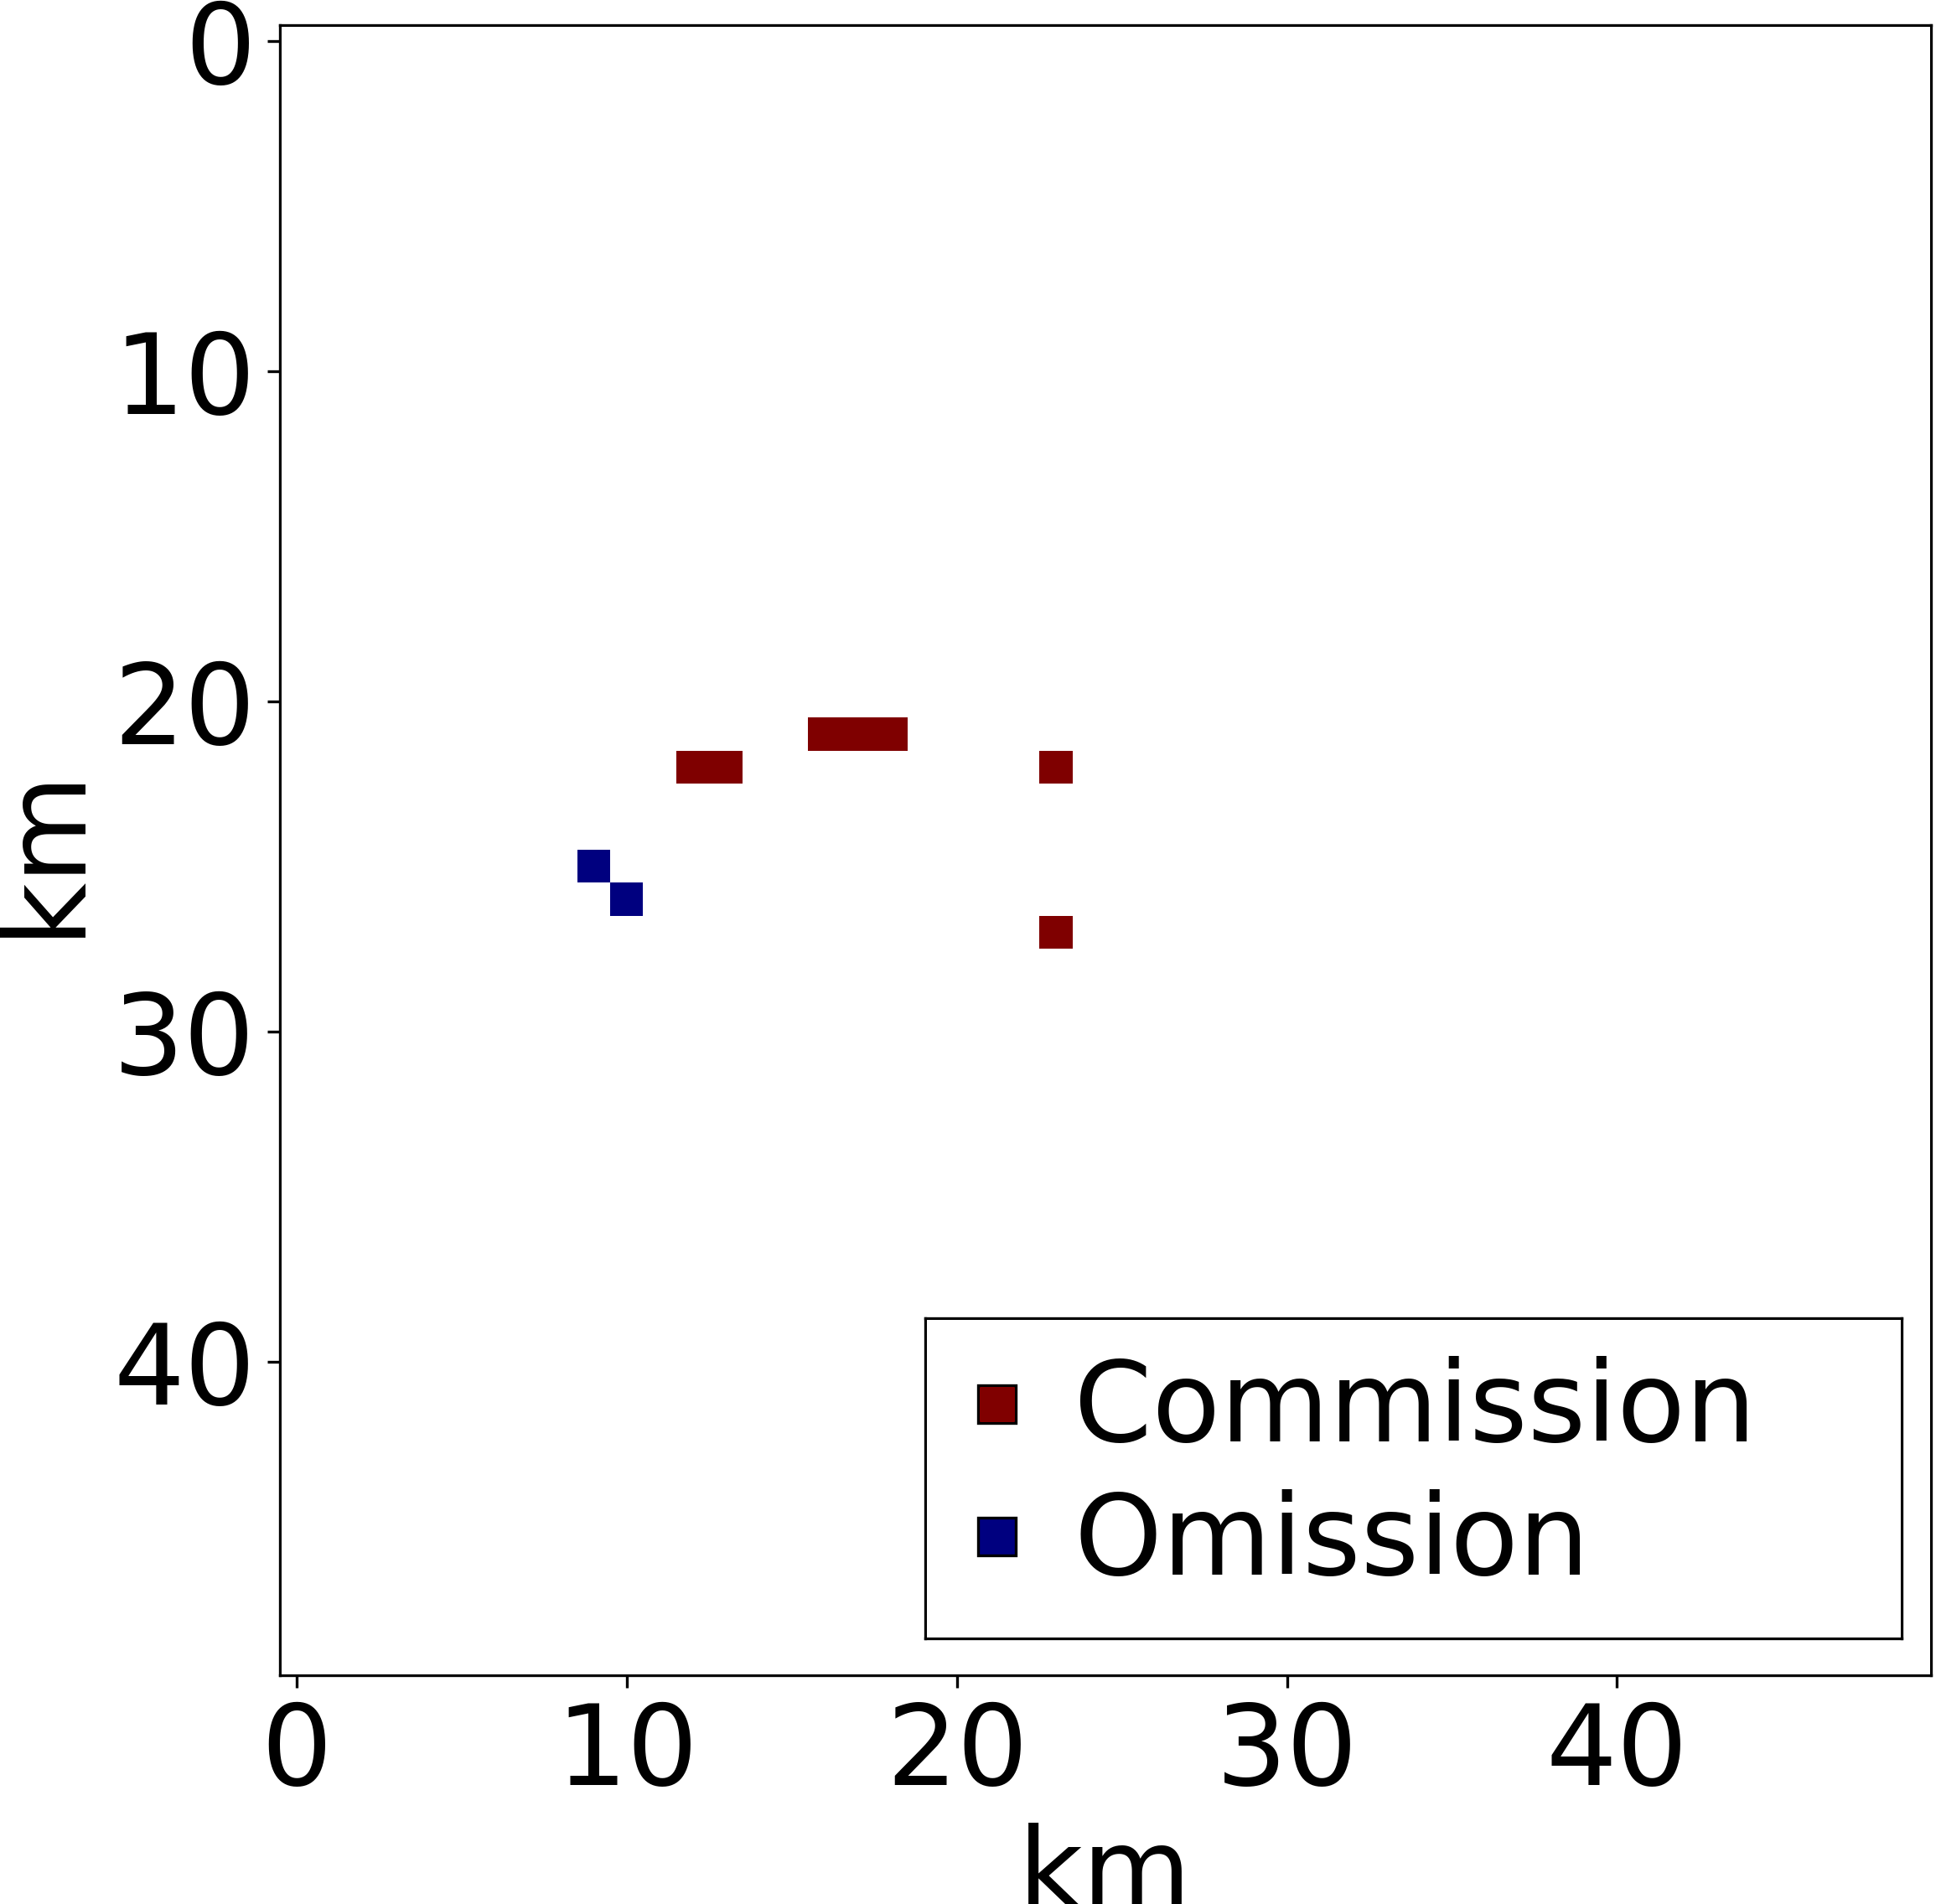
\includegraphics[height=0.25\textwidth]{exampleNetworkError4.png}
	\\
\hspace{0.035\textwidth}(a)\hspace{0.29\textwidth}(b)\hspace{0.31\textwidth}(c)
\caption{Example CNN prediction of fire perimeters (a) Simulation fire perimiter (blue) input to CNN (red) expected fire perimeter after 6 hours (b) CNN prediction of fire perimeter (c) Classification error }
\label{fig:exampleNetwork}       % Give a unique label
\end{figure*}


\section{Results}
\label{s:Results}

The robustness of the neural network to predict new fires was examined
by considering 3,000 test cases which were not included when training
the network (1,000 parameter sets with predictions 6 hours apart).
Sample CNN predictions from 5 of these test cases are
compared with simulation predictions in Fig.~\ref{fig:exampleNetwork}.
Figure~\ref{fig:exampleNetwork}a shows the initial and final fire perimeter
from the simulation.
Figure~\ref{fig:exampleNetwork}b shows the final fire perimeter predicted by the CNN.
Figure~\ref{fig:exampleNetwork}c highlights pixels which the CNN prediction did not match
the simulation predictions. Pixels shown as red represent commission
errors (false positive of fire), and pixels shown as blue represent omission errors
(false negative of fire).

The mean and 80, 90, and 95-Percentile (X\% of observations above)
precision, sensitivity, and F-measure of the 3,000 test
cases are shown in Table~\ref{tab:metrics}.
\begin{table}[htb]
\centering
% table caption is above the table
\caption{Performance Metrics of CNN Predictions of Test Cases}
\label{tab:metrics}       % Give a unique label
% For LaTeX tables use
\begin{tabular*}{0.45\textwidth}{l @{\extracolsep{\fill}} cccc}
\hline\noalign{\smallskip}
Parameter & Mean & 80\% & 90\% & 95\%\\
\noalign{\smallskip}\hline\noalign{\smallskip}
Precision & 0.97 & 0.95 & 0.85 & 0.79\\
Sensitivity & 0.92 & 0.80 & 0.67 & 0.59\\
F-Measure & 0.93 & 0.86 & 0.80 & 0.73\\
\noalign{\smallskip}\hline
\end{tabular*}
\end{table}
The distribution of F-measure for the 3,000 test cases are shown
in Fig.~\ref{fig:fMeasureDistribution}.




\begin{figure}[htbp]
\centering
% Use the relevant command to insert your figure file.
% For example, with the graphicx package use
  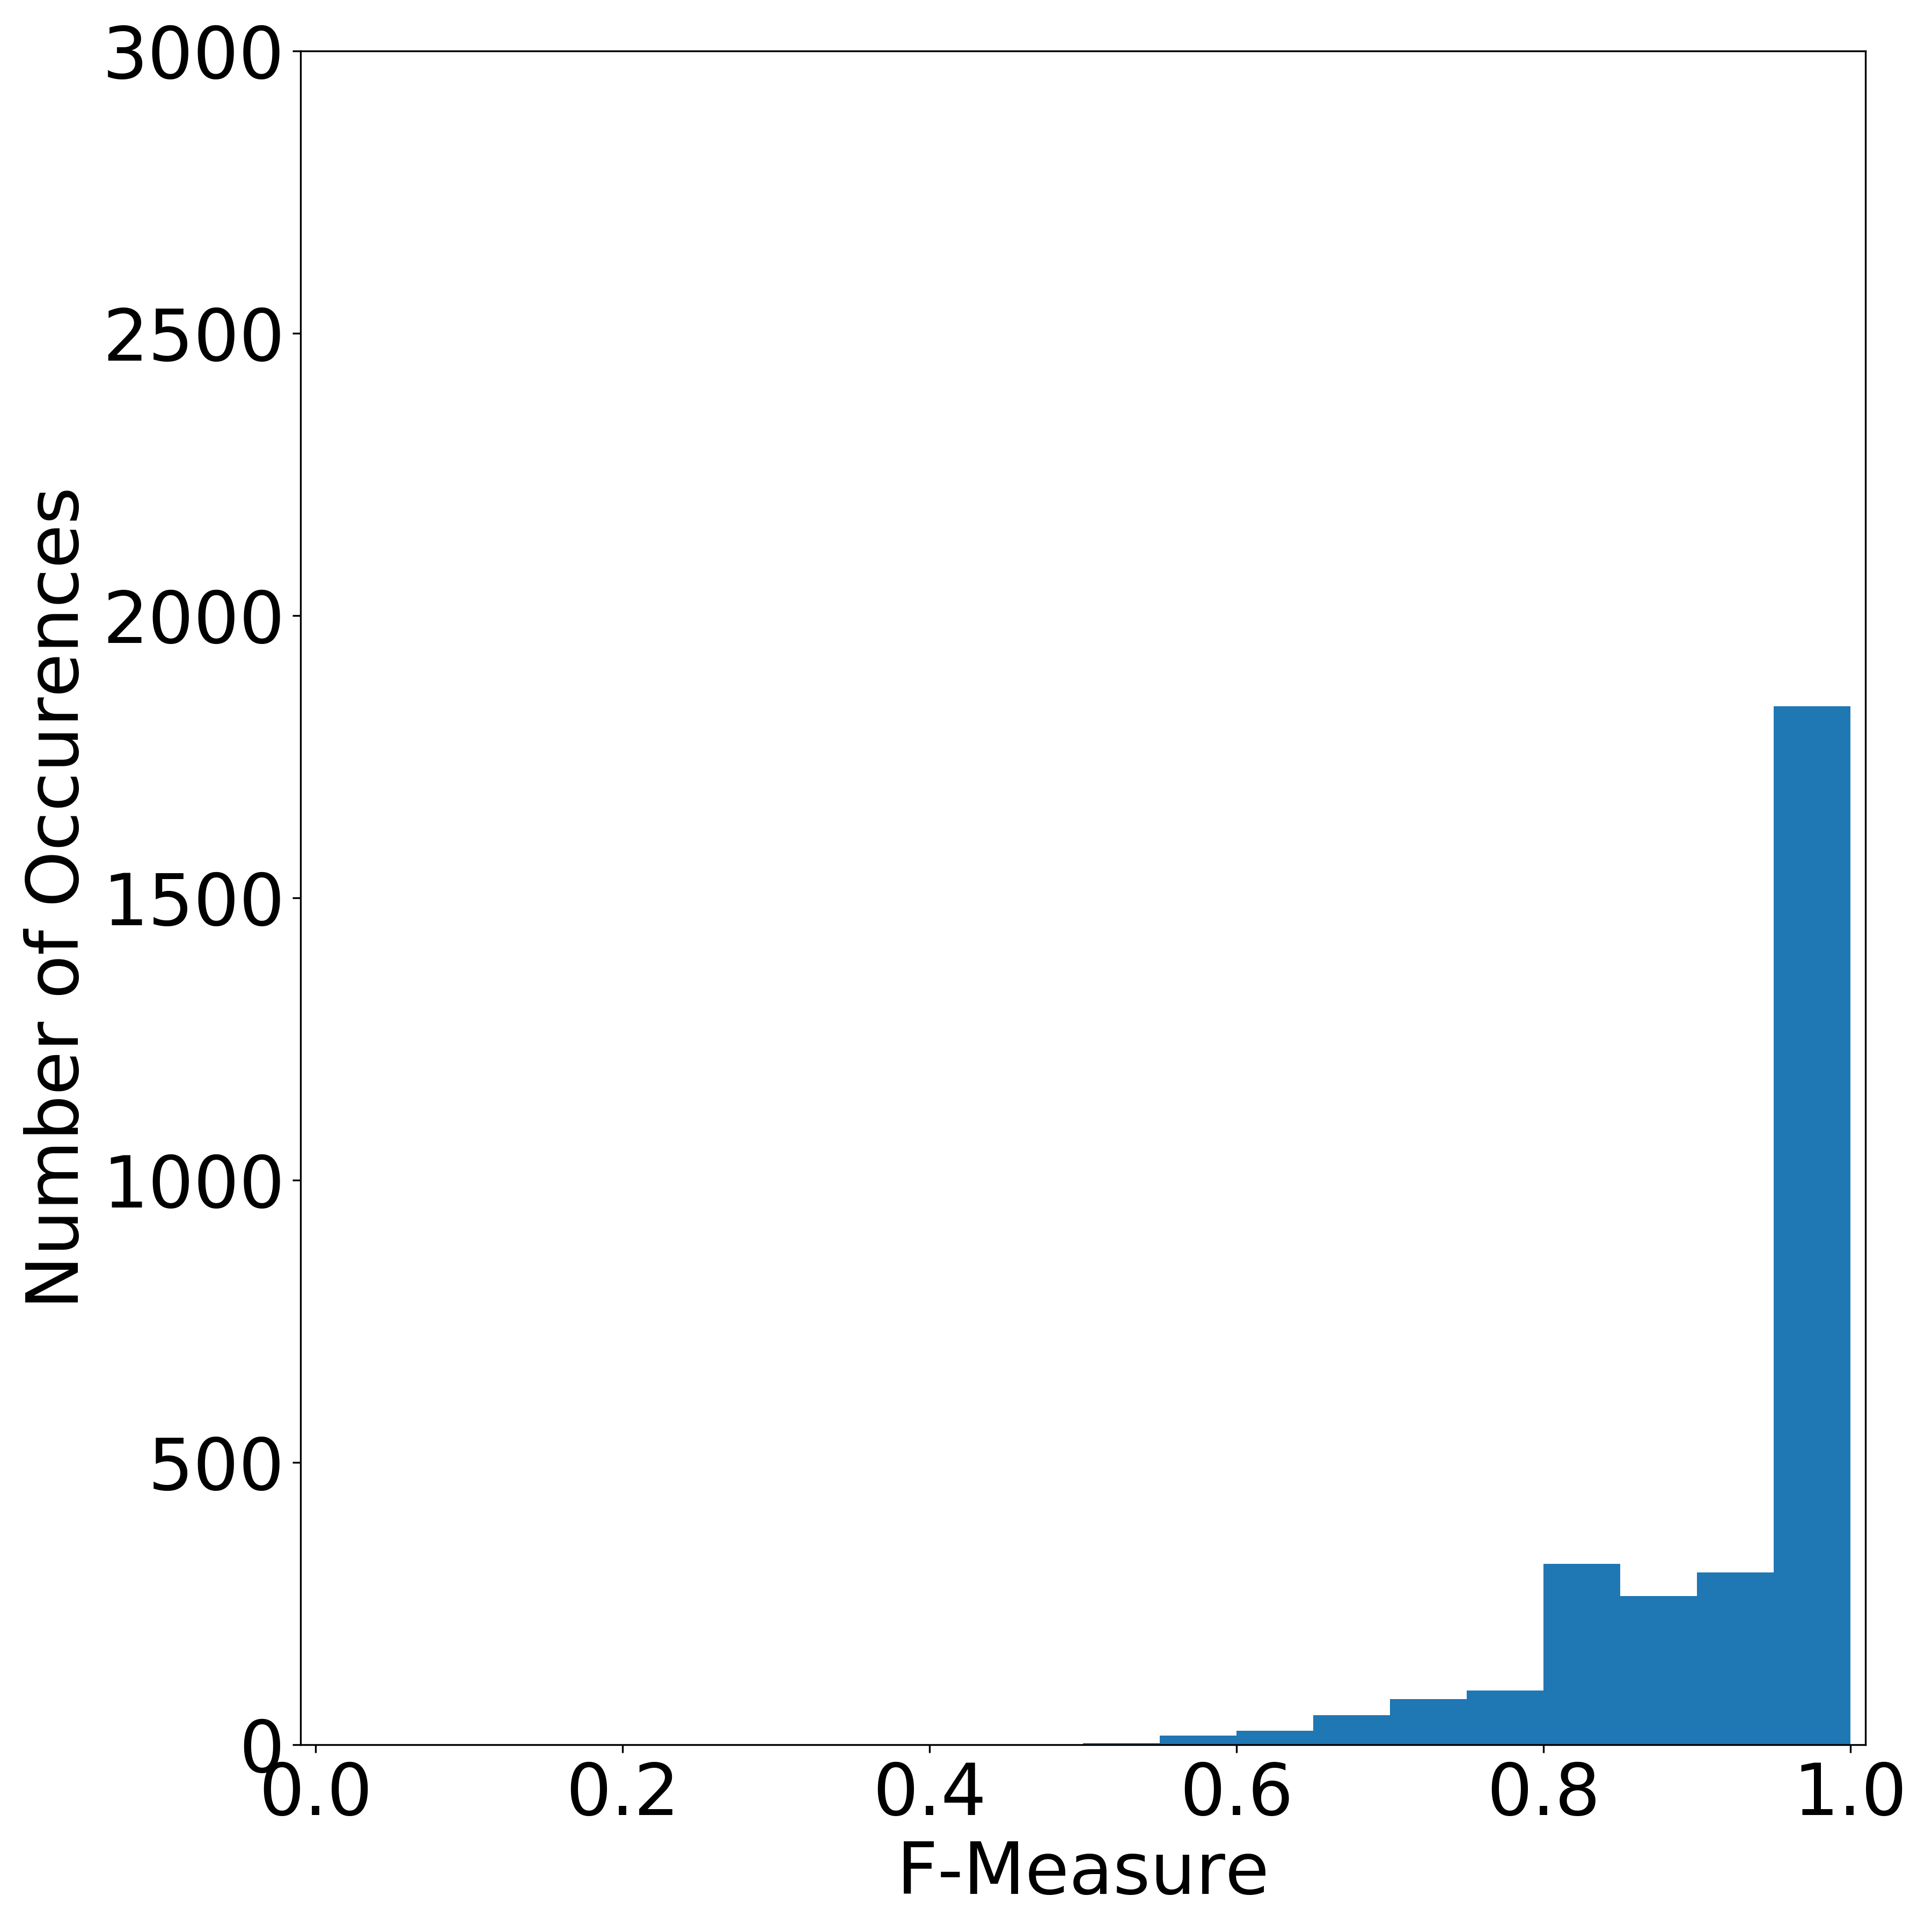
\includegraphics[width=0.45\textwidth]{rothermelFull_cnnModel3_F_pdf.png}
% figure caption is below the figure
\caption{F-Measure distribution of CNN Predictions of Test Cases.}
\label{fig:fMeasureDistribution}       % Give a unique label
\end{figure}



















\section{Discussion}
\label{s:Discussion}

The overall shape of the fire perimeter predicted by the CNN is aligned
with the simulations for the 3,000 test cases examined in this work.
The fire perimeters predicted by the CNN do not contain non-physical
holes or spotting. The direction of maximum growth is captured well.
Figure~\ref{fig:fMeasureDistribution} shows a sharp drop in number of
occurrences at $F < 0.8$. Examining the cases where $F < 0.8$, it
was found 82\% had an initial fire size of 9 pixels or less, as
shown in Fig.~\ref{fig:fireSize}. Since a CNN relies on feature
recognition, low feature density in the inputs leads to a decrease in
the accuracy of the model.

\begin{figure}[tbp]
\centering
% Use the relevant command to insert your figure file.
% For example, with the graphicx package use
  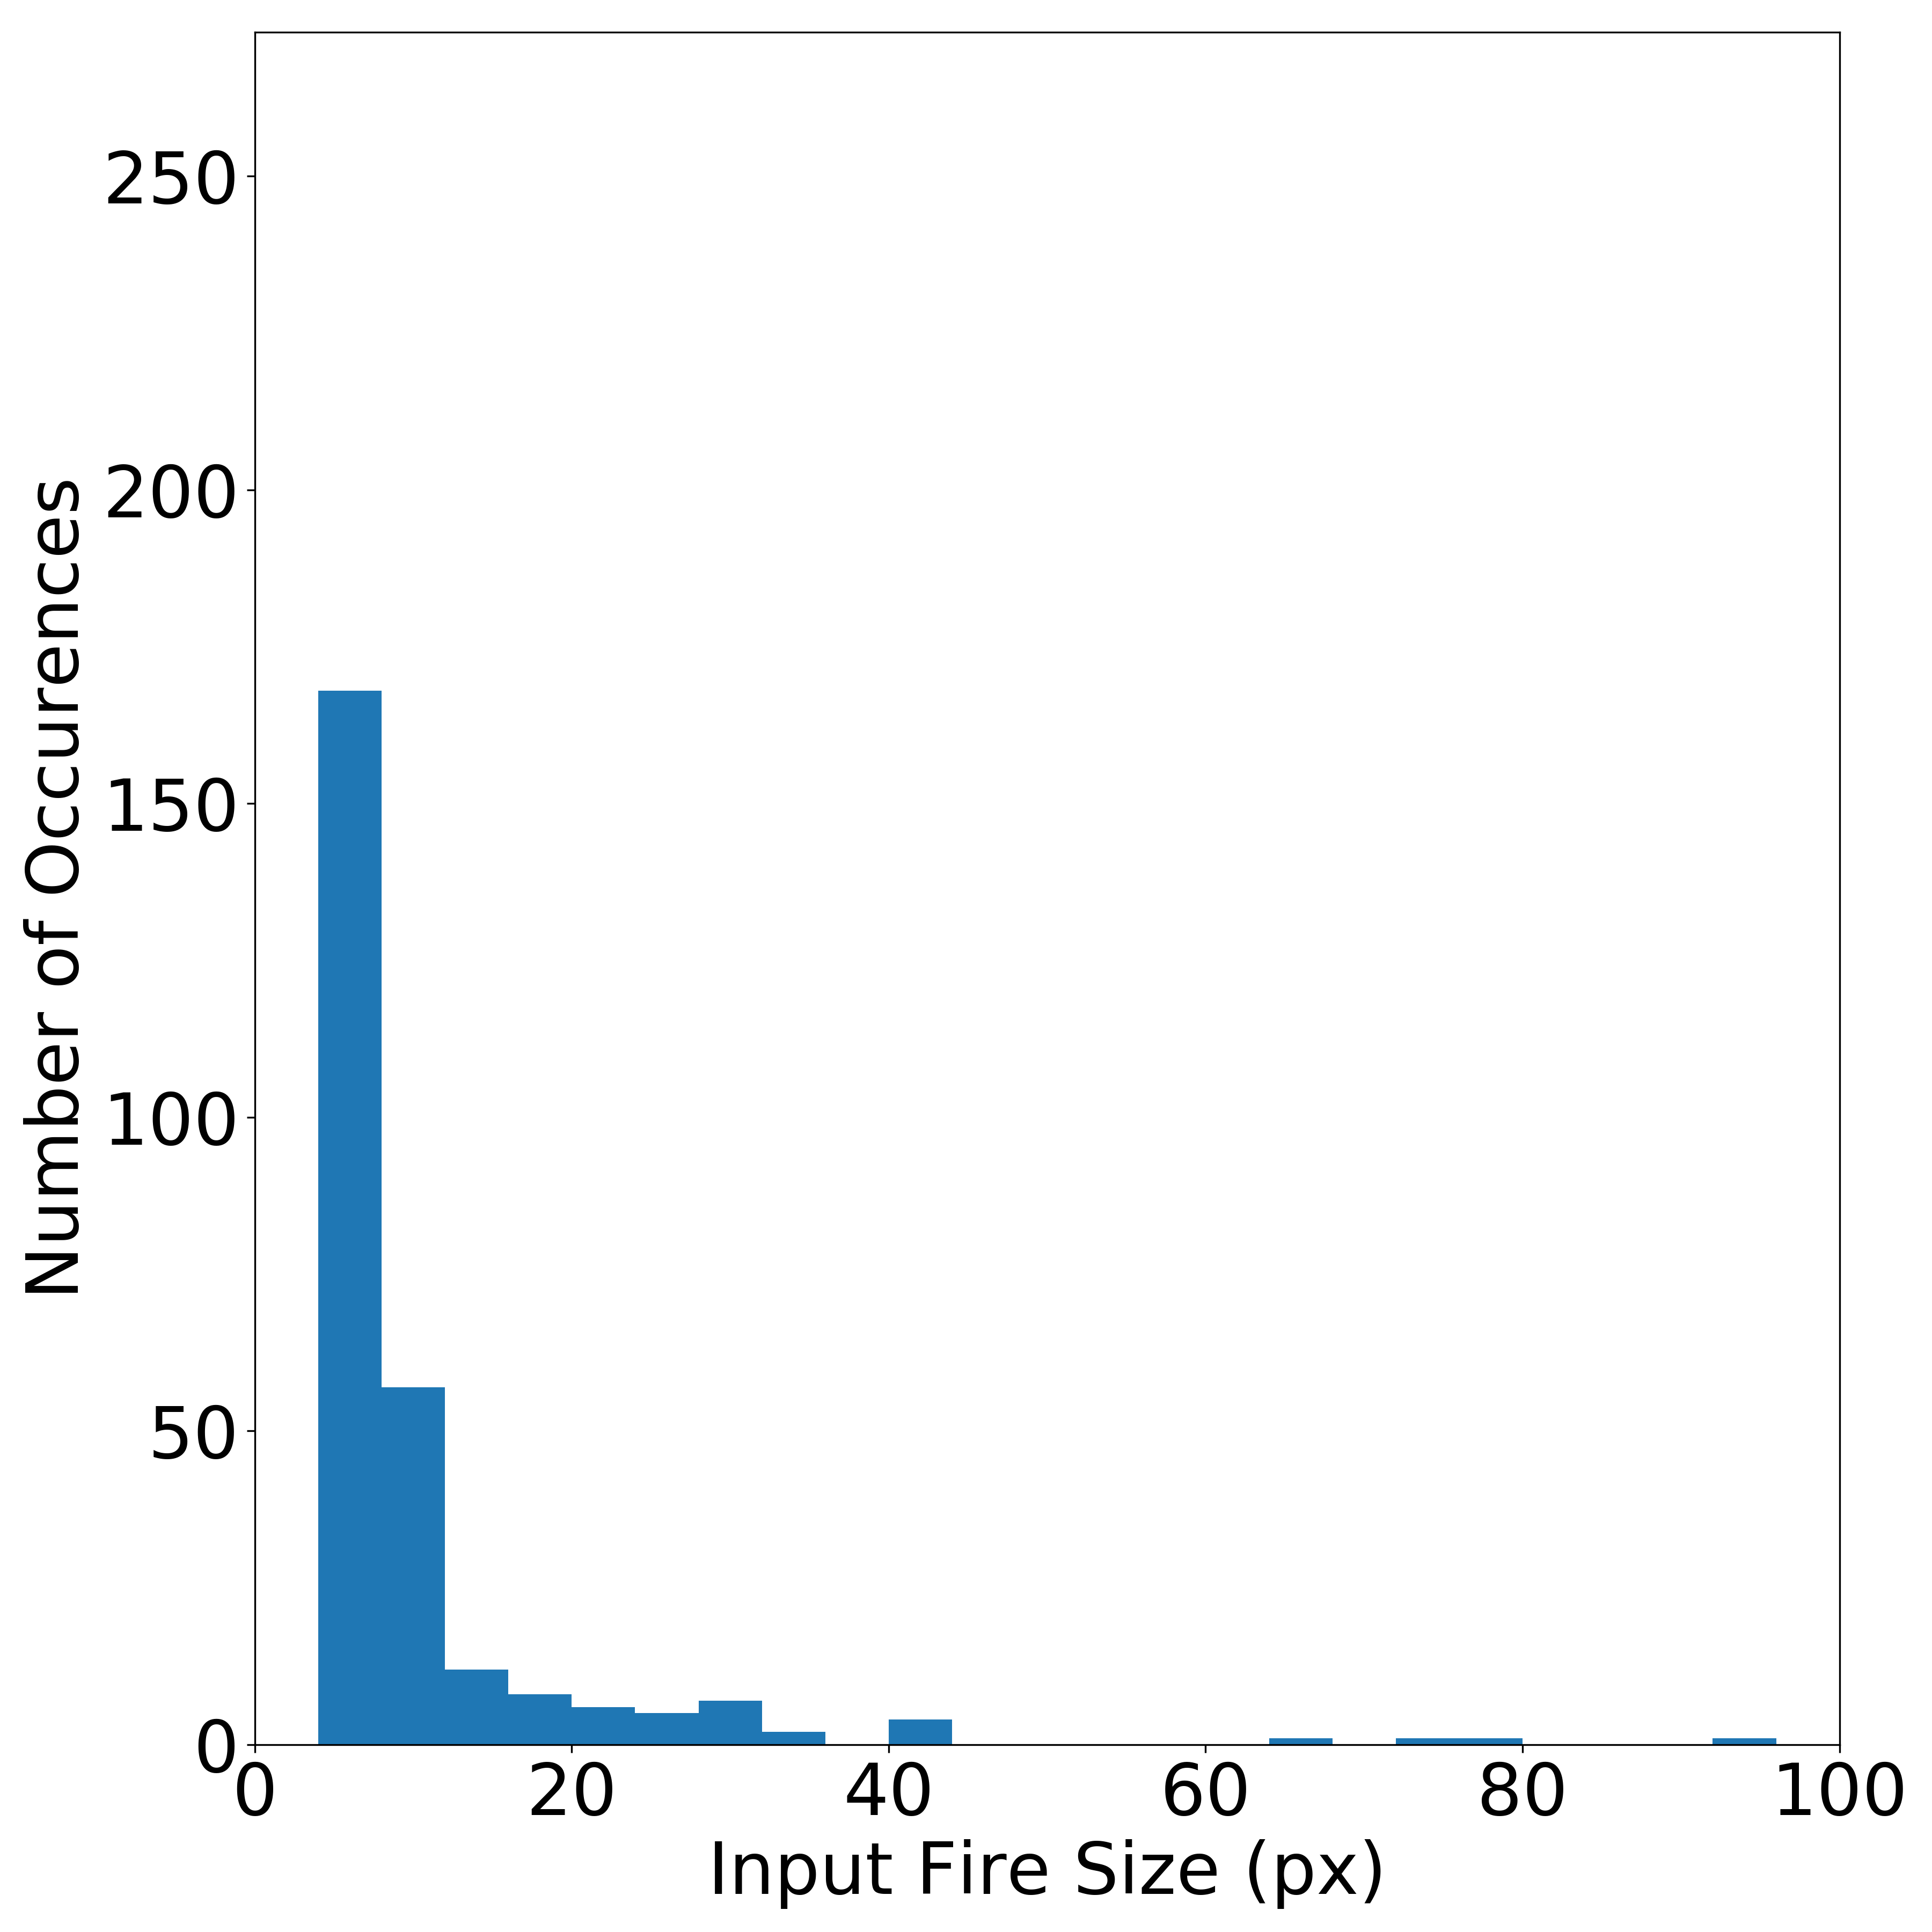
\includegraphics[width=0.45\textwidth]{rothermelFull_cnnModel3_fireSize_when_F_lt_080.png}
% figure caption is below the figure
\caption{Distribution of final fire size for all cases where $F < 0.8$.}
\label{fig:fireSize}       % Give a unique label
\end{figure}

\begin{figure}[tbp]
\centering
% Use the relevant command to insert your figure file.
% For example, with the graphicx package use
  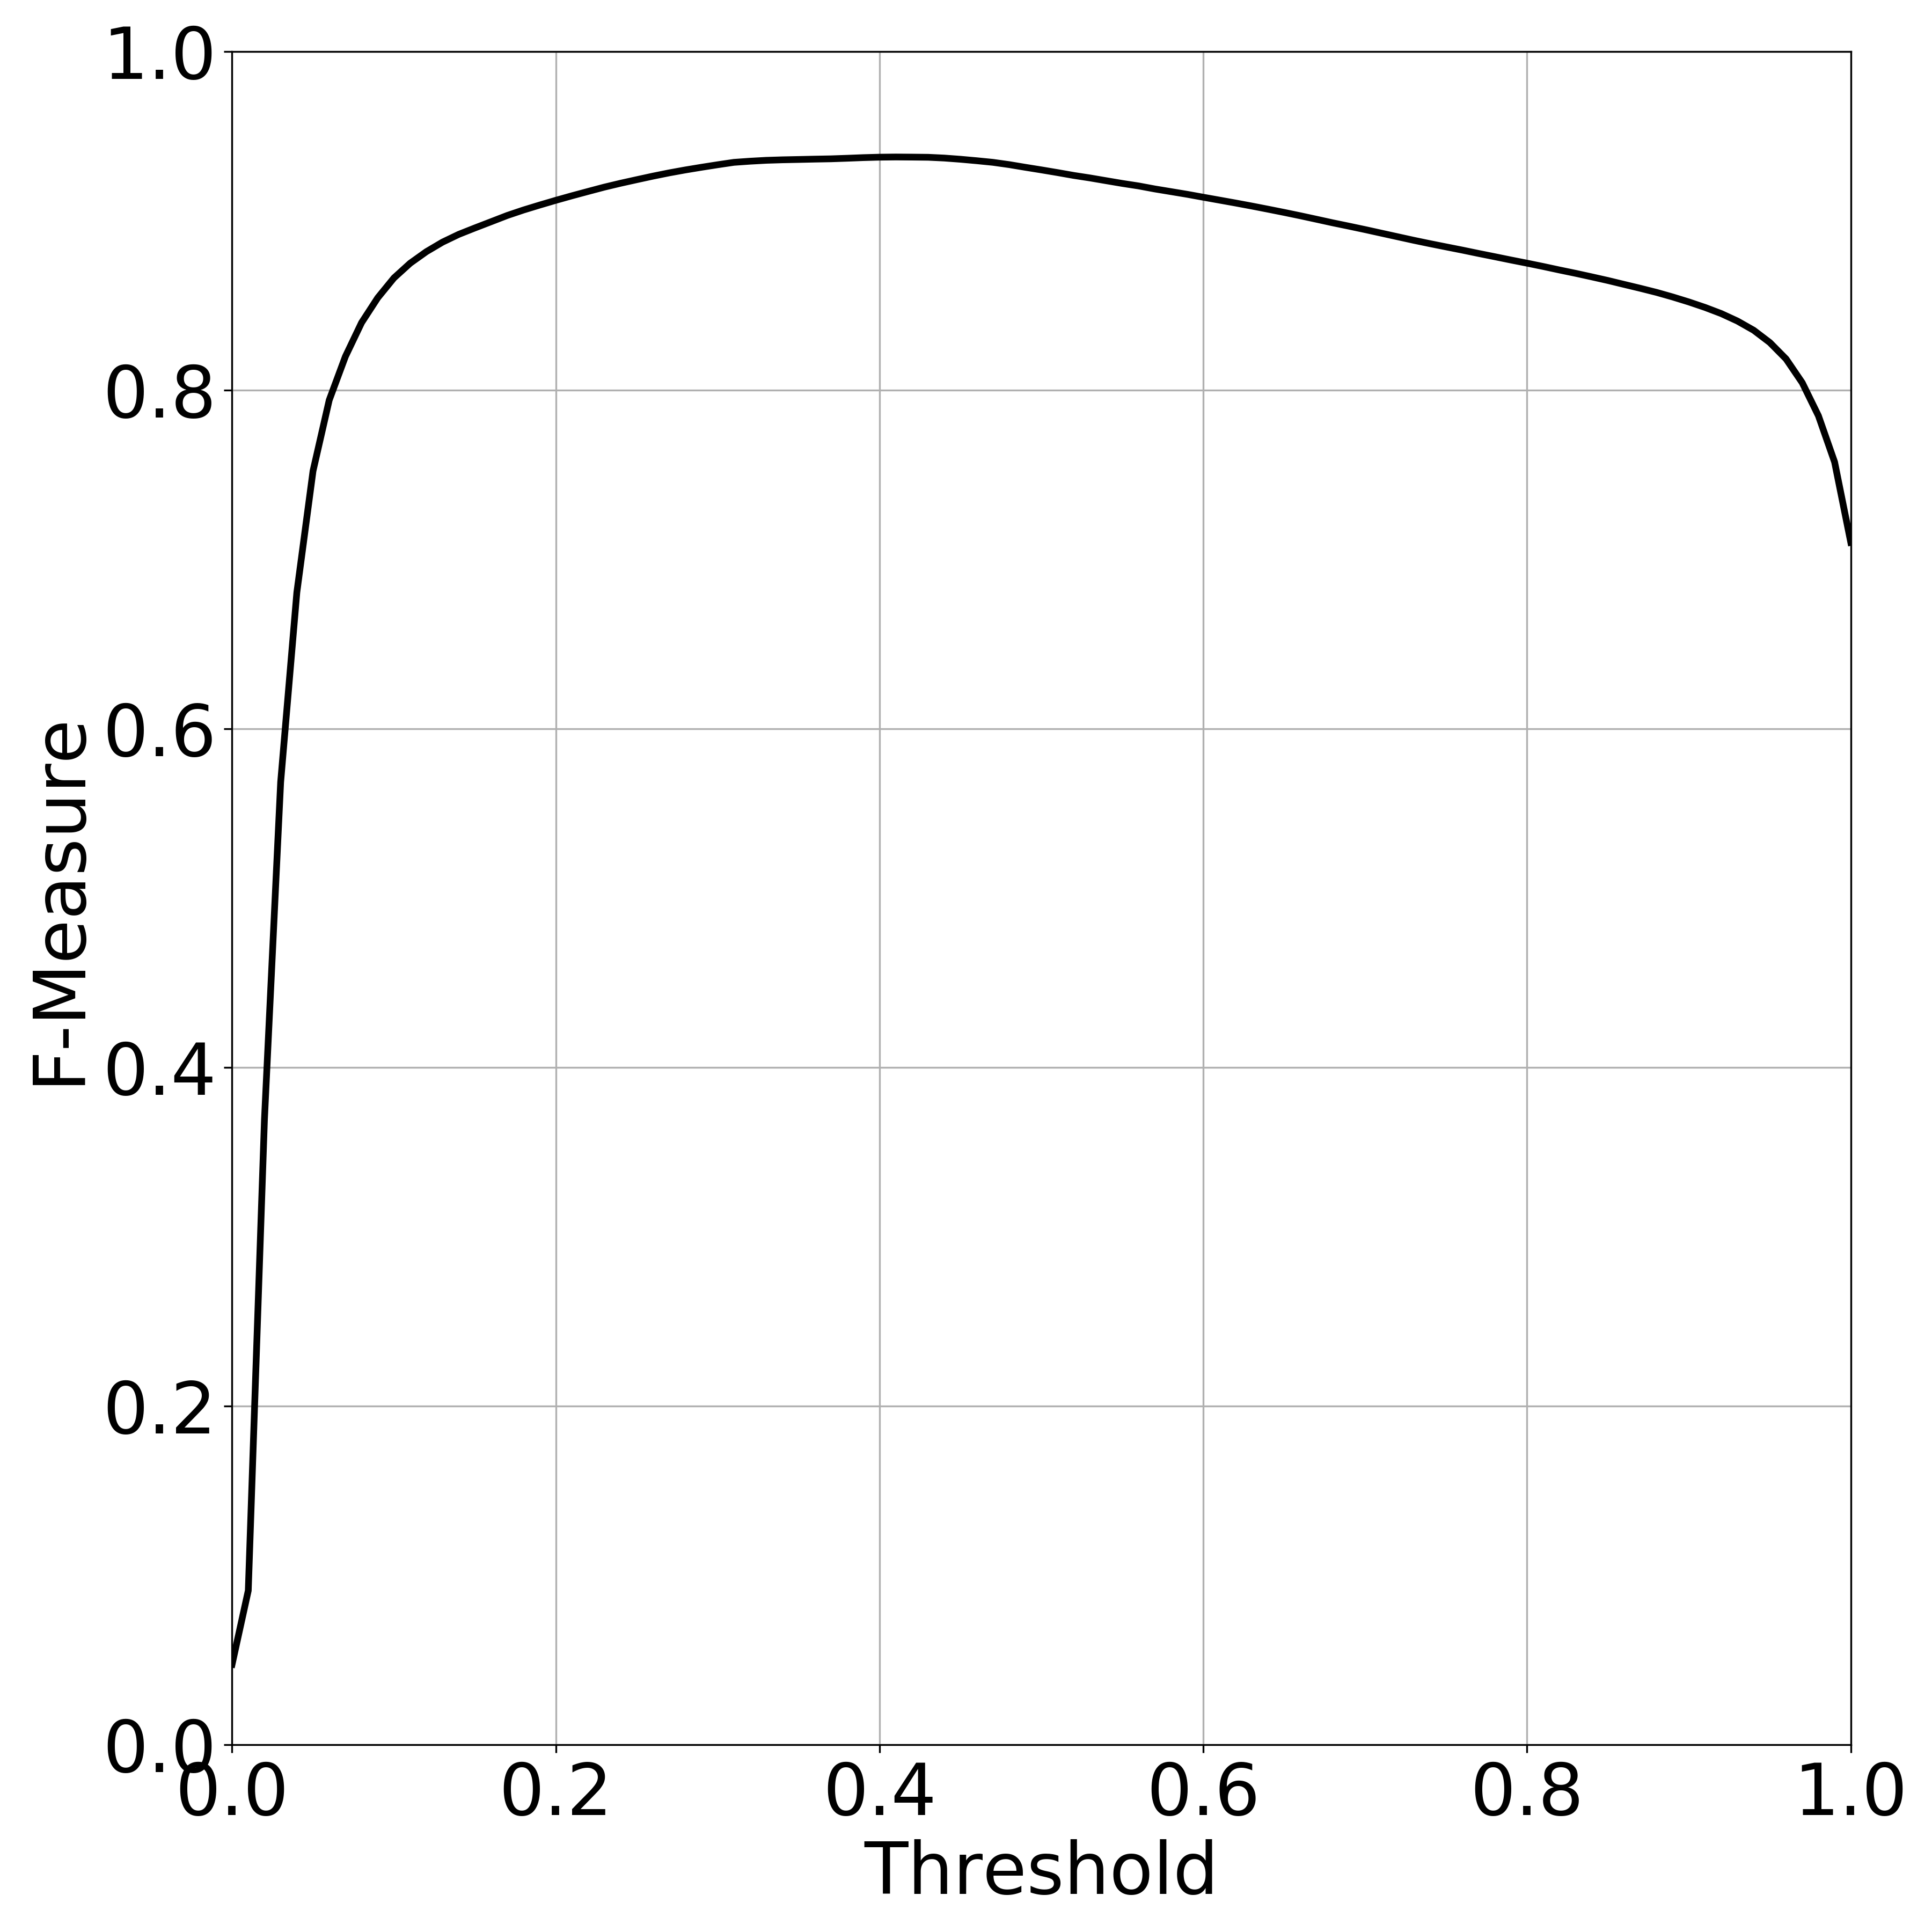
\includegraphics[width=0.45\textwidth]{optimalThreshold.png}
% figure caption is below the figure
\caption{Mean F-Measure of CNN predictions of 27,000 training data for different threshold values.}
\label{fig:fMeasureVsThreshold}       % Give a unique label
\end{figure}



\begin{figure*}[htbp]
  \centering
	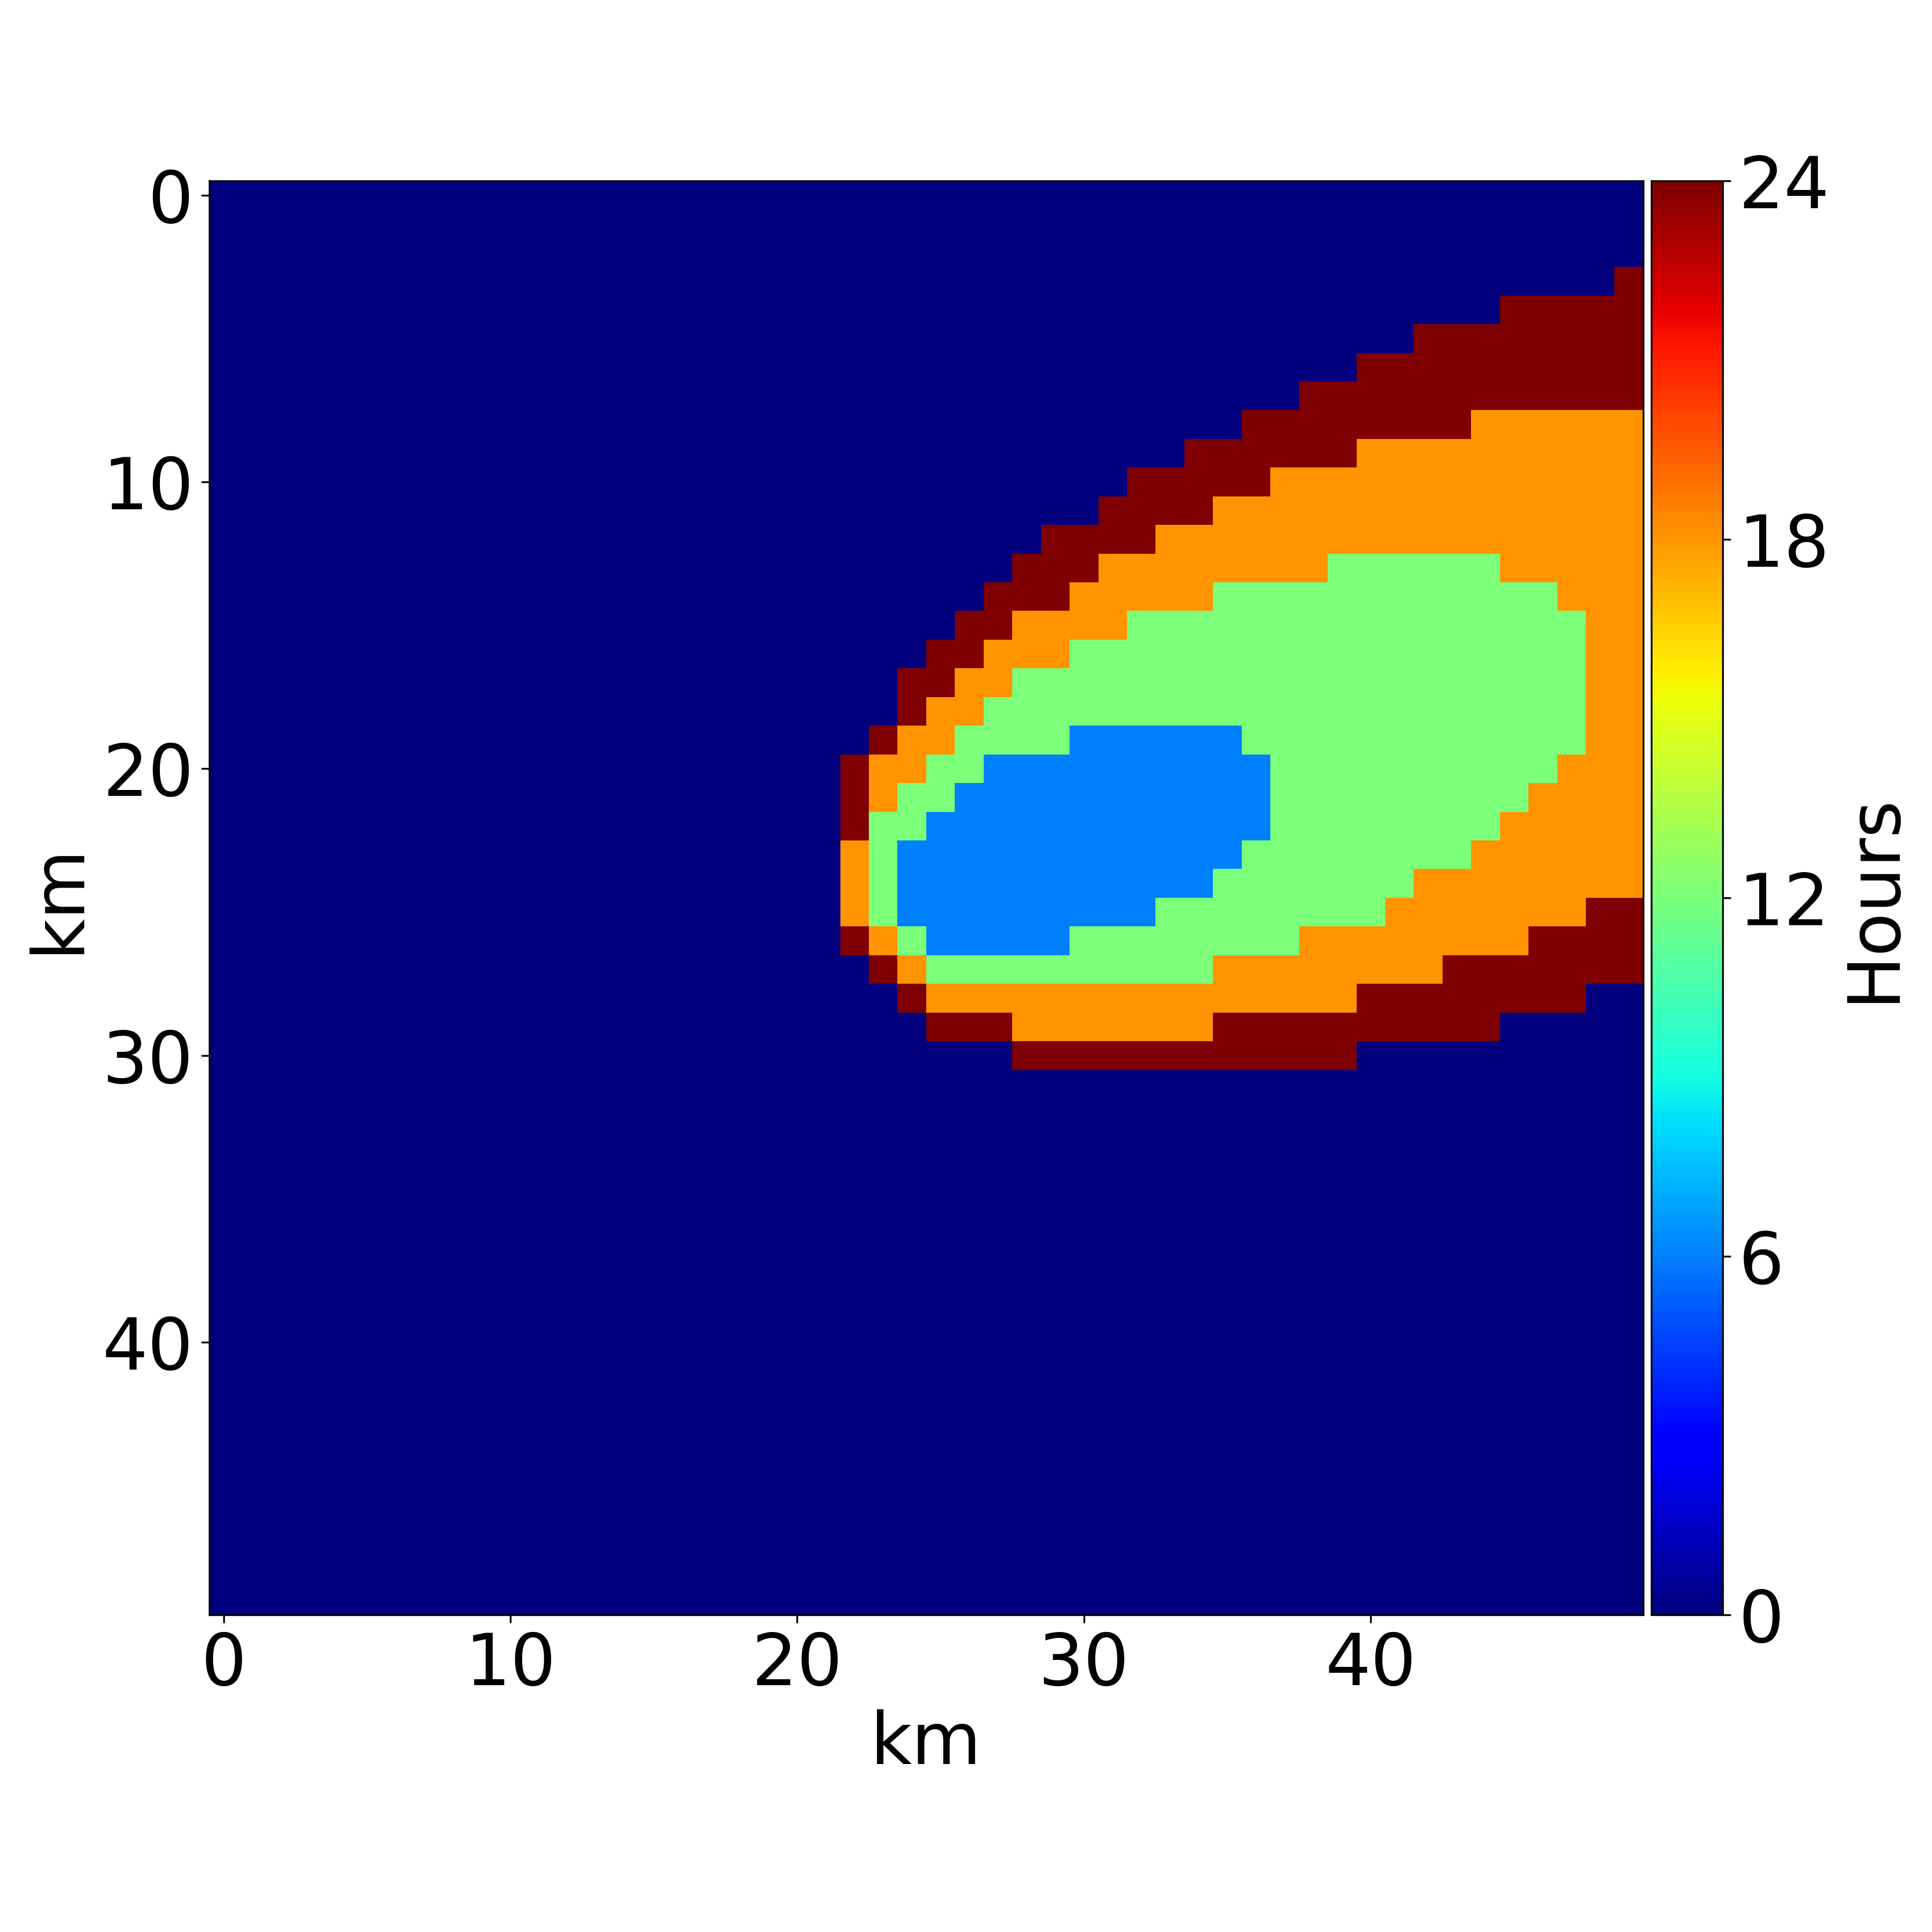
\includegraphics[height=0.25\textwidth]{timeAnalysis_simulation0.png}
	~
	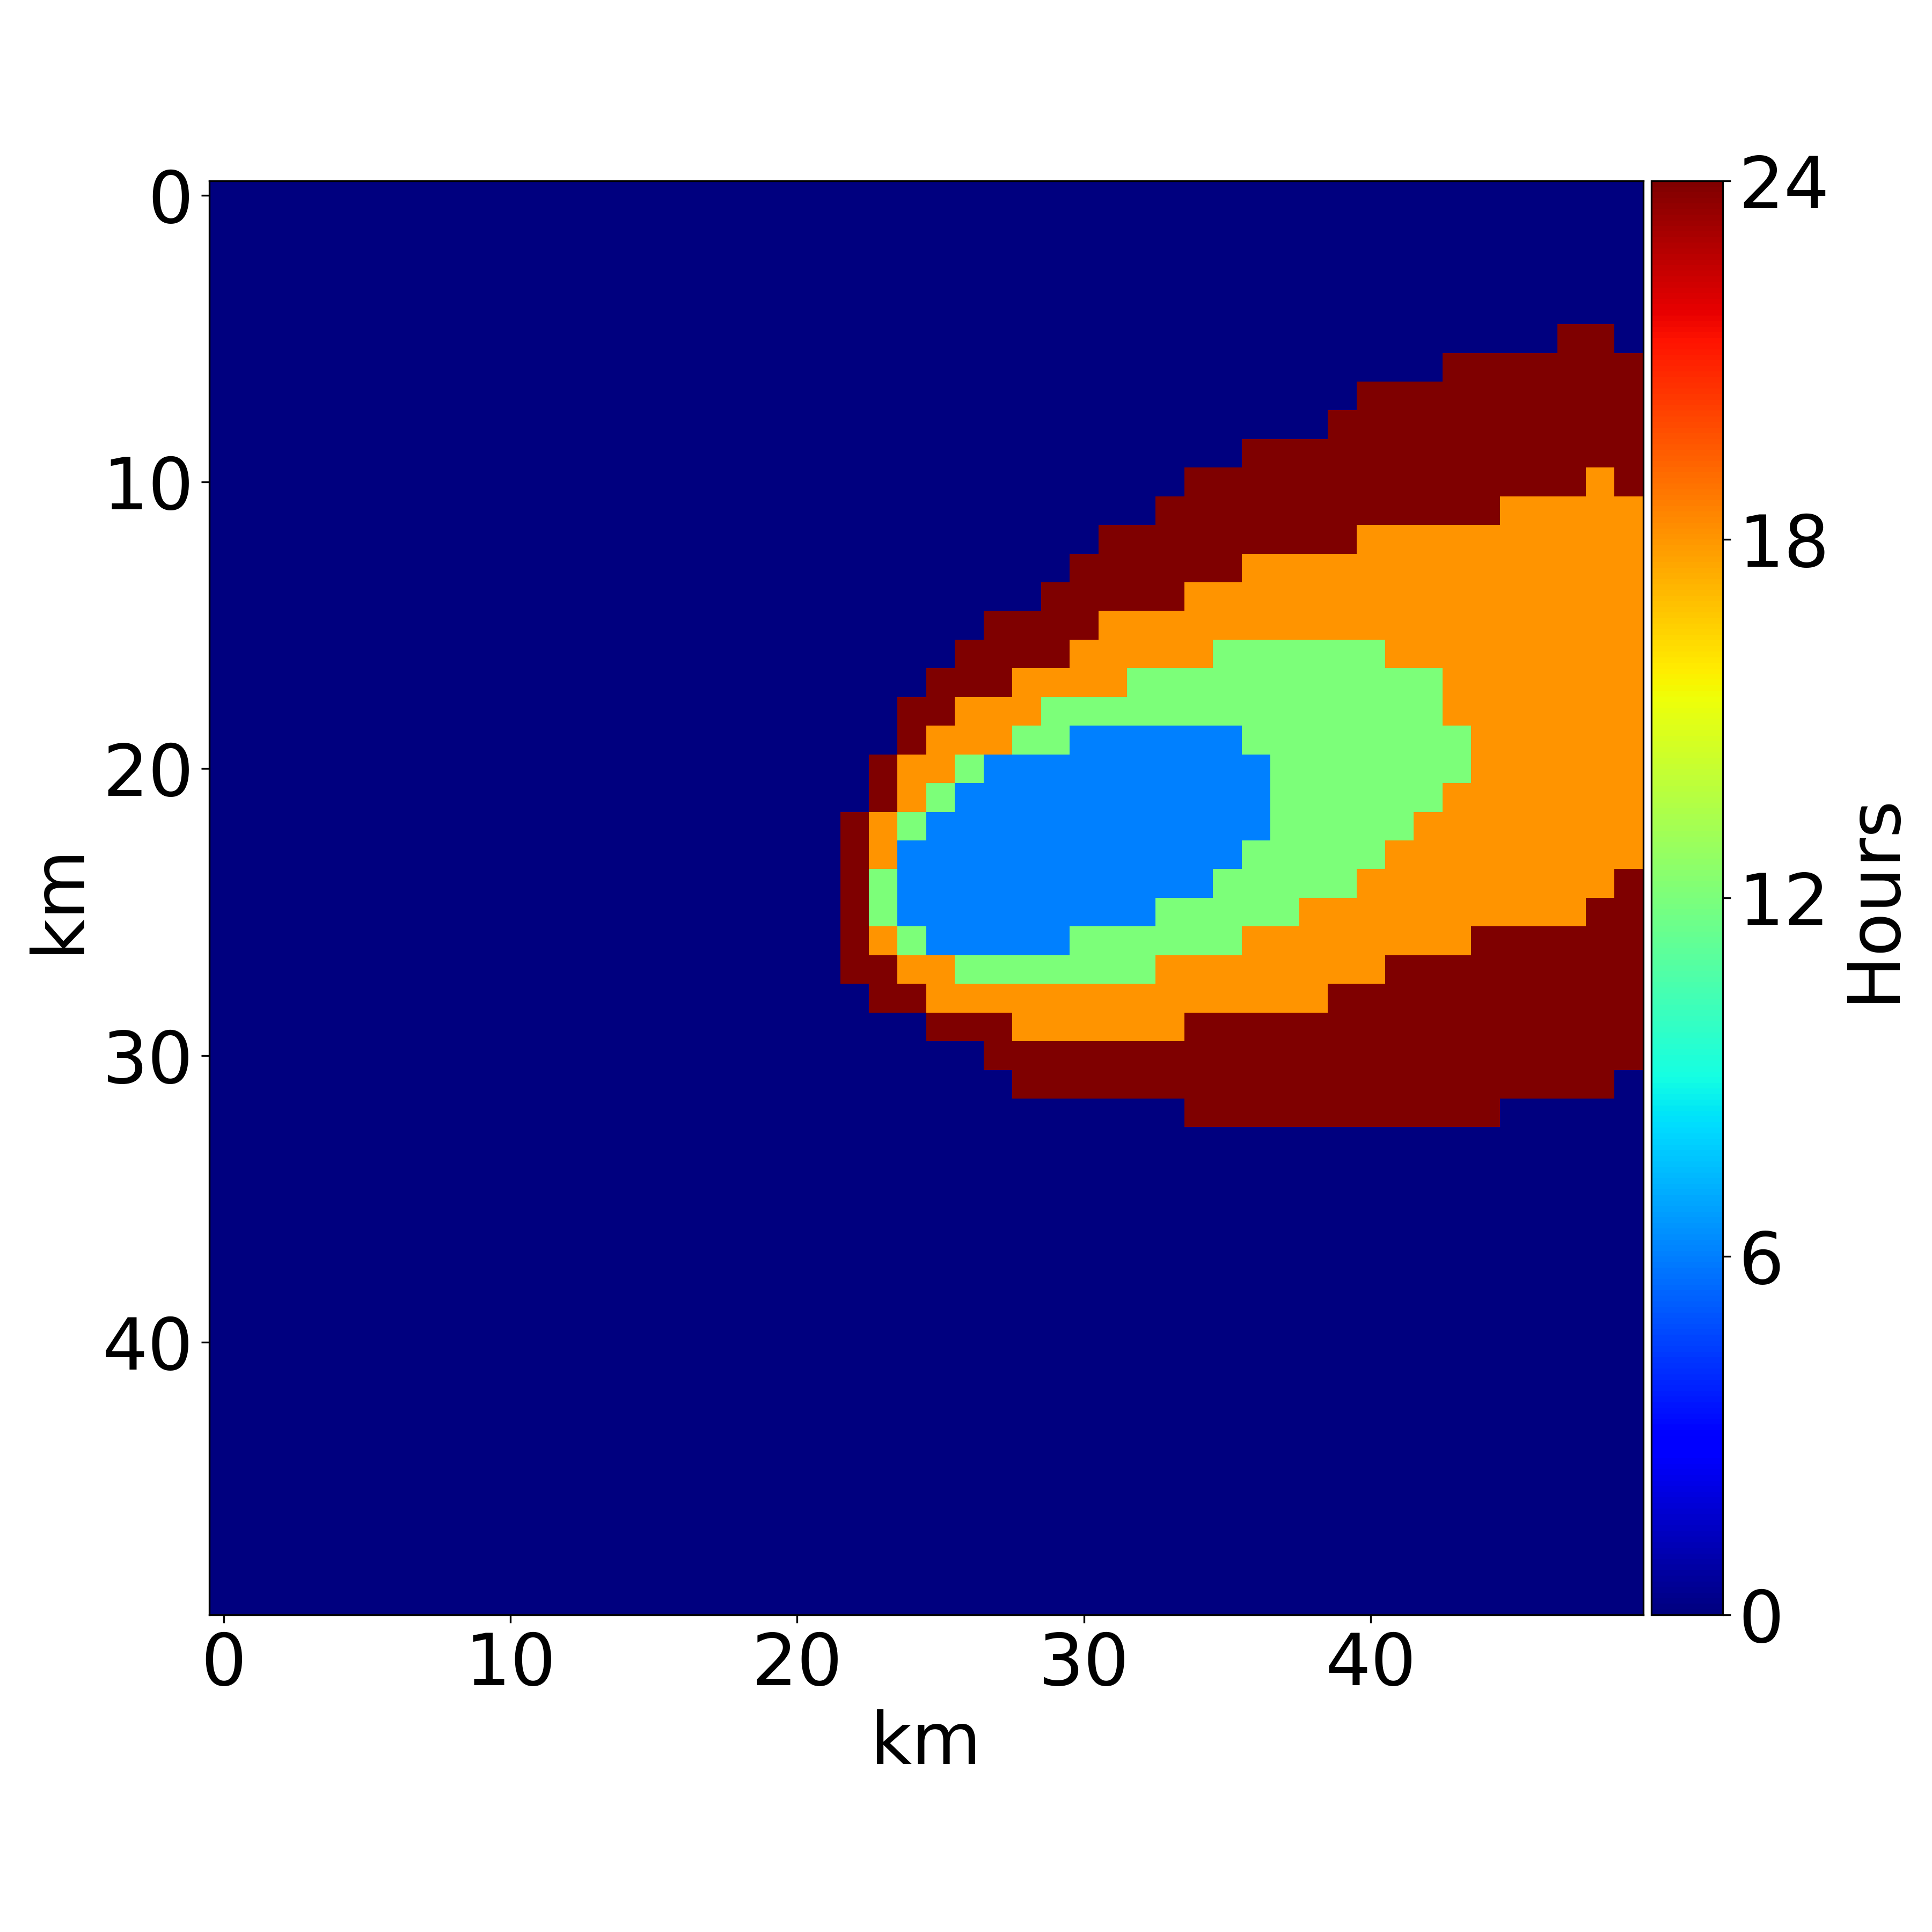
\includegraphics[height=0.25\textwidth]{timeAnalysis_network0.png}
	~
	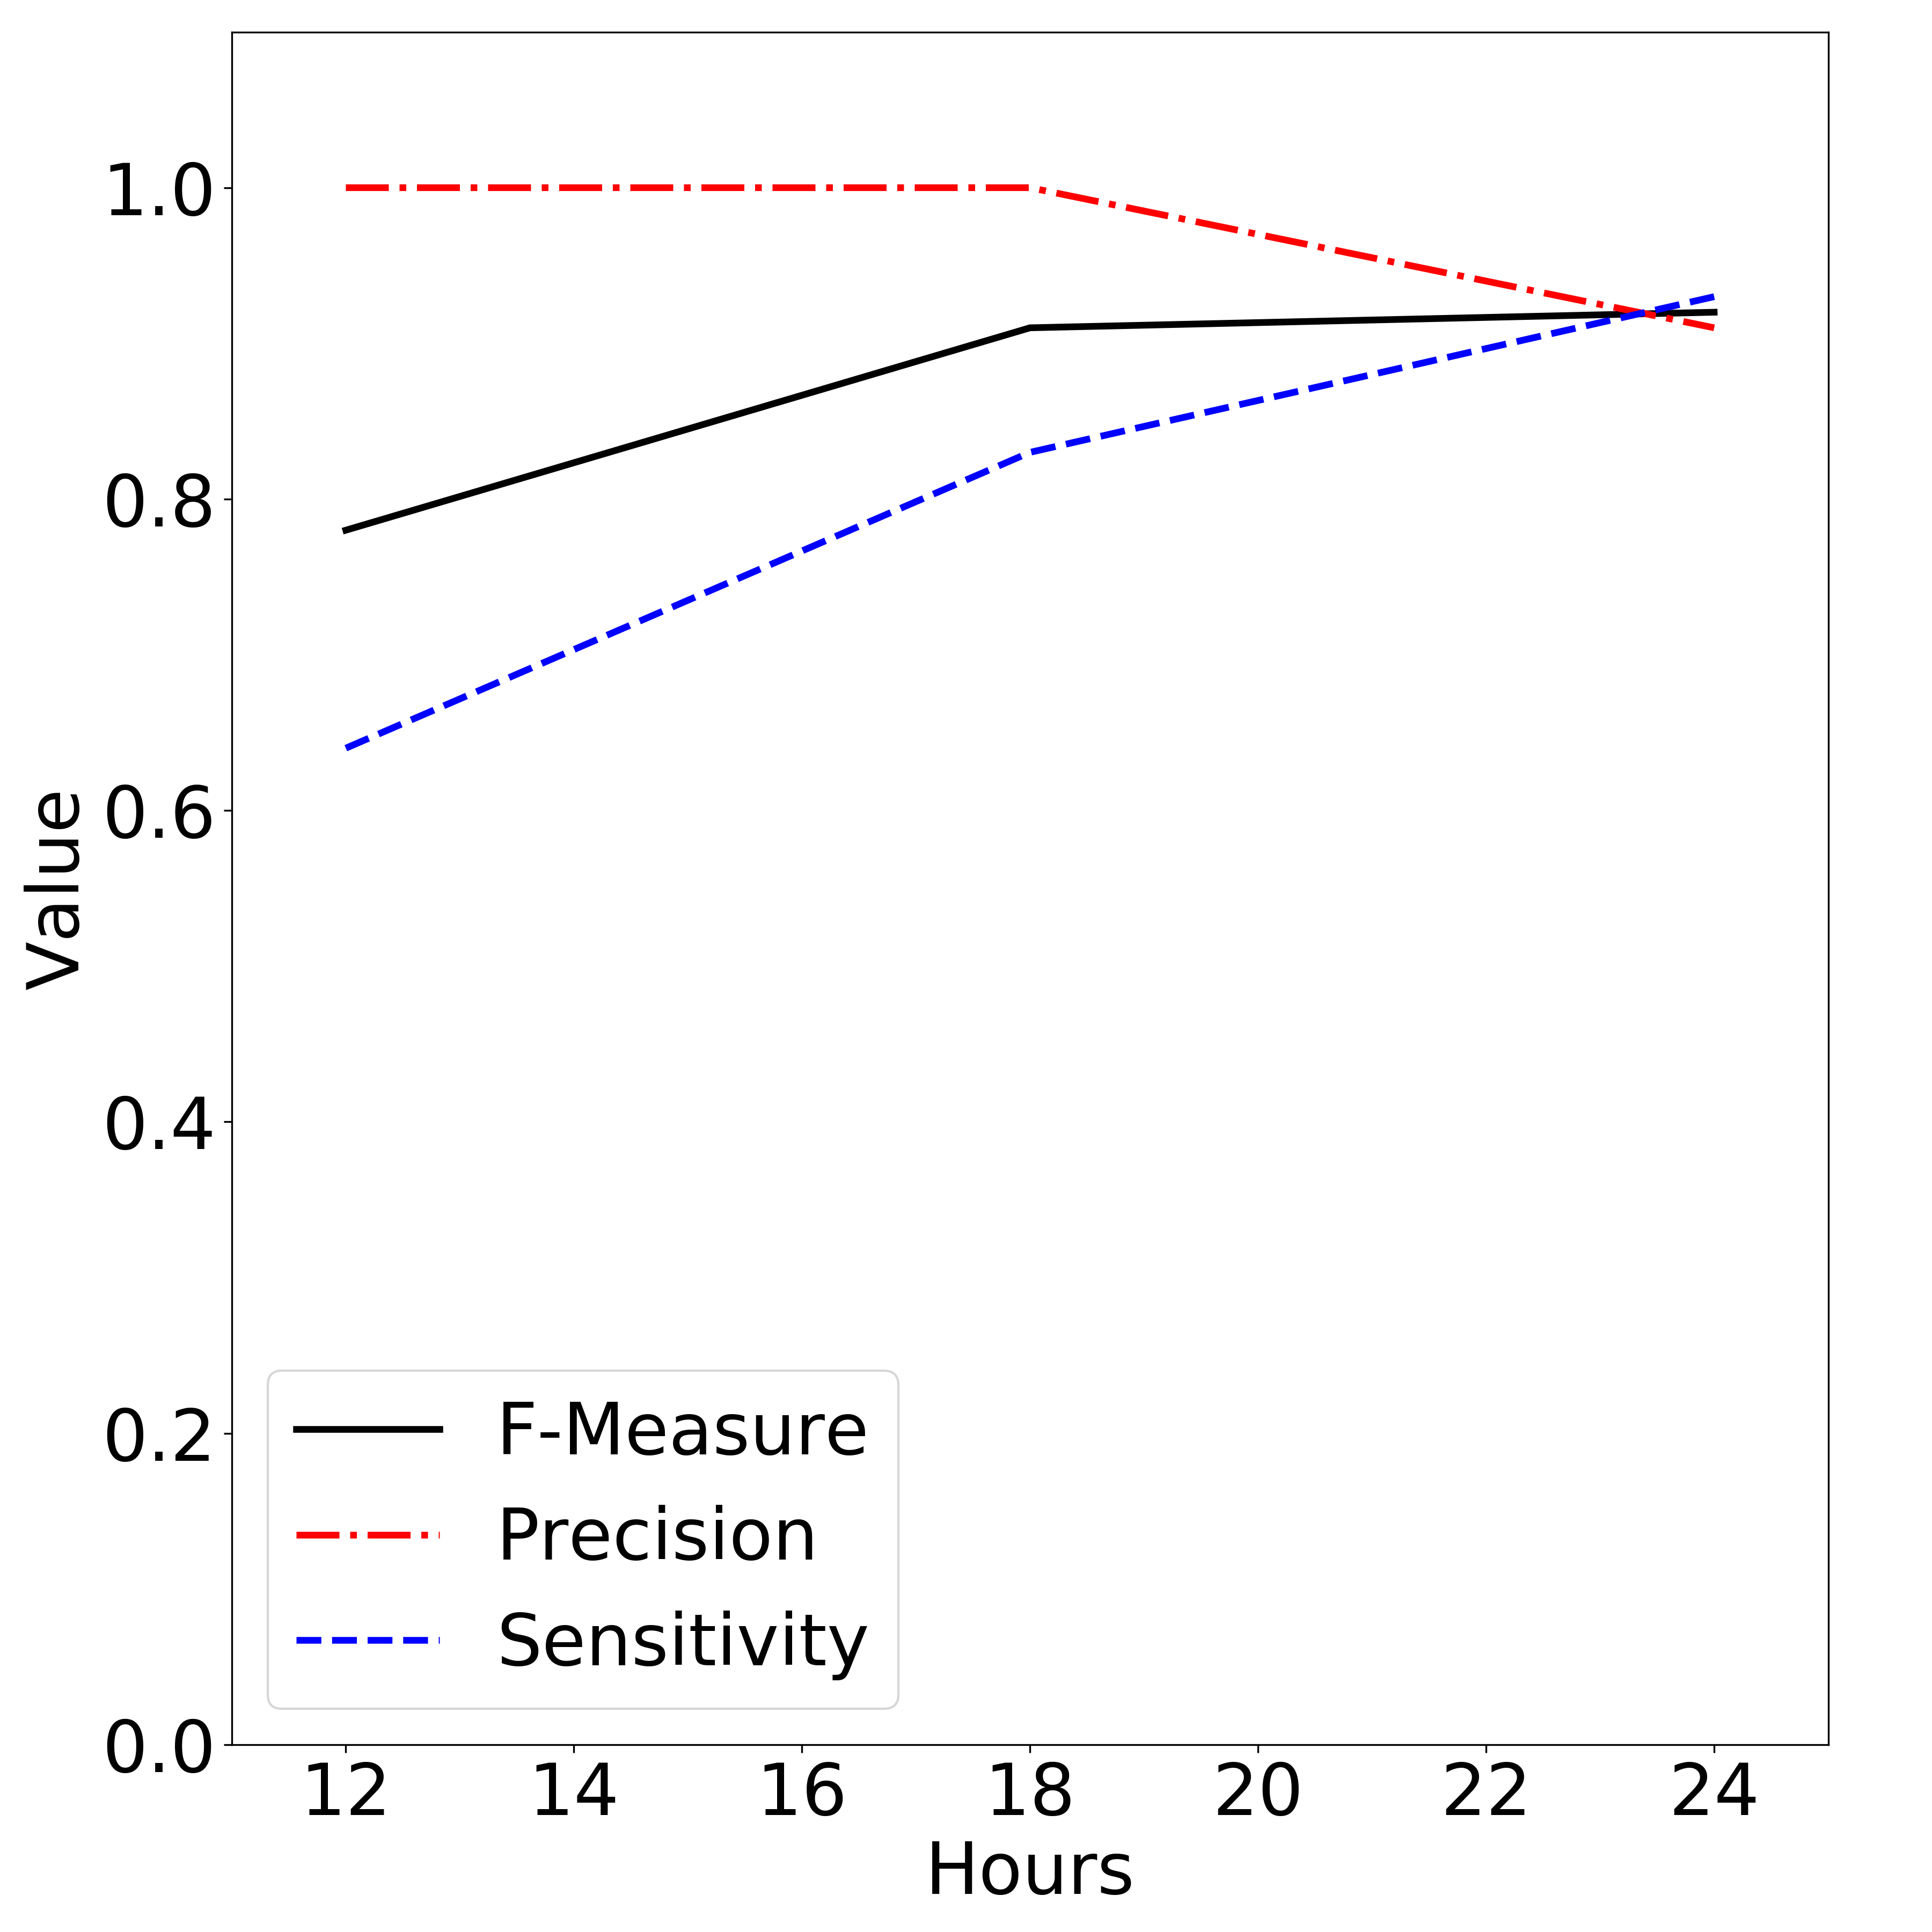
\includegraphics[height=0.25\textwidth]{timeAnalysis_fmeasure0.png}
	\\
	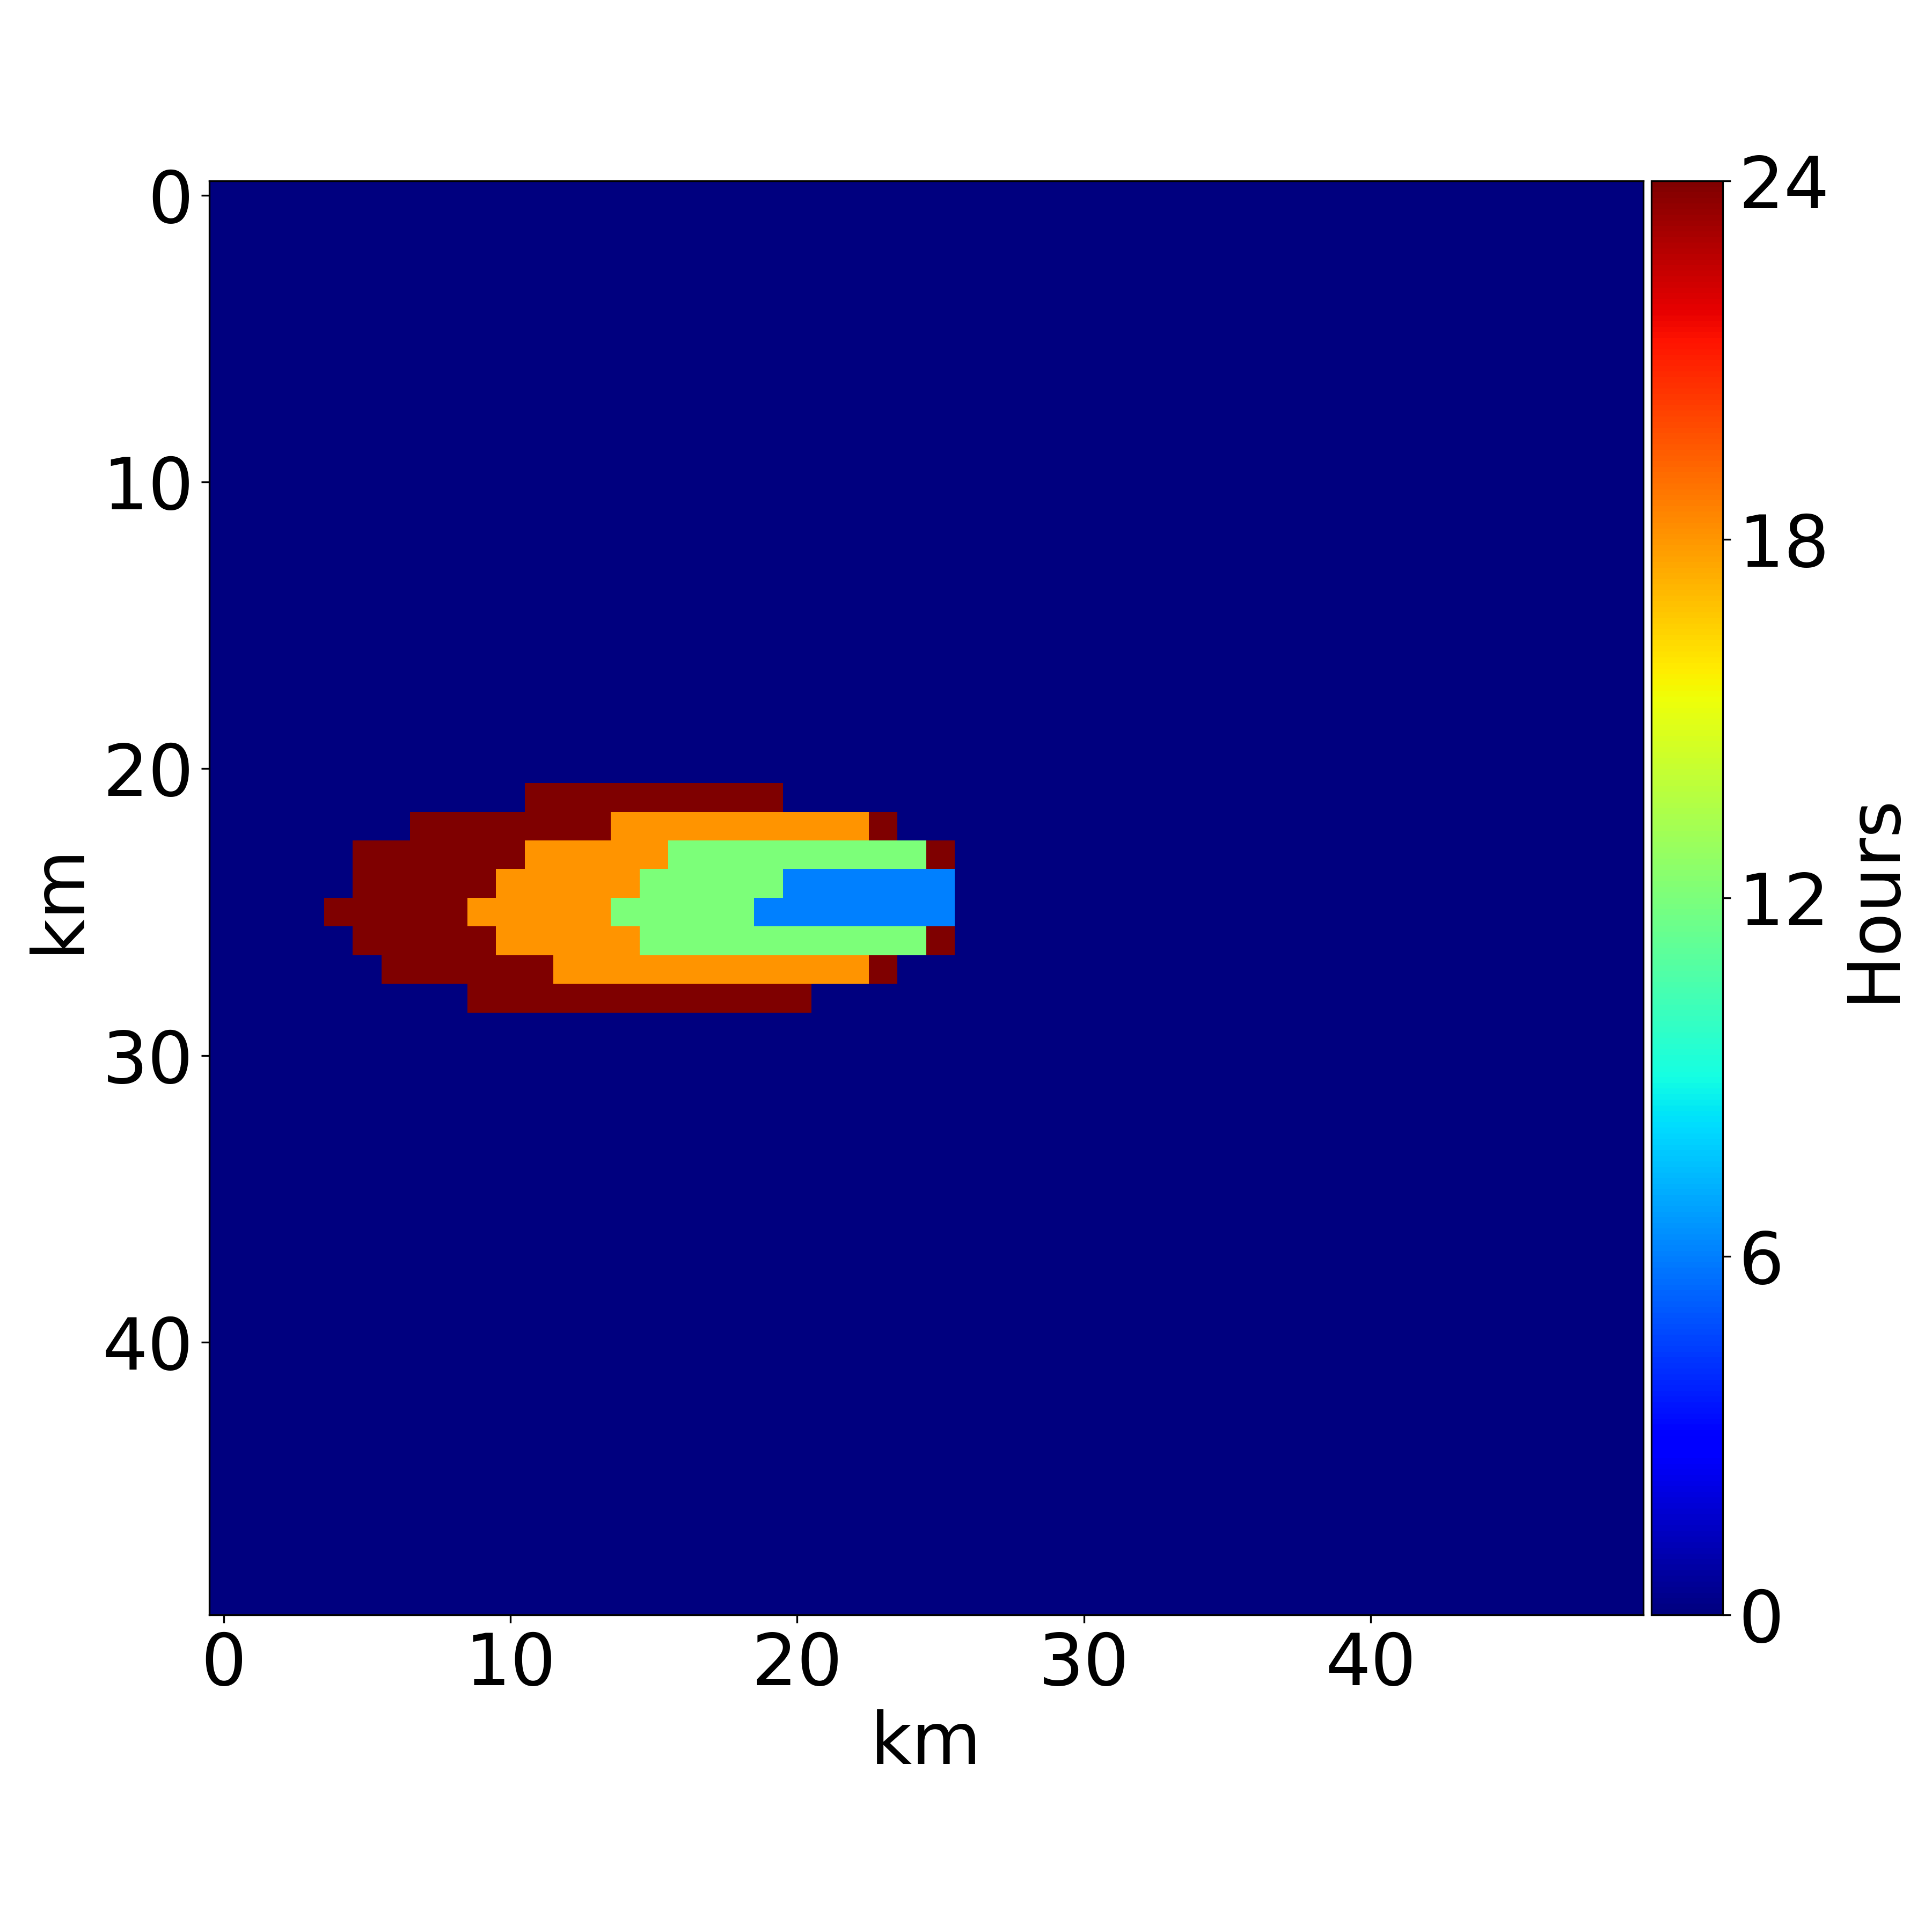
\includegraphics[height=0.25\textwidth]{timeAnalysis_simulation1.png}
	~
	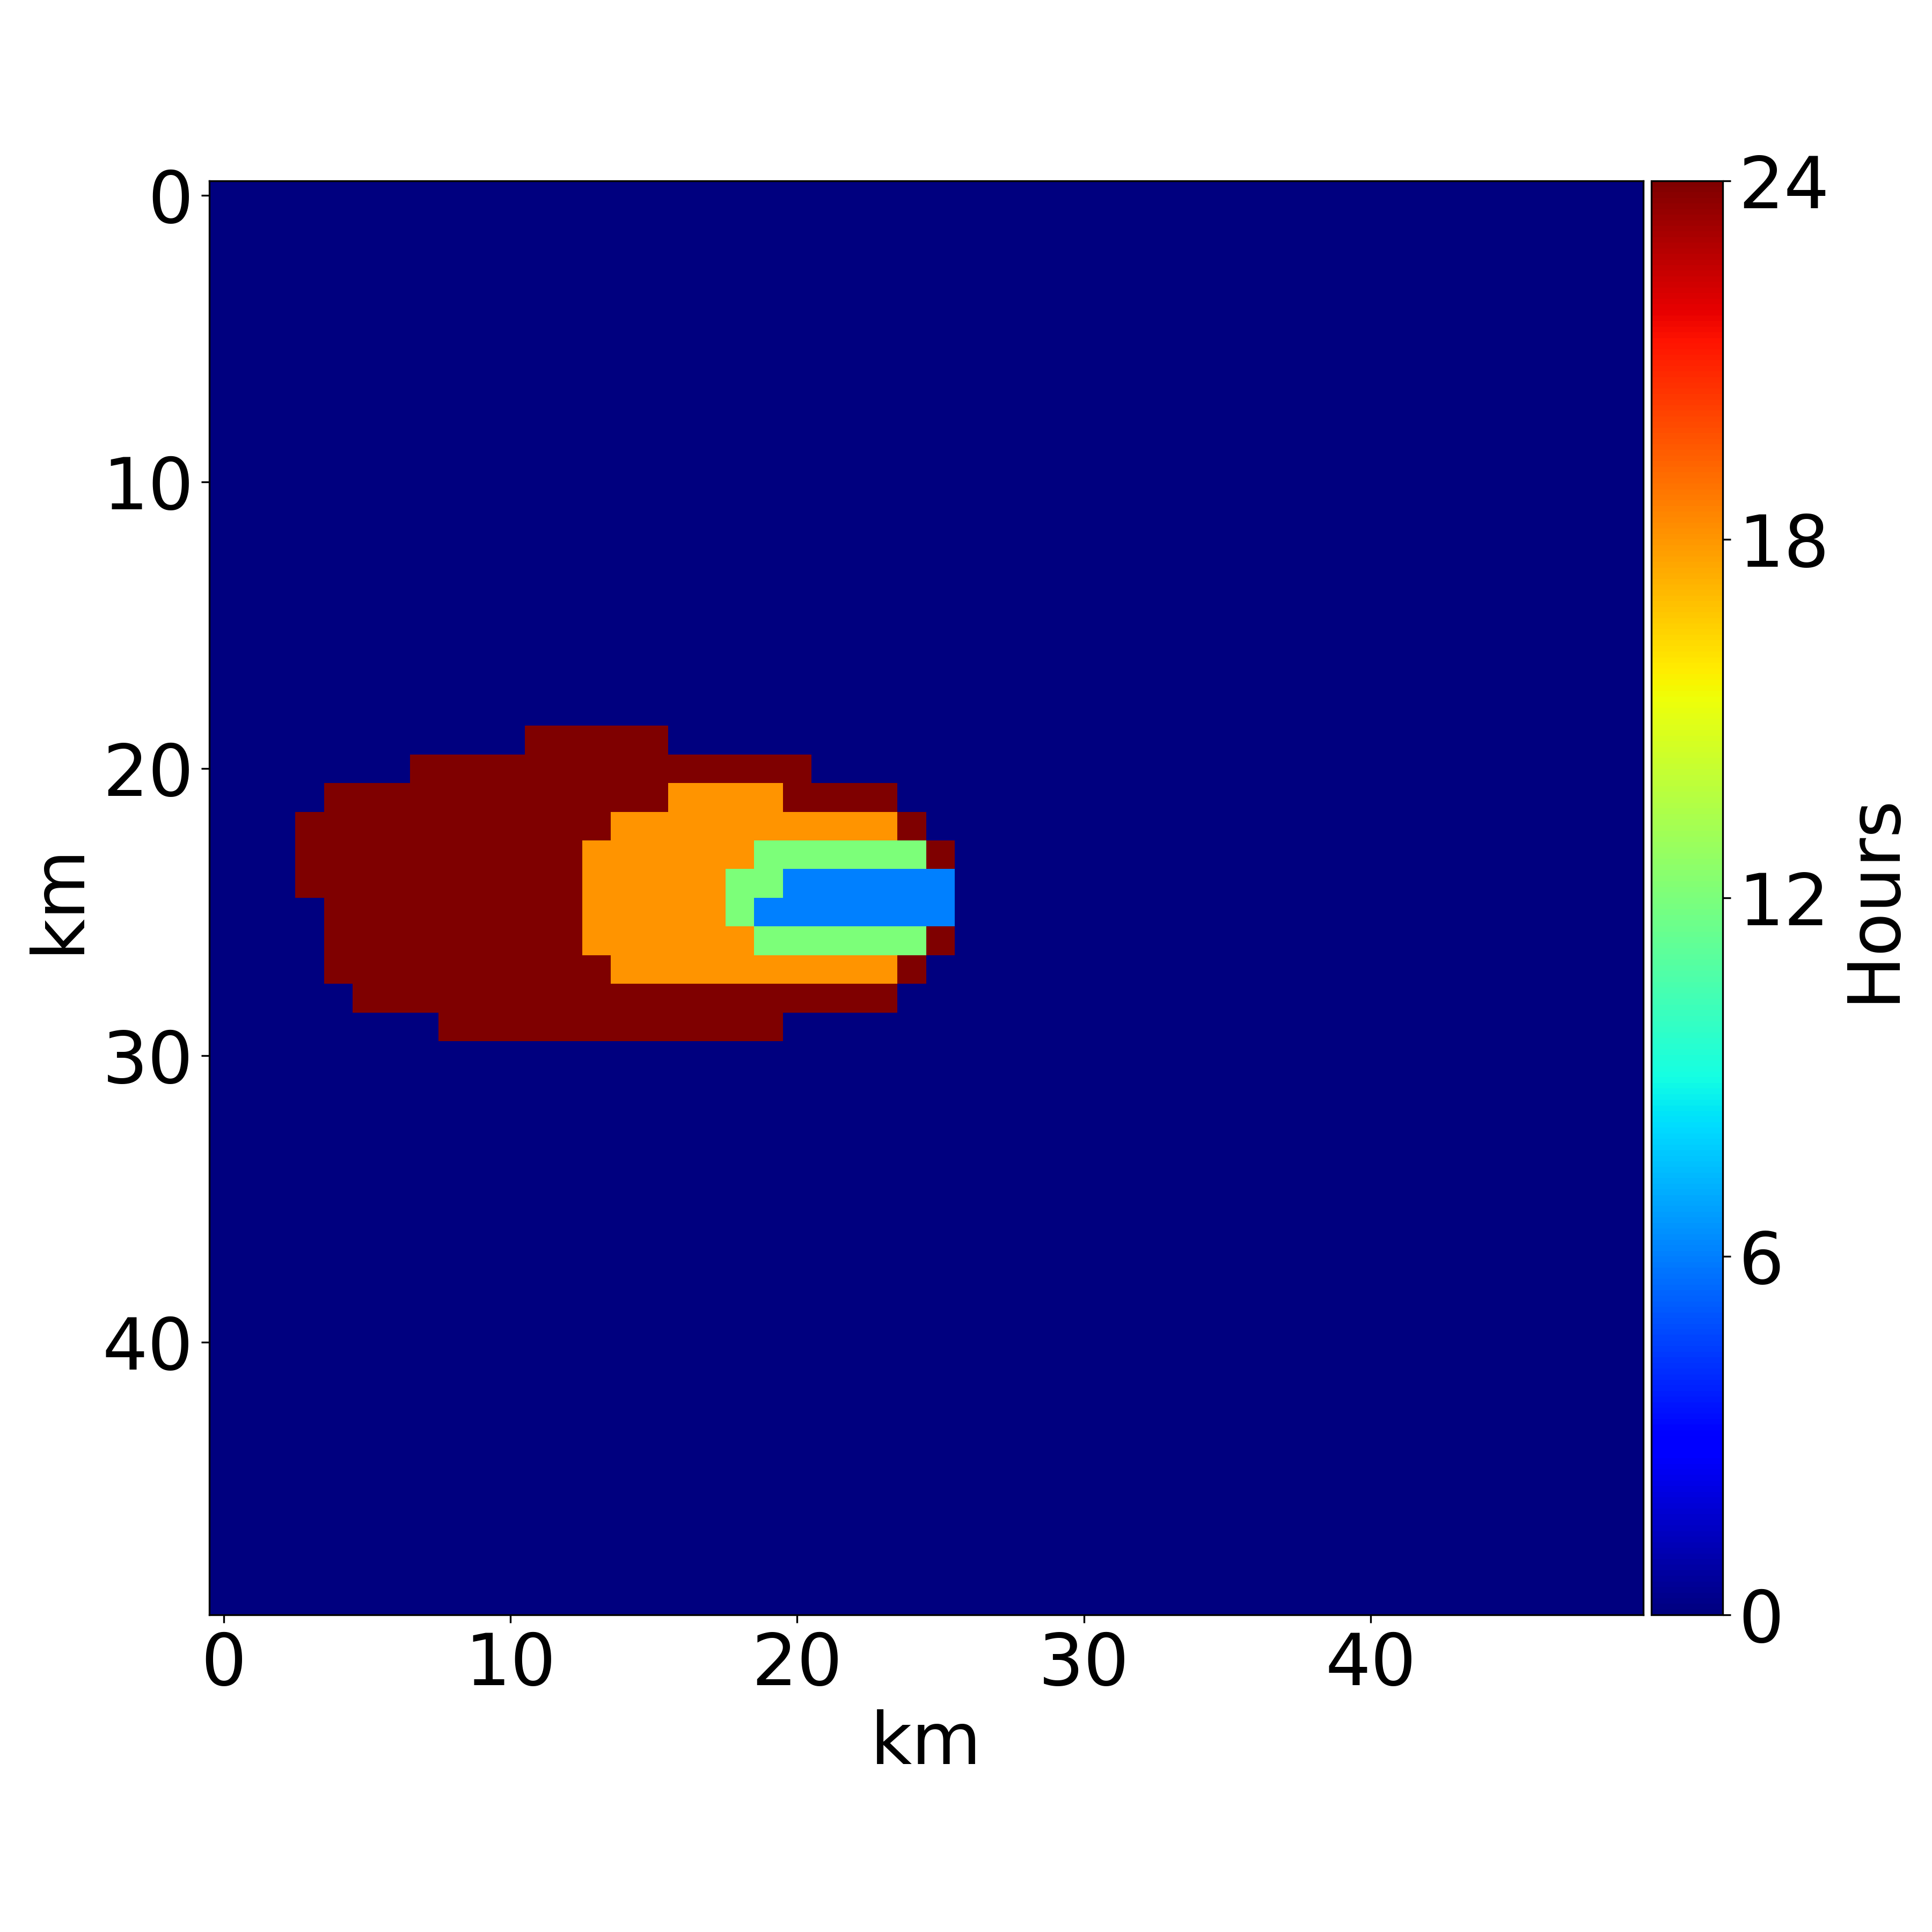
\includegraphics[height=0.25\textwidth]{timeAnalysis_network1.png}
	~
	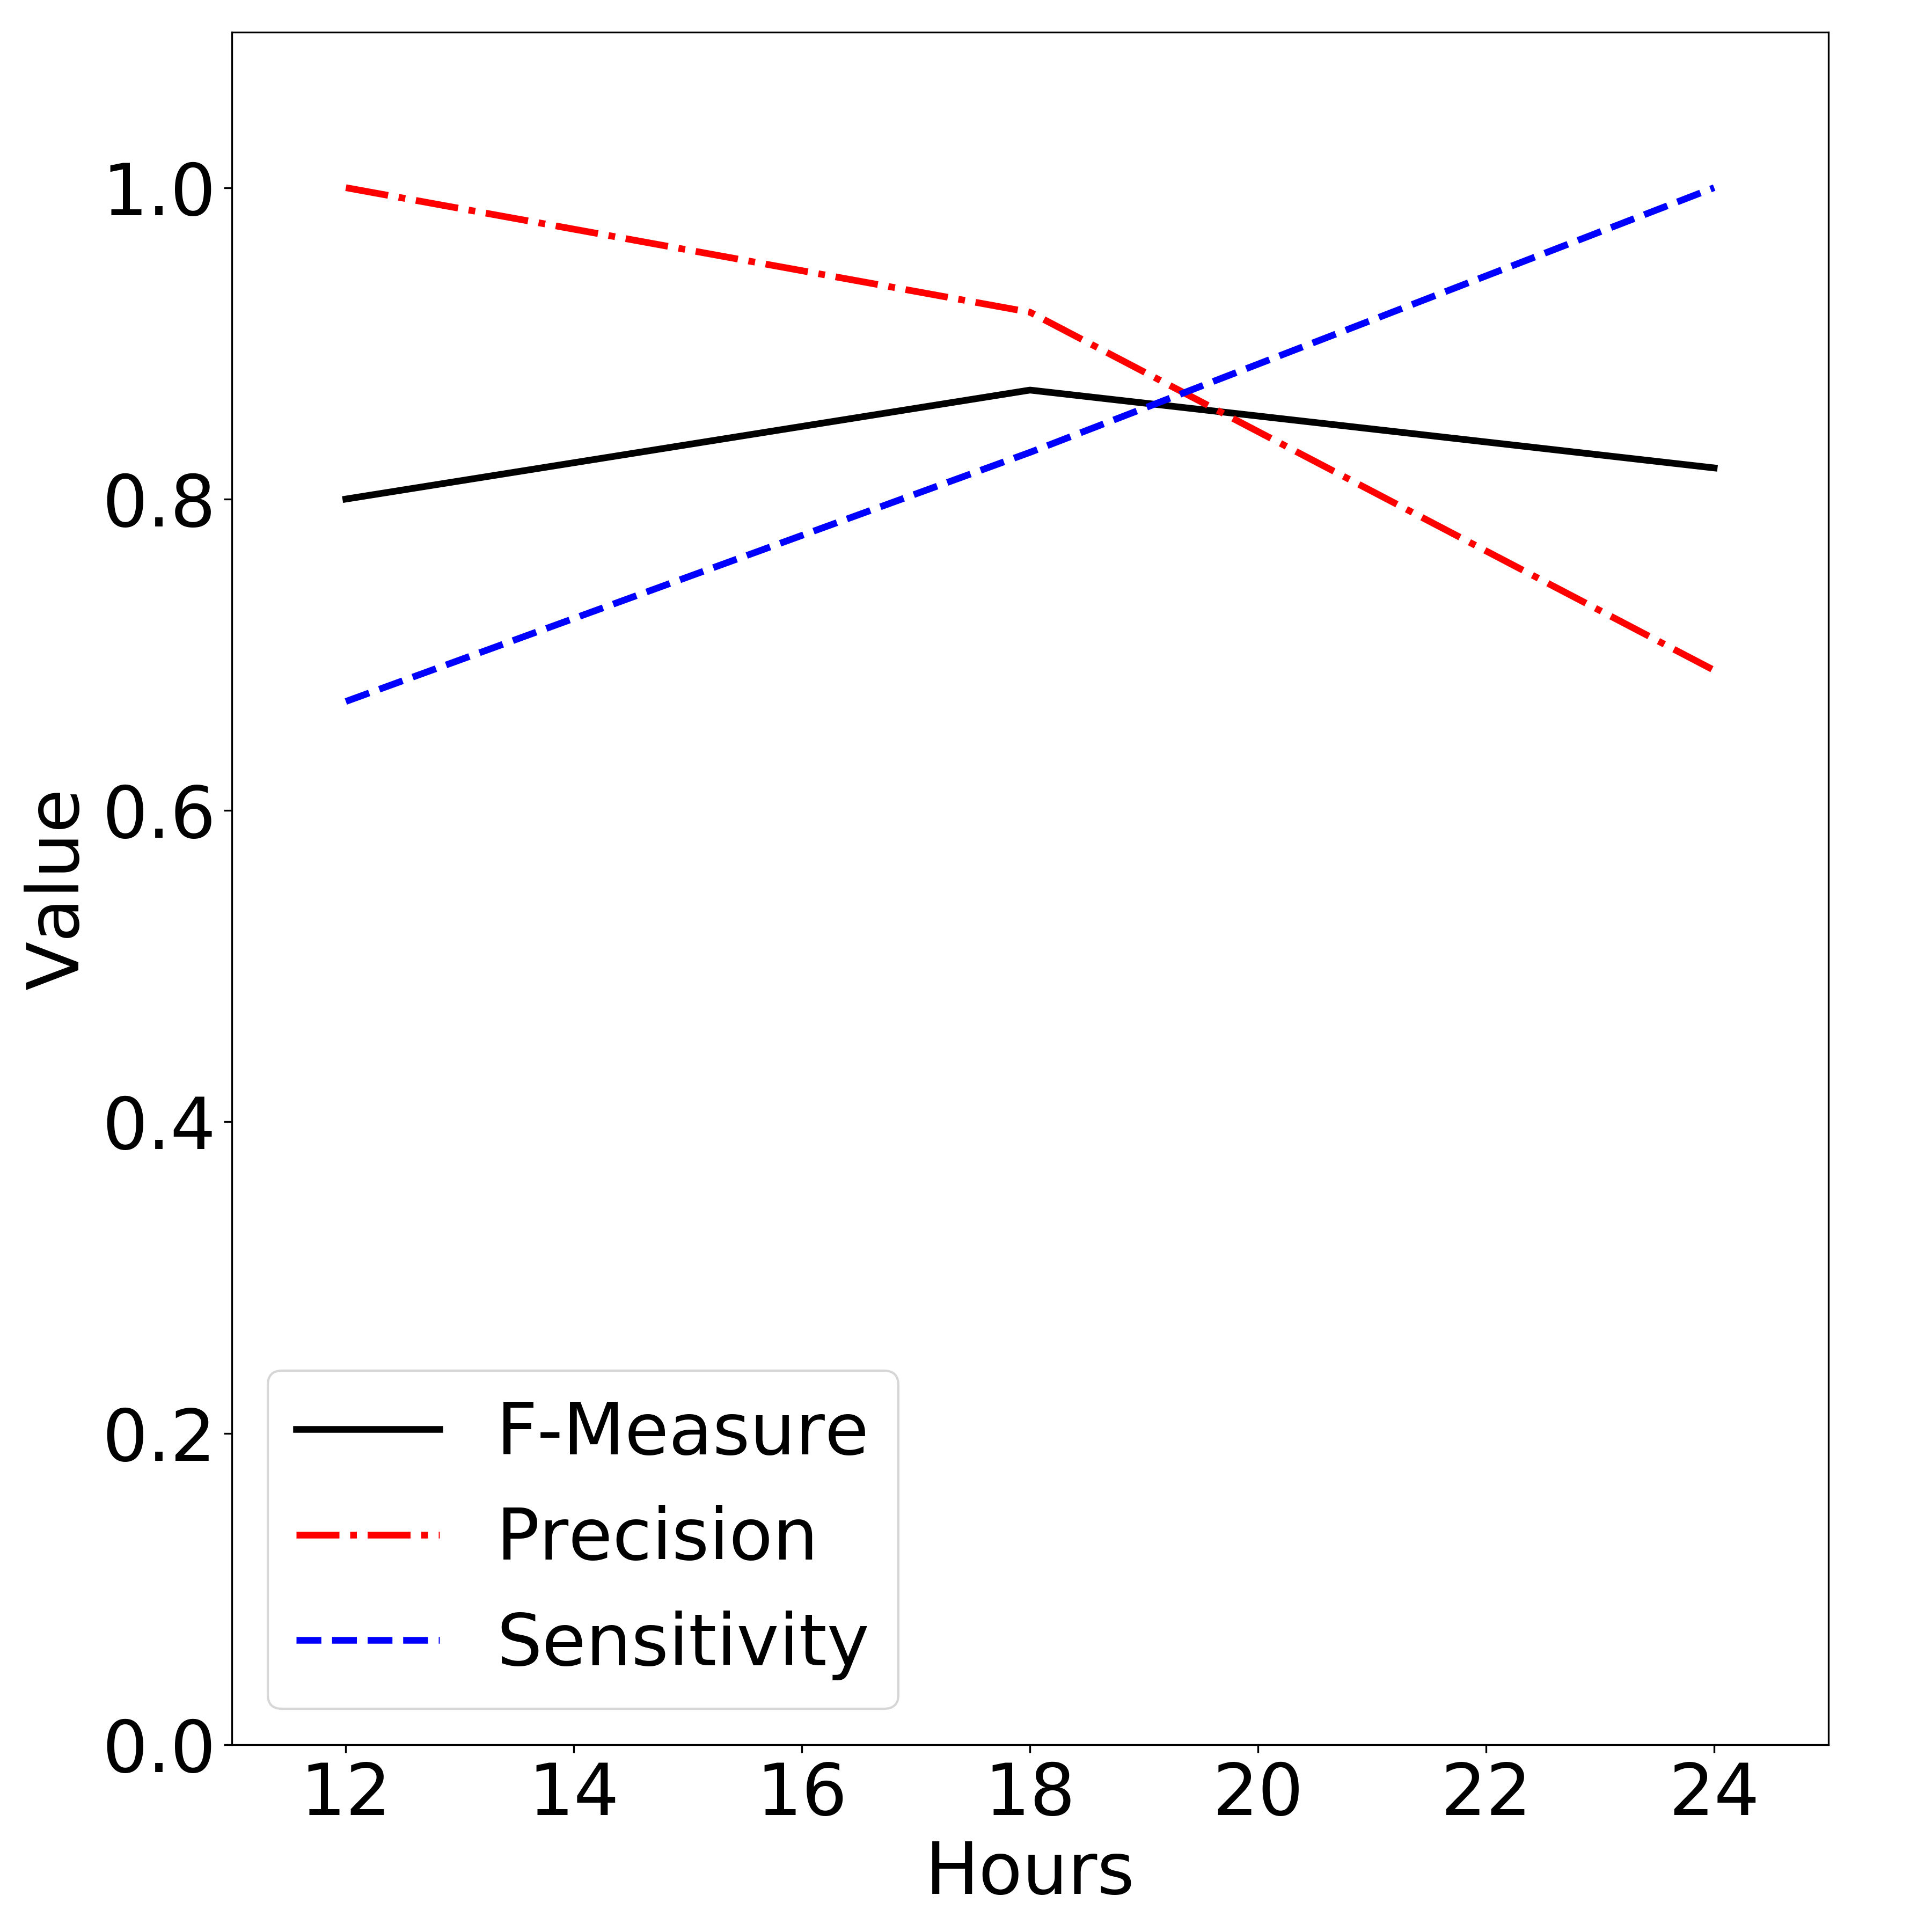
\includegraphics[height=0.25\textwidth]{timeAnalysis_fmeasure1.png}
	\\
	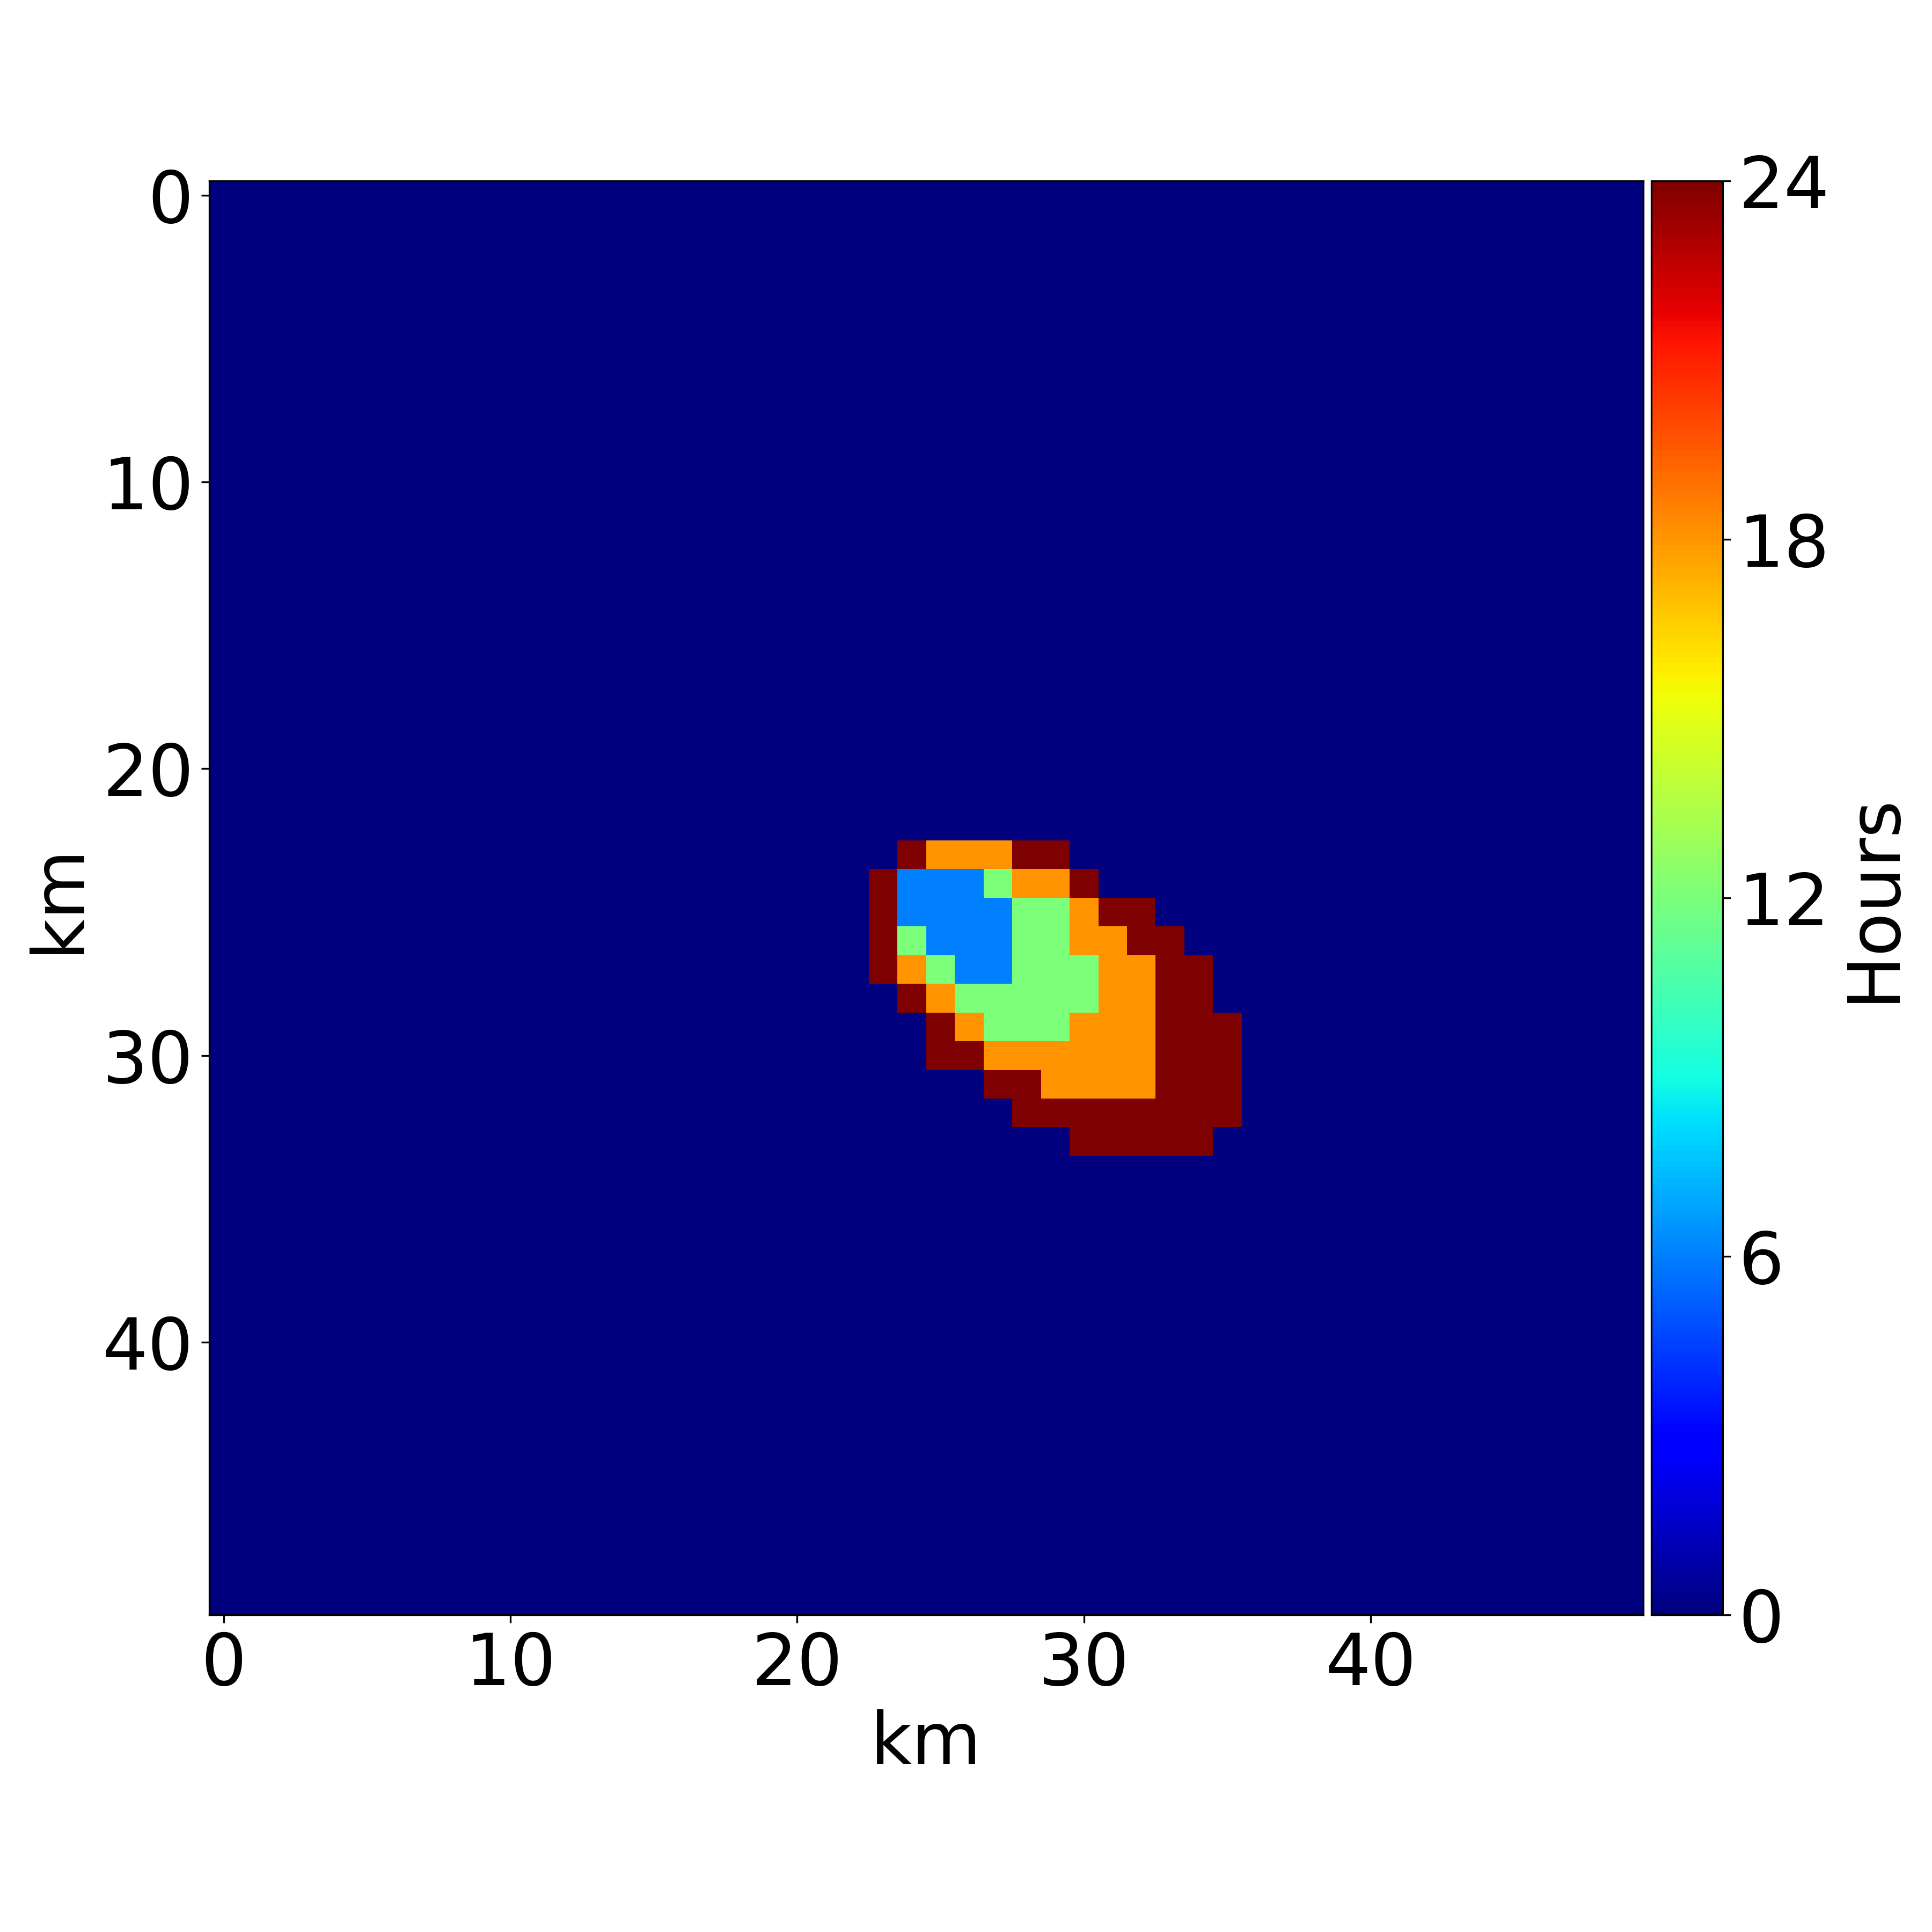
\includegraphics[height=0.25\textwidth]{timeAnalysis_simulation2.png}
	~
	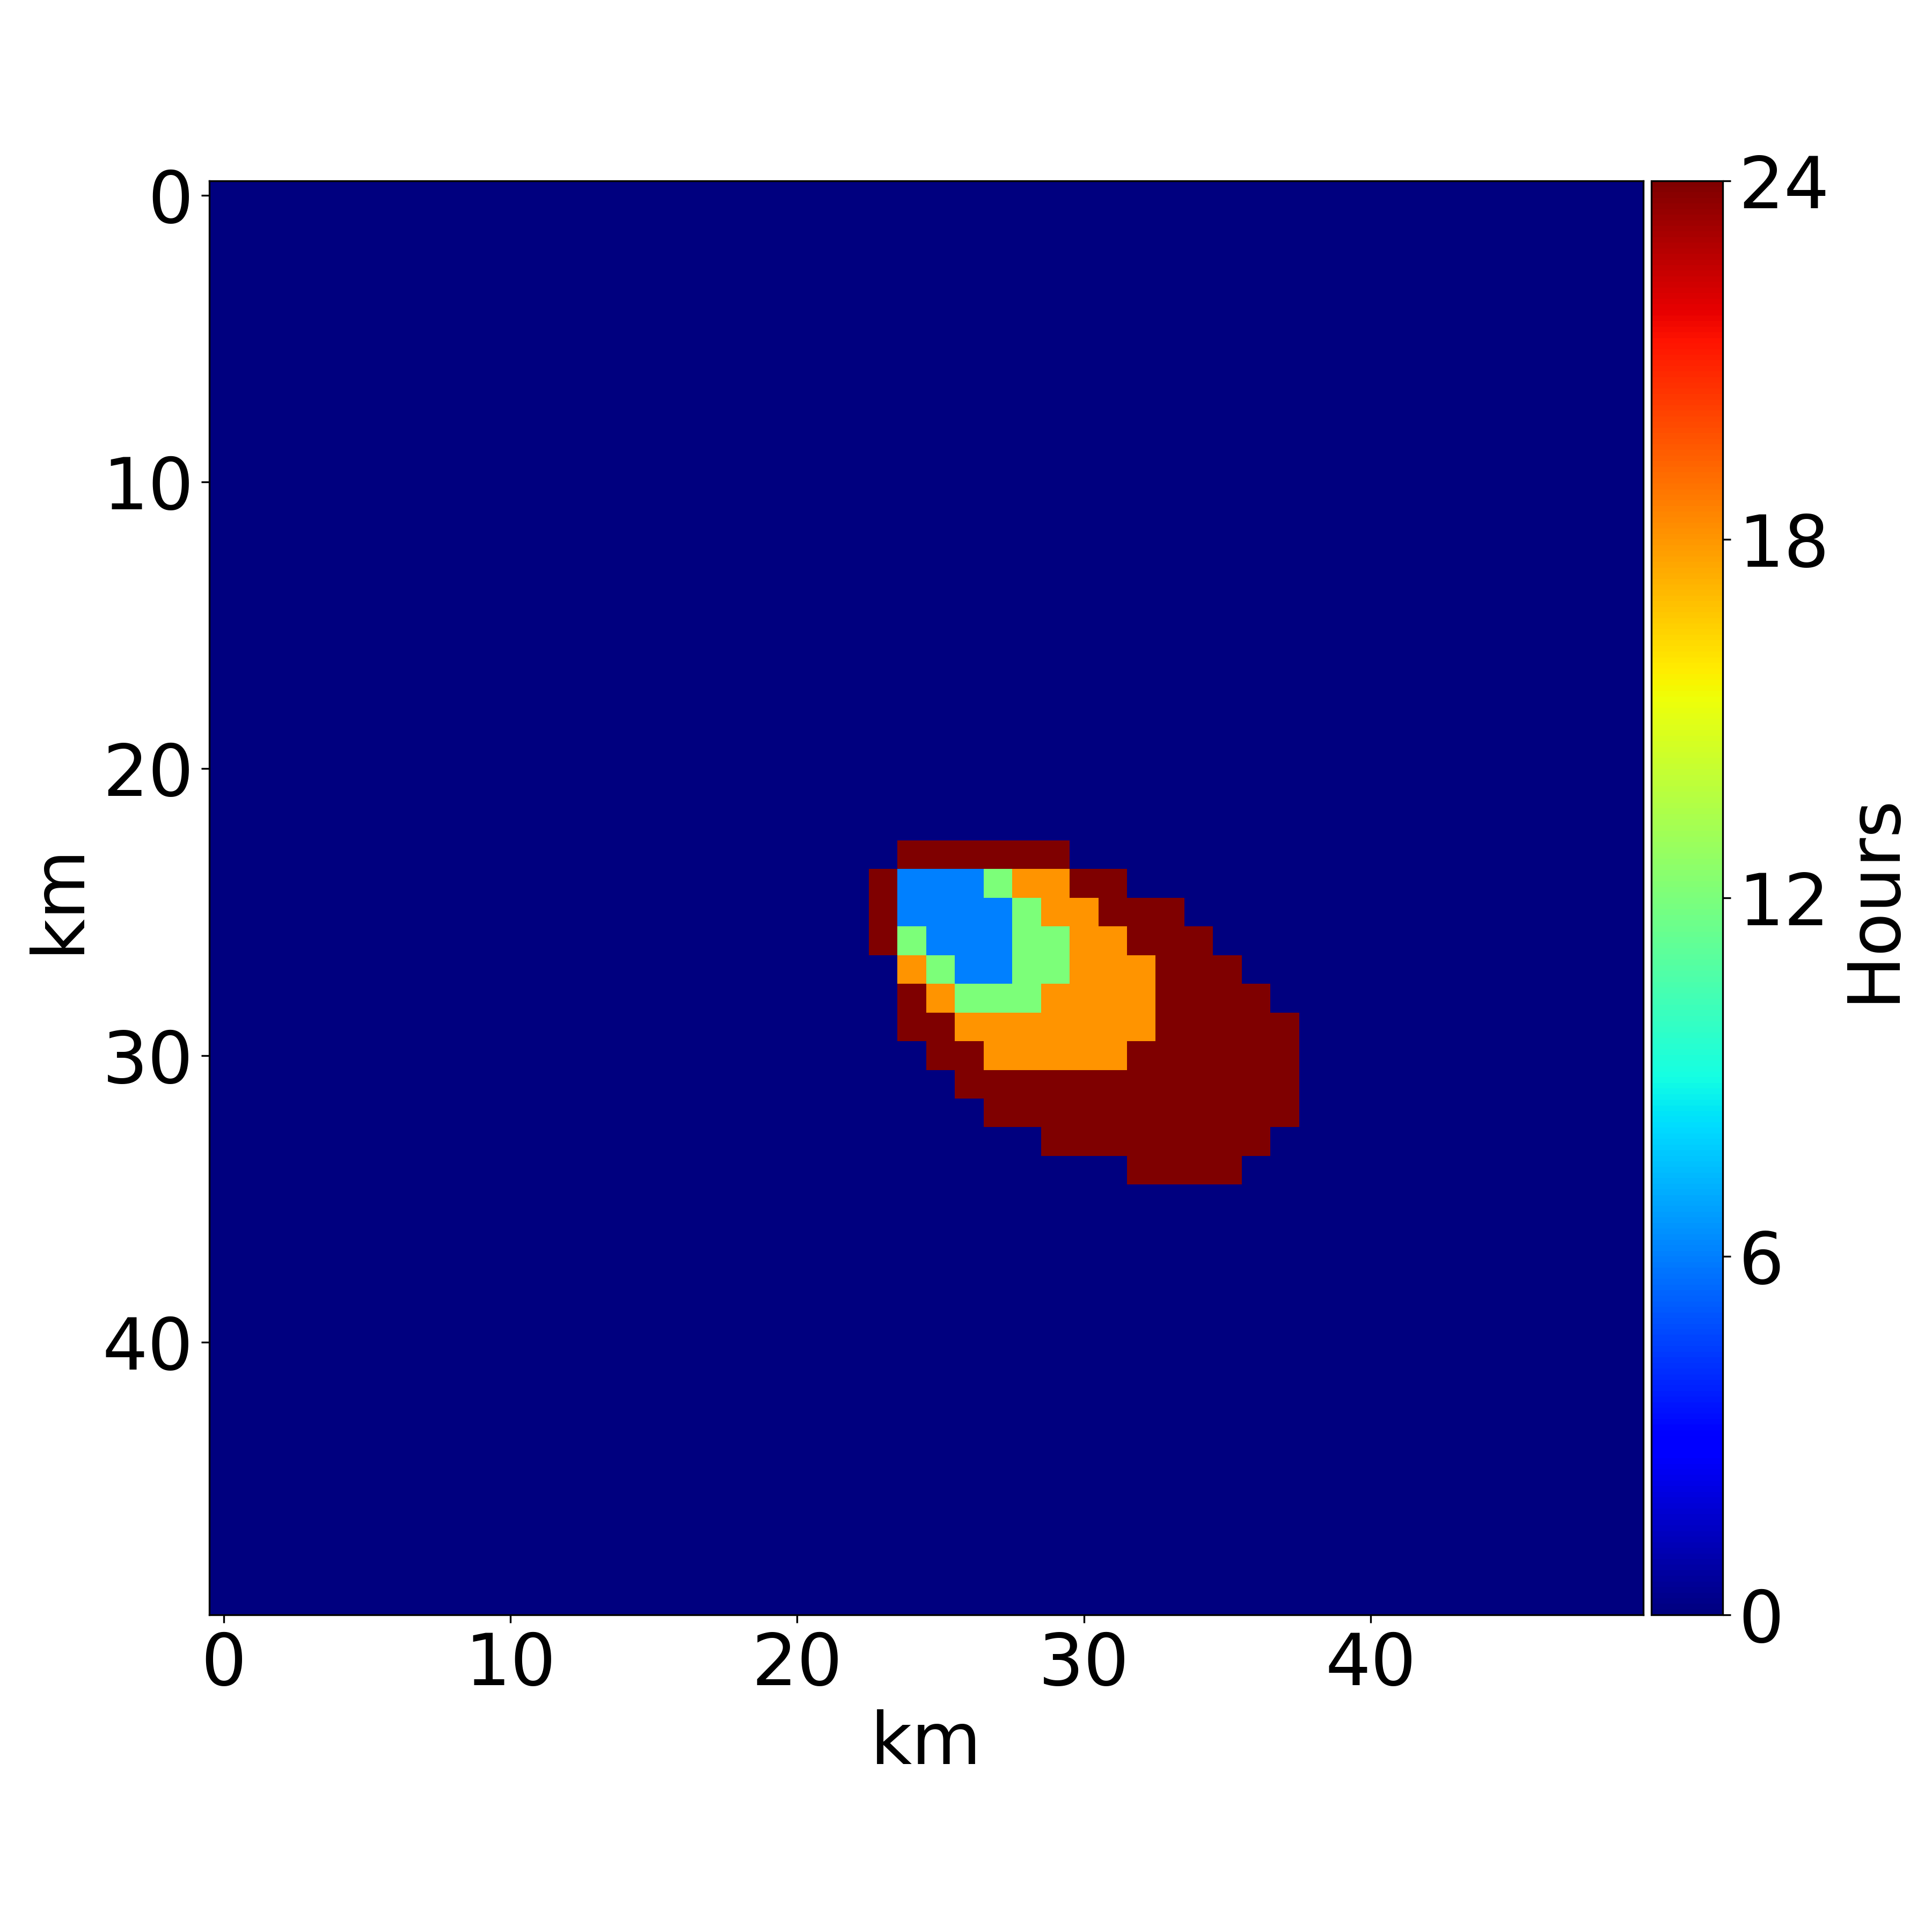
\includegraphics[height=0.25\textwidth]{timeAnalysis_network2.png}
	~
	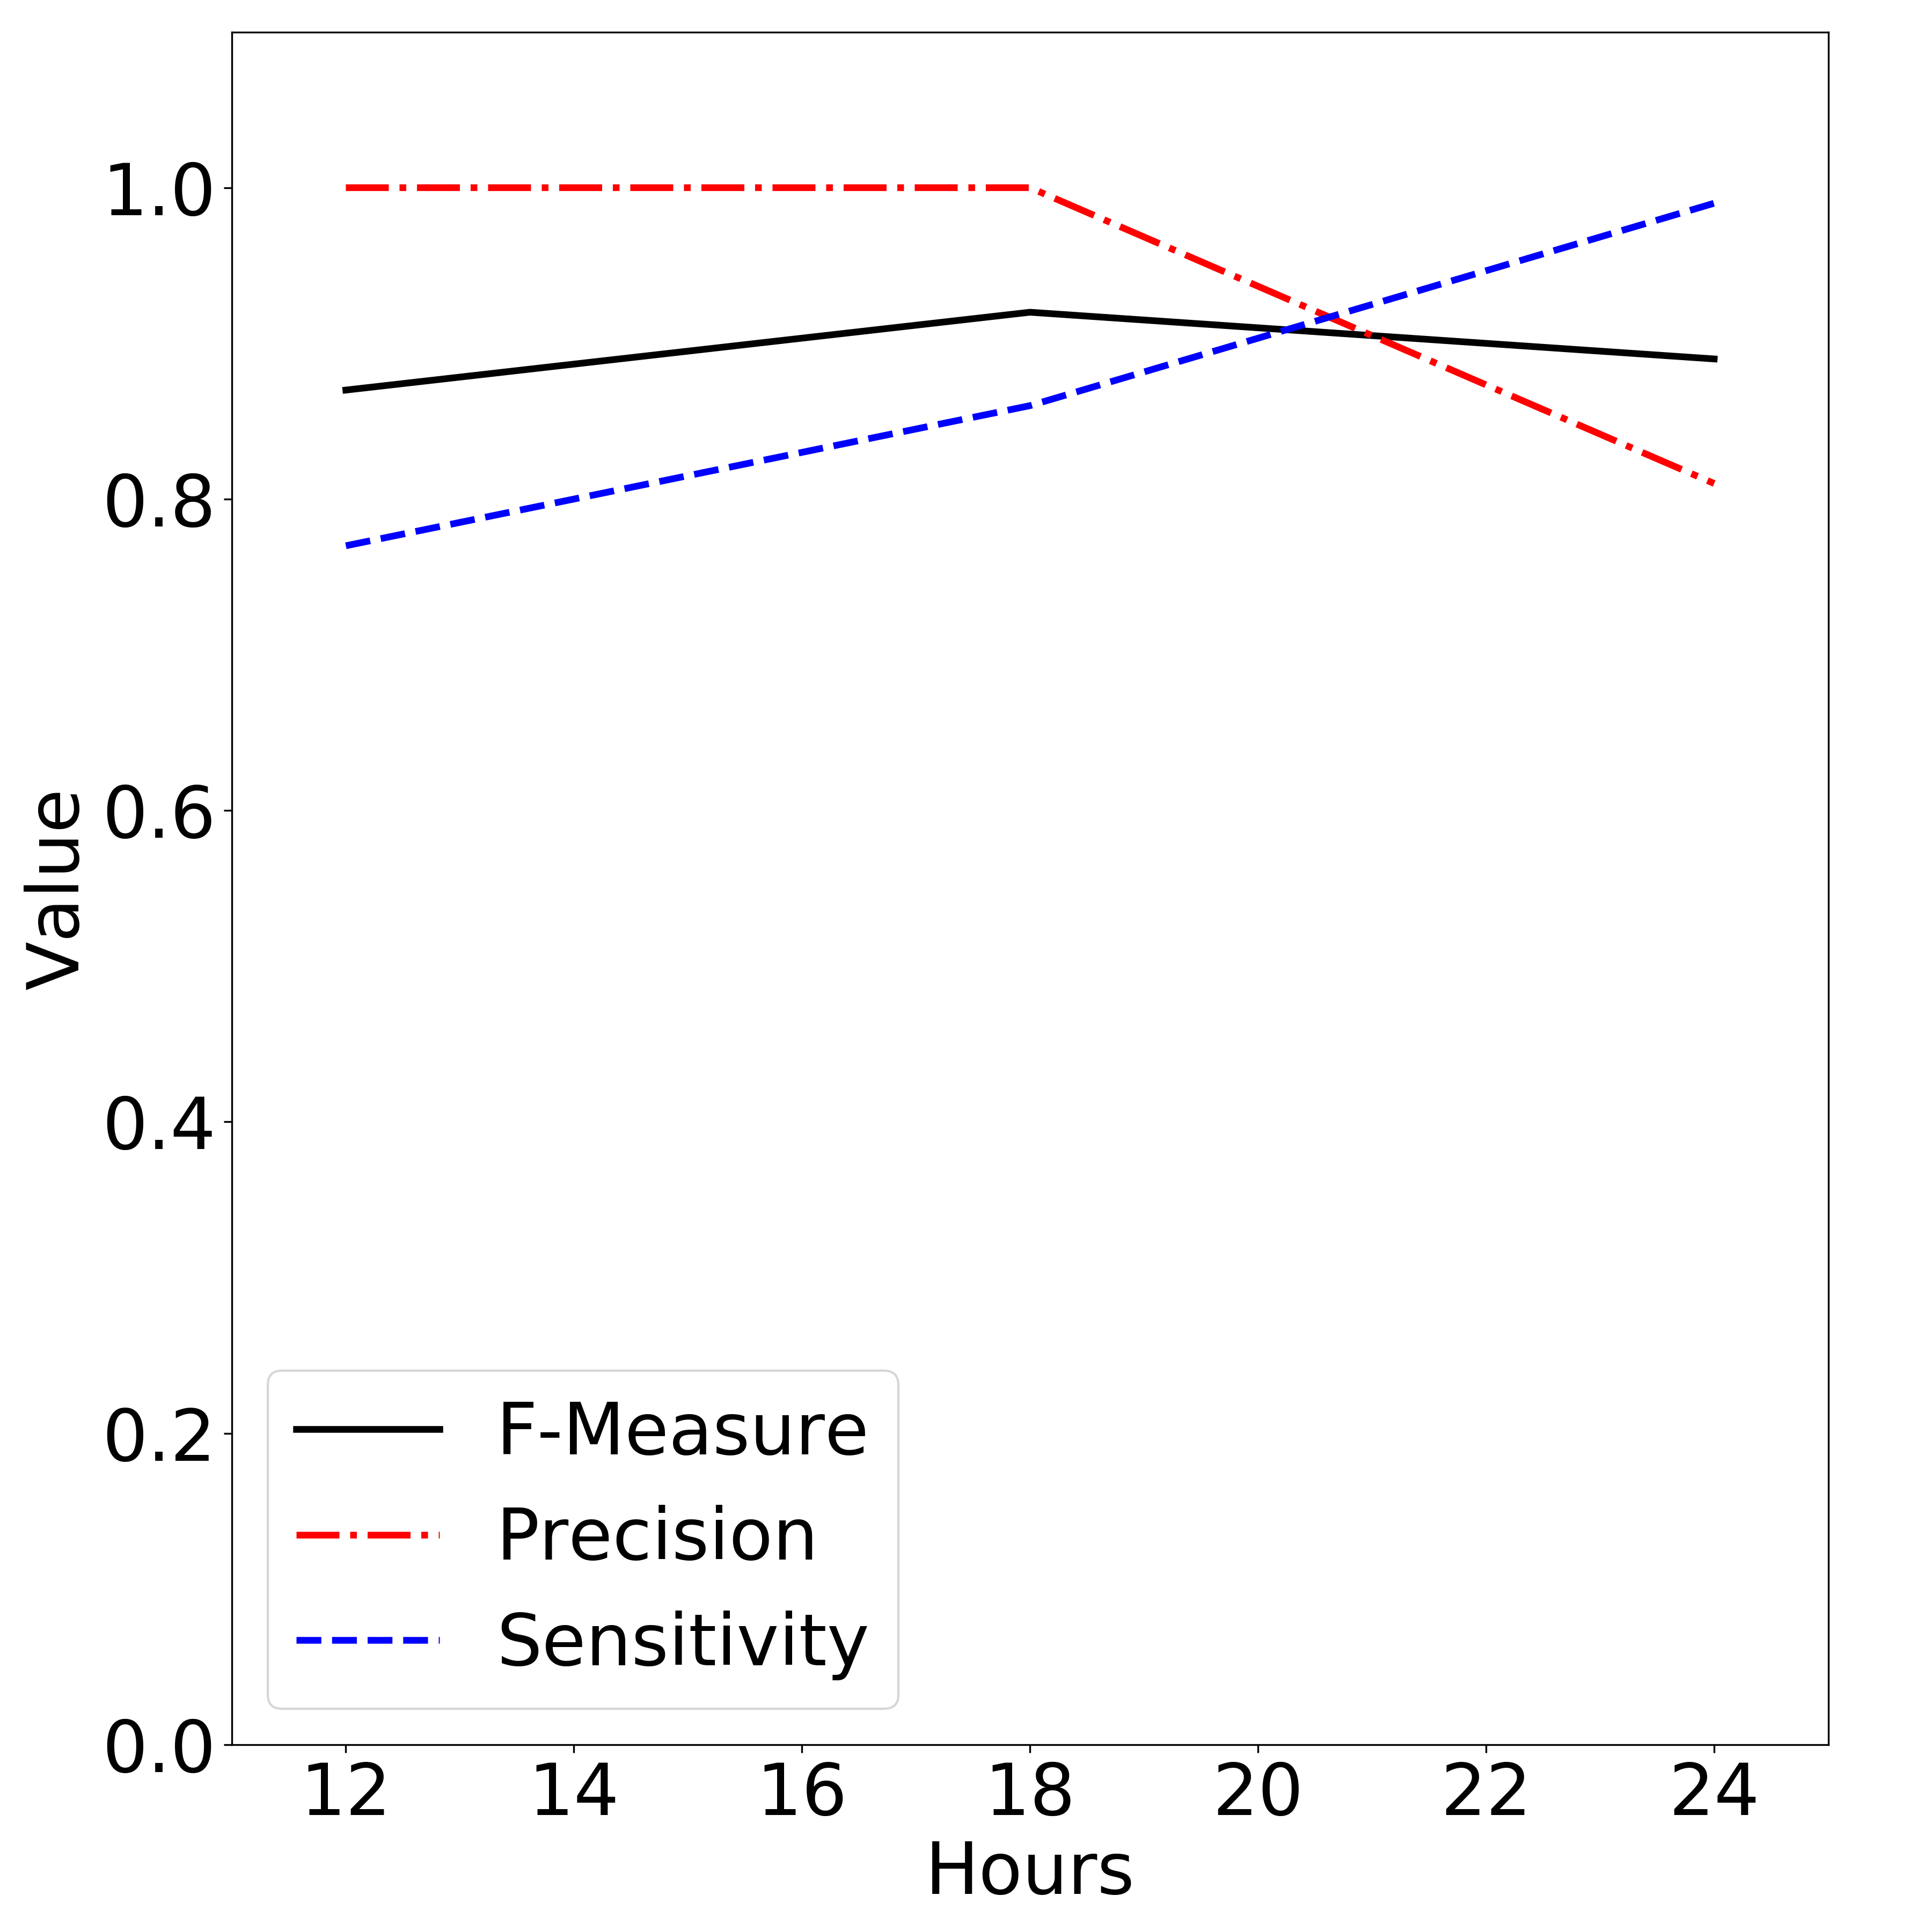
\includegraphics[height=0.25\textwidth]{timeAnalysis_fmeasure2.png}
	\\
	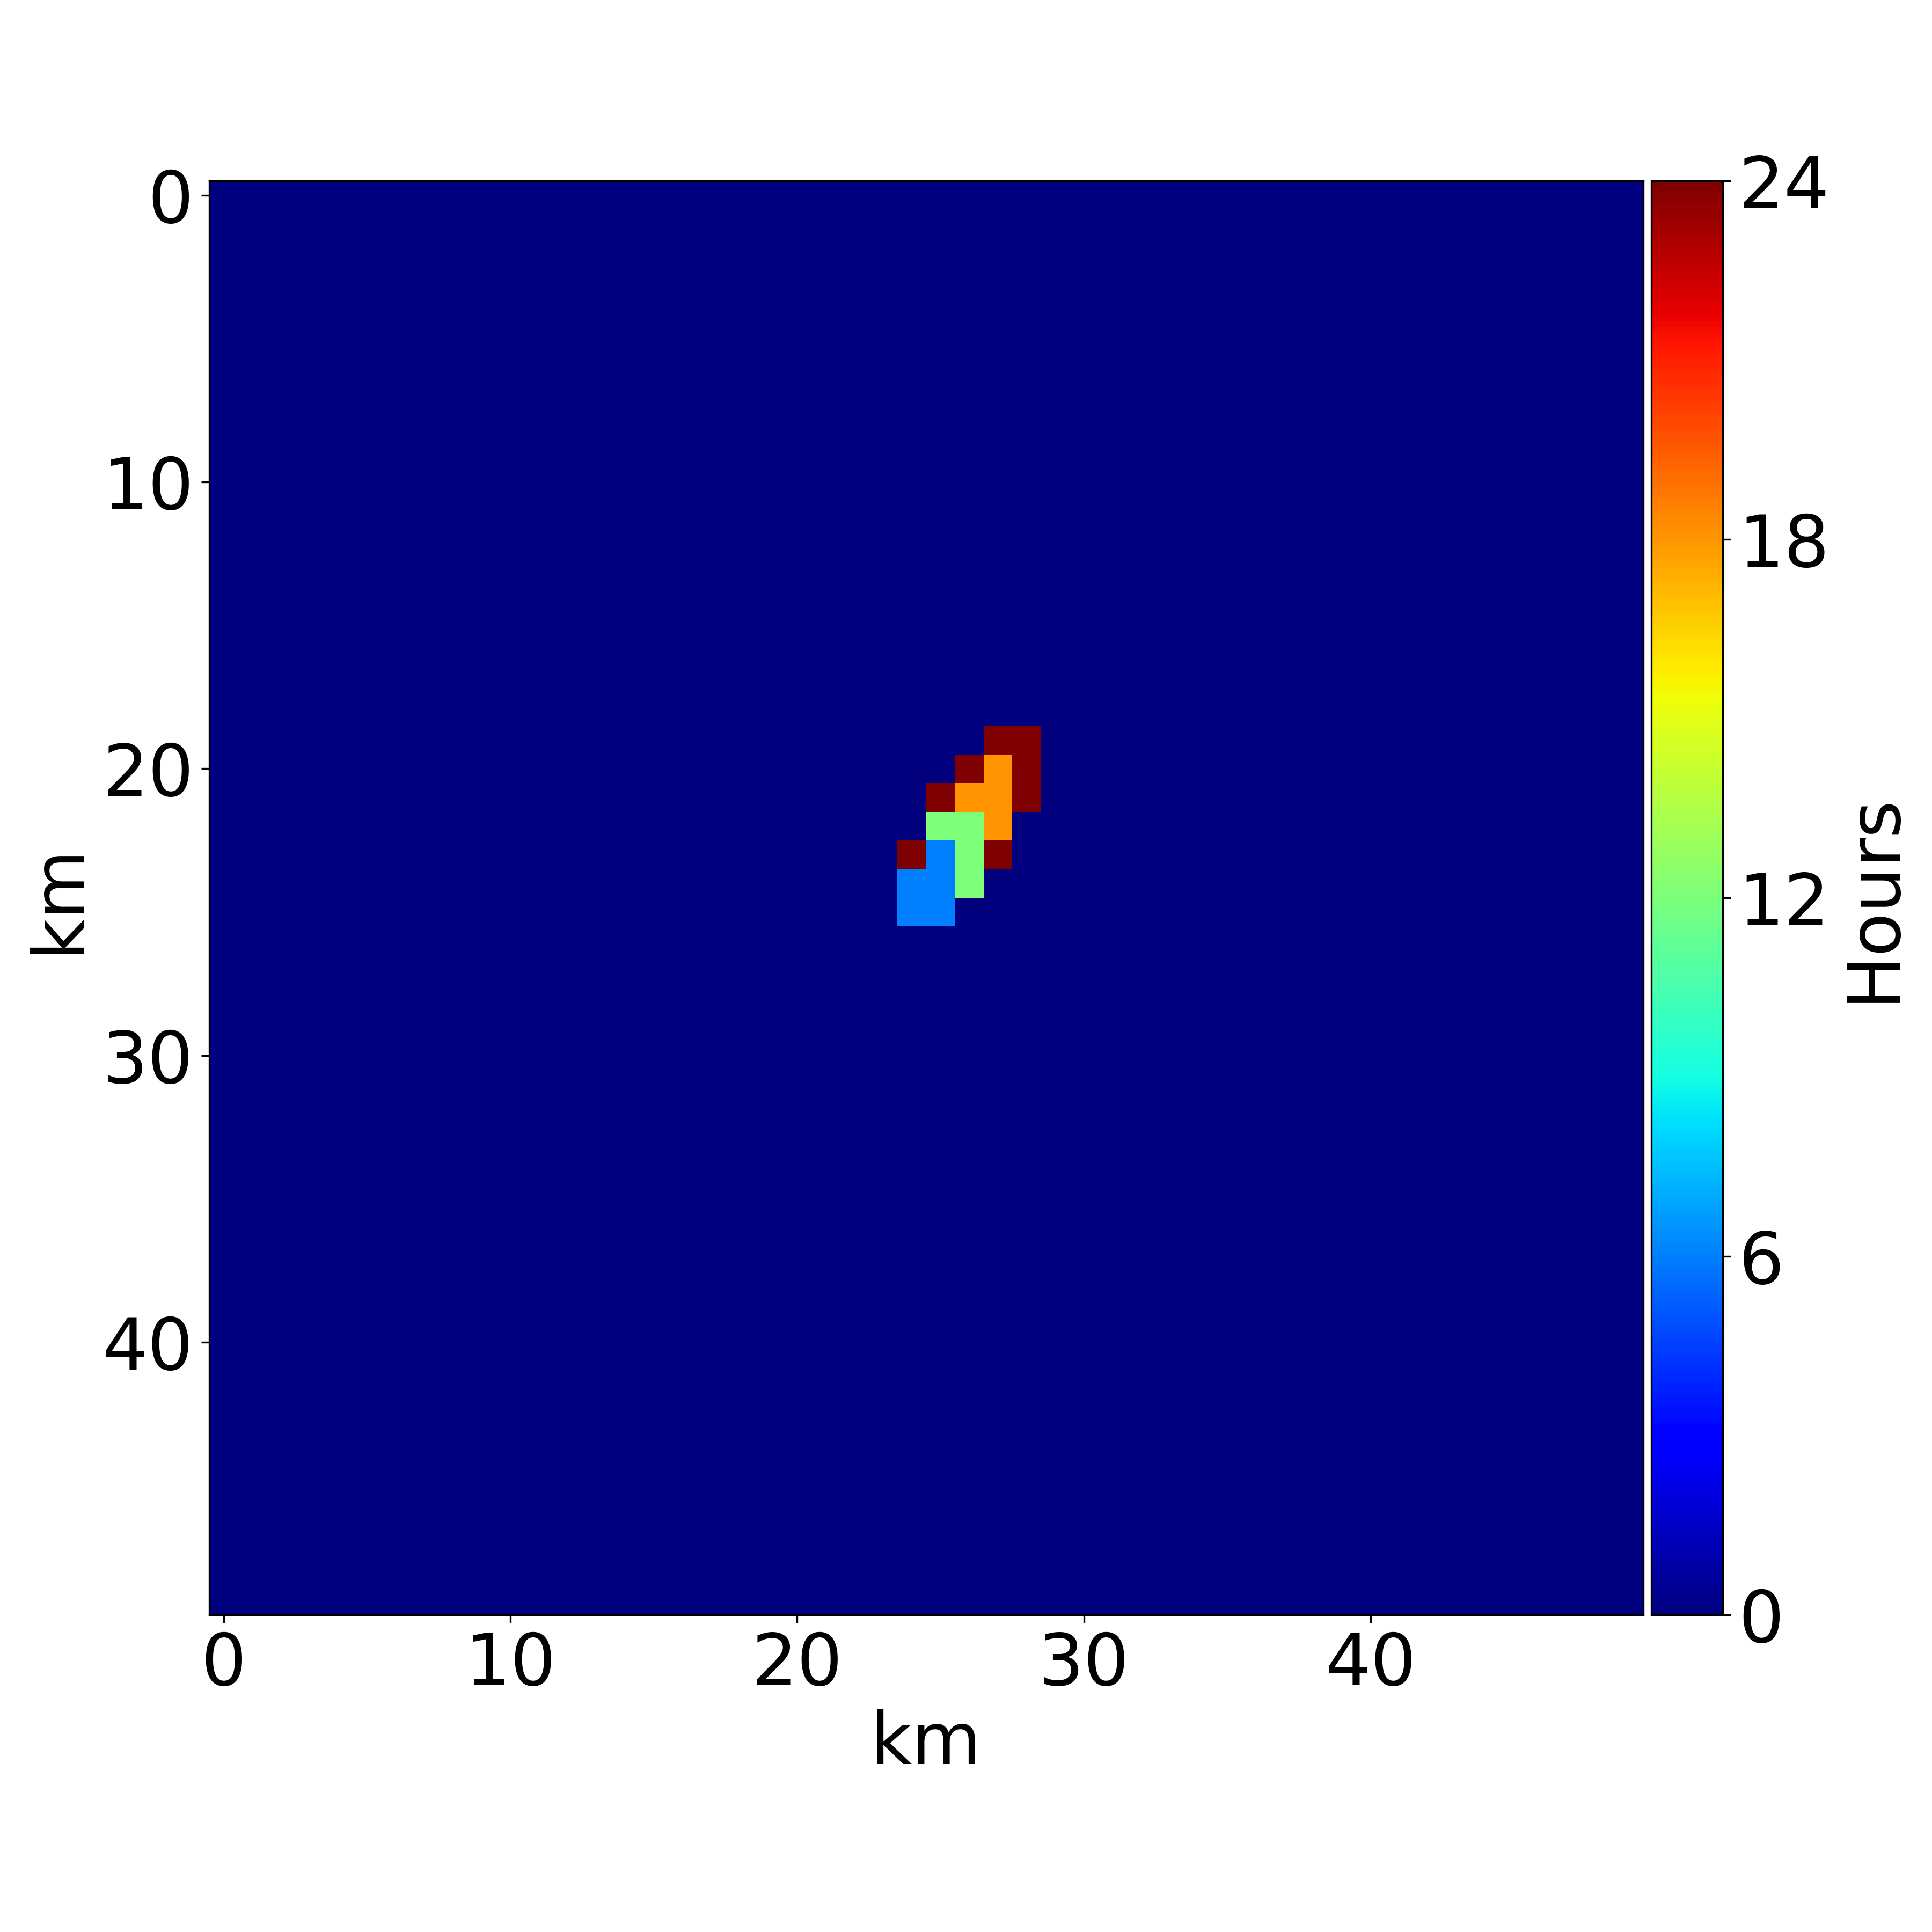
\includegraphics[height=0.25\textwidth]{timeAnalysis_simulation3.png}
	~
	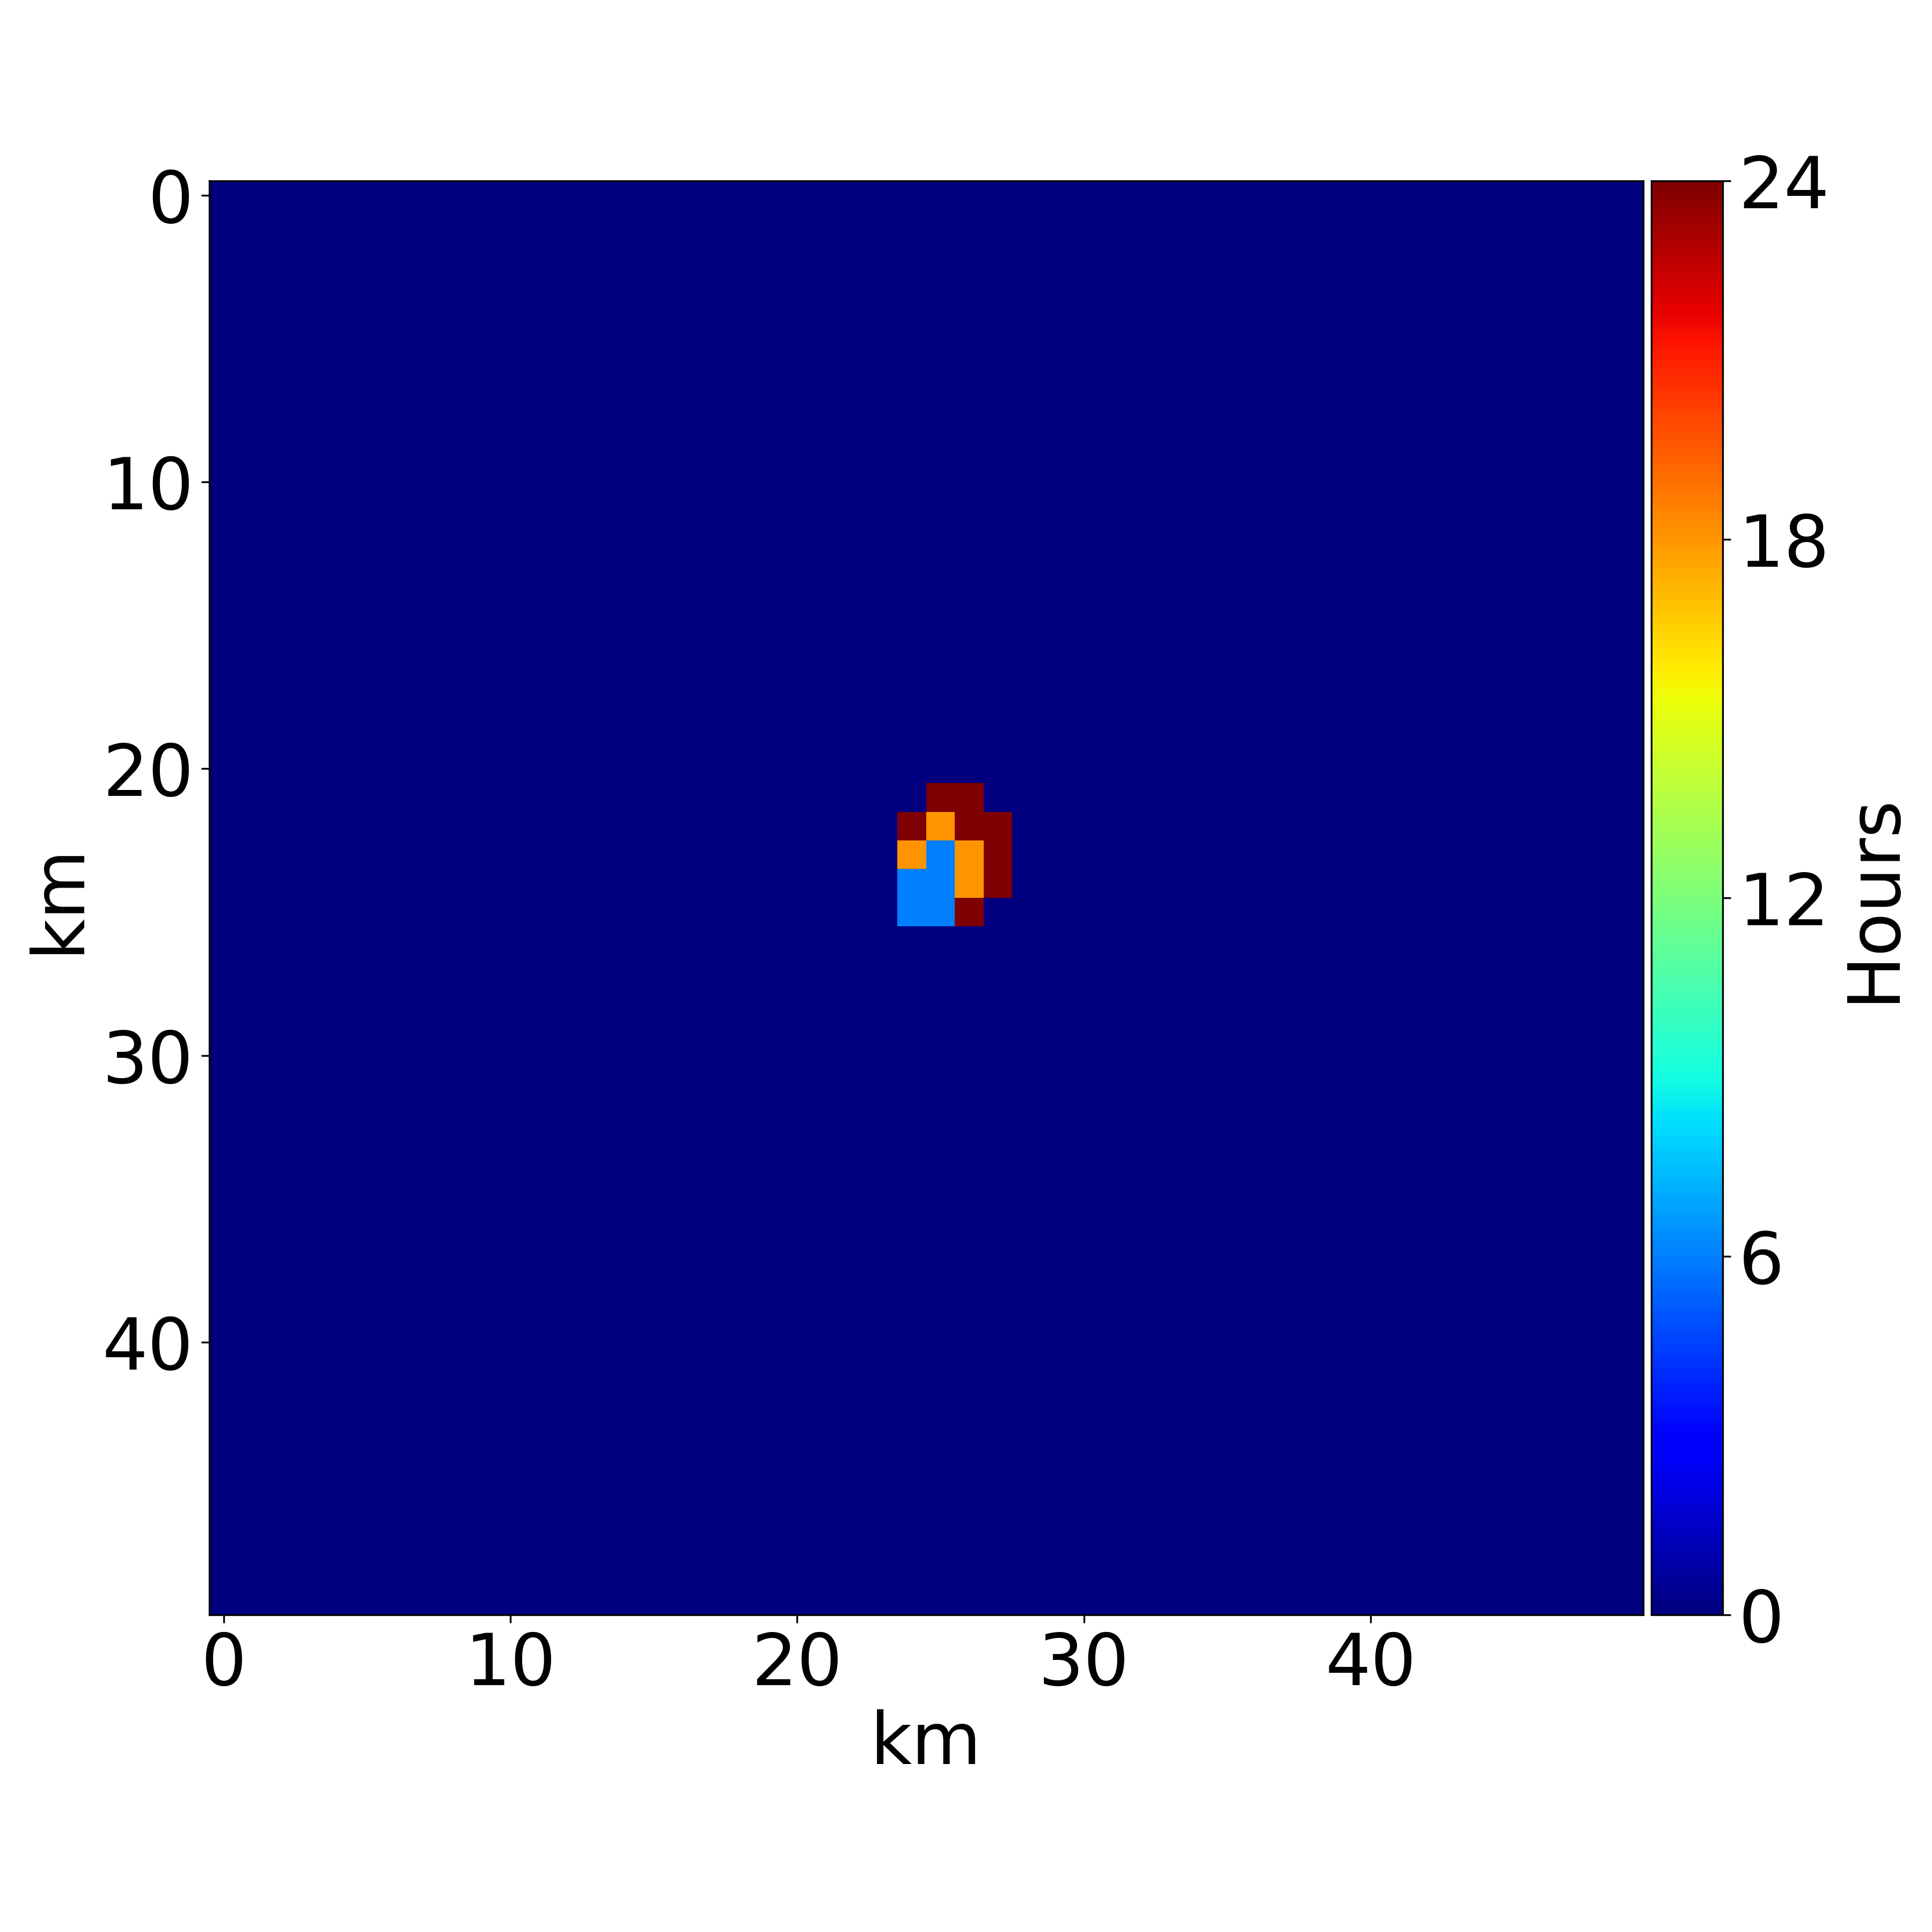
\includegraphics[height=0.25\textwidth]{timeAnalysis_network3.png}
	~
	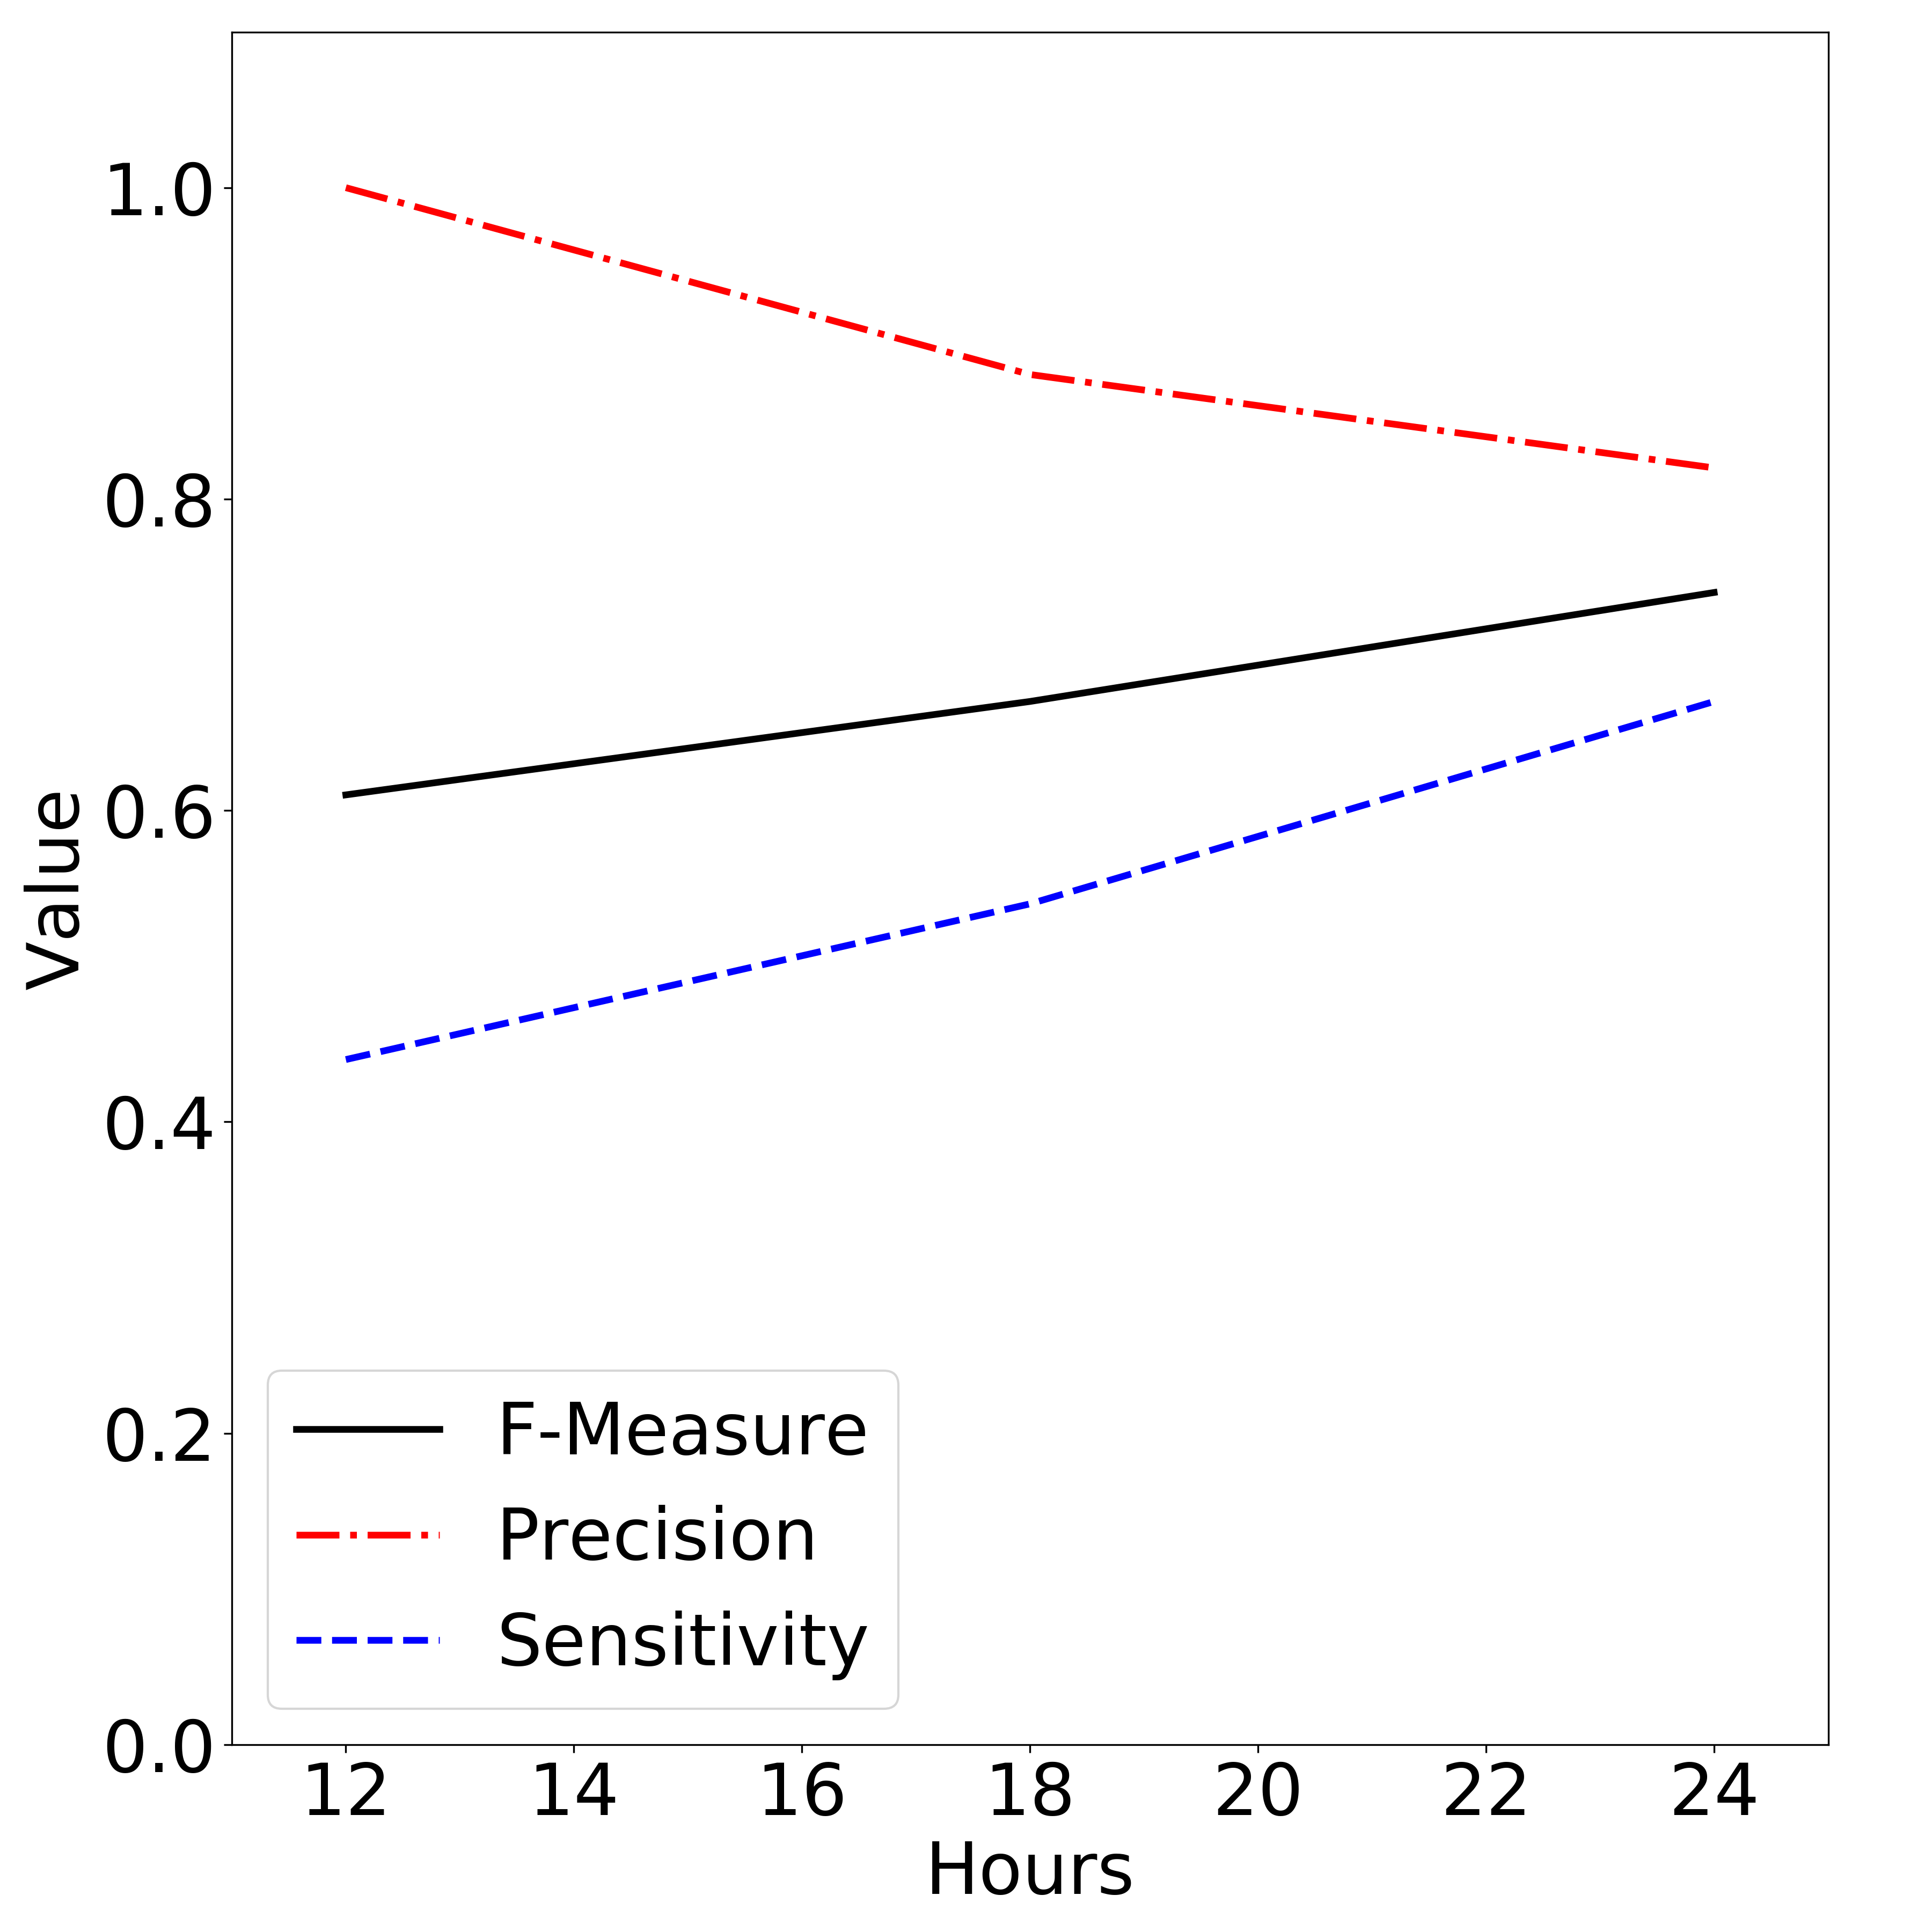
\includegraphics[height=0.25\textwidth]{timeAnalysis_fmeasure3.png}
	\\
	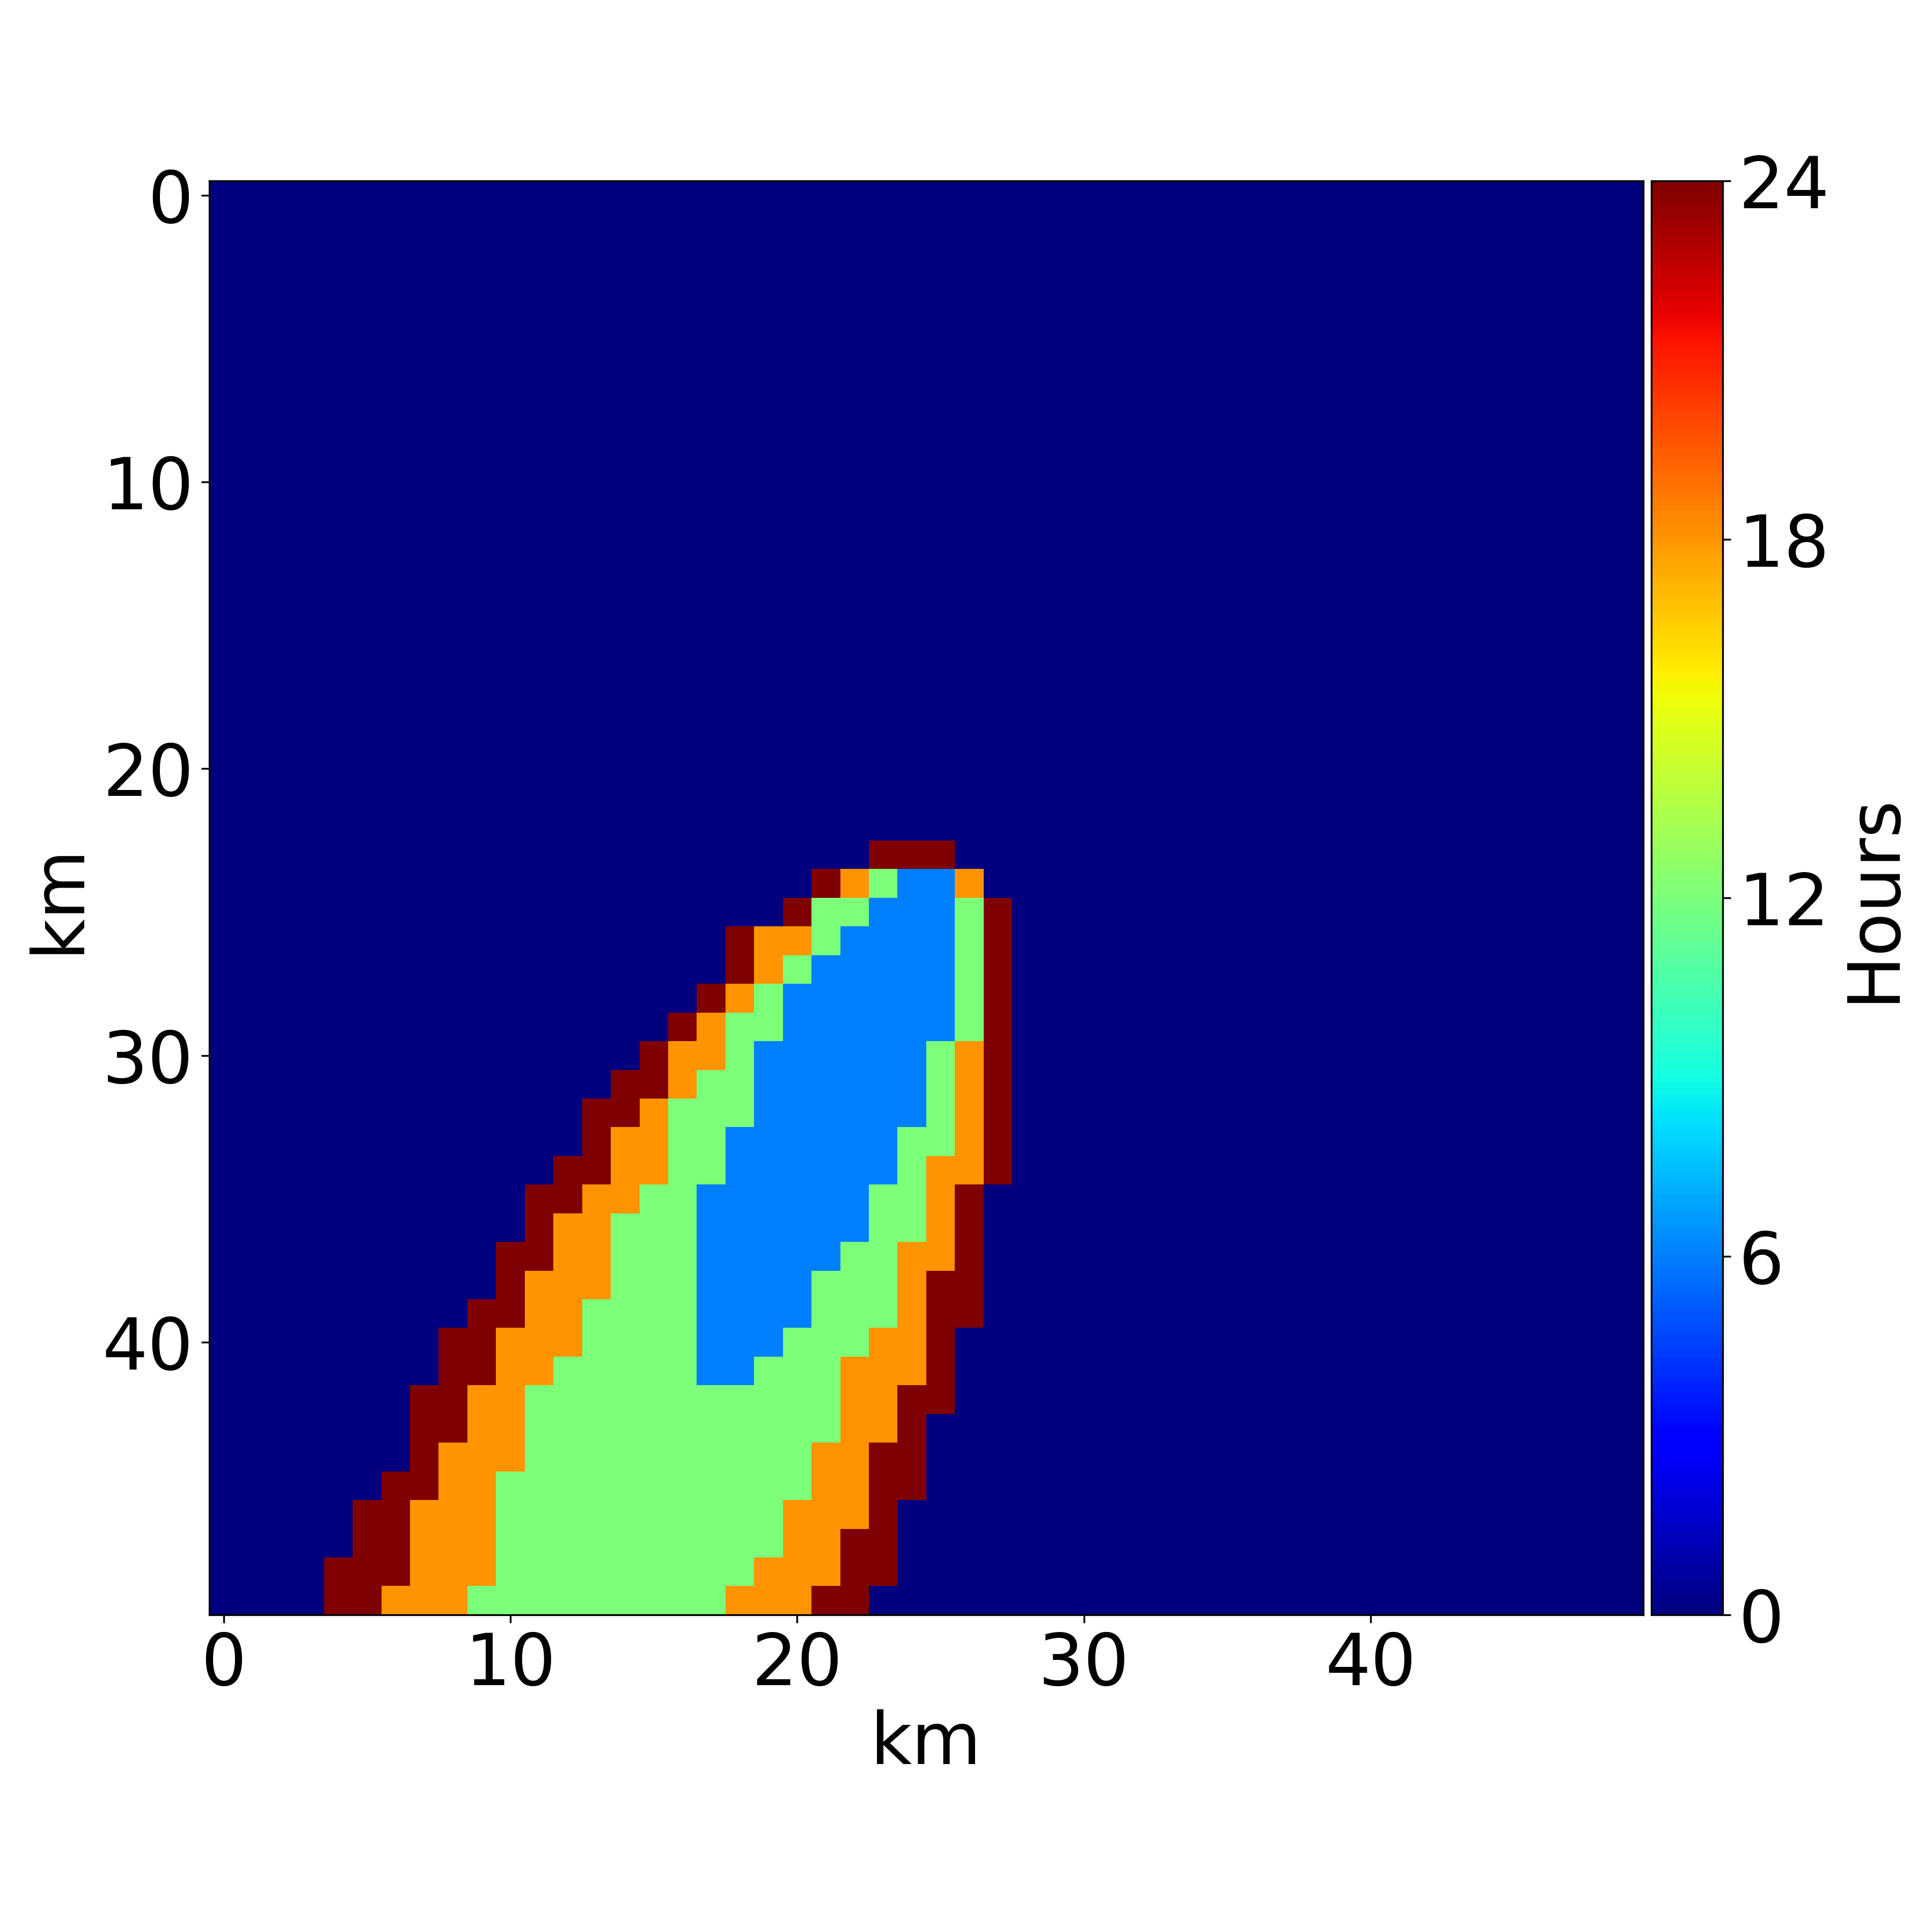
\includegraphics[height=0.25\textwidth]{timeAnalysis_simulation4.png}
	~
	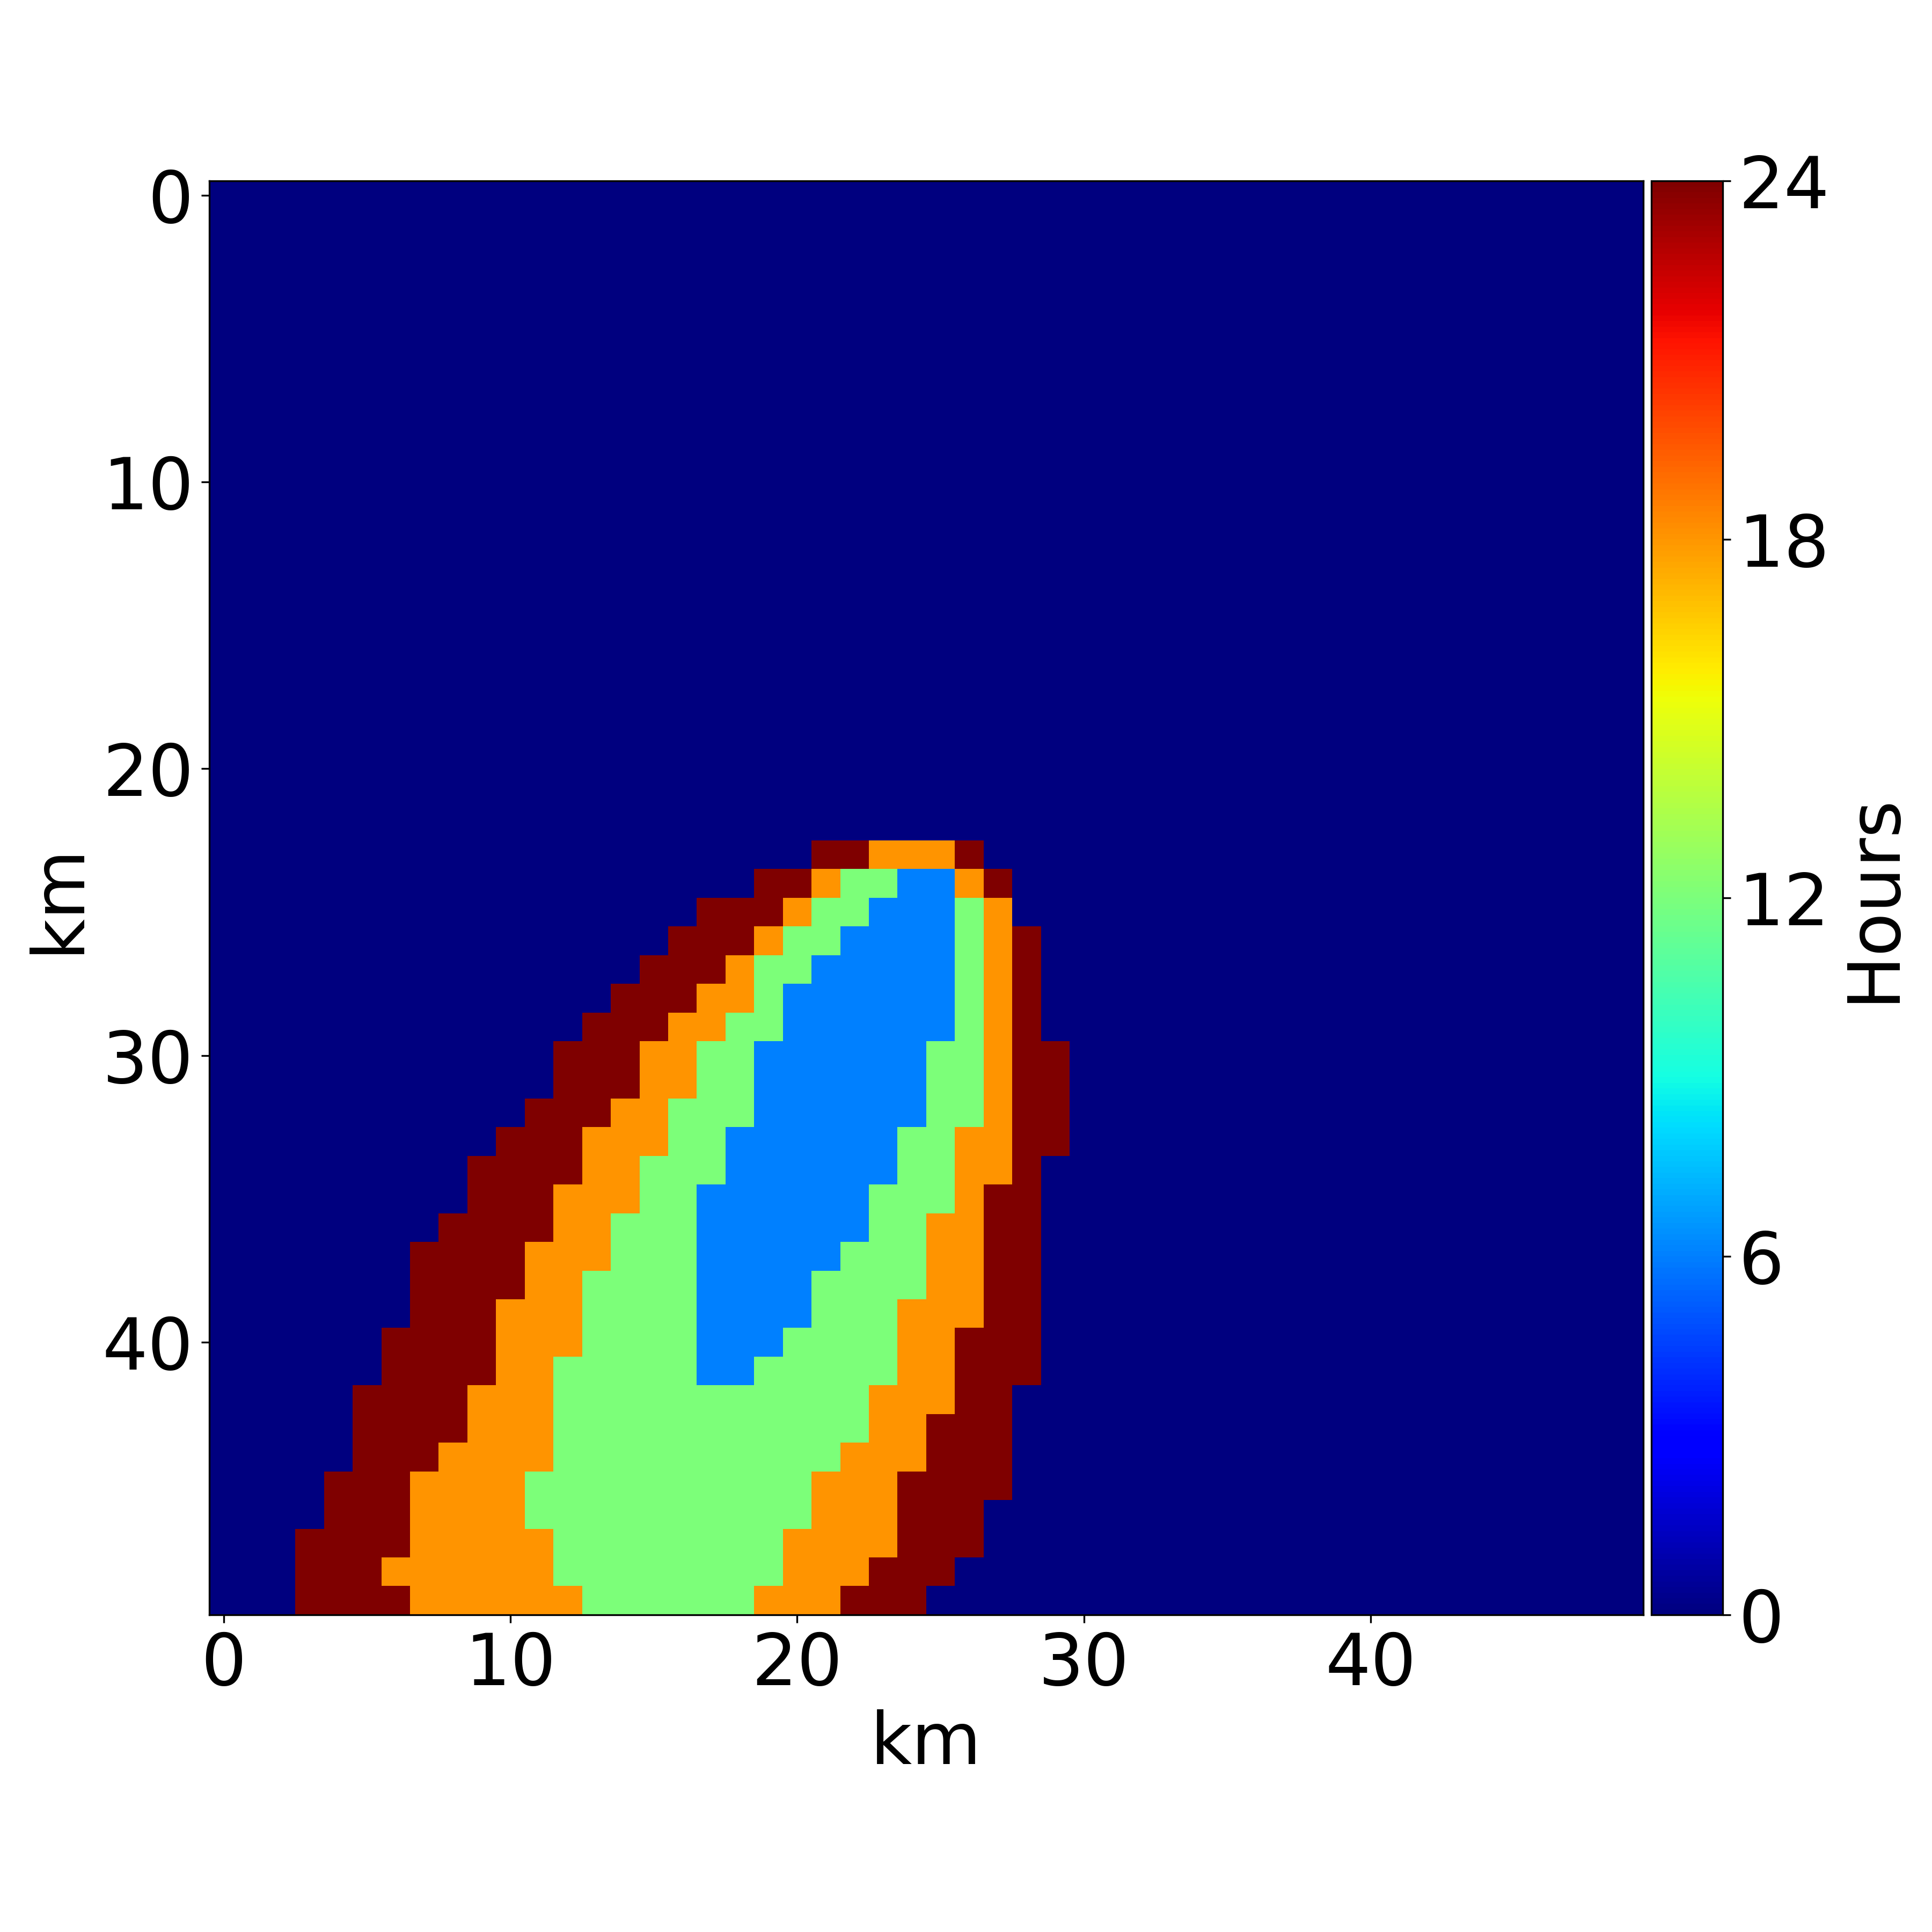
\includegraphics[height=0.25\textwidth]{timeAnalysis_network4.png}
	~
	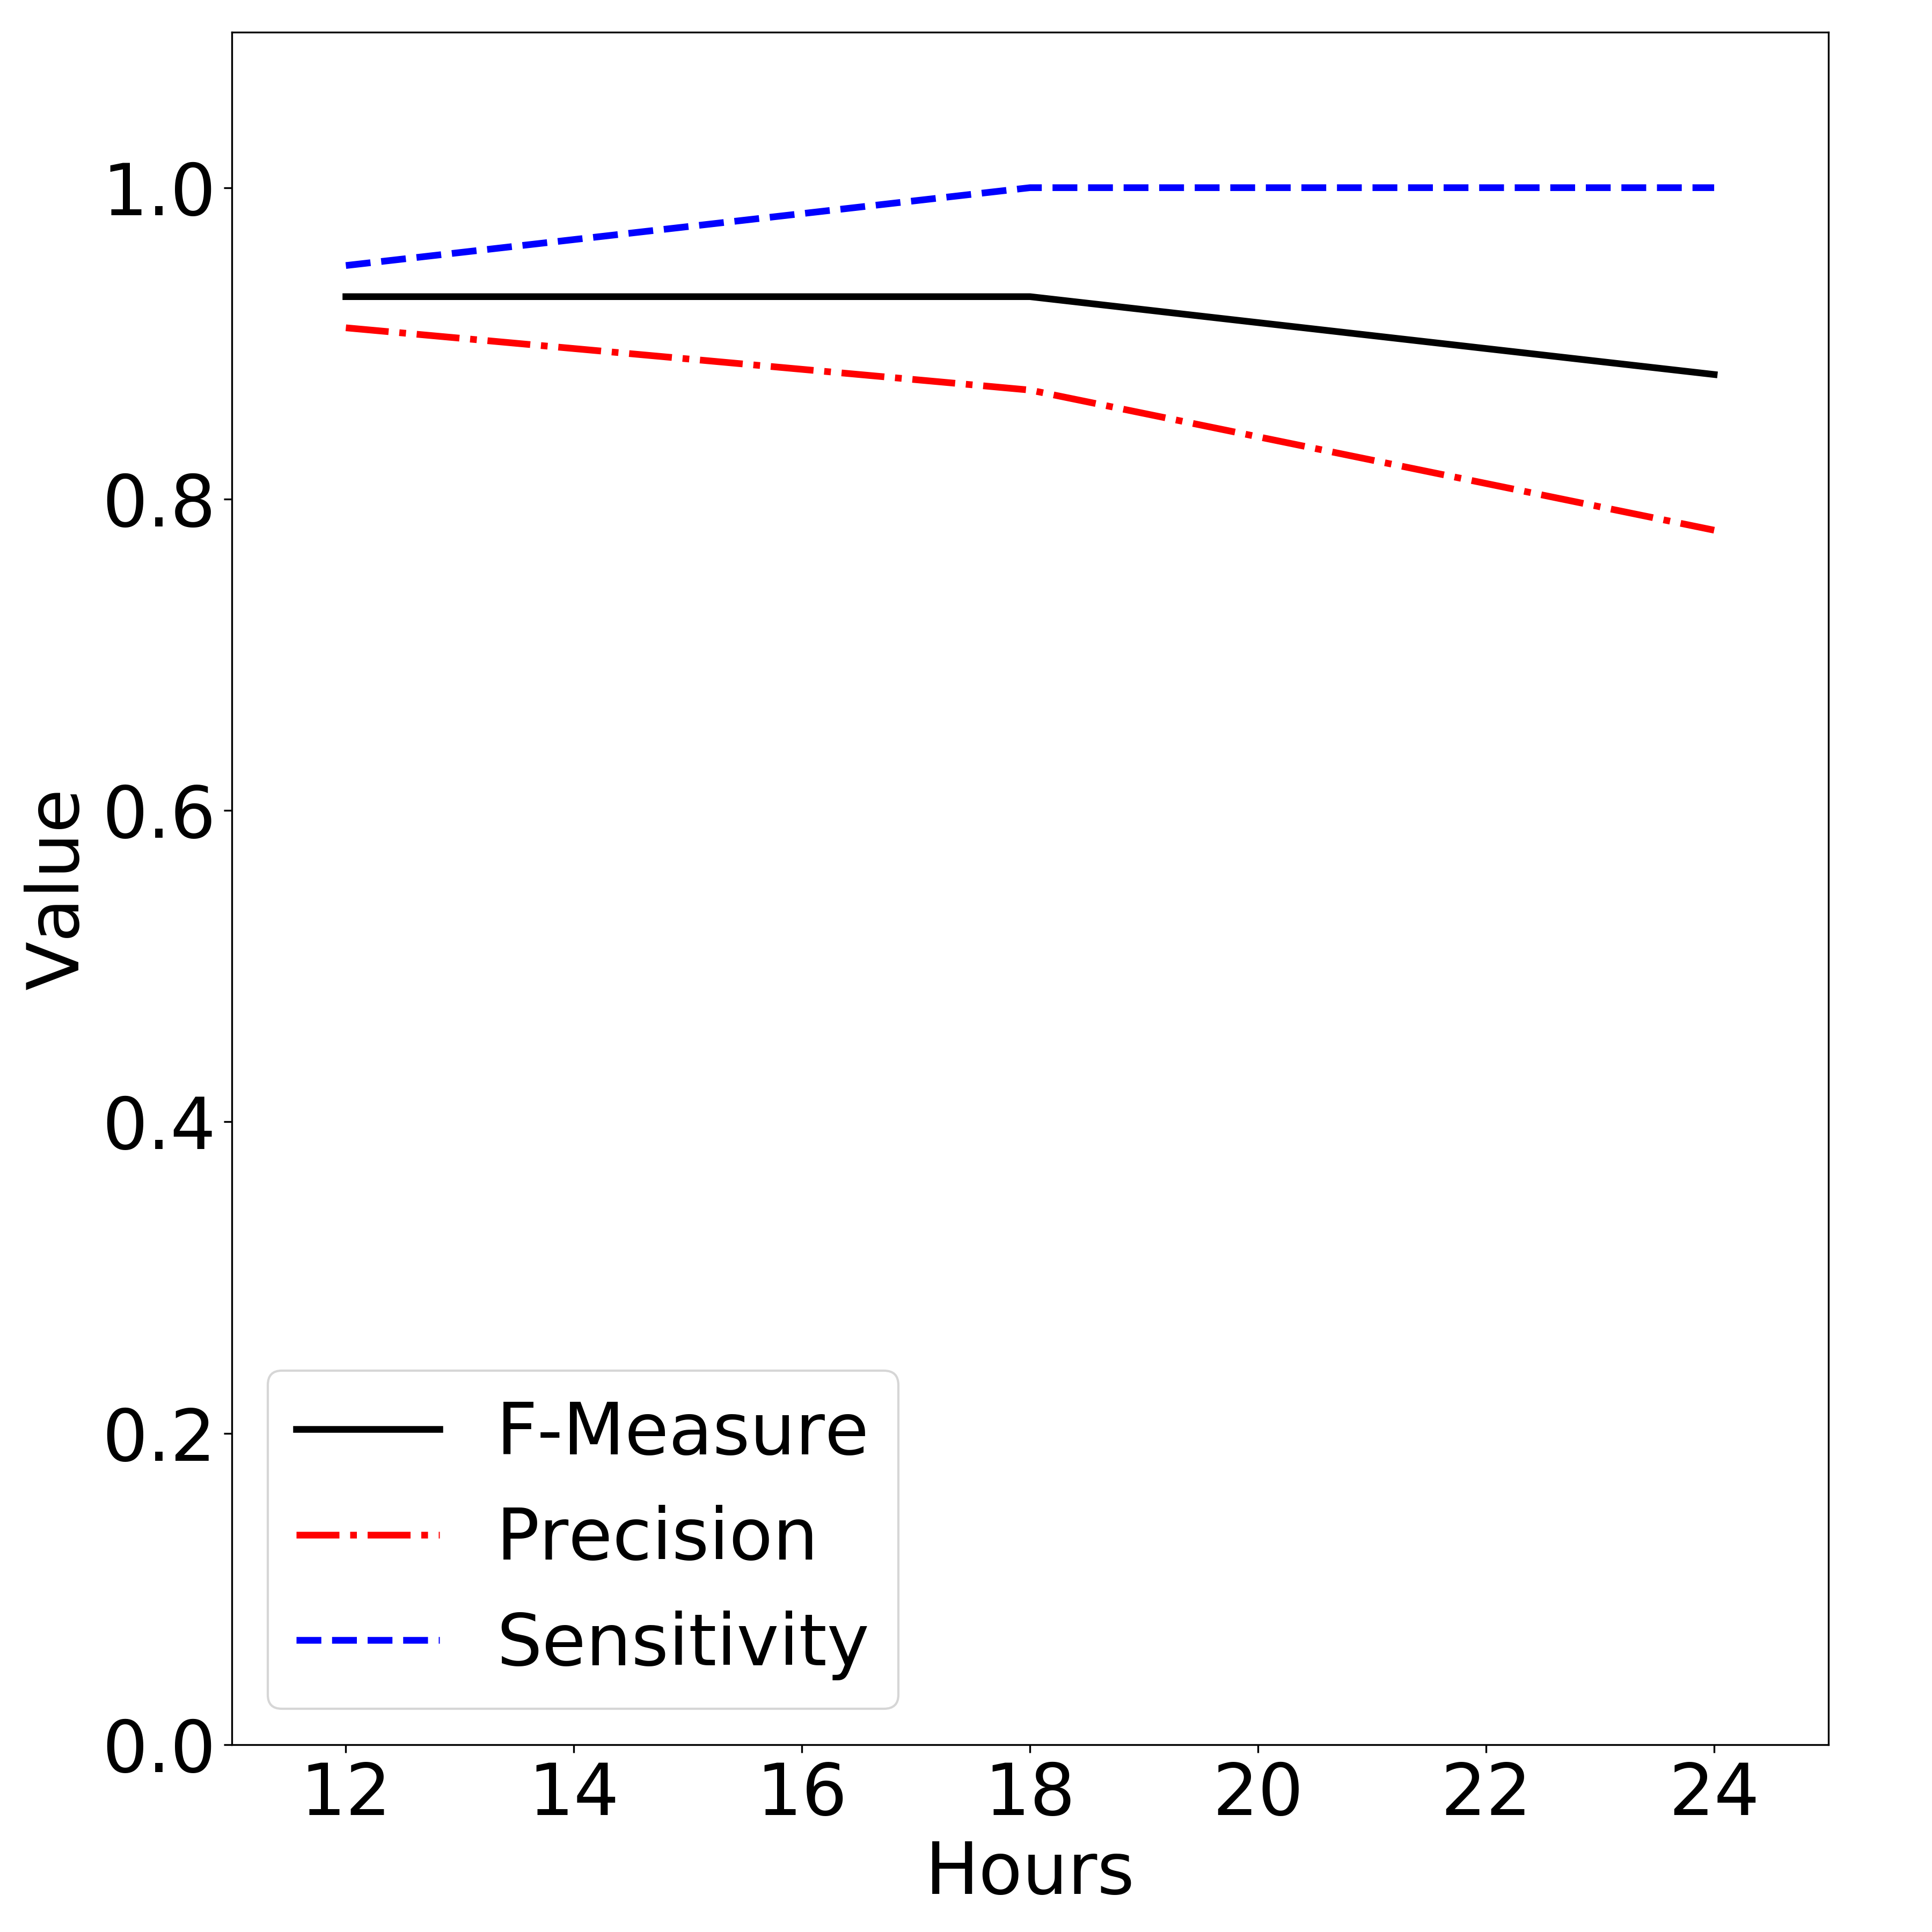
\includegraphics[height=0.25\textwidth]{timeAnalysis_fmeasure4.png}
	\\
\hspace{0.035\textwidth}(a)\hspace{0.29\textwidth}(b)\hspace{0.31\textwidth}(c)
\caption{Example CNN prediction of time resolved fire perimeters (a) Simulation fire perimiter (b) CNN prediction of fire perimeter (c) F-Measure at 6 hour intervals}
\label{fig:timeAnalysis}       % Give a unique label
\end{figure*}


The optimal threshold to use in post-processing was determined by calculating
the mean F-measure for CNN predictions of the 27,000 training cases with
thresholds ranging from 0.01 to 0.99.
The mean F-measure was found to be mostly independent of the post-processing threshold
in the range of 0.2-0.6 as shown in Fig.~\ref{fig:fMeasureVsThreshold}.
The maximum mean F-measure of the training data was calculated with a threshold
of 0.41. This threshold was fixed and used when analyzing the test cases.





The model was trained using a 6 hour time interval between the input
and output fire perimeters. It is possible to obtain predictions at points
further in the future at 6 hour intervals by recursively using the previous
prediction as an input to the CNN. Figure~\ref{fig:timeAnalysis} shows
5 example cases where this process was used to predict fire perimeters
up to 24 hours from ignition based on an input fire perimeter 6 hours after
ignition. The results for each case show the general direction of spread
is captured well, with $F > 0.8$ in all cases except the fourth case where
the input and output fires are small.
The sensitivity of the predictions generally increases
with time, whereas the precision generally decreases with time. Since
precision describes commission errors and sensitivity describes omission
errors, this shows early in the progression of the fire the model
under-predicts the rate of spread, but later on the model over-predicts
the rate of spread. This highlights the difficulty the CNN can have
when dealing with low feature density.






















\section{Conclusion}
\label{s:Conclusion}

A novel predictive analytics approach to predicting the spread of
a wildland fire using a convolutional neural network (CNN) was presented.
The robustness of the approach was tested using 3,000 test cases
which were not included when training the network. The predictions of
fire perimeter from the CNN based approach agreed with simulation results,
with a mean F-measure of 0.93. Cases where F-measure was observed to
be less than 0.80, 82\% contained less than 9 pixels in the input
fire perimeter. Although trained on predictions 6 hours apart, the
CNN-based approach is capable of predicting fire perimeters further
in the future by recursively using previous predictions as inputs to
the model. The model was found to be primarily limited by low feature
density in the input fire perimeter, typically from small fire
perimeters resulting from low rates of spread in the simulations.

This work represents a first step in creating a framework to predict
wildland fire spread without physics based models. Although the data
used to train the CNN in this work was generated using a phenomological
model, the model does not contain any concept over whether the data
is from a computational fluid dyanmics model, phenomological model, or
even experimental measurements of fire perimeter. Additionally, although
the simulations used were generated using homogenous vegetation and
landscapes, the feature learning aspect of the CNN based method is
well posed to learn heterogenous spatial conditions. The next step
in this process is to incorporate data from simulations with spatially
varying environmental conditions in the training and test sets.


% For one-column wide figures use
%\begin{figure}
% Use the relevant command to insert your figure file.
% For example, with the graphicx package use
%  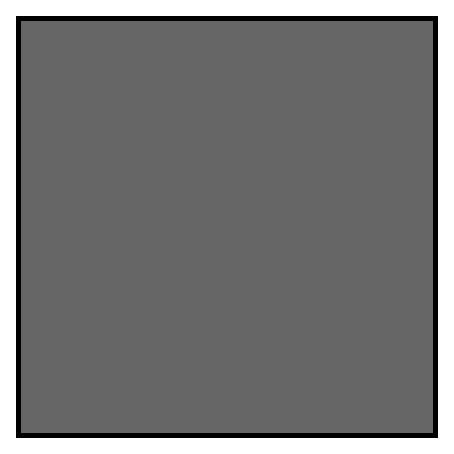
\includegraphics[width=0.5\textwidth]{example.eps}
% figure caption is below the figure
%\caption{Convolutional Neural Network Architecture}
%\label{fig:1}       % Give a unique label
%\end{figure}

%
%



%\begin{acknowledgements}
%If you'd like to thank anyone, place your comments here
%and remove the percent signs.
%\end{acknowledgements}

% BibTeX users please use one of
%\bibliographystyle{spbasic}      % basic style, author-year citations
%\bibliographystyle{spmpsci}      % mathematics and physical sciences
\bibliographystyle{spphys}       % APS-like style for physics
\bibliography{wildfireReferences}   % name your BibTeX data base

% Non-BibTeX users please use
%\begin{thebibliography}{}
%
% and use \bibitem to create references. Consult the Instructions
% for authors for reference list style.
%
%\bibitem{weber1991}
%Rodney O. Weber, Modelling fire spread through fuel beds, Progress in Energy and Combustion Science, 17, 67-82 (1991)
%\bibitem{rothermel1972}
%Richard C. Rothermel, A mathematical model for predicting fire spread in wildland fuels, U.S. Department of Agriculture, Forest Service, Ogden, UT (1972)
%\bibitem{scott2005}
%Joe H. Scott; Robert E. Burgan, Standard fire behavior fuel models: a comprehensive set for use with Rothermel's surface fire spread model, U.S. Department of Agriculture, Forest Service, Rocky Mountain Research Station, Fort Collins, CO (2005)

% Format for books
%\bibitem{RefB}
%Author, Book title, page numbers. Publisher, place (year)
%\end{thebibliography}

\end{document}

